\chapter{Random Coefficients Logit: The BLP Model}\label{ch:blp}

Suppose two car makers propose to merge. To predict the effect on prices we need to know how buyers of each
model would respond to a price increase, and where they would go. With a hundred models on the market, a demand
system in product space has ten thousand own- and cross-price elasticities (\cref{ch:aids}). The logit model of
\cref{ch:logit} needs only a handful of parameters, but it pays for its economy with substitution patterns that
depend on market shares alone. It predicts that buyers who leave a luxury sedan spread over all other models in
proportion to their sales, and that most of them stop buying cars altogether. Neither prediction is plausible,
and a merger analysis built on them would be wrong.

This chapter studies the model that resolves the tension, the \emph{random coefficients logit} of
\citet{BerryLevinsohnPakes1995}, often called BLP. Consumers differ in how much they value each characteristic
and how much they dislike paying. Each consumer makes a logit choice, and market shares average these choices
over the distribution of tastes. Consumers who like large cars rank all large cars highly, so a price increase
on one large car sends its buyers mostly to other large cars. Substitution follows the characteristics of the
products. The number of parameters grows with the number of characteristics, however many products the market
offers.

BLP solve three problems at once. The first is to obtain plausible substitution patterns among many products
from few parameters. The second is the endogeneity of prices when only market-level data on shares, prices and
characteristics are available. Firms see product quality that the econometrician does not, and they price
accordingly. The third is computation. The market shares of the model are integrals with no closed form, and the
unobserved quality enters them nonlinearly. BLP compute the integrals by simulation and recover unobserved
quality by inverting the share equations numerically. A generalized method of moments estimator then treats the
recovered quality as the error term of an instrumental variables problem.

The chapter builds directly on \cref{ch:logit}. There we derived the logit shares
$s_j = \frac{e^{\delta_j}}{1 + \sum_k e^{\delta_k}}$ and the inversion $\delta_j = \ln s_j - \ln s_0$ of
\citet{Berry1994}, which turns demand estimation into a linear instrumental variables regression. We also saw the
costs of the logit. Its own-price elasticity $\alpha p_j(1 - s_j)$ rises almost in proportion to price, and its
single-product markup $\frac{1}{\alpha(1 - s_j)}$ is nearly the same for every product. Its cross elasticities
satisfy the independence of irrelevant alternatives (IIA). The nested logit relaxes this property only within groups
of products that the researcher must specify in advance. Random coefficients instead generate correlation in the
composite error through the characteristics of the products, and the data determine how strong it is.

Mixtures of logits, known as \emph{mixed logit} or \emph{heterogeneous logit} models, were used in
transportation research well before BLP \citep{BoydMellman1980,CardellDunbar1980}. The innovation of
\citet{BerryLevinsohnPakes1995} is a computable estimator for aggregate data with endogenous prices, joined to a
model of oligopoly pricing. Their framework is now the standard tool for demand estimation in industrial
organization, with applications to mergers, trade policy, new goods and many other questions.

The chapter has a theoretical half and an empirical half. \Cref{sec:08-model,sec:08-substitution,sec:08-simulation}
specify the model, derive its substitution patterns and explain how to compute market shares by simulation.
\Cref{sec:08-inversion,sec:08-gmm,sec:08-instruments} develop the estimator. They prove that the share equations
can be inverted by a contraction, and they derive the nested fixed point GMM estimator and its asymptotic variance.
They then ask what instruments identify the model, including the nonparametric results of \citet{BerryHaile2014}.
\Cref{sec:08-supply,sec:08-micro,sec:08-practice} add the supply side, micro data and the practical and
conceptual limits of the model. \Cref{sec:08-worked} estimates the model step by step on a simulated market whose
true parameters we know. The empirical half consists of five case studies. \Cref{sec:08-blp95} studies the
automobile market of \citet{BerryLevinsohnPakes1995}, and \cref{sec:08-nevo00} the practitioner's guide of
\citet{Nevo2000a}. \Cref{sec:08-nevo01} turns to the cereal study of \citet{Nevo2001}. \Cref{sec:08-blp04,%
sec:08-goldberg} cover two studies that use consumer-level data, \citet{BerryLevinsohnPakes2004} and
\citet{Goldberg1995}.

We draw on several earlier chapters. Multiproduct Bertrand pricing, the ownership matrix and the distinction
between product space and characteristic space come from \cref{ch:diffprod}. Random utility, the outside good,
the vertical model and the pure characteristics model come from \cref{ch:discrete}. The generalized method of
moments, instrumental variables and simulation estimators are reviewed in
\cref{sec:A-gmm,sec:A-iv,sec:A-simulation}, and the contraction mapping and implicit function theorems in
\cref{sec:B-fixedpoint,sec:B-ift}. In turn, \cref{ch:airlines} uses a two-type
version of the model, \cref{ch:newgoods} uses it to value new products, and \cref{ch:mergers} uses it to simulate
mergers. \Cref{app:problems} poses the simulated market of \cref{sec:08-worked} as a worked problem.

Two conventions hold throughout the chapter. The symbol $\theta$ denotes a vector of demand and cost parameters,
split into linear parameters $\theta_1$ and nonlinear parameters $\theta_2$. It is unrelated to the conduct
parameter of \cref{ch:conduct}. The elasticity $\varepsilon_{jk} = \frac{\partial s_j}{\partial p_k}\frac{p_k}{s_j}$
is signed, so its diagonal element $\varepsilon_{jj}$ is negative. In the theory sections the own-price elasticity
$\varepsilon_j = -\varepsilon_{jj}$ is a positive number. Tables reproduced from papers keep the papers' signs, and
their notes say so.

\section{The random coefficients logit model}\label{sec:08-model}

The random coefficients logit model describes a population of consumers who differ in how much they value
each product characteristic and how much they dislike paying. Each consumer makes a logit choice given her
tastes. Market shares average these individual choice probabilities over the distribution of tastes in the
population. This section builds the model in steps. We start from the general random utility formulation of
\citet{BerryLevinsohnPakes1995} and specialize it to the linear form used in most applications
\citep{Nevo2000a,Nevo2001}. We then discuss income effects, normalizations and the maintained assumptions. The
section ends with the market share function, special cases, the role of the unobserved product characteristic,
and the data the model requires.

\subsection{Primitives}\label{sec:08-primitives}

We observe markets $t = 1, \dots, T$. A \emph{market} is a population of consumers who face the same set of
products at the same prices. Its definition depends on the data. \citet{BerryLevinsohnPakes1995} treat the
national new car market in each year from 1971 to 1990 as a market, so $T = 20$. \citet{Nevo2001} observes
ready-to-eat cereal sales in a panel of cities and defines a market as a city-quarter, which gives 1,124
markets \citep[p.~517]{Nevo2000a}. Other studies split one geographic market into income groups
\citep[p.~517]{Nevo2000a}.

Market $t$ offers the inside products $j \in \mathcal{J}_t = \{1, \dots, J_t\}$ and an outside good $j = 0$,
which stands for not buying any of the inside products. The market has $M_t$ potential consumers, its
\emph{market size}. If $q_{jt}$ units of product $j$ are sold, its market share is
$s_{jt} = \frac{q_{jt}}{M_t}$, and the outside share is $s_{0t} = 1 - \sum_{j \in \mathcal{J}_t} s_{jt}$.
Product $j$ has a row vector of $K$ observed characteristics $x_{jt}$, a price $p_{jt}$, and an
\emph{unobserved product characteristic} $\xi_{jt}$. Consumers and firms observe $\xi_{jt}$. The
econometrician does not.

Consumer $i$ is described by a vector of characteristics $\zeta_i$, which may include income, demographics,
and tastes that no data set records. In the general formulation of \citet[p.~845]{BerryLevinsohnPakes1995},
the utility of consumer $i$ from product $j$ is a scalar function
\begin{equation}\label{eq:08-general-utility}
  U(\zeta_i, p_{jt}, x_{jt}, \xi_{jt}; \theta),
\end{equation}
where $\theta$ is a vector of parameters. It includes the parameters of the utility surface and those of the
distribution of $\zeta_i$. Throughout this chapter $\theta$ denotes this vector of demand (and later cost)
parameters.

Consumer $i$ buys product $j$ if and only if $j$ gives her the highest utility. The set of consumer types who
choose $j$ is
\begin{equation}\label{eq:08-choice-set}
  A_{jt}(\theta) = \bigl\{\zeta : U(\zeta, p_{jt}, x_{jt}, \xi_{jt}; \theta) \ge
    U(\zeta, p_{rt}, x_{rt}, \xi_{rt}; \theta) \text{ for } r = 0, 1, \dots, J_t\bigr\}.
\end{equation}
Suppose ties occur with probability zero and let $P_0$ be the distribution of $\zeta$ in the population. The
market share of product $j$ is the mass of consumers in $A_{jt}$,
\begin{equation}\label{eq:08-share-general}
  s_{jt}(p_t, x_t, \xi_t; \theta) = \int_{\zeta \in A_{jt}(\theta)} P_0(\dd\zeta),
\end{equation}
which is equation (2.2) of \citet[p.~845]{BerryLevinsohnPakes1995}. Here $p_t$, $x_t$ and $\xi_t$ collect the
prices and characteristics of all products in market $t$. Demand for product $j$ is $q_{jt} = M_t
s_{jt}(p_t, x_t, \xi_t; \theta)$. Every product's demand depends on the prices and characteristics of all
products, because they shape the sets $A_{jt}$.

\citet[p.~521]{Nevo2000a} splits $\zeta_i$ into three parts: observed demographics $D_i$, unobserved
consumer characteristics $\nu_i$, and product-specific shocks $(\epsilon_{i0t}, \dots, \epsilon_{iJt})$. The
labels ``observed'' and ``unobserved'' refer to auxiliary data. We know something about the distribution of
$D_i$ (for example from a population survey), and nothing about the distribution of $\nu_i$ beyond a
parametric assumption. With this split, \eqref{eq:08-share-general} factors as
\begin{align}
  s_{jt} &= \int_{A_{jt}} \dd P^*(D, \nu, \epsilon) \notag\\
         &= \int_{A_{jt}} \dd P^*(\epsilon \mid D, \nu)\, \dd P^*(\nu \mid D)\, \dd P^*(D) \notag\\
         &= \int_{A_{jt}} \dd P^*_\epsilon(\epsilon)\, \dd P^*_\nu(\nu)\, \dd \hat P_D(D),
  \label{eq:08-share-bayes}
\end{align}
where $P^*$ denotes population distributions and $\hat P_D$ the distribution of demographics taken from
auxiliary data \citep[eq.~(4)]{Nevo2000a}. The second line is the factorization of a joint distribution into
conditional distributions. The third line uses the independence of $\epsilon$, $\nu$ and $D$, which we assume
below.

\subsection{The linear random coefficients specification}\label{sec:08-linear}

Most applications use a utility that is linear in characteristics and price. Let $u_{ijt}$ be the
\emph{conditional indirect utility} of consumer $i$ from product $j$ in market $t$, her indirect utility
conditional on choosing $j$. \citet[eq.~(1)]{Nevo2000a} specifies
\begin{equation}\label{eq:08-nevo-utility}
  u_{ijt} = \alpha_i (y_i - p_{jt}) + x_{jt}\beta_i + \xi_{jt} + \epsilon_{ijt},
\end{equation}
where $y_i$ is income and $\alpha_i$ is the marginal utility of income. The $K \times 1$ vector
$\beta_i$ holds her taste coefficients, and $\epsilon_{ijt}$ is a mean-zero idiosyncratic shock. The term
$\alpha_i(y_i - p_{jt})$ is the utility of the income left for other goods. It is linear in income, so the
specification comes from a quasilinear direct utility with no income effects.

The taste coefficients vary across consumers with observed and unobserved characteristics. We stack the
characteristics that may carry random coefficients into the row vector
$\tilde x_{jt} = (x_{jt}, p_{jt})$ of dimension $K + 1$, and the corresponding coefficients into the column
vector $b_i = (\beta_i^\T, -\alpha_i)^\T$. The model of taste heterogeneity is
\begin{equation}\label{eq:08-tastes}
  b_i = \begin{pmatrix} \beta_i \\ -\alpha_i \end{pmatrix}
      = \begin{pmatrix} \beta \\ -\alpha \end{pmatrix} + \Pi D_i + \Sigma \nu_i,
  \qquad \nu_i \sim F_\nu, \qquad D_i \sim F_{Dt}.
\end{equation}
Here $D_i$ is a $d \times 1$ vector of demographics with a market-specific distribution $F_{Dt}$. The
$(K+1) \times 1$ vector $\nu_i$ holds unobserved tastes with a known distribution $F_\nu$, usually the standard
normal $N(0, I_{K+1})$. The $(K+1) \times d$ matrix $\Pi$ measures how tastes vary with demographics, and the
$(K+1) \times (K+1)$ matrix $\Sigma$ scales the unobserved tastes \citep[eq.~(2)]{Nevo2000a}. With standard normal
$\nu_i$, the matrix $\Sigma\Sigma^\T$ is the covariance matrix of the unobserved part of tastes.
Applications usually take $\Sigma$ diagonal, so that $\sigma_k$ is the standard deviation of the
unobserved taste for characteristic $k$.\footnote{\citet[eq.~(2)]{Nevo2000a} and \citet[eq.~(3)]{Nevo2001}
order the coefficient vector as $(\alpha_i, \beta_i^\T)^\T$, with the price coefficient entering utility
as $-\alpha_i p_{jt}$. The two conventions differ only in the order of the rows and in the sign of the price
row of $\Pi$ and $\Sigma$.}

The last element of \eqref{eq:08-tastes} gives the price coefficient. Let $\iota_p$ be the $(K+1) \times 1$ vector
that selects the price element. Then
\begin{equation}\label{eq:08-alpha-i}
  \alpha_i = \alpha - \iota_p^\T(\Pi D_i + \Sigma \nu_i).
\end{equation}
Price therefore carries a random coefficient whenever the price row of $\Pi$ or of $\Sigma$ is nonzero. We
state this explicitly because the price coefficient is the most important random coefficient for the
elasticities and markups of later sections.

We now combine \eqref{eq:08-nevo-utility} and \eqref{eq:08-tastes}. First expand the income term and
collect price with the other characteristics:
\begin{align*}
  u_{ijt} &= \alpha_i y_i - \alpha_i p_{jt} + x_{jt}\beta_i + \xi_{jt} + \epsilon_{ijt} \\
          &= \alpha_i y_i + \tilde x_{jt} b_i + \xi_{jt} + \epsilon_{ijt}.
\end{align*}
Next substitute the taste model for $b_i$:
\begin{align*}
  u_{ijt} &= \alpha_i y_i + \tilde x_{jt}\bigl[(\beta^\T, -\alpha)^\T + \Pi D_i + \Sigma\nu_i\bigr]
             + \xi_{jt} + \epsilon_{ijt} \\
          &= \alpha_i y_i + \bigl[x_{jt}\beta - \alpha p_{jt} + \xi_{jt}\bigr]
             + \tilde x_{jt}(\Pi D_i + \Sigma\nu_i) + \epsilon_{ijt}.
\end{align*}
Finally name the two bracketed parts:
\begin{equation}\label{eq:08-decomposition}
  u_{ijt} = \alpha_i y_i + \delta_{jt} + \mu_{ijt} + \epsilon_{ijt}, \qquad
  \delta_{jt} = x_{jt}\beta - \alpha p_{jt} + \xi_{jt}, \qquad
  \mu_{ijt} = \tilde x_{jt}(\Pi D_i + \Sigma \nu_i).
\end{equation}
This is equation (3) of \citet{Nevo2000a} and equation (4) of \citet{Nevo2001}, in our notation. The term
$\alpha_i y_i$ is the same for every option, including the outside good, so it drops out of all choices. The
\emph{mean utility} $\delta_{jt}$ is common to all consumers in market $t$. The \emph{consumer-specific
deviation} $\mu_{ijt}$ interacts consumer and product characteristics. Since $\E[\nu_i] = 0$, it has mean zero
when $D_i$ is measured as a deviation from its mean, and then $\delta_{jt}$ is the population mean of the
non-idiosyncratic utility. In the notation of \citet[eq.~(6.1)]{BerryLevinsohnPakes1995},
$u_{ij} = \delta(x_j, p_j, \xi_j; \theta_1) + \mu(x_j, p_j, \nu_i; \theta_2) + \epsilon_{ij}$.

The decomposition splits the parameters into two groups. The \emph{linear parameters}
$\theta_1 = (\alpha, \beta)$ enter only the mean utility, and they enter it linearly. The \emph{nonlinear
parameters} $\theta_2 = (\Pi, \Sigma)$ enter only $\mu_{ijt}$, and shares depend on them nonlinearly. The
estimator of \cref{sec:08-gmm} exploits this split: given $\theta_2$, the mean utilities can be recovered from
shares, and $\theta_1$ then solves a linear instrumental variables problem.

The same structure appears in the micro-data model of \citet[eqs.~(1)--(4)]{BerryLevinsohnPakes2004}. Their
taste for characteristic $k$ is $\tilde\beta_{ik} = \bar\beta_k + \sum_r z_{ir}\beta^o_{kr} +
\beta^u_k\nu_{ik}$, where $z_i$ are observed household attributes. Substituting into utility gives
$u_{ij} = \delta_j + \sum_{k,r} x_{jk} z_{ir}\beta^o_{kr} + \sum_k x_{jk}\nu_{ik}\beta^u_k + \epsilon_{ij}$
with $\delta_j = \sum_k x_{jk}\bar\beta_k + \xi_j$. Their $\bar\beta$, $z_i$, $\beta^o$ and $\beta^u$ are our
$\beta$, $D_i$, $\Pi$ and a diagonal $\Sigma$, and price is one of their characteristics. They stress that the interaction terms
determine substitution: as the variance of tastes for a characteristic rises, products that are similar in
that characteristic become better substitutes \citep[p.~72]{BerryLevinsohnPakes2004}.

The linearity of \eqref{eq:08-decomposition} is a convenience. \citet[Example~1]{BerryHaile2014} consider
the more general linear random coefficients model
\begin{equation}\label{eq:08-bh-example}
  v_{ijt} = x_{jt}\beta_{it} - \alpha_{it} p_{jt} + \xi_{jt} + \epsilon_{ijt},
\end{equation}
where the vector $(\beta_{it}, \alpha_{it}, \epsilon_{i1t}, \dots, \epsilon_{iJt})$ is independent and
identically distributed across consumers and markets. Its joint distribution is arbitrary and may have
correlated components. They show that one characteristic with a degenerate (nonrandom) coefficient is enough
for the index restriction that drives their nonparametric identification results, which
\cref{sec:08-instruments} develops.

\subsection{Income effects}\label{sec:08-income}

The quasilinear form \eqref{eq:08-nevo-utility} rules out income effects. \citet[p.~518]{Nevo2000a} judges
this reasonable for ready-to-eat cereal and unreasonable for cars, where the price is a large fraction of
income. \citet[eq.~(2.6)]{BerryLevinsohnPakes1995} instead nest the random coefficients in a Cobb-Douglas
utility over expenditure on other goods and the characteristics of the car bought:
\begin{equation}\label{eq:08-cobb-douglas}
  U(\zeta_i, p_j, x_j, \xi_j; \theta) = (y_i - p_j)^\alpha\, G(x_j, \xi_j, \nu_i)\, e^{\epsilon_{ij}}.
\end{equation}
They take $G$ linear in logs with random coefficients. With $u_{ij} = \ln U_{ij}$, this gives
\citep[eqs.~(2.7a), (2.7b)]{BerryLevinsohnPakes1995}
\begin{align}
  u_{ij} &= \alpha \ln(y_i - p_j) + x_j\beta + \xi_j + \sum_k \sigma_k x_{jk}\nu_{ik} + \epsilon_{ij},
          \qquad j = 1, \dots, J, \label{eq:08-blp-inside}\\
  u_{i0} &= \alpha \ln y_i + \xi_0 + \sigma_0\nu_{i0} + \epsilon_{i0}. \label{eq:08-blp-outside}
\end{align}
The marginal disutility of price is
\begin{equation}\label{eq:08-blp-dudp}
  \frac{\partial u_{ij}}{\partial p_j} = -\frac{\alpha}{y_i - p_j},
\end{equation}
so price sensitivity falls with income. Only utility differences matter for choices, and the income terms
enter the difference between \eqref{eq:08-blp-inside} and \eqref{eq:08-blp-outside} as
\begin{equation*}
  \alpha\ln(y_i - p_j) - \alpha \ln y_i = \alpha \ln\Bigl(1 - \frac{p_j}{y_i}\Bigr)
  = -\alpha\frac{p_j}{y_i} - \frac{\alpha}{2}\Bigl(\frac{p_j}{y_i}\Bigr)^2 - \cdots .
\end{equation*}
For prices small relative to income, the effective price coefficient of consumer $i$ is approximately
$\frac{\alpha}{y_i}$. It is inversely proportional to income.

A general way to describe the role of income writes $u_{ij} = f(y_i, p_j) + \delta_j + \cdots$. Three sign
conditions are natural:
\begin{equation}\label{eq:08-f-signs}
  f_y > 0, \qquad f_p < 0, \qquad f_{py} \ge 0.
\end{equation}
More income left over raises utility, a higher price lowers it, and the marginal disutility of price falls
(weakly) with income. For the Cobb-Douglas case $f = \alpha\ln(y - p)$ we have $f_y = \frac{\alpha}{y - p} >
0$, $f_p = -\frac{\alpha}{y-p} < 0$ and $f_{py} = \frac{\alpha}{(y-p)^2} > 0$. The quasilinear case $f =
\alpha(y - p)$ has $f_{py} = 0$. \citet[p.~518]{Nevo2000a} notes that a flexible function $f(y_i - p_{jt})$
can also be used, citing the working paper version of \citet{Petrin2002}.

In estimation, \citet[eqs.~(6.14a), (6.14b)]{BerryLevinsohnPakes1995} make income lognormal, with a
year-specific mean $m_t$ and a standard deviation $\hat\sigma_y$ estimated from the March Current Population
Survey (CPS). Writing $y_{it} = e^{m_t + \hat\sigma_y\nu_{iy}}$, the final utilities are
\begin{align}
  u_{ijt} &= \alpha\ln\bigl(e^{m_t + \hat\sigma_y\nu_{iy}} - p_{jt}\bigr) + x_{jt}\beta + \xi_{jt}
            + \sum_k \sigma_k x_{jkt}\nu_{ik} + \epsilon_{ijt}, \label{eq:08-blp-final-inside}\\
  u_{i0t} &= \alpha\ln\bigl(e^{m_t + \hat\sigma_y\nu_{iy}}\bigr) + \xi_{0t} + \sigma_0\nu_{i0}
            + \epsilon_{i0t}, \label{eq:08-blp-final-outside}
\end{align}
where $(\nu_{iy}, \nu_{i0}, \dots, \nu_{iK})$ are independent standard normal draws. The authors hold this
vector of draws fixed over the years of their panel \citep[p.~868]{BerryLevinsohnPakes1995}. Two features of
this specification matter later. First, price does not enter the mean utility $\delta_{jt} = x_{jt}\beta +
\xi_{jt}$. It enters only through $\alpha\ln(y_{it} - p_{jt})$, so $\alpha$ is a nonlinear parameter, and the
numerical search runs over $(\alpha, \sigma)$ \citep[Section~6.5]{BerryLevinsohnPakes1995}. Second, the
logarithm requires $y_{it} > p_{jt}$. We read the specification as removing product $j$ from the choice set of
a consumer whose income does not exceed its price.

\subsection{The outside good and normalizations}\label{sec:08-normalization}

The outside good lets total inside demand respond to prices. Without it, every consumer buys one inside
product, so a uniform rise $\Delta$ in all inside prices, relative to other sectors, leaves total inside
quantity unchanged. When price enters utility linearly, as in \eqref{eq:08-nevo-utility}, the rise lowers
every inside utility of consumer $i$ by the same amount $\alpha_i\Delta$. Her choice probabilities, and hence
the quantity of every product, are then unchanged as well \citep[p.~520]{Nevo2000a}. This second implication
needs price to enter linearly. Under \eqref{eq:08-blp-inside} the utility change $\alpha\ln(y_i - p_j -
\Delta) - \alpha\ln(y_i - p_j)$ is larger in absolute value for more expensive products. Individual shares then
move toward cheaper products while their sum stays at one. \citet[p.~520]{Nevo2000a} writes the utility of the
outside option as
\begin{equation}\label{eq:08-outside-utility}
  u_{i0t} = \alpha_i y_i + \xi_{0t} + \pi_0 D_i + \sigma_0 \nu_{i0} + \epsilon_{i0t}.
\end{equation}
Three normalizations reduce it to $u_{i0t} = \alpha_i y_i + \epsilon_{i0t}$, and hence, after dropping the
common term $\alpha_i y_i$, to $u_{i0t} = \epsilon_{i0t}$.

The first normalization fixes the location of utility. Choices depend only on utility differences. Subtracting
\eqref{eq:08-outside-utility} from \eqref{eq:08-decomposition} gives
\begin{equation*}
  u_{ijt} - u_{i0t} = (\delta_{jt} - \xi_{0t}) + (\mu_{ijt} - \pi_0 D_i - \sigma_0\nu_{i0})
                     + (\epsilon_{ijt} - \epsilon_{i0t}).
\end{equation*}
The mean utility of the outside good enters only through the differences $\delta_{jt} - \xi_{0t}$, so it
cannot be separated from the inside mean utilities. We set $\xi_{0t} = 0$. If the value of the outside option
varies across markets, the normalization reinterprets each $\xi_{jt}$ as $\xi_{jt} - \xi_{0t}$
\citep[n.~12]{BerryHaile2014}.

The second normalization concerns heterogeneity in the value of the outside good. The terms $\pi_0 D_i$ and
$\sigma_0\nu_{i0}$ enter the utility of every inside good with the same coefficient, minus one. They act
exactly like random coefficients on a constant characteristic that every inside product has. They cannot be
separated from the constant's rows of $\Pi$ and $\Sigma$, and we set $\pi_0 = 0$ and $\sigma_0 = 0$
\citep[p.~520]{Nevo2000a}. \citet[p.~849, n.~6]{BerryLevinsohnPakes1995} keep $\sigma_0\nu_{i0}$ and note that it
is equivalent to a random coefficient on the constant for the inside goods. Their motivation is that the value
of not buying a new car varies in ways the data do not record, for example with access to public
transportation and with used car holdings.

The third normalization fixes the scale. Multiplying every utility by a positive constant leaves choices
unchanged. Assuming that $\epsilon_{ijt}$ has the standard type-I extreme value distribution, with variance
$\frac{\pi^2}{6}$, fixes the scale. All coefficients are measured relative to the standard deviation of the
idiosyncratic shock.

\subsection{Maintained assumptions and the two roles of characteristics}\label{sec:08-assumptions}

A characteristic plays two roles in the model \citep[p.~527]{Nevo2000a}. Through $\beta$ it shifts the mean
utility $\delta_{jt}$. Through the rows of $\Pi$ and $\Sigma$ it shapes $\mu_{ijt}$, and with it the
substitution patterns. \citeauthor{Nevo2000a} recommends keeping the two roles separate. Nothing requires the
same characteristics to appear in both places. The mean utility can contain many characteristics, and even a
full set of product dummies when markets are many relative to products. The deviation $\mu_{ijt}$ should
contain the few characteristics that drive substitution. The computational burden of estimation grows with
the number of nonlinear parameters, so parsimony matters most in $\theta_2$. A characteristic without a random
coefficient has zero rows in $\Pi$ and $\Sigma$.

Product dummies cannot replace characteristics in the second role. Letting the data determine every pair's
substitution freely would require $\frac{J(J-1)}{2}$ parameters, the same count as an unrestricted covariance
matrix for $\epsilon_{ijt}$ \citep[p.~528]{Nevo2000a}. Avoiding that count is the purpose of projecting
products onto characteristics.

\begin{assumption}[Random coefficients logit]\label{ass:08-rc}
\leavevmode
\begin{enumerate}[label=(A\arabic*)]
  \item The shocks $\epsilon_{ijt}$ are independent and identically distributed type-I extreme value across
    consumers, products and markets, and independent of $(x_t, p_t, \xi_t, D_i, \nu_i)$.
  \item The unobserved tastes $\nu_i$ have a known distribution $F_\nu$ and are independent of $D_i$. The
    demographics $D_i$ have a known distribution $F_{Dt}$ in each market. Both are independent of the product
    variables $(x_t, p_t, \xi_t)$.
  \item Each consumer buys one unit of the option that gives her the highest utility.
  \item All consumers in a market face the same choice set and the same prices.
  \item Each market has a continuum of consumers of known mass $M_t$, so that observed market shares equal
    the model's choice probabilities.
\end{enumerate}
\end{assumption}

Each assumption has a cost. Assumption (A3) rules out buying several products at once. \citet[n.~13]{Nevo2001}
observes that many households buy several brands of cereal on one shopping trip, but most people eat one
brand at a time. Defining the choice occasion as the consumption occasion makes single choice a reasonable
approximation. When it is not, the model can be read as an approximation, or the researcher can model multiple
discrete choices explicitly as in \citet{Hendel1999} (\cref{ch:logit}). Assumption (A4) is a simplification.
The methods extend to choice sets that differ across markets and across consumers \citep[n.~8]{Nevo2000a}. If
consumers pay different prices, a list or average price measures each consumer's price with error. This is
one more reason for prices to be correlated with the error term \citep[p.~518]{Nevo2000a}. Assumption (A5)
abstracts from sampling error in shares. \Cref{sec:08-gmm} returns to it, since the sampling variance of
shares enters the asymptotic variance of the estimator.

\subsection{Market shares}\label{sec:08-shares}

Under \cref{ass:08-rc} we integrate the extreme value shocks analytically, conditional on $(D_i, \nu_i)$. The
standard logit algebra of \cref{ch:discrete} gives the probability that consumer $i$ buys product $j$:
\begin{equation}\label{eq:08-individual-share}
  s_{ijt} = \frac{\exp(\delta_{jt} + \mu_{ijt})}{1 + \sum_{k \in \mathcal{J}_t}\exp(\delta_{kt} + \mu_{ikt})},
  \qquad
  s_{i0t} = \frac{1}{1 + \sum_{k \in \mathcal{J}_t}\exp(\delta_{kt} + \mu_{ikt})},
\end{equation}
which is equation (6.6) of \citet{BerryLevinsohnPakes1995}. The 1 in the denominator is the exponential of the
normalized outside utility. The market share averages these probabilities over the distribution of consumer
characteristics \citep[eq.~(6.7)]{BerryLevinsohnPakes1995}:
\begin{equation}\label{eq:08-share-integral}
  s_{jt}(\delta_t; \theta_2) = \int\!\!\int s_{ijt}\, \dd F_\nu(\nu)\, \dd F_{Dt}(D).
\end{equation}
We write the share as a function of the vector of mean utilities $\delta_t = (\delta_{1t}, \dots,
\delta_{J_t t})^\T$ and of $\theta_2$. Characteristics and prices enter through $\delta_t$ and through
$\mu_{ijt}$. We abbreviate the double integral as $\int \cdot \, \dd F$. The integral has no closed form, and
\cref{sec:08-simulation} explains how to compute it. The next result collects the properties of the share
function that the rest of the chapter uses.

\begin{proposition}[Properties of the share function]\label{prop:08-shares}
Fix $\theta_2$, the characteristics $\tilde x_t$ and the distribution $F = F_\nu \times F_{Dt}$. The map
$\delta_t \mapsto s_t(\delta_t; \theta_2)$ from $\R^{J_t}$ to $\R^{J_t}$ has the following properties.
\begin{enumerate}[label=(\roman*)]
  \item It maps into the interior of the unit simplex: $s_{jt} > 0$ for every $j$, and
    $s_{0t} = 1 - \sum_{j} s_{jt} = \int s_{i0t}\, \dd F > 0$.
  \item It is infinitely differentiable, with
    \begin{equation}\label{eq:08-dsddelta}
      \frac{\partial s_{jt}}{\partial \delta_{kt}} = \int s_{ijt}\bigl(\indic\{j = k\} - s_{ikt}\bigr)\, \dd F.
    \end{equation}
  \item Each share is strictly increasing in its own mean utility and strictly decreasing in the mean utility
    of every other inside product.
  \item The Jacobian $\frac{\partial s_t}{\partial \delta_t^\T}$ is strictly diagonally dominant, with
    $\sum_{k} \frac{\partial s_{jt}}{\partial \delta_{kt}} = \int s_{ijt}\, s_{i0t}\, \dd F > 0$ for each $j$.
    In particular, it is nonsingular.
\end{enumerate}
\end{proposition}

\begin{proof}
Drop the market index. For (i), fix $(D, \nu)$. Each $s_{ij}$ in \eqref{eq:08-individual-share} lies in
$(0, 1)$ and $\sum_j s_{ij} = 1 - s_{i0} < 1$. Integrating against the probability measure $F$ preserves strict
positivity and the adding-up identity.

For (ii), write $A_i = 1 + \sum_k e^{\delta_k + \mu_{ik}}$, so that $s_{ij} = \frac{e^{\delta_j +
\mu_{ij}}}{A_i}$. The quotient rule gives
\begin{equation*}
  \frac{\partial s_{ij}}{\partial \delta_j} = \frac{e^{\delta_j + \mu_{ij}}A_i - e^{\delta_j + \mu_{ij}}
  e^{\delta_j + \mu_{ij}}}{A_i^2} = s_{ij} - s_{ij}^2,
  \qquad
  \frac{\partial s_{ij}}{\partial \delta_k} = -\frac{e^{\delta_j + \mu_{ij}}e^{\delta_k + \mu_{ik}}}{A_i^2}
  = -s_{ij}s_{ik} \quad (k \ne j).
\end{equation*}
Both cases are $s_{ij}(\indic\{j = k\} - s_{ik})$. Differentiating again shows by induction that every partial
derivative of $s_{ij}$ of any order is a polynomial in $(s_{i1}, \dots, s_{iJ})$ with coefficients that do not
depend on $(D, \nu)$. Each such polynomial is bounded in absolute value by a constant, because every $s_{ik}$
lies in $[0, 1]$. A constant is integrable against a probability measure, so the dominated convergence theorem
allows us to differentiate under the integral sign to every order. Applied to the first derivatives, it gives
\eqref{eq:08-dsddelta}.

For (iii), the integrand of $\frac{\partial s_j}{\partial \delta_j}$ is $s_{ij}(1 - s_{ij}) > 0$ and that of
$\frac{\partial s_j}{\partial \delta_k}$, $k \ne j$, is $-s_{ij}s_{ik} < 0$, for every $(D, \nu)$.

For (iv), sum \eqref{eq:08-dsddelta} over $k$:
\begin{equation*}
  \sum_{k}\frac{\partial s_j}{\partial \delta_k} = \int s_{ij}\Bigl(1 - \sum_k s_{ik}\Bigr)\dd F
  = \int s_{ij}s_{i0}\, \dd F > 0.
\end{equation*}
By (iii) the diagonal entry is positive and the off-diagonal entries are negative, so the sum equals
$\bigl|\frac{\partial s_j}{\partial \delta_j}\bigr| - \sum_{k \ne j}\bigl|\frac{\partial s_j}{\partial
\delta_k}\bigr|$. It is positive, which is strict diagonal dominance of row $j$. A strictly diagonally
dominant matrix is nonsingular by the L\'evy-Desplanques theorem.
\end{proof}

Properties (iii) and (iv) are the ingredients of the inversion of the share map in \cref{sec:08-inversion}.
The row sums in (iv) also govern how fast that inversion converges. They are small when the consumers who buy
$j$ rarely choose the outside good.

\subsection{Special cases and relatives}\label{sec:08-special}

Several familiar models are special cases or limits of \eqref{eq:08-individual-share} and
\eqref{eq:08-share-integral}.

The logit model sets $\Pi = 0$ and $\Sigma = 0$. Then $\mu_{ijt} = 0$, every consumer has the same choice
probabilities, and \citep[eqs.~(6.3), (6.4)]{BerryLevinsohnPakes1995}
\begin{equation}\label{eq:08-logit-special}
  s_{jt} = \frac{e^{\delta_{jt}}}{1 + \sum_{k} e^{\delta_{kt}}}, \qquad
  \delta_{jt} = \ln s_{jt} - \ln s_{0t}.
\end{equation}
\Cref{ch:logit} studies this model and its inversion in detail.

\begin{remark}[Nested logit as a random coefficients model]\label{rem:08-nested}
Let $d_{jg} = 1$ if product $j$ belongs to nest $g$, and write
$u_{ijt} = \delta_{jt} + \sum_g d_{jg}\zeta_{ig} + (1 - \sigma)\epsilon_{ijt}$. Here $\zeta_{ig}$ is common to
all products in nest $g$ and has the distribution for which $\zeta_{ig} + (1 - \sigma)\epsilon_{ijt}$ is again
type-I extreme value \citep{Cardell1997}. This utility generates the nested logit shares of \cref{ch:logit}.
The nested logit is therefore a random coefficients model with random coefficients on the nest dummies and a
particular distribution for them \citep[p.~851]{BerryLevinsohnPakes1995}, \citep[p.~524]{Nevo2000a}. It
requires a priori information on the order and the content of the nests. A normal random coefficient on a
segment dummy is the random coefficients analog, and it can sit beside random coefficients on continuous
characteristics.
\end{remark}

When the unobserved tastes take finitely many values, the integral becomes a finite sum. If $\nu_i$ equals
$\nu_r$ with probability $\psi_r$, $r = 1, \dots, R$, and there are no demographics, then
\begin{equation}\label{eq:08-finite-types}
  s_{jt} = \sum_{r=1}^{R} \psi_r\,
  \frac{\exp(\delta_{jt} + \tilde x_{jt}\Sigma\nu_r)}{1 + \sum_{k}\exp(\delta_{kt} + \tilde x_{kt}\Sigma\nu_r)}.
\end{equation}
These \emph{latent class} models need no simulation. \citet{BerryCarnallSpiller2006} use two types of air
travelers within a nested logit, and \cref{ch:airlines} studies their model.

At the other extreme, dropping the idiosyncratic shock gives the \emph{pure characteristics model}
$u_{ijt} = \delta_{jt} + \mu_{ijt}$ of \citet{BerryPakes2007}. It is the limit of the utility
$\delta_{jt} + \mu_{ijt} + \tau\epsilon_{ijt}$ as the scale $\tau$ of the logit shock falls to zero.
\Cref{ch:discrete} introduces it, and \cref{sec:08-practice} explains why it is harder to estimate and when it
gives different answers.

Finally, mixtures of logits are very flexible. \citet{McFaddenTrain2000} show that, under mild regularity
conditions, the choice probabilities of any random utility model can be approximated as closely as one wishes
by a mixed logit model. \citet[pp.~316--317]{Nevo2001} cites the working paper version of this result. He
uses it to argue that the full model can approximate any choice model, including the multinomial probit of
\citet{HausmanWise1978}. The theorem concerns
approximation of choice probabilities. It does not say that a given parametric specification, such as normal
tastes on a few characteristics, is close to the truth.

\subsection{Why the model needs an unobserved product characteristic}\label{sec:08-xi}

The unobserved characteristic $\xi_{jt}$ has two jobs. The first is to let the model fit aggregate data at
all. Suppose $\xi_{jt} = 0$, as in much earlier work on discrete choice. Then the model predicts the share of
every product exactly, given $(x_t, p_t)$ and $\theta$, and only sampling error separates data from model.
With $M_t$ consumers making independent choices, the observed share has standard deviation
$\sqrt{\frac{s_{jt}(1 - s_{jt})}{M_t}}$ around the model share. \citet[p.~859]{BerryLevinsohnPakes1995} note
that the number of U.S. households is on the order of 100 million. For a car with share 0.01 this standard
deviation is
\begin{equation*}
  \sqrt{\frac{0.01 \times 0.99}{10^8}} \approx 9.9 \times 10^{-6},
\end{equation*}
which is 0.1 percent of the share. Any visible misfit is then thousands of standard errors away from zero, and
a chi-square test of the model's restrictions rejects with probability close to one. This is the
``over fitting'' problem of \citet[p.~850]{BerryLevinsohnPakes1995}.

The second job is economic. In homogeneous-goods markets, aggregate demand has a disturbance that captures
demand determinants common to the consumers of a market. The term $\xi_{jt}$ is its analog for differentiated
products \citep[p.~850]{BerryLevinsohnPakes1995}. In the car market it reflects ``style, prestige,
reputation, and past experience,'' and characteristics missing from the data
\citep[pp.~850--851]{BerryLevinsohnPakes1995}. In other markets it includes unobserved promotional activity,
brand equity and systematic demand shocks \citep[p.~517]{Nevo2000a}. Depending on the data, parts of
$\xi_{jt}$ can be captured by dummy variables, for example $\xi_{jt} = \xi_j + \xi_t + \tilde\xi_{jt}$ with
product and market effects. Producers know $\xi_{jt}$ when they set prices, so equilibrium prices depend on it.
This correlation between price and the structural error is the simultaneity problem of
\cref{sec:08-instruments} \citep[Section~2.2]{BerryLevinsohnPakes1995}.

The specification makes $\xi_{jt}$ a common valuation. It enters $\delta_{jt}$ and not $\mu_{ijt}$, so all
consumers value it equally. \citet[p.~518]{Nevo2000a} notes that this is consistent with vertical
differentiation, because the price coefficient varies across consumers. One could instead model the
distribution of the valuation of $\xi$.

The idiosyncratic shock $\epsilon_{ijt}$ also deserves an interpretation, because welfare calculations treat it
as part of utility. Four readings are common. It may capture psychological biases, which is a problem for
welfare analysis because the log-sum formula then counts mistakes as utility. It may reflect measurement
error. It may stand for consumer or product characteristics that we do not observe. Or it may be an
approximation error that lets a smooth model rationalize discrete choices. Each product brings its own
dimension of $\epsilon$, which has consequences for crowded markets and for the value of new products.
\Cref{sec:08-practice} and \cref{ch:newgoods} discuss this ``too many characteristics'' problem.

\subsection{Data requirements}\label{sec:08-data}

Estimation with market-level data requires market shares, prices and product characteristics in each market
\citep[Section~3.1]{Nevo2000a}. Information on the distribution of demographics in each market is useful, and
so are marketing variables such as advertising and promotions. Some parameters are identified from a single
market, but \citet[pp.~526--527]{Nevo2000a} recommends data on several markets with variation in relative
prices and in the products offered. \Cref{sec:08-instruments} explains why that variation identifies the
nonlinear parameters.

Market shares require a quantity variable and a market size. \citet{BerryLevinsohnPakes1995} count cars sold.
They set $M_t$ to the number of U.S. households in each year, taken from the \emph{Statistical Abstract of the
United States} \citep[p.~869]{BerryLevinsohnPakes1995}. \citet{Nevo2001} converts pounds of cereal into
servings and takes the potential market to be one serving per capita per day. \citet{BresnahanSternTrajtenberg1997}
take the potential market for computers to be the number of office-based employees
\citep[p.~527]{Nevo2000a}.

The choice of $M_t$ determines the outside share, which is rarely observed directly. \citet[p.~527]{Nevo2000a}
offers four rules. The market must be large enough for the outside good to have a positive share. With
historical data, eventual growth of the market reveals the potential market. Results should be checked for
sensitivity to the definition, and an alternative should be considered if they are sensitive. A market size
has two parts, the variable to which it is proportional and the proportionality factor. The factor can be
estimated, as in \citet{BerryCarnallSpiller2006}. In \citeauthor{Nevo2000a}'s experience the variable is the
harder and more important choice.

The logit case shows why $M_t$ matters. Scaling the market size by $\lambda > 1$ divides every inside share by
$\lambda$ and raises the outside share. The logit inversion $\delta_{jt} = \ln s_{jt} - \ln s_{0t}$ then moves
every mean utility by $-\ln\lambda - \ln s_{0t}(\lambda) + \ln s_{0t}(1)$, a common amount within the market.
The own elasticities $\alpha p_{jt}(1 - s_{jt})$ barely change when shares are small. The diversion to the outside good,
$\frac{s_{0t}}{1 - s_{jt}}$, rises toward one. Conclusions about competition between inside products and the
outside option therefore depend directly on the assumed market size.

Product characteristics come from manufacturers' descriptions, the trade press, or the researcher's prior
classification \citep[p.~527]{Nevo2000a}. Demographic distributions come from population surveys such as the
CPS \citep[p.~528]{Nevo2000a}. \Cref{sec:08-draws} describes how both studies draw demographics for
simulation.

\section{Substitution patterns and elasticities}\label{sec:08-substitution}

The reason to estimate random coefficients is to obtain plausible substitution patterns from few
parameters. This section derives the share derivatives, elasticities and diversion ratios of the model and
shows how they differ from those of the logit. We use the notation of \cref{sec:08-model} with the market index
suppressed when no confusion arises. Following our convention, the elasticity of the share of $j$ with respect to
the price of $k$ is $\varepsilon_{jk} = \frac{\partial s_j}{\partial p_k}\frac{p_k}{s_j}$, which is negative for
$k = j$. The own-price elasticity $\varepsilon_j = -\varepsilon_{jj} = -\frac{\partial s_j}{\partial
p_j}\frac{p_j}{s_j}$ is a positive number.

\subsection{The logit benchmark and its restrictions}\label{sec:08-logit-benchmark}

In the logit model, $s_j = \frac{e^{\delta_j}}{1 + \sum_k e^{\delta_k}}$ with $\delta_j = x_j\beta - \alpha p_j
+ \xi_j$. Its elasticities are \citep[p.~522]{Nevo2000a}
\begin{equation}\label{eq:08-logit-elasticities}
  \varepsilon_j = \alpha p_j(1 - s_j), \qquad \varepsilon_{jk} = \alpha p_k s_k \quad (k \ne j).
\end{equation}
\citeauthor{Nevo2000a} identifies two problems. The first concerns own elasticities. Market shares are usually
small, so the factor $\alpha(1 - s_j)$ is nearly constant and own elasticities are nearly proportional to own
prices. A cheap product then has a low elasticity. The single-product pricing rule $\frac{p_j - mc_j}{p_j} =
\frac{1}{\varepsilon_j}$ (\cref{ch:diffprod}) gives
\begin{equation}\label{eq:08-logit-markup}
  p_j - mc_j = \frac{p_j}{\alpha p_j(1 - s_j)} = \frac{1}{\alpha(1 - s_j)},
\end{equation}
which is almost the same dollar markup for every product. The percentage markup is therefore higher for cheap
products. This is possible only if a cheap product's marginal cost is lower as a fraction of its price than an
expensive product's \citep[p.~522]{Nevo2000a}. The pattern comes from the functional form. With $\ln p_j$ in
place of $p_j$ in utility, the own elasticity would be roughly constant instead.

The second problem concerns cross elasticities. In \eqref{eq:08-logit-elasticities}, $\varepsilon_{jk}$ depends
only on the share and price of product $k$. Every product gains the same percentage from a rise in $p_k$. Two
examples make the point. Suppose an inexpensive Yugo and an expensive Mercedes had the same share. A rise in the price
of a BMW would then raise the demand for both by the same amount \citep[p.~847]{BerryLevinsohnPakes1995}. Quaker
Cap'n Crunch is a children's cereal and Post Grape Nuts is a nutrition cereal. If they had similar shares, consumers
leaving General Mills Lucky Charms, another children's cereal, would move to each in the same proportion
\citep[p.~523]{Nevo2000a}. Intuition says that consumers who leave a large car move to other large cars, and
that consumers who leave a children's cereal move to other children's cereals.

\citet[p.~523]{Nevo2000a} explains the source through second choices. A consumer buys a product either because
its mean utility is high or because her idiosyncratic shock for it is high. When Lucky Charms becomes more
expensive, the consumers who leave it switch to their second choice. In the logit, rankings differ across
consumers only through independent shocks. The second choices of the leavers are therefore distributed like
those of the whole population, which is in proportion to market shares.

The restriction does not depend on the extreme value distribution. Suppose $u_{ij} = \delta_j + \epsilon_{ij}$
with $\epsilon_{ij}$ independent and identically distributed with any distribution function $P$. Then
\citep[eq.~(2.4)]{BerryLevinsohnPakes1995}
\begin{equation}\label{eq:08-iid-shares}
  s_j = \int \prod_{q \ne j} P(\delta_j - \delta_q + \epsilon)\, P(\dd\epsilon),
\end{equation}
which depends only on the vector $\delta$. The price derivatives $\frac{\partial s_j}{\partial p_k} =
-\alpha\frac{\partial s_j}{\partial \delta_k}$ are then functions of $\delta$ alone. Since there is a unique
$\delta$ for each vector of shares, all substitution effects depend only on market shares and not on the
characteristics of the products \citep[p.~847]{BerryLevinsohnPakes1995}. A probit with independent errors has
the same problem. Its source is the absence of heterogeneity in tastes for characteristics, and the logit
distribution plays no role. The same argument shows that two products with the same share have the same own-price derivative.
With single-product firms they must have the same markup, whatever their prices and their positions in the
product space \citep[p.~847]{BerryLevinsohnPakes1995}.

\subsection{Share derivatives in the random coefficients logit}\label{sec:08-derivatives}

We now derive the price derivatives of \eqref{eq:08-share-integral}. To cover both the linear specification and
the Cobb-Douglas specification of \citet{BerryLevinsohnPakes1995}, write $V_{ij} = \delta_j + \mu_{ij}$ for the
non-idiosyncratic utility and assume that $p_k$ enters only $V_{ik}$, with
\begin{equation}\label{eq:08-alpha-ik}
  \frac{\partial V_{ik}}{\partial p_k} = -\alpha_{ik}.
\end{equation}
In the linear specification, $\alpha_{ik} = \alpha_i$ from \eqref{eq:08-alpha-i} for every product. In the
Cobb-Douglas specification, $\alpha_{ik} = \frac{\alpha}{y_i - p_k}$ by \eqref{eq:08-blp-dudp}.

\begin{proposition}[Share derivatives and elasticities]\label{prop:08-derivs}
Suppose there is an integrable function $g(D, \nu)$ with $|\alpha_{ik}(p')|\, s_{ik}(p') \le g(D, \nu)$ for all
$k$ and all price vectors $p'$ in a neighborhood of $p$. Then, for $j, k \in \mathcal{J}$ with $k \ne j$,
\begin{align}
  \frac{\partial s_j}{\partial p_j} &= -\int \alpha_{ij}\, s_{ij}(1 - s_{ij})\, \dd F, \label{eq:08-own-deriv}\\
  \frac{\partial s_j}{\partial p_k} &= \int \alpha_{ik}\, s_{ij}\, s_{ik}\, \dd F, \label{eq:08-cross-deriv}\\
  \frac{\partial s_0}{\partial p_k} &= \int \alpha_{ik}\, s_{i0}\, s_{ik}\, \dd F. \label{eq:08-outside-deriv}
\end{align}
The elasticities are
\begin{equation}\label{eq:08-rc-elasticities}
  \varepsilon_j = \frac{p_j}{s_j}\int \alpha_{ij}\, s_{ij}(1 - s_{ij})\, \dd F, \qquad
  \varepsilon_{jk} = \frac{p_k}{s_j}\int \alpha_{ik}\, s_{ij}\, s_{ik}\, \dd F.
\end{equation}
In the linear specification with $\E|\alpha_i| < \infty$, the domination condition holds with $g = |\alpha_i|$.
\end{proposition}

\begin{proof}
Fix $(D, \nu)$. By the quotient rule computations in the proof of \cref{prop:08-shares},
$\frac{\partial s_{ij}}{\partial V_{ik}} = s_{ij}(\indic\{j = k\} - s_{ik})$ for inside goods, and
$\frac{\partial s_{i0}}{\partial V_{ik}} = -\frac{e^{V_{ik}}}{A_i^2} = -s_{i0}s_{ik}$. Since $p_k$ enters only
$V_{ik}$, the chain rule and \eqref{eq:08-alpha-ik} give
\begin{equation*}
  \frac{\partial s_{ij}}{\partial p_j} = -\alpha_{ij}s_{ij}(1 - s_{ij}), \qquad
  \frac{\partial s_{ij}}{\partial p_k} = \alpha_{ik}s_{ij}s_{ik}, \qquad
  \frac{\partial s_{i0}}{\partial p_k} = \alpha_{ik}s_{i0}s_{ik}.
\end{equation*}
Each of these is bounded in absolute value by $|\alpha_{ik}|s_{ik}$, because $s_{ij} \le 1$ and $1 - s_{ij} \le
1$. On a neighborhood of $p$ this bound is at most $g(D, \nu)$, which is integrable. The dominated convergence
theorem, in its form for differentiation under the integral sign, lets us integrate the derivatives against $F$.
This gives \eqref{eq:08-own-deriv} to \eqref{eq:08-outside-deriv}. The elasticities follow from the definitions.
In the linear specification, $|\alpha_{ik}|s_{ik} \le |\alpha_i|$ and $\alpha_i$ does not depend on $p$.
\end{proof}

With the linear specification, $\alpha_{ij} = \alpha_i$ and \eqref{eq:08-own-deriv} and \eqref{eq:08-cross-deriv}
replace the logit derivatives $-\alpha s_j(1 - s_j)$ and $\alpha s_j s_k$ by integrals of individual logit
derivatives. These are the elasticities of \citet[p.~525]{Nevo2000a}. With the Cobb-Douglas specification they
are equations (6.9a) and (6.9b) of \citet{BerryLevinsohnPakes1995}, with $\frac{\partial\mu_{ij}}{\partial p_j}
= -\frac{\alpha}{y_i - p_j}$.\footnote{In the specification \eqref{eq:08-blp-final-inside}, price enters only
$\mu_{ij}$, so \citet{BerryLevinsohnPakes1995} write the derivatives with $\frac{\partial \mu_{ij}}{\partial
p_j}$ in place of our $-\alpha_{ij}$.}

Bayes' rule turns \eqref{eq:08-rc-elasticities} into statements about buyers. The probability that a consumer of
type $(D, \nu)$ buys $j$ is $s_{ij}$, so the distribution of consumer types among the buyers of $j$ has density
$\frac{s_{ij}}{s_j}$ with respect to $F$. Hence
\begin{equation}\label{eq:08-elasticity-buyers}
  \varepsilon_j = p_j\, \E\bigl[\alpha_{ij}(1 - s_{ij}) \mid i \text{ buys } j\bigr], \qquad
  \varepsilon_{jk} = p_k\, \E\bigl[\alpha_{ik}\, s_{ik} \mid i \text{ buys } j\bigr].
\end{equation}
The own elasticity is the price times the average price sensitivity of the product's buyers, each weighted by
the probability $1 - s_{ij}$ that she has somewhere else to go. Expensive products are bought mostly by consumers
with low $\alpha_i$, so their elasticities need not be high. The cross elasticity $\varepsilon_{jk}$ is large
when the buyers of $j$ are likely to buy $k$, which happens when $j$ and $k$ are close in the characteristics
that carry random coefficients. In the logit, $\alpha_{ij} = \alpha$ and $s_{ij} = s_j$ for all consumers, and
\eqref{eq:08-elasticity-buyers} reduces to \eqref{eq:08-logit-elasticities}.

\citet[pp.~525--526]{Nevo2000a} illustrates the own-elasticity point. If the consumers of Kellogg's Corn Flakes
are very price sensitive, its own elasticity is high despite its low price and the linear price term. In the
random coefficients model, substitution patterns are driven by differences in price sensitivity across the
consumers of different products. Functional form alone no longer determines them. The normal distribution in
\eqref{eq:08-tastes} gives a small fraction of consumers a negative $\alpha_i$. These consumers like higher prices. A
lognormal price coefficient, as in \citet{BerryLevinsohnPakes2004}, rules this out.

\subsection{Diversion ratios}\label{sec:08-diversion}

The \emph{diversion ratio} from product $j$ to product $k$ is the fraction of the sales that $j$ loses after a
small rise in its price that goes to $k$,
\begin{equation}\label{eq:08-diversion-def}
  D_{jk} = \frac{\partial s_k}{\partial p_j}\Bigl(-\frac{\partial s_j}{\partial p_j}\Bigr)^{-1},
  \qquad k \in \{0\} \cup \mathcal{J}, \; k \ne j.
\end{equation}
The symbol $D_{jk}$ carries two product indices. It should not be confused with the demographic vector $D_i$.
Diversion ratios play a central part in merger analysis (\cref{ch:mergers}). In the logit,
$D_{jk} = \frac{\alpha s_j s_k}{\alpha s_j(1 - s_j)} = \frac{s_k}{1 - s_j}$, so diversion is proportional to
the share of the destination.

\begin{proposition}[Diversion as a weighted average of individual diversion]\label{prop:08-diversion}
Use the linear specification and suppose $\alpha_i \ge 0$ almost surely, with $\Pr(\alpha_i > 0) > 0$. Then
\begin{equation}\label{eq:08-diversion-average}
  D_{jk} = \int \varpi_{ij}\, \frac{s_{ik}}{1 - s_{ij}}\, \dd F, \qquad
  \varpi_{ij} = \frac{\alpha_i s_{ij}(1 - s_{ij})}{\int \alpha_{i'} s_{i'j}(1 - s_{i'j})\, \dd F(i')},
\end{equation}
for every $k \in \{0\} \cup \mathcal{J}$ with $k \ne j$. The weights $\varpi_{ij}$ are nonnegative and integrate
to one, and $\frac{s_{ik}}{1 - s_{ij}}$ is the logit diversion ratio of consumer $i$. In particular,
$\sum_{k \ne j} D_{jk} = 1$, where the sum includes the outside good.
\end{proposition}

\begin{proof}
For an inside good $k$, \cref{prop:08-derivs} gives the numerator $\frac{\partial s_k}{\partial p_j} = \int
\alpha_i s_{ik}s_{ij}\, \dd F$. Multiply and divide the integrand by $1 - s_{ij}$, which is positive:
\begin{equation*}
  \frac{\partial s_k}{\partial p_j} = \int \alpha_i s_{ij}(1 - s_{ij})\, \frac{s_{ik}}{1 - s_{ij}}\, \dd F.
\end{equation*}
The denominator of \eqref{eq:08-diversion-def} is $\int \alpha_i s_{ij}(1 - s_{ij})\, \dd F$, which is
positive under the assumptions. Dividing gives \eqref{eq:08-diversion-average}. The same steps apply to $k = 0$
with \eqref{eq:08-outside-deriv}. The weights are nonnegative because $\alpha_i \ge 0$, and they integrate to
one by construction. For each consumer, $\sum_{k \ne j} s_{ik} = 1 - s_{ij}$, so the individual diversion
ratios sum to one and so does their weighted average.
\end{proof}

The weights identify whose behavior determines diversion. A consumer receives weight $\alpha_i s_{ij}(1 -
s_{ij})$, the slope of her purchase probability with respect to $p_j$. Consumers who never consider $j$, or who
buy it whatever happens, receive little weight. The marginal, price-sensitive buyers of $j$ receive the most.
Diversion goes to the products that these marginal buyers like.

\begin{corollary}[Diversion to the outside good]\label{cor:08-outside-diversion}
Under the assumptions of \cref{prop:08-diversion},
\begin{equation}\label{eq:08-outside-diversion}
  D_{j0} = \int \varpi_{ij}\, \frac{s_{i0}}{1 - s_{ij}}\, \dd F,
\end{equation}
whereas the logit gives $D_{j0} = \frac{s_0}{1 - s_j}$ with $s_0 = \int s_{i0}\, \dd F$. The diversion to the
outside good lies below the logit value exactly when the $\varpi$-weighted average of $\frac{s_{i0}}{1 -
s_{ij}}$ lies below $\frac{s_0}{1 - s_j}$. This happens when the marginal buyers of $j$ rarely choose the outside
good.
\end{corollary}

The corollary explains one of the most striking results of \citet{BerryLevinsohnPakes1995}. Their Table VII
reports, for 13 cars of 1990, the percentage of consumers who leave a car after a price rise and choose the
outside good. The logit value $\frac{s_0}{1 - s_j}$ is about 90 percent for every car, from 90.458 (Honda Accord)
to 90.883 (BMW 735i). The random coefficients estimates range from 27.996 (Ford Escort) down to 10.090 (Lexus
LS400) and 10.101 (BMW 735i) \citep[Table~VII]{BerryLevinsohnPakes1995}. The marginal buyers of a luxury car are
consumers who almost always buy some car, and they switch to other luxury cars. \Cref{sec:08-blp95} reproduces
the table.

\subsection{Correlated utilities and the characteristics that matter}\label{sec:08-correlation}

The random coefficients act through the correlation they induce in the utilities of different products for the
same consumer. Define the composite deviation $e_{ij} = \mu_{ij} + \epsilon_{ij}$, so that $u_{ij} = \delta_j +
e_{ij}$ apart from the common income term. In the logit, $e_{ij} = \epsilon_{ij}$ is independent across
products.

\begin{proposition}[Covariance of the composite deviation]\label{prop:08-cov}
Suppose $\nu_i \sim N(0, I_{K+1})$ and $D_i$ has mean zero and covariance matrix $V_D$, independent of $\nu_i$.
Let $\mathcal{V} = \Pi V_D \Pi^\T + \Sigma\Sigma^\T$. Then, for inside products $j$ and $k$,
\begin{equation}\label{eq:08-cov}
  \Cov(e_{ij}, e_{ik}) = \tilde x_j\, \mathcal{V}\, \tilde x_k^\T + \frac{\pi^2}{6}\indic\{j = k\}.
\end{equation}
Without demographics, $\Cov(e_{ij}, e_{ik}) = \tilde x_j \Sigma\Sigma^\T \tilde x_k^\T$ for $j \ne k$.
\end{proposition}

\begin{proof}
The vector $w_i = \Pi D_i + \Sigma\nu_i$ has mean zero and covariance $\Pi V_D \Pi^\T + \Sigma I \Sigma^\T =
\mathcal{V}$, because $D_i$ and $\nu_i$ are independent. Since $\mu_{ij} = \tilde x_j w_i$ is linear in $w_i$,
$\Cov(\mu_{ij}, \mu_{ik}) = \tilde x_j\mathcal{V}\tilde x_k^\T$. The shocks $\epsilon_{ij}$ are independent of
$w_i$ and of each other, with variance $\frac{\pi^2}{6}$. Adding the covariances gives \eqref{eq:08-cov}.
\end{proof}

The proposition answers the question of which characteristics shape substitution. Only characteristics with
nonzero rows in $\Pi$ or $\Sigma$ enter $\mathcal{V}$. A characteristic that enters only the mean utility does not
affect the correlation structure. The variance of the utility difference between two products is
\begin{equation}\label{eq:08-utility-difference}
  \Var(e_{ij} - e_{ik}) = (\tilde x_j - \tilde x_k)\, \mathcal{V}\, (\tilde x_j - \tilde x_k)^\T + \frac{\pi^2}{3}.
\end{equation}
Products that are close in the metric defined by $\mathcal{V}$ have utilities that move together across
consumers. A consumer who ranks one of them highly ranks the other highly too. This is the mechanism behind the
large cross elasticities between similar products. The matrix $\mathcal{V}$ has $\frac{(K+1)(K+2)}{2}$ free
elements at most, against $\frac{J(J-1)}{2}$ for an unrestricted covariance matrix of $\epsilon$
\citep[p.~525]{Nevo2000a}.

\begin{remark}[Independence of irrelevant alternatives holds for each consumer]\label{rem:08-iia}
For a given $(D_i, \nu_i)$, the ratio of choice probabilities is $\frac{s_{ij}}{s_{ik}} = \exp(V_{ij} -
V_{ik})$, which does not depend on the other products. Each consumer's choices satisfy independence of
irrelevant alternatives. The property fails for market shares. The ratio $\frac{s_j}{s_k} = \frac{\int s_{ij}\,
\dd F}{\int s_{ik}\, \dd F}$ changes when a third product enters or changes price, because the third product
draws disproportionately from consumers with particular tastes. Aggregation over heterogeneous consumers
removes the restriction.
\end{remark}

\subsection{Own-price elasticities and markups need not rise with price}\label{sec:08-twotype}

A two-type example shows how heterogeneity in price sensitivity reverses the logit pattern of own elasticities.

\begin{example}[Two types of consumers]\label{ex:08-twotype}
Half the consumers are price sensitive, with $\alpha_H = 4$, and half are not, with $\alpha_L = 1$. There are two
inside goods. Good 1 is cheap, with $p_1 = 1$ and quality index $q_1 = 2$. Good 2 is expensive, with $p_2 = 2$ and
$q_2 = 3.5$. A consumer of type $r$ has non-idiosyncratic utilities $V_{rj} = q_j - \alpha_r p_j$ and logit
choice probabilities. This is a latent class model \eqref{eq:08-finite-types} with a random coefficient on price
only.

The utilities are $V_H = (2 - 4, 3.5 - 8) = (-2, -4.5)$ and $V_L = (2 - 1, 3.5 - 2) = (1, 1.5)$. The type-$H$
denominator is $1 + e^{-2} + e^{-4.5} = 1.1464$ and the type-$L$ denominator is $1 + e^{1} + e^{1.5} = 8.2000$.
\Cref{tab:08-twotype} reports the resulting choice probabilities. Aggregate shares average the two types:
\begin{equation*}
  s_1 = \frac{0.1180 + 0.3315}{2} = 0.2248, \qquad s_2 = \frac{0.0097 + 0.5465}{2} = 0.2781.
\end{equation*}
The buyers of the two goods differ sharply. Type $H$ accounts for
$\frac{0.5 \times 0.1180}{0.2248} = 26.3$ percent of the buyers of good 1 and only
$\frac{0.5 \times 0.0097}{0.2781} = 1.7$ percent of the buyers of good 2.

For the own elasticity of good 2, \eqref{eq:08-rc-elasticities} gives
\begin{align*}
  \varepsilon_2 &= \frac{p_2}{s_2}\Bigl[\tfrac{1}{2}\alpha_H s_{H2}(1 - s_{H2})
                      + \tfrac{1}{2}\alpha_L s_{L2}(1 - s_{L2})\Bigr] \\
                   &= \frac{2}{0.2781}\Bigl[\tfrac{1}{2}(4)(0.0097)(0.9903) + \tfrac{1}{2}(1)(0.5465)(0.4535)\Bigr]\\
                   &= \frac{2}{0.2781}(0.1431) = 1.029.
\end{align*}
The same computation for good 1 gives $\varepsilon_1 = \frac{1}{0.2248}(0.3190) = 1.419$. The expensive good
is less elastic than the cheap good although its price is twice as high. A logit with the same shares and the
mean price coefficient $\bar\alpha = 2.5$ gives the opposite ranking, $\varepsilon_1 = 2.5(1)(1 - 0.2248) =
1.938$ and $\varepsilon_2 = 2.5(2)(1 - 0.2781) = 3.609$.

The single-product markups $p_j - mc_j = \frac{p_j}{\varepsilon_j}$ follow. The two-type model gives 0.705
for good 1 and 1.943 for good 2. The logit gives almost equal markups, 0.516 and 0.554, as
\eqref{eq:08-logit-markup} predicts. Diversion to the outside good also differs. The two-type model gives
$D_{10} = 0.709$ and $D_{20} = 0.351$. The logit gives $\frac{s_0}{1 - s_1} = 0.641$ and $\frac{s_0}{1 - s_2} =
0.689$. The marginal buyers of the cheap good are price-sensitive consumers who often choose the outside good,
so random coefficients raise its outside diversion above the logit value. The marginal buyers of the expensive good
rarely choose the outside good, so its outside diversion falls.
\end{example}

\begin{table}[htbp]
\centering
\caption{The two-type example: choice probabilities and own elasticities}\label{tab:08-twotype}
\begin{tabular}{lccccc}
\toprule
 & $s_1$ & $s_2$ & $s_0$ & $\varepsilon_1$ & $\varepsilon_2$ \\
\midrule
Type $H$ ($\alpha_H = 4$) & 0.1180 & 0.0097 & 0.8723 & 3.528 & 7.922 \\
Type $L$ ($\alpha_L = 1$) & 0.3315 & 0.5465 & 0.1220 & 0.669 & 0.907 \\
\addlinespace
Market, two types & 0.2248 & 0.2781 & 0.4971 & 1.419 & 1.029 \\
Market, logit with $\bar\alpha = 2.5$ & 0.2248 & 0.2781 & 0.4971 & 1.938 & 3.609 \\
\bottomrule
\end{tabular}

\smallskip
\begin{minipage}{0.92\linewidth}
\footnotesize Notes: Goods have prices $p = (1, 2)$ and quality indices $q = (2, 3.5)$, and each type has
population share one half. Type rows report the type's logit probabilities and its own elasticities
$\alpha_r p_j(1 - s_{rj})$. The market rows use \eqref{eq:08-rc-elasticities} for the two-type model and
\eqref{eq:08-logit-elasticities} for the logit. Computed by \texttt{figures/ch08/src/twotype\_example.py}.
\end{minipage}
\end{table}

\subsection{A numerical illustration}\label{sec:08-illustration}

\Cref{fig:08-substitution} compares the two models in two small markets. Both models are calibrated to the same
shares and the same mean price coefficient. The logit uses the analytic inversion
\eqref{eq:08-logit-special}, and the random coefficients model uses the contraction of \cref{sec:08-inversion}.
Integrals are computed with Gauss-Hermite product rules (\cref{sec:08-quadrature}), so the figure contains no
simulation error.

Panel (a) follows the thought experiment of \citet[p.~529]{Nevo2000a}. Products A and B have similar
characteristics, and products B and C have the same share. A rise in the price of A raises the shares of B, C
and the outside good by the same 0.40 percent in the logit. With random coefficients, B gains 0.83 percent, C
gains 0.04 percent and the outside good gains 0.22 percent. Of the sales that A loses, the logit sends 12.5
percent to B, 12.5 percent to C and 75.0 percent to the outside good. The random coefficients model sends
37.4 percent to B, 2.0 percent to C and 60.7 percent to the outside good. \citeauthor{Nevo2000a} uses the same
experiment to explain identification. Observed relative changes in the shares of B and C discriminate between
the two models and pin down the dispersion of tastes.

Panels (b) and (c) show the full elasticity matrices for six products, three small cheap cars and three large
expensive cars, each with share 0.05. The logit matrix has constant columns, as \eqref{eq:08-logit-elasticities}
requires, and own elasticities that rise in proportion to price, from 1.90 to 4.56. The random coefficients
matrix has a block structure. Cross elasticities lie between 0.27 and 0.33 among small cars and between 0.49 and
0.67 among large cars, but only between 0.02 and 0.07 across the two groups. Own elasticities rise less steeply,
from 1.57 to 3.35. Diversion to the outside good is 73.7 percent for every product under the logit and between
57.3 and 62.1 percent under random coefficients.

\begin{figure}[htbp]
\centering
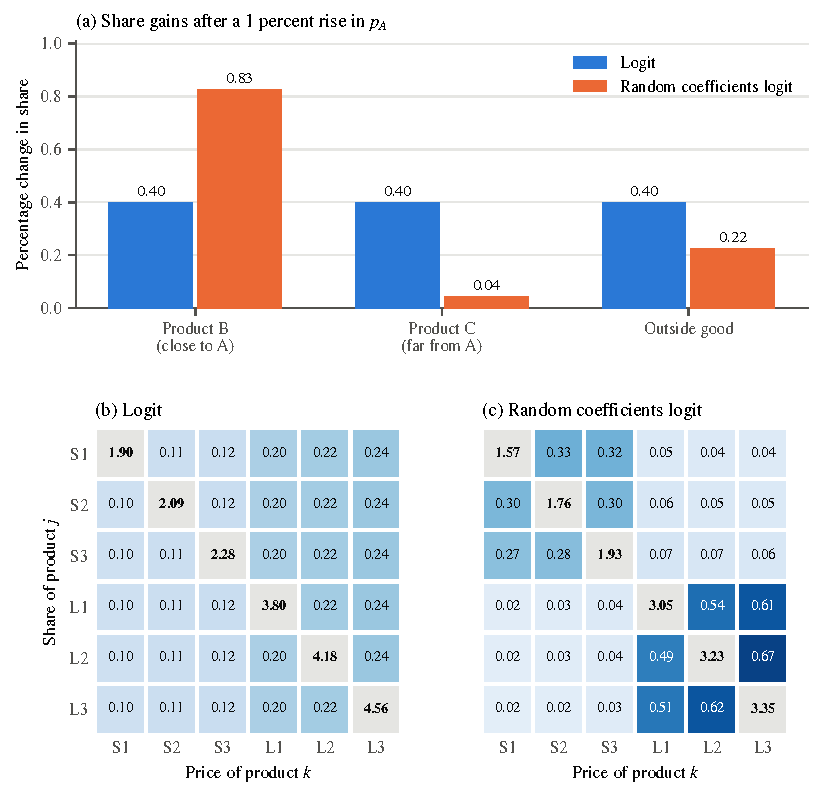
\includegraphics[width=\textwidth]{figures/ch08/fig_substitution.pdf}
\caption{Substitution in the logit and random coefficients logit models. Panel (a): three products with
characteristic $x = (1.0, 0.9, -1.0)$, prices $p = (1, 1, 1)$ and shares $s = (0.20, 0.10, 0.10)$, so A and B are
close and B and C have equal shares. Bars show the percentage change in the shares of B, C and the outside good
after a 1 percent rise in $p_A$. The random coefficients model has normal random coefficients on the constant
(standard deviation 1.0) and on $x$ (standard deviation 2.5), and $\alpha = 2$ in both models. Panels (b) and
(c): six products with shares 0.05, sizes $(-1.0, -0.9, -0.8, 0.8, 0.9, 1.0)$ and prices $(1.0, 1.1, 1.2, 2.0, 2.2,
2.4)$. Cell $(j, k)$ is the elasticity of the share of $j$ with respect to the price of $k$. Grey diagonal cells
report the positive own elasticity $\varepsilon_j = -\varepsilon_{jj}$. The random coefficients model has standard
deviations 1.0 (constant), 2.0 (size) and 0.5 (price), with $\alpha_i = 2 - 0.5\nu_{ip}$. Both models fit the same
shares. Computed by \texttt{figures/ch08/src/fig\_substitution.py}.}
\label{fig:08-substitution}
\end{figure}

\subsection{Further contrasts}\label{sec:08-contrasts}

The vertical model of \cref{ch:discrete} also has heterogeneous consumers, but only along one dimension. Cross
elasticities are then nonzero only between products adjacent in the price ranking.
\citet[p.~852]{BerryLevinsohnPakes1995} give an example. Suppose the ranking contains a \$24,998 family station
wagon, a \$24,999 sports car and a \$25,000 family station wagon, in that order. The vertical model guarantees
that the two wagons are not substitutes for each other, while the sports car is a substitute for both. Random
coefficients on several characteristics let products be differentiated in several dimensions at once.

\begin{remark}[Fitting a logit when tastes are heterogeneous]\label{rem:08-logit-misspec}
Suppose the data come from the random coefficients model and we estimate the logit regression $\ln s_{jt} -
\ln s_{0t} = x_{jt}\beta - \alpha p_{jt} + \text{error}$ by instrumental variables. Write $r_{jt} = \ln s_{jt} -
\ln s_{0t} - \delta_{jt}$ for the gap between the logit inversion and the true mean utility. The regression error is
$\xi_{jt} + r_{jt}$. The gap depends on prices, because less price-sensitive consumers sort into expensive
products. By \eqref{eq:08-elasticity-buyers}, the log share of an expensive product falls with its price at a rate
set by the low price sensitivity of its buyers, more slowly than $\alpha$. An instrument that moves prices, such
as a cost shifter, also moves $r_{jt}$. The instrument is then correlated with the regression error even if it is
independent of $\xi_{jt}$. When less price-sensitive consumers sort into expensive products in this way, the
logit price coefficient tends to be biased toward zero. The argument is heuristic, and \cref{sec:08-worked}
measures the correlation and the bias in a simulated market.
\end{remark}

\begin{remark}[Price changes and product deletions]\label{rem:08-deletion}
\citet[p.~94]{BerryLevinsohnPakes2004} distinguish two substitution patterns. After a price rise, only a selected
group of a product's buyers leave, the more price-sensitive ones. After the product is deleted, all of its buyers
must choose again. The model makes the difference explicit. If $j$ is removed, a consumer who would have bought $j$
chooses $k$ with probability $\frac{s_{ik}}{1 - s_{ij}}$ by \cref{rem:08-iia}. The fraction of $j$'s buyers who move
to $k$ is therefore
\begin{equation}\label{eq:08-deletion-diversion}
  D^{\text{del}}_{jk} = \int \frac{s_{ij}}{s_j}\, \frac{s_{ik}}{1 - s_{ij}}\, \dd F.
\end{equation}
It averages the same individual diversion ratios as \eqref{eq:08-diversion-average}, with weights
$\frac{s_{ij}}{s_j}$ instead of $\varpi_{ij}$. The two coincide in the logit, where both equal $\frac{s_k}{1 -
s_j}$. With heterogeneous tastes they differ, and the deletion pattern is the relevant one for questions such as the
closing of a brand (\cref{sec:08-blp04}).
\end{remark}

\section{Computing the share integral by simulation}\label{sec:08-simulation}

The share integral \eqref{eq:08-share-integral} has the dimension of $(D_i, \nu_i)$, the number of demographics
plus the number of random coefficients. It has no closed form once that dimension exceeds zero, and
\citet[p.~866]{BerryLevinsohnPakes1995} note that numerical integration becomes difficult once the dimension grows
beyond two or three. They replace the integral by a simulation estimator, a technique that
\citet{Pakes1986} introduced as aggregation by simulation \citep[p.~848]{BerryLevinsohnPakes1995}. This section
describes the standard simulator, its error, the importance sampler of \citet{BerryLevinsohnPakes1995}, the
treatment of demographics, deterministic alternatives, and safe numerical evaluation.

\subsection{The smooth simulator}\label{sec:08-smooth-simulator}

Draw $n_s$ consumers $(D_i, \nu_i)$, $i = 1, \dots, n_s$, from $F_{Dt} \times F_\nu$. The \emph{smooth
simulator} of the share of product $j$ is the average of the individual logit probabilities
\citep[eq.~(6.10)]{BerryLevinsohnPakes1995}:
\begin{equation}\label{eq:08-smooth-simulator}
  s^{n_s}_{jt}(\delta_t; \theta_2) = \frac{1}{n_s}\sum_{i=1}^{n_s} s_{ijt}.
\end{equation}
With diagonal $\Sigma$, each term is written out as
\begin{equation*}
  s_{ijt} = \frac{\exp\bigl(\delta_{jt} + \sum_{k} \tilde x_{jtk}(\sigma_k\nu_{ik} + \pi_{k1}D_{i1} + \cdots
            + \pi_{kd}D_{id})\bigr)}
         {1 + \sum_{m \in \mathcal{J}_t}\exp\bigl(\delta_{mt} + \sum_{k} \tilde x_{mtk}(\sigma_k\nu_{ik}
          + \pi_{k1}D_{i1} + \cdots + \pi_{kd}D_{id})\bigr)},
\end{equation*}
which gives equation (11) of \citet{Nevo2000a}. The sums over $k$ run over the characteristics that carry random
coefficients.

The simulator has four properties \citep[p.~865]{BerryLevinsohnPakes1995}. It is unbiased for $s_{jt}$. Its
values are positive. Together with the simulated outside share $\frac{1}{n_s}\sum_i s_{i0t}$ the shares sum to
one. It is a smooth function of $(\delta_t, \theta_2)$. Because the extreme value shocks are integrated
analytically, its variance comes only from the draws of $(D_i, \nu_i)$. The next lemma makes the last point precise
by comparing it with the \emph{frequency simulator}, which also draws the shocks $\epsilon_{ijt}$ and counts the
simulated consumers who choose $j$.

\begin{lemma}[Smooth versus frequency simulator]\label{lem:08-smooth}
Let $s^{\text{freq}}_j = \frac{1}{n_s}\sum_{i=1}^{n_s}\indic\{j = \argmax_{k} u_{ik}\}$, where each simulated
consumer has draws $(D_i, \nu_i, \epsilon_{i0}, \dots, \epsilon_{iJ})$. Both simulators are unbiased for $s_j$, and
\begin{equation}\label{eq:08-rao-blackwell}
  \Var\bigl(s^{\text{freq}}_j\bigr) = \frac{s_j(1 - s_j)}{n_s}
  = \Var\bigl(s^{n_s}_j\bigr) + \frac{1}{n_s}\E\bigl[s_{ij}(1 - s_{ij})\bigr],
  \qquad \Var\bigl(s^{n_s}_j\bigr) = \frac{\Var(s_{ij})}{n_s}.
\end{equation}
\end{lemma}

\begin{proof}
Let $I_{ij}$ be the indicator that simulated consumer $i$ chooses $j$. Conditional on $(D_i, \nu_i)$, it is a
Bernoulli variable with mean $s_{ij}$. By the law of iterated expectations, $\E[I_{ij}] = \E[s_{ij}] = s_j$, so
both simulators are unbiased. Unconditionally $I_{ij}$ is Bernoulli with mean $s_j$, so $\Var(I_{ij}) = s_j(1 -
s_j)$. The law of total variance gives
\begin{equation*}
  \Var(I_{ij}) = \E\bigl[\Var(I_{ij} \mid D_i, \nu_i)\bigr] + \Var\bigl(\E[I_{ij} \mid D_i, \nu_i]\bigr)
              = \E\bigl[s_{ij}(1 - s_{ij})\bigr] + \Var(s_{ij}).
\end{equation*}
The draws are independent across simulated consumers, so dividing by $n_s$ gives the variances of the two
averages.
\end{proof}

The smooth simulator is the conditional expectation of the frequency simulator given the draws of $(D_i,
\nu_i)$. Conditioning removes the variance $\frac{1}{n_s}\E[s_{ij}(1 - s_{ij})]$. The frequency simulator has two
further defects. It is a step function of $(\delta, \theta_2)$, with zero derivatives almost everywhere and jumps
in between, so gradient-based optimizers cannot use it. It also equals zero with positive probability for small
products, and then $\ln s^{\text{freq}}_j$ is undefined and the share equations cannot be inverted.

\subsection{Simulation error in log shares}\label{sec:08-simbias}

The estimator of \cref{sec:08-gmm} uses the simulated shares through their logarithms, in the inversion step. An
unbiased simulator of $s_j$ is a biased simulator of $\ln s_j$. Let $c_j = \frac{\sqrt{\Var(s_{ij})}}{s_j}$ be the
coefficient of variation of the individual purchase probabilities of product $j$.

\begin{proposition}[Bias of the simulated log share]\label{prop:08-simbias}
Let $s^{n_s}_j$ be the smooth simulator with independent draws, and suppose $\Var(s_{ij}) > 0$.
\begin{enumerate}[label=(\roman*)]
  \item $\E[s^{n_s}_j] = s_j$ and $\Var(s^{n_s}_j) = \frac{\Var(s_{ij})}{n_s}$.
  \item $\E[\ln s^{n_s}_j] < \ln s_j$.
  \item If $s_{ij} \ge \underline{s} > 0$ for all $(D_i, \nu_i)$, then
    \begin{equation}\label{eq:08-simbias}
      \E\bigl[\ln s^{n_s}_j\bigr] - \ln s_j = -\frac{\Var(s^{n_s}_j)}{2s_j^2} + O\bigl(n_s^{-\frac{3}{2}}\bigr)
      = -\frac{c_j^2}{2n_s} + O\bigl(n_s^{-\frac{3}{2}}\bigr).
    \end{equation}
\end{enumerate}
\end{proposition}

\begin{proof}
Part (i) restates \cref{lem:08-smooth}. For (ii), the logarithm is strictly concave and $s^{n_s}_j$ is not
degenerate because $\Var(s_{ij}) > 0$. Jensen's inequality gives $\E[\ln s^{n_s}_j] < \ln\E[s^{n_s}_j] = \ln s_j$.

For (iii), write $Y = s^{n_s}_j$ and expand $\ln Y$ around $s_j$ with the Lagrange form of the remainder:
\begin{equation*}
  \ln Y = \ln s_j + \frac{Y - s_j}{s_j} - \frac{(Y - s_j)^2}{2s_j^2} + \frac{(Y - s_j)^3}{3\bar Y^3},
\end{equation*}
where $\bar Y$ lies between $Y$ and $s_j$. Take expectations. The linear term has mean zero by (i). The quadratic
term has mean $-\frac{\Var(Y)}{2s_j^2}$. Both $Y$ and $s_j$ are at least $\underline{s}$, so $\bar Y \ge
\underline{s}$ and the remainder is bounded in absolute value by $\frac{\E|Y - s_j|^3}{3\underline{s}^3}$. For an
average of $n_s$ independent bounded variables, $\E|Y - s_j|^3 \le (\E(Y - s_j)^4)^{\frac{3}{4}}$, and the fourth
central moment of such an average is $O(n_s^{-2})$. The remainder is therefore $O(n_s^{-\frac{3}{2}})$.
Substituting $\Var(Y) = \frac{\Var(s_{ij})}{n_s}$ gives the second form.
\end{proof}

The lower bound in (iii) holds when the support of $(D_i, \nu_i)$ is bounded. With normal tastes it fails, but the
second-order term still describes the bias well in practice, as the evidence below shows. The bias is of order
$\frac{1}{n_s}$ and its size is governed by $c_j$. The coefficient of variation is large when the purchase
probability of $j$ is concentrated on a small group of consumers. Small niche products have the largest $c_j$ and
the largest bias.

The bias passes to the mean utilities. For given $\theta_2$, the inversion of \cref{sec:08-inversion} finds the
$\hat\delta_t$ that solves $s^{n_s}_t(\hat\delta_t; \theta_2) = s^{\text{obs}}_t$. A first-order expansion around
the true $\delta_t$, using the nonsingular Jacobian of \cref{prop:08-shares}, gives
\begin{equation}\label{eq:08-delta-error}
  \hat\delta_t - \delta_t \approx -\Bigl[\frac{\partial s_t}{\partial \delta_t^\T}\Bigr]^{-1}
  \bigl(s^{n_s}_t(\delta_t; \theta_2) - s_t(\delta_t; \theta_2)\bigr).
\end{equation}
The leading term has mean zero and variance of order $\frac{1}{n_s}$. This is the simulation component of the
asymptotic variance of the estimator in \cref{sec:08-gmm}, which \citet[p.~859]{BerryLevinsohnPakes1995} call
$V_3$. The second-order terms, like those in \eqref{eq:08-simbias}, add a bias of order $\frac{1}{n_s}$. At the
true $\delta_t$ the simulated log shares are too low on average, so the inversion tends to push $\hat\delta_t$
up, most for products with dispersed purchase probabilities.

The bias has a consequence for estimation that the variance does not have. Independent draws across markets make
the leading simulation errors independent across markets. They average out of the sample moments as the number of
markets grows. The bias of order $\frac{1}{n_s}$ is present in every market with the same sign, and it does not
average out. Consistency therefore requires $n_s$ to grow with the sample. \citet[p.~859]{BerryLevinsohnPakes1995} cite asymptotic
results of Berry and Pakes, then in progress, for their utility specification. These results require the number
of consumers and the number of simulation draws to grow at the rate $J^3$.
\citet{BerryLintonPakes2004} develop limit theorems of this kind for asymptotics in the number of products.
\citet[Section~4.4]{BerryPakes2007} report the rates that these theorems require. The number of draws must grow at
the slower rate $J^2$ in logit-style models and at rate $J$ in the vertical model (\cref{sec:08-pcm}). BLP's
rate refers to their own utility specification and to results that were still in progress.

\Cref{fig:08-simerror} and \cref{tab:08-simdelta} quantify these effects in one simulated market with five inside
products, shares $(0.10, 0.05, 0.03, 0.015, 0.005)$ and an outside share of 0.80. The market has normal random
coefficients on a constant, a characteristic and price. The coefficients of variation $c_j$ are 1.49, 0.97, 0.94,
1.51 and 2.99. The product with share 0.10 is expensive and bought mostly by consumers who like its
characteristics, so its $c_j$ exceeds those of the two middle products.

\begin{figure}[htbp]
\centering
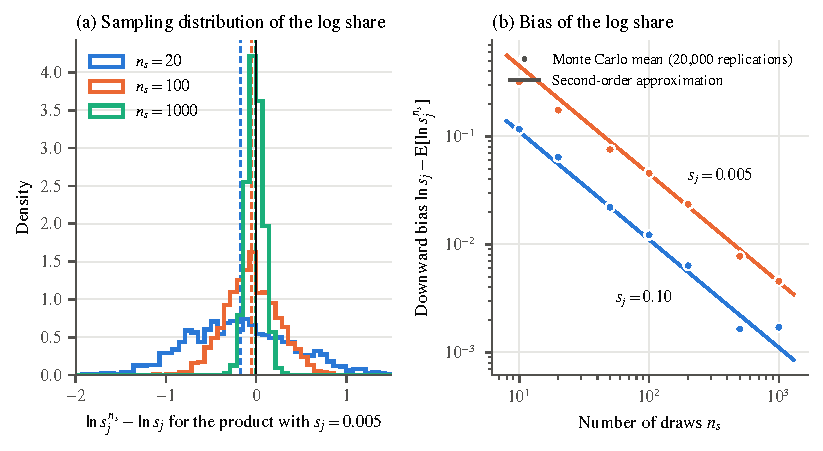
\includegraphics[width=\textwidth]{figures/ch08/fig_simulation.pdf}
\caption{Simulation error in simulated log shares, for one market with outside share 0.80 and inside shares
$(0.10, 0.05, 0.03, 0.015, 0.005)$. Tastes are normal with standard deviations 1.0 on the constant, 1.5 on a characteristic $x =
(1.0, 0.5, 0.0, -0.5, -1.0)$ and 0.5 on price, prices are $(2.0, 1.6, 1.2, 1.0, 0.8)$ and $\alpha = 2$. True shares
come from a 64,000-node Gauss-Hermite rule and agree with $10^6$ pseudo-random draws to within 0.002 in relative
terms. Panel (a): distribution of $\ln s^{n_s}_j - \ln s_j$ for the product with share 0.005 over 2,000 replications
with fresh pseudo-random draws. Dashed lines mark the means. Panel (b): downward bias of the simulated log share
(dots, 20,000 replications per $n_s$) and the second-order approximation $\frac{\Var(s_{ij})}{2n_s s_j^2}$ of
\cref{prop:08-simbias} (lines). Computed by \texttt{figures/ch08/src/fig\_simulation.py}.}
\label{fig:08-simerror}
\end{figure}

Panel (a) of \cref{fig:08-simerror} shows the sampling distribution of the simulated log share of the smallest
product. With 20 draws it is wide and skewed to the left, and its mean lies well below zero. With 1,000 draws it is
concentrated near zero. Panel (b) shows that the downward bias falls like $\frac{1}{n_s}$. The second-order
approximation is accurate from about 50 draws for the product with share 0.10 and from about 100 draws for the
product with share 0.005. For the product with share 0.005, the bias is 0.175
with 20 draws (approximation 0.224), 0.046 with 100 draws (approximation 0.045), and 0.005 with 1,000 draws
(approximation 0.004). With 10 or 20 draws the approximation overstates the bias of the smallest product, because
higher-order terms matter when the simulator is very noisy.

\begin{table}[htbp]
\centering
\caption{Error in the inverted mean utility caused by simulation}\label{tab:08-simdelta}
\begin{tabular}{lccccc}
\toprule
 & \multicolumn{5}{c}{Market share of the product} \\
\cmidrule(lr){2-6}
Draws $n_s$ & 0.10 & 0.05 & 0.03 & 0.015 & 0.005 \\
\midrule
20    & 0.037 & 0.010 & 0.021 & 0.063 & 0.198 \\
      & (0.547) & (0.362) & (0.273) & (0.368) & (0.627) \\
100   & $-0.008$ & $-0.009$ & $-0.008$ & $-0.006$ & 0.015 \\
      & (0.250) & (0.163) & (0.126) & (0.177) & (0.328) \\
1,000 & 0.003 & 0.001 & $-0.000$ & $-0.002$ & $-0.006$ \\
      & (0.077) & (0.051) & (0.040) & (0.056) & (0.104) \\
\bottomrule
\end{tabular}

\smallskip
\begin{minipage}{0.86\linewidth}
\footnotesize Notes: Each entry is the mean of $\hat\delta_j - \delta_j$ over 500 replications, with its standard
deviation in parentheses. In each replication we draw $n_s$ consumers and solve $s^{n_s}(\hat\delta; \theta_2) =
s$ by the contraction of \cref{sec:08-inversion}, at the true $\theta_2$ and the true shares. The market is the one
of \cref{fig:08-simerror}. The standard error of each mean is its standard deviation divided by
$\sqrt{500} \approx 22.4$. Computed by \texttt{figures/ch08/src/fig\_simulation.py}.
\end{minipage}
\end{table}

\Cref{tab:08-simdelta} turns to the mean utilities. With 20 draws, the inverted $\hat\delta_j$ of the product
with share 0.005 is too high by 0.198 on average, with a standard error of $\frac{0.627}{22.4} = 0.028$. The
product with share 0.015 is too high by 0.063 (standard error 0.016). These are the upward biases predicted
above. Their size is small relative to the standard deviations, which range from 0.27 to 0.63. The standard
deviations fall roughly like $\frac{1}{\sqrt{n_s}}$, from about 0.4 on average with 20 draws to about 0.07 with
1,000 draws. With 100 or more draws the mean errors are within two standard errors of zero.

\subsection{Draws in practice}\label{sec:08-draws}

Three rules govern the use of simulation draws in estimation.

The draws are taken once, before estimation, and held fixed while the optimizer varies the parameters. If new
draws were taken at each evaluation, the objective would be a different random function each time it is
evaluated. The search would chase the simulation noise and fail to converge. The asymptotic theory of simulation
estimators also requires draws that do not change with $\theta$ \citep[p.~867]{BerryLevinsohnPakes1995},
\citep{PakesPollard1989}.

Draws are usually independent across markets. Then simulation errors are independent across markets and their
leading terms average out of the moments, so a moderate number of draws per market can suffice when markets are
many. The bias term of \cref{prop:08-simbias} is the exception, as explained above. \citet{BerryLevinsohnPakes1995}
instead hold the same draws of $(\nu_{iy}, \nu_{i0}, \dots, \nu_{iK})$ fixed over all years of their panel, while the
income distribution shifts through $m_t$ \citep[p.~868]{BerryLevinsohnPakes1995}.

The number of draws trades accuracy against computing time. \citet[pp.~538, 540]{Nevo2000a} draws 20 consumers per market
in his illustrative application and notes that more draws or better simulation methods would improve efficiency.
The evidence above shows that 20 pseudo-random draws leave sizable errors in the shares of small products.

Demographics need their own draws. \citet[p.~868, n.~21]{BerryLevinsohnPakes1995} tried taking draws of income from the
CPS for each year. They found that this less restrictive procedure gave imprecise simulators, in particular for
changes in the upper tail of the income distribution. They therefore kept a lognormal income distribution with
year-specific means. They did not estimate a separate standard deviation for each year because those estimates were
imprecise. \citet[n.~25]{Nevo2001} samples 40 individuals from the CPS for each city and year, 200 for each city in
total. He reports that the results were robust to increasing the number of individuals where possible. Empirical
draws of $D_i$ are combined with independent draws of $\nu_i$ from $F_\nu$.

\subsection{Importance sampling}\label{sec:08-importance}

Pseudo-random draws from $F_\nu$ waste effort when few consumers buy any inside product. In the car market most
households do not buy a new car in a given year. Most draws then have purchase probabilities near zero and
contribute little to any share. \citet[Section~6.3]{BerryLevinsohnPakes1995} reduce the variance of the simulator by
importance sampling. To keep notation light, let $\nu$ collect all simulated consumer characteristics, with density
$p_0(\nu)$, and write $f_j(\nu, \theta)$ for the individual choice probability \eqref{eq:08-individual-share}.

Take any density $h(\nu, \theta)$ that is positive wherever $p_0$ is. The share can be rewritten as
\citep[eq.~(6.11)]{BerryLevinsohnPakes1995}
\begin{equation}\label{eq:08-importance-identity}
  s_j(\theta) = \int f_j(\nu, \theta)\, p_0(\nu)\, \dd\nu
  = \int \Bigl[\frac{f_j(\nu, \theta)\, p_0(\nu)}{h(\nu, \theta)}\Bigr] h(\nu, \theta)\, \dd\nu.
\end{equation}
Averaging the bracketed term over draws from $h$ gives an unbiased simulator. Its variance is the variance of the
bracketed term under $h$, divided by the number of draws. The variance is zero for the choice
\citep[eq.~(6.12)]{BerryLevinsohnPakes1995}
\begin{equation}\label{eq:08-optimal-importance}
  h^*_j(\nu, \theta) = \frac{f_j(\nu, \theta)\, p_0(\nu)}{s_j(\theta)},
\end{equation}
because the bracketed term then equals $s_j(\theta)$ for every draw. This density over-samples consumers whose
characteristics make them likely to buy product $j$.

The optimal density cannot be used directly, for three reasons \citep[pp.~866--867]{BerryLevinsohnPakes1995}. It
requires $s_j(\theta)$, the integral we want to compute. It depends on $\theta$, while the draws must stay fixed as
the optimizer varies $\theta$. It differs across products, so each simulated share would come from its own draws.
The inversion of \cref{sec:08-inversion} instead computes all shares from one distribution of consumers.

\citeauthor{BerryLevinsohnPakes1995} build a feasible version from a preliminary estimate $\theta'$, obtained with the
smooth simulator. They target the probability of buying some car, $\bar f(\nu, \theta') = \sum_{j=1}^{J} f_j(\nu,
\theta')$, whose integral is the total inside share $\bar s(\theta') = 1 - s_0(\theta')$. Draws come from $p_0$ by
acceptance and rejection: a draw $\nu$ is accepted with probability $\bar f(\nu, \theta')$. By Bayes' rule the
density of an accepted draw is
\begin{equation}\label{eq:08-accepted-density}
  h(\nu) = \frac{p_0(\nu)\, \Pr(\text{accept} \mid \nu)}{\Pr(\text{accept})}
         = \frac{p_0(\nu)\, \bar f(\nu, \theta')}{\int p_0(\nu')\, \bar f(\nu', \theta')\, \dd\nu'}
         = \frac{p_0(\nu)\, \bar f(\nu, \theta')}{\bar s(\theta')}.
\end{equation}
Substituting this $h$ into \eqref{eq:08-importance-identity} gives the bracketed term $\frac{\bar
s(\theta')}{\bar f(\nu, \theta')}f_j(\nu, \theta)$. With $n_s$ accepted draws $\nu_1, \dots, \nu_{n_s}$, the
simulator is \citep[eq.~(6.13)]{BerryLevinsohnPakes1995}\footnote{Equation (6.13) of
\citet{BerryLevinsohnPakes1995} is printed without the factor $\frac{1}{n_s}$. The average is needed for the
simulator to be unbiased.}
\begin{equation}\label{eq:08-blp-importance}
  s_j\bigl[\theta, P^*_h(\theta')_{n_s}\bigr] = \frac{1}{n_s}\sum_{i=1}^{n_s}
  \frac{\bar s(\theta')}{\bar f(\nu_i, \theta')}\, f_j(\nu_i, \theta).
\end{equation}
The draws are fixed once $\theta'$ is chosen, and every share uses the same draws. Since $\bar s(\theta')$ is computed
only once, it can be computed with many draws at little cost.

The construction removes one source of noise. At $\theta = \theta'$ the weighted integrand is $\bar s(\theta')$ times
$\frac{f_j(\nu, \theta')}{\bar f(\nu, \theta')}$, the probability of choosing $j$ given that the consumer buys some
car. That ratio lies between zero and one. Summed over $j$ it equals $\bar s(\theta')$ for every draw, so the
simulated total inside share has no simulation error at all. The variation that remains comes only from which car
a buyer chooses.

Common draws do not make the simulated shares add up to one, although \citet[p.~867]{BerryLevinsohnPakes1995} use
them for that purpose. Write $w_i = \frac{\bar s(\theta')}{\bar f(\nu_i, \theta')}$ for the weight of draw $i$ and
$\bar w = \frac{1}{n_s}\sum_{i} w_i$ for the mean weight. Applying \eqref{eq:08-blp-importance} to all $J + 1$
options and using $\sum_{j=0}^{J} f_j = 1$ gives $\sum_{j=0}^{J} s_j = \bar w$. Each weight has expectation one under
$h$, so $\bar w$ equals one only on average. The contraction uses only the inside shares, and this random total does
not break it. The simulated inside shares equal $\bar w$ times the shares computed under the probability weights
$\frac{w_i}{n_s\bar w}$. \Cref{thm:08-berry94}, applied to this distribution of draws, gives a unique solution
whenever the observed inside shares sum to less than $\bar w$. With a small inside share and many draws, $\bar w$ is
close to one and the condition is mild. Self-normalizing the weights would make the shares sum to one exactly, at
the cost of a finite-sample bias that vanishes as $n_s$ grows.

\Cref{tab:08-importance} compares the two simulators in the market of \cref{fig:08-simerror}, whose total inside share
is 0.20. With 100 draws, importance sampling cuts the relative root mean squared error of the largest product's share
from 15.3 to 4.8 percent. For the second product it falls from 10.0 to 2.8 percent. The gains are small for
the two smallest products, from 15.0 to 13.5 percent and from 29.4 to 25.5 percent. Their buyers are a small subset of
car buyers, so conditioning on buying some car leaves most of their simulation noise in place. A preliminary
estimate that understates every standard deviation by 20 percent loses little of the gain.

\begin{table}[htbp]
\centering
\caption{Smooth simulator and importance sampling: relative root mean squared error (percent)}\label{tab:08-importance}
\begin{tabular}{lccccc}
\toprule
 & \multicolumn{5}{c}{Market share of the product} \\
\cmidrule(lr){2-6}
Simulator & 0.10 & 0.05 & 0.03 & 0.015 & 0.005 \\
\midrule
Smooth simulator & 15.31 & 9.95 & 9.52 & 14.98 & 29.35 \\
Importance sampling, $\theta' = \theta$ & 4.83 & 2.84 & 6.79 & 13.51 & 25.46 \\
Importance sampling, $\sigma' = 0.8\sigma$ & 5.55 & 2.90 & 6.35 & 13.28 & 26.31 \\
\bottomrule
\end{tabular}

\smallskip
\begin{minipage}{0.9\linewidth}
\footnotesize Notes: Each entry is $100\sqrt{\E\bigl[(\frac{\hat s_j}{s_j} - 1)^2\bigr]}$ over 1,000 replications
with $n_s = 100$ draws (accepted draws for importance sampling). The importance sampler is
\eqref{eq:08-blp-importance}. In the last row the preliminary estimate $\theta'$ multiplies every standard deviation by
0.8 and uses the mean utilities that fit the shares at those values. The acceptance rate equals the total inside share,
0.20. Mean errors of the importance sampler are below 0.6 percent in absolute value. Computed by
\texttt{figures/ch08/src/fig\_simulation.py}.
\end{minipage}
\end{table}

\subsection{Quadrature and quasi-Monte Carlo}\label{sec:08-quadrature}

Pseudo-random draws are not the only way to approximate \eqref{eq:08-share-integral}. Any rule of the form $\sum_q w_q
s_{ij}(\nu_q)$ with nodes $\nu_q$ and weights $w_q$ can replace the simple average, and the share equations and
their inversion are unchanged.

A \emph{Gauss-Hermite product rule} uses, in each dimension, the $Q$ nodes and weights that integrate polynomials of
degree up to $2Q - 1$ exactly against the normal density. For a standard normal variable,
\begin{equation}\label{eq:08-gauss-hermite}
  \int g(\nu)\, \phi(\nu)\, \dd\nu \approx \sum_{q=1}^{Q} \frac{w_q}{\sqrt{\pi}}\, g\bigl(\sqrt{2}\, x_q\bigr),
\end{equation}
where $(x_q, w_q)$ are the Gauss-Hermite nodes and weights for the weight function $e^{-x^2}$. The product rule takes
all combinations of the one-dimensional nodes, so it needs $Q^{L}$ nodes for $L$ random coefficients. It is very
accurate for smooth integrands in low dimensions and becomes expensive quickly as $L$ grows. \emph{Sparse grids}
combine lower-order product rules so that the number of nodes grows polynomially in $L$ \citep{HeissWinschel2008}.
\emph{Quasi-Monte Carlo} methods, such as Halton sequences, replace pseudo-random draws by deterministic sequences that
fill the unit cube more evenly. The points are mapped to normal draws by the inverse distribution function
\citep[Section~9.3.3]{Train2009}.
A randomly scrambled Halton sequence keeps the even coverage and allows replications. The
\texttt{pyblp} software of \citet[Section~3]{ConlonGortmaker2020} implements all of these rules. By default it
scrambles each Halton sequence and discards its first 1,000 points.

\Cref{tab:08-integration} compares the three approaches in the market of \cref{fig:08-simerror}, which has three random
coefficients. At equal numbers of nodes, scrambled Halton draws reduce the error of pseudo-random draws by a factor of
about 2 to 20, and the gain grows with the number of nodes. The Gauss-Hermite product rule is accurate to a few hundredths of a percent with 125 nodes and to about
$10^{-5}$ percent with 1,000 nodes. The product rule's advantage shrinks with more random coefficients. It also shrinks when
demographic distributions are known only through empirical draws, which quadrature cannot use directly.

\begin{table}[htbp]
\centering
\caption{Accuracy of integration rules: relative error of simulated shares (percent)}\label{tab:08-integration}
\begin{tabular}{lccc}
\toprule
 & \multicolumn{3}{c}{Number of nodes} \\
\cmidrule(lr){2-4}
Rule & 125 & 1,000 & 8,000 \\
\midrule
\multicolumn{4}{l}{\textit{Product with $s_j = 0.10$}} \\
Pseudo-random draws & 12.45 & 4.84 & 1.56 \\
Scrambled Halton draws & 3.41 & 0.53 & 0.076 \\
Gauss-Hermite product rule & $2.9 \times 10^{-2}$ & $1.9 \times 10^{-5}$ & $3.0 \times 10^{-10}$ \\
\addlinespace
\multicolumn{4}{l}{\textit{Product with $s_j = 0.005$}} \\
Pseudo-random draws & 27.63 & 10.29 & 3.30 \\
Scrambled Halton draws & 13.38 & 2.45 & 0.46 \\
Gauss-Hermite product rule & $4.5 \times 10^{-2}$ & $2.5 \times 10^{-5}$ & $6.2 \times 10^{-10}$ \\
\bottomrule
\end{tabular}

\smallskip
\begin{minipage}{0.8\linewidth}
\footnotesize Notes: Market of \cref{fig:08-simerror}, with three normal random coefficients. Entries for random rules
are relative root mean squared errors over 200 replications. Entries for the Gauss-Hermite rule, which uses 5, 10 and
20 nodes per dimension, are absolute relative errors against a rule with 40 nodes per dimension. Computed by
\texttt{figures/ch08/src/fig\_simulation.py}.
\end{minipage}
\end{table}

\subsection{Safe numerical evaluation}\label{sec:08-overflow}

Evaluating \eqref{eq:08-individual-share} naively can overflow. Mean utilities and random coefficient terms can be
large during the search, and $e^{V}$ exceeds the largest double-precision number once $V$ exceeds about 709. The
logit formula is invariant to subtracting the same constant from every utility of a consumer, including the zero
utility of the outside good. Let $m_i = \max\{0, \max_k V_{ik}\}$. Then
\begin{equation}\label{eq:08-logsumexp}
  s_{ij} = \frac{e^{V_{ij} - m_i}}{e^{-m_i} + \sum_k e^{V_{ik} - m_i}}, \qquad
  \ln s_{ij} = V_{ij} - m_i - \ln\Bigl(e^{-m_i} + \sum_k e^{V_{ik} - m_i}\Bigr).
\end{equation}
Every exponent is now at most zero, and at least one term in the denominator equals one, so neither overflow nor
division by zero can occur. The second expression, the log-sum-exp form, also gives accurate log shares for very
small probabilities. All computations in this chapter use \eqref{eq:08-logsumexp}.

\section{Inverting the share equations: the BLP contraction}\label{sec:08-inversion}

The model of \cref{sec:08-model} maps mean utilities into market shares. Estimation needs the reverse
map. The reason is that the unobserved quality $\xi_{jt}$ enters the model only through the mean utility
$\delta_{jt} = x_{jt}\beta - \alpha p_{jt} + \xi_{jt}$, and it enters linearly. Suppose we can recover the vector
$\delta_t$ from the observed shares. Then $\xi_{jt}$ becomes a known function of the data and the
parameters, and instrumental variable methods apply as in a linear demand model. \citet[pp.~850--851]%
{BerryLevinsohnPakes1995} make the point directly. The orthogonality between $\xi$ and the instruments
cannot be used ``without first transforming the observed quantity, price, and characteristic data into a
linear function of $\xi$.'' This section shows that the transformation exists, that it is unique, and that a
simple iteration computes it.

\subsection{The inversion problem}\label{sec:08-inv-problem}

Fix the nonlinear parameters $\theta_2 = (\Pi, \Sigma)$ and a market $t$ with $J_t$ inside products. Recall
from \cref{sec:08-model} that the model share of product $j$ is
\begin{equation}\label{eq:08-p2-share}
  s_{jt}(\delta_t;\theta_2) = \int \frac{\exp(\delta_{jt} + \mu_{ijt})}{1 + \sum_{k \in \mathcal{J}_t}
  \exp(\delta_{kt} + \mu_{ikt})}\, \dd F(D_i, \nu_i),
  \qquad \mu_{ijt} = \tilde x_{jt}(\Pi D_i + \Sigma\nu_i),
\end{equation}
where $\tilde x_{jt} = (x_{jt}, p_{jt})$ collects the characteristics that carry random coefficients. We
write $s_{ijt}$ for the integrand, the choice probability of a consumer with attributes $(D_i, \nu_i)$, and
$s_{i0t} = 1 - \sum_{k} s_{ikt}$ for that consumer's probability of choosing the outside good. The
\emph{inversion problem} is to find, for each market, the vector $\delta_t \in \R^{J_t}$ that solves
\begin{equation}\label{eq:08-inv-system}
  s_{jt}(\delta_t;\theta_2) = s^{\text{obs}}_{jt}, \qquad j = 1, \dots, J_t,
\end{equation}
where $s^{\text{obs}}_{jt}$ is the observed share \citep[eq.~10]{Nevo2000a}. The system has $J_t$ equations in
$J_t$ unknowns. Markets separate, because $\delta_t$ affects only the shares of market $t$. We denote the
solution by $\delta_t(s^{\text{obs}}_t;\theta_2)$, or $\delta_t(\theta_2)$ when the data are understood.

In three familiar models the inverse has a closed form. In the logit model $\Pi = \Sigma = 0$, so
$s_{jt} = \frac{e^{\delta_{jt}}}{1 + \sum_k e^{\delta_{kt}}}$ and $s_{0t} = \frac{1}{1 + \sum_k
e^{\delta_{kt}}}$. Dividing,
\begin{equation*}
  \frac{s_{jt}}{s_{0t}} = e^{\delta_{jt}},
\end{equation*}
and taking logarithms gives
\begin{equation}\label{eq:08-logit-inv}
  \delta_{jt} = \ln s^{\text{obs}}_{jt} - \ln s^{\text{obs}}_{0t},
\end{equation}
which is equation (6.4) of \citet{BerryLevinsohnPakes1995}. In the nested logit model with nesting
parameter $\sigma$ the same algebra applied within and across nests gives $\delta_{jt} = \ln s_{jt} - \ln
s_{0t} - \sigma\ln s_{j|g,t}$, where $s_{j|g,t}$ is the share of $j$ within its nest $g$ \citep{Berry1994}.
\Cref{ch:logit} derives this formula. The principles of differentiation generalized extreme value (PD-GEV) model of
\citet{BresnahanSternTrajtenberg1997} also has an analytic inverse \citep[p.~532]{Nevo2000a}. In each case
the ratios of shares isolate $\delta_{jt}$ because the shares have a closed form. Random coefficients
destroy the closed form, since \eqref{eq:08-p2-share} is an integral. The inverse must then be computed
numerically, and this must be done again for every trial value of $\theta_2$.

Two features of \eqref{eq:08-inv-system} matter for what follows. First, the observed shares appear on the
right-hand side. The inversion therefore fits the observed shares exactly, and all discrepancies between
model and data are attributed to $\xi_{jt}$. Second, the logit inversion \eqref{eq:08-logit-inv} is the
exact solution when $\theta_2 = 0$. It is the natural starting value for the numerical methods below.

\subsection{Existence and uniqueness}\label{sec:08-inv-existence}

The first question is whether \eqref{eq:08-inv-system} has a solution and whether the solution is unique.
\citet[p.~249 and Appendix]{Berry1994} answered both questions for a general family of discrete choice
models. \citet[Appendix I]{BerryLevinsohnPakes1995} gave a second proof that also delivers an algorithm.
We state the result for the random coefficients logit model and prove it through the BLP route.

\begin{theorem}[Invertibility of the share system]\label{thm:08-berry94}
Fix $\theta_2$ and a market $t$. Suppose the distribution $F$ of $(D_i, \nu_i)$ satisfies
$\int e^{\mu_{ijt}}\, \dd F < \infty$ for every $j$. Then for every vector $s = (s_1, \dots, s_{J_t})$ with
$s_j > 0$ for all $j$ and $\sum_j s_j < 1$, there is exactly one $\delta \in \R^{J_t}$ such that
$s_t(\delta;\theta_2) = s$. Moreover, a truncated version of the iteration $\delta \mapsto \delta + \ln s -
\ln s_t(\delta;\theta_2)$ converges to this $\delta$ from any starting value.
\end{theorem}

The integrability condition holds in the usual specifications. With normal taste shocks and demographics
of bounded support, $\int e^{\mu_{ijt}}\, \dd F$ is a moment generating function evaluated at a finite point.
The proof rests on an abstract fixed point theorem, which we state and prove first.

\begin{theorem}[\citealp{BerryLevinsohnPakes1995}, Appendix I]\label{thm:08-contraction}
Consider $\R^{J}$ with the sup norm $\Vert y \Vert = \max_j |y_j|$. Let $f: \R^J \to \R^J$ satisfy the
following conditions.
\begin{enumerate}[label=(\arabic*)]
  \item $f$ is continuously differentiable. For all $j$ and $k$ and all $y$, $\frac{\partial f_j(y)}{\partial
  y_k} \geq 0$ and $\sum_{k=1}^{J}\frac{\partial f_j(y)}{\partial y_k} < 1$.
  \item $f$ is bounded below: $\min_j \inf_y f_j(y) \equiv \underline{y} > -\infty$.
  \item There is a value $\bar y$ with the following property. If $y_j \geq \bar y$ for some $j$, then
  $f_k(y) < y_k$ for some $k$ (not necessarily equal to $j$).
\end{enumerate}
Then $f$ has a unique fixed point $y^*$ in $\R^J$. Moreover, let $Y = [\underline y, \bar y]^J$ and define the
truncated map $\hat f: \R^J \to Y$ by $\hat f_j(y) = \min\{f_j(y), \bar y\}$. Then $\hat f$ is a contraction on
$Y$ with modulus strictly less than one, and the iterates $\hat f^{\,h}(y)$ converge to $y^*$ from any
$y \in \R^J$.
\end{theorem}

\begin{proof}
If condition (3) holds for $\bar y$, it holds for every larger value. We may therefore assume $\bar y >
\underline y$. The proof has four steps.

\emph{Step 1.} We show that $\hat f$ maps $\R^J$ into $Y$. For any $y$, $\hat f_j(y) \leq \bar y$ by construction. Also
$f_j(y) \geq \underline y$ by condition (2), so $\hat f_j(y) \geq \min\{\underline y, \bar y\} =
\underline y$.

\emph{Step 2.} We show that $\hat f$ is a contraction on $Y$. Take $y, y' \in Y$ and let $\lambda = \Vert y - y'\Vert$.
Write $\mathbf{1}$ for the vector of ones, so that $y + \lambda\mathbf{1} \geq y'$ element by element. Fix a
component $j$ and assume without loss of generality that $\hat f_j(y') \geq \hat f_j(y)$. If $f_j(y) \geq
\bar y$, then $\hat f_j(y) = \bar y \geq \hat f_j(y')$, so $\hat f_j(y') - \hat f_j(y) = 0$. Otherwise
$\hat f_j(y) = f_j(y)$. Condition (1) makes $f_j$ nondecreasing in every argument, and taking the minimum
with a constant preserves this. Hence
\begin{align*}
  0 \leq \hat f_j(y') - \hat f_j(y)
  &\leq \hat f_j(y + \lambda\mathbf{1}) - \hat f_j(y) \\
  &\leq f_j(y + \lambda\mathbf{1}) - f_j(y) \\
  &= \int_0^{\lambda}\sum_{k=1}^{J}\frac{\partial f_j(y + z\mathbf{1})}{\partial y_k}\, \dd z.
\end{align*}
The first inequality uses monotonicity and $y' \leq y + \lambda\mathbf{1}$. The second uses
$\hat f_j \leq f_j$ and $\hat f_j(y) = f_j(y)$. The equality is the fundamental theorem of calculus applied to
$z \mapsto f_j(y + z\mathbf{1})$, with the chain rule. Now define the compact set
\begin{equation*}
  \mathcal{W} = \{y + z\mathbf{1}: y \in Y,\ z \in [0, \bar y - \underline y]\}
\end{equation*}
and the number
\begin{equation*}
  \kappa = \max_j \max_{w \in \mathcal{W}} \sum_{k=1}^{J}\frac{\partial f_j(w)}{\partial y_k}.
\end{equation*}
The maximum exists because the row sum is continuous and $\mathcal{W}$ is compact. Each row sum is below
one at every point, so $\kappa < 1$. Since $y, y' \in Y$, we have $\lambda \leq \bar y - \underline y$, so
every point $y + z\mathbf{1}$ with $z \in [0, \lambda]$ lies in $\mathcal{W}$. The integrand is therefore at
most $\kappa$, and
\begin{equation*}
  |\hat f_j(y') - \hat f_j(y)| \leq \kappa\lambda = \kappa\Vert y' - y\Vert.
\end{equation*}
This holds for every $j$, so $\Vert \hat f(y') - \hat f(y)\Vert \leq \kappa \Vert y' - y\Vert$.

\emph{Step 3.} We show that the fixed point of $\hat f$ is a fixed point of $f$. The set $Y$ is closed, hence complete. By
the contraction mapping theorem (\cref{app:math}), $\hat f$ has a unique fixed point $y^*$ in $Y$. By Step 1
the iterates from any starting value enter $Y$ after one step, and they then converge to $y^*$. Suppose some
component satisfies $y^*_j = \bar y$. Condition (3) gives an index $k$ with $f_k(y^*) < y^*_k$. Then $\hat
f_k(y^*) \leq f_k(y^*) < y^*_k$, which contradicts $\hat f(y^*) = y^*$. Hence $y^*_j < \bar y$ for all $j$.
For each $j$, $\hat f_j(y^*) = y^*_j < \bar y$ forces $\hat f_j(y^*) = f_j(y^*)$. So $f(y^*) = y^*$.

\emph{Step 4.} We show that $f$ has no other fixed point. Let $f(y) = y$ for some $y \in \R^J$. Condition (2) gives $y_j
= f_j(y) \geq \underline y$ for all $j$. If $y_j \geq \bar y$ for some $j$, condition (3) gives $k$ with
$f_k(y) < y_k$, a contradiction. So $y \in Y$ and $y_j < \bar y$ for all $j$, which gives $\hat f(y) = f(y) =
y$. Uniqueness of the fixed point of $\hat f$ on $Y$ then yields $y = y^*$.
\end{proof}

\Citet[p.~887]{BerryLevinsohnPakes1995} note that the proof imposes the upper bound $\bar y$, ``although in
practice we never had to impose this bound.'' The truncation is a device of the proof. We now apply the
theorem to the map
\begin{equation}\label{eq:08-phi}
  \Phi_t(\delta_t) = \delta_t + \ln s^{\text{obs}}_t - \ln s_t(\delta_t;\theta_2),
\end{equation}
defined element by element. A vector $\delta_t$ is a fixed point of $\Phi_t$ exactly when it solves
\eqref{eq:08-inv-system}. The next result supplies condition (1).

\begin{corollary}[Derivatives of the BLP map]\label{cor:08-rowsum}
In the random coefficients logit model, for all $j$ and all $k \neq j$,
\begin{equation*}
  \frac{\partial \Phi_{jt}}{\partial \delta_{jt}} = \frac{1}{s_{jt}}\int s_{ijt}^2\, \dd F > 0, \qquad
  \frac{\partial \Phi_{jt}}{\partial \delta_{kt}} = \frac{1}{s_{jt}}\int s_{ijt}s_{ikt}\, \dd F > 0,
\end{equation*}
and the row sums satisfy
\begin{equation}\label{eq:08-rowsum}
  \sum_{k \in \mathcal{J}_t}\frac{\partial \Phi_{jt}}{\partial \delta_{kt}} = 1 -
  \frac{1}{s_{jt}}\int s_{ijt}s_{i0t}\, \dd F = 1 - \int s_{i0t}\,\frac{s_{ijt}}{s_{jt}}\, \dd F \in (0,1).
\end{equation}
\end{corollary}

\begin{proof}
Drop the market index. Write $V_{ij} = \delta_j + \mu_{ij}$, so that $s_{ij} = \frac{e^{V_{ij}}}{1 +
\sum_m e^{V_{im}}}$. The quotient rule gives the individual derivatives
\begin{equation*}
  \frac{\partial s_{ij}}{\partial \delta_j} = s_{ij}(1 - s_{ij}), \qquad
  \frac{\partial s_{ij}}{\partial \delta_k} = -s_{ij}s_{ik} \quad (k \neq j).
\end{equation*}
These derivatives are bounded by one in absolute value, so we may differentiate \eqref{eq:08-p2-share}
under the integral sign by dominated convergence (\cref{prop:08-shares}). This gives
$\frac{\partial s_j}{\partial \delta_j} = \int s_{ij}(1 - s_{ij})\, \dd F$ and $\frac{\partial s_j}{\partial
\delta_k} = -\int s_{ij}s_{ik}\, \dd F$. Differentiating \eqref{eq:08-phi},
\begin{equation*}
  \frac{\partial \Phi_j}{\partial \delta_j} = 1 - \frac{1}{s_j}\frac{\partial s_j}{\partial \delta_j}
  = 1 - \frac{1}{s_j}\int s_{ij}\, \dd F + \frac{1}{s_j}\int s_{ij}^2\, \dd F
  = \frac{1}{s_j}\int s_{ij}^2\, \dd F,
\end{equation*}
because $\int s_{ij}\, \dd F = s_j$. For $k \neq j$, $\frac{\partial \Phi_j}{\partial \delta_k} =
-\frac{1}{s_j}\frac{\partial s_j}{\partial \delta_k} = \frac{1}{s_j}\int s_{ij}s_{ik}\, \dd F$. Both are
positive since $s_{ij} \in (0,1)$. Summing over $k$,
\begin{equation*}
  \sum_k \frac{\partial \Phi_j}{\partial \delta_k} = \frac{1}{s_j}\int s_{ij}\Big(s_{ij} + \sum_{k \neq
  j}s_{ik}\Big)\, \dd F = \frac{1}{s_j}\int s_{ij}(1 - s_{i0})\, \dd F = 1 - \frac{1}{s_j}\int s_{ij}s_{i0}\,
  \dd F.
\end{equation*}
The last integral is positive and smaller than $s_j$, so the row sum lies in $(0,1)$.
\end{proof}

The identity $\sum_k \frac{\partial s_{ij}}{\partial \delta_k} = s_{ij}s_{i0}$, used implicitly in the
proof, has a simple reading. Raising every inside mean utility by the same amount is equivalent to lowering
the utility of the outside good. It moves consumers of type $i$ from the outside good to $j$ at the rate
$s_{ij}s_{i0}$.

\begin{proof}[Proof of \cref{thm:08-berry94}]
We verify the three conditions of \cref{thm:08-contraction} for $f = \Phi$ with $\ln s^{\text{obs}}$ replaced by
$\ln s$, dropping the market index.

\emph{Condition (1).} The share function is infinitely differentiable (\cref{prop:08-shares}), so $\Phi$ is
continuously differentiable. \Cref{cor:08-rowsum} gives nonnegative partial derivatives and row sums below
one.

\emph{Condition (2).} Write $s_j(\delta) = e^{\delta_j}B_j(\delta)$, with
\begin{equation*}
  B_j(\delta) = \int \frac{e^{\mu_{ij}}}{1 + \sum_k e^{\delta_k + \mu_{ik}}}\, \dd F.
\end{equation*}
Then $\Phi_j(\delta) = \delta_j + \ln s_j - \delta_j - \ln B_j(\delta) = \ln s_j - \ln B_j(\delta)$. The
function $B_j$ falls in every $\delta_k$ and is bounded above by $\int e^{\mu_{ij}}\, \dd F$, its limit
when all $\delta_k \to -\infty$. Hence
\begin{equation*}
  \Phi_j(\delta) \geq \underline\delta_j \equiv \ln s_j - \ln\int e^{\mu_{ij}}\, \dd F,
\end{equation*}
which is finite by the integrability assumption. Set $\underline y = \min_j \underline\delta_j$
\citep[p.~888]{BerryLevinsohnPakes1995}. The bound $\underline\delta_j$ is the mean utility that would
generate share $s_j$ if every consumer's denominator in \eqref{eq:08-p2-share} were equal to one.

\emph{Condition (3).} We follow \citet[p.~261]{Berry1994}. For each $j$, consider the market in which only
product $j$ is available, so that the outside share is $s_0^{(j)}(\delta_j) = \int \frac{1}{1 + e^{\delta_j
+ \mu_{ij}}}\, \dd F$. This function is continuous and strictly decreasing, with limits one and zero as
$\delta_j \to -\infty$ and $\delta_j \to +\infty$. Let $\bar\delta_j$ solve $s_0^{(j)}(\bar\delta_j) = s_0$,
where $s_0 = 1 - \sum_k s_k \in (0,1)$, and choose $\bar y > \max_j \bar\delta_j$. Suppose $\delta_j \geq
\bar y$ for some $j$. Every consumer's outside probability falls when we add products, so
\begin{equation*}
  s_0(\delta) = \int \frac{1}{1 + \sum_k e^{\delta_k + \mu_{ik}}}\, \dd F \leq s_0^{(j)}(\delta_j) <
  s_0^{(j)}(\bar\delta_j) = s_0.
\end{equation*}
The inside shares at $\delta$ therefore sum to more than $\sum_k s_k$. At least one product $k$ has
$s_k(\delta) > s_k$, and for that product $\Phi_k(\delta) = \delta_k + \ln s_k - \ln s_k(\delta) <
\delta_k$.

\Cref{thm:08-contraction} now delivers a unique fixed point of $\Phi$, which is the unique solution of
$s(\delta;\theta_2) = s$, and the convergence of the truncated iteration.
\end{proof}

\begin{remark}[Berry's argument and its generalization]\label{rem:08-berry-proof}
\citet[pp.~260--261]{Berry1994} proves existence with Brouwer's fixed point theorem applied to the
\emph{element-by-element inverse} $r_j(\delta_{-j}, s_j)$, the value of $\delta_j$ that matches $s_j$ given
the other mean utilities. For uniqueness he uses a diagonal dominance property that is worth recording. Let
$\delta_0$ be the mean utility of the outside good, normally fixed at zero. Adding a constant to all of
$(\delta_0, \delta_1, \dots, \delta_J)$ leaves every share unchanged, so $\sum_{k=0}^{J}\frac{\partial
s_j}{\partial \delta_k} = 0$. Since $\frac{\partial s_j}{\partial \delta_k} < 0$ for every $k \neq j$,
including $k = 0$,
\begin{equation*}
  \frac{\partial s_j}{\partial \delta_j} = \sum_{k \neq j,\, k \geq 1}\Big|\frac{\partial s_j}{\partial
  \delta_k}\Big| + \Big|\frac{\partial s_j}{\partial \delta_0}\Big| > \sum_{k \neq j,\, k \geq
  1}\Big|\frac{\partial s_j}{\partial \delta_k}\Big|.
\end{equation*}
The Jacobian $\frac{\partial s}{\partial \delta'}$ is therefore strictly diagonally dominant with a positive
diagonal, and in particular nonsingular. Berry's argument needs only that the share function be
differentiable with own derivatives positive, cross derivatives negative, and the obvious limits. A strictly
positive and continuous density of consumer unobservables suffices \citep[p.~260]{Berry1994}.
\citet{BerryGandhiHaile2013} weaken these requirements to the ``connected substitutes'' condition, which
\cref{sec:08-bh14} states.
\end{remark}

\subsection{Speed of convergence and the practice of the inner loop}\label{sec:08-inv-practice}

\Cref{cor:08-rowsum} tells us how fast the iteration converges. The local contraction modulus is the
largest row sum of the Jacobian of $\Phi_t$. By \eqref{eq:08-rowsum}, the row sum of product $j$ is one minus
the average outside-good probability among the consumers who buy $j$. The weights $\frac{s_{ijt}}
{s_{jt}}$ in \eqref{eq:08-rowsum} are the distribution of consumer types conditional on buying $j$. The
modulus is close to one when the buyers of some product rarely choose the outside good. This happens when the
aggregate outside share is small, and also when the outside option is chosen mainly by consumers who seldom
buy inside goods. \citet[Section~7]{DubeFoxSu2012} document the cost in Monte Carlo experiments. Their
Lipschitz constant is the largest row sum maximized over the demand shocks $\xi$. The values they report are a
lower bound on it, computed from the data and the model parameters (their p.~2233). As the outside share falls
from 0.91 to 0.35, this value rises from 0.891 to 0.997. The total number of contraction iterations needed for estimation rises from about 10,400 to 262,000 (their Tables~III
and~IV).

The standard contraction bound makes the cost explicit. Writing $\delta^*_t$ for the solution and
$\kappa_t$ for the modulus,
\begin{equation*}
  \Vert \delta^h_t - \delta^*_t\Vert \leq \kappa_t^h\, \Vert \delta^0_t - \delta^*_t\Vert.
\end{equation*}
Reducing the initial error by a factor $10^{-m}$ therefore takes
\begin{equation*}
  h \geq \frac{m\ln 10}{-\ln\kappa_t} \approx \frac{2.3\, m}{1 - \kappa_t}
\end{equation*}
iterations, where the approximation uses $-\ln\kappa \approx 1 - \kappa$ for $\kappa$ near one. The
required number of iterations grows like $\frac{1}{1 - \kappa_t}$.

\Cref{fig:08-contraction} illustrates with three simulated markets. Each has ten inside products and random
coefficients on the constant, on one characteristic and on price, and we use $n_s = 1{,}000$ draws. The
markets differ only in a common shift of the mean utilities, chosen so that the outside share is about 0.9,
0.5 and 0.1. The largest row sum at the solution is 0.357, 0.725 and 0.948 in the three markets. Starting from
the logit inversion \eqref{eq:08-logit-inv}, the plain iteration needs 25, 63 and 332 evaluations of the
share function to bring the sup-norm error below $10^{-13}$. The observed linear rates are 0.28, 0.63 and
0.92, a little below the worst-case row sums. In the third market the bound with $\kappa = 0.948$ predicts
about 550 iterations, and the observed rate predicts about 336, close to the realized 332.

\begin{figure}[htbp]
  \centering
  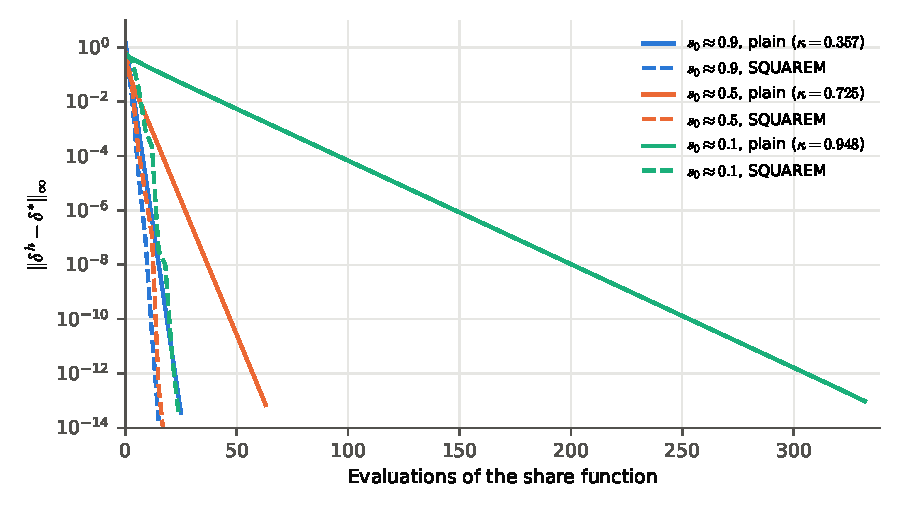
\includegraphics[width=0.92\textwidth]{figures/ch08/fig_contraction.pdf}
  \caption{Convergence of the share inversion in three simulated markets with outside shares near 0.9, 0.5
  and 0.1. Each market has $J = 10$ products, random coefficients with standard deviations
  $(1.0, 1.0, 0.5)$ on the constant, a characteristic and price, and $n_s = 1{,}000$ draws. Solid lines show
  the plain iteration $\delta^{h+1} = \Phi(\delta^h)$. Dashed lines show SQUAREM, the extrapolation method
  described below, on the same map. The
  horizontal axis counts evaluations of the share function. The legend reports the largest row sum $\kappa$
  of the Jacobian of $\Phi$ at the solution. Computed in \texttt{fig\_contraction.py}.}
  \label{fig:08-contraction}
\end{figure}

\subsubsection{Starting values and the multiplicative form}
The logit inversion is the natural first starting value, since it is exact at $\theta_2 = 0$. Inside an
estimation routine the outer optimizer changes $\theta_2$ by small amounts, and the solution at the previous
trial value is a better start. This warm start can cut the number of iterations considerably. Exponentiating
the update gives the equivalent form
\begin{equation*}
  e^{\delta^{h+1}_{jt}} = e^{\delta^h_{jt}}\,\frac{s^{\text{obs}}_{jt}}{s_{jt}(\delta^h_t;\theta_2)},
\end{equation*}
which works with $e^{\delta}$ directly and avoids a logarithm and an exponential per product and iteration.
Each iteration raises $\delta_{jt}$ when the model underpredicts the share of $j$ and lowers it when the model
overpredicts. The individual choice probabilities should be computed with the overflow-safe evaluation of
\cref{sec:08-simulation}.

\subsubsection{The stopping rule}
The iteration stops when successive iterates are close. The next result converts this observable criterion
into a bound on the distance to the solution.

\begin{proposition}[Inner-loop error]\label{prop:08-innererror}
Suppose $\Phi_t$ is a contraction with modulus $\kappa < 1$ on a set that contains the iterates and the
solution $\delta^*_t$. If the iteration stops at the first $H$ with $\Vert \delta^H_t - \delta^{H-1}_t\Vert
\leq \epsilon_{in}$, then
\begin{equation*}
  \Vert \delta^H_t - \delta^*_t \Vert \leq \frac{\kappa}{1 - \kappa}\,\epsilon_{in}.
\end{equation*}
\end{proposition}

\begin{proof}
Since $\delta^*_t = \Phi_t(\delta^*_t)$ and $\delta^H_t = \Phi_t(\delta^{H-1}_t)$,
\begin{align*}
  \Vert \delta^H_t - \delta^*_t\Vert &= \Vert \Phi_t(\delta^{H-1}_t) - \Phi_t(\delta^*_t)\Vert
  \leq \kappa\Vert \delta^{H-1}_t - \delta^*_t\Vert \\
  &\leq \kappa\big(\Vert \delta^{H-1}_t - \delta^{H}_t\Vert + \Vert \delta^H_t - \delta^*_t\Vert\big)
  \leq \kappa\epsilon_{in} + \kappa\Vert \delta^H_t - \delta^*_t\Vert.
\end{align*}
Collecting the terms in $\Vert \delta^H_t - \delta^*_t\Vert$ gives $(1 - \kappa)\Vert \delta^H_t -
\delta^*_t\Vert \leq \kappa\epsilon_{in}$.
\end{proof}

When $\kappa$ is near one, the error can exceed the tolerance by orders of magnitude. In the third market of
\cref{fig:08-contraction} ($\kappa = 0.948$), stopping at a step size of $10^{-4}$ leaves a true error of
$1.0 \times 10^{-3}$, against a bound of $1.7 \times 10^{-3}$. Stopping at $10^{-8}$ leaves $1.0 \times
10^{-7}$. The error is about ten times the tolerance.

The inner error then contaminates the outer problem. Let $e = \tilde\delta - \delta(\theta_2)$ be the
inversion error, stacked over markets. \Cref{sec:08-gmm} shows that the structural error is $\xi(\theta_2) =
\bm{M}\delta(\theta_2)$ for a matrix $\bm{M}$ that does not depend on $\theta_2$ given the weighting matrix.
The computed moments therefore carry the error $\frac{1}{N}\bm{Z}^\T \bm{M} e$. This error varies with
$\theta_2$ in an erratic way, because the number of inner iterations jumps from one trial value to the next.
A finite-difference derivative with step $\Delta$ inherits an error of order $\frac{\Vert e\Vert}{\Delta}$.
With $\Vert e\Vert$ near $10^{-6}$ and $\Delta$ near $10^{-6}$, the error in the computed gradient is of
order one. \citet[Sections~4.2 and~6]{DubeFoxSu2012} show that a loose inner tolerance can keep the outer
optimizer from converging. If the researcher then loosens the outer tolerance, the reported solution may not be a
local minimum. In their synthetic data, no run with inner tolerance $10^{-4}$ and outer tolerance $10^{-6}$
reports convergence (their Table~I). The practical rule is to set the inner
tolerance close to machine precision, for example $10^{-12}$ to $10^{-14}$ in the sup norm, and well below the
outer tolerance. With the warm start this costs little.

\subsubsection{Acceleration}
Two methods speed up the inner loop. The first is SQUAREM, a squared extrapolation method of
\citet{VaradhanRoland2008} designed for slowly converging fixed point iterations.
\citet[Section~2.3]{ReynaertsVaradhanNash2012} apply it to the BLP map. One cycle of the variant we use computes
two plain steps, extrapolates and ends with one more plain step \citep[Table~1]{VaradhanRoland2008}. The step
length $a$ is that of their scheme SqS3, set to $-1$ whenever it exceeds $-1$ (their eqs.~(9) and~(20) and
Section~6):
\begin{gather*}
  r = \Phi(\delta) - \delta, \qquad v = \Phi(\Phi(\delta)) - 2\Phi(\delta) + \delta, \qquad
  a = \min\Big\{-\frac{\Vert r\Vert_2}{\Vert v\Vert_2},\, -1\Big\}, \\
  \delta' = \delta - 2ar + a^2 v, \qquad \delta^{new} = \Phi(\delta').
\end{gather*}
With $a = -1$ the cycle reduces to three plain steps. A more negative $a$ extrapolates along the direction in
which the iterates have been moving. In \cref{fig:08-contraction} SQUAREM reaches an error of $10^{-13}$ after
15, 18 and 24 evaluations of the share function, against 25, 63 and 332 for the plain iteration. Its advantage
grows with the modulus. The second method applies Newton's method to the system $\ln s_t(\delta_t;\theta_2)
= \ln s^{\text{obs}}_t$:
\begin{equation*}
  \delta^{h+1}_t = \delta^h_t - \Big[\frac{\partial \ln s_t(\delta^h_t;\theta_2)}{\partial
  \delta_t^\T}\Big]^{-1}\big(\ln s_t(\delta^h_t;\theta_2) - \ln s^{\text{obs}}_t\big).
\end{equation*}
The Jacobian is available in closed form from the proof of \cref{cor:08-rowsum}, and it is nonsingular by
\cref{rem:08-berry-proof}. Newton's method converges quadratically near the solution but may overshoot far
from it. A common hybrid runs the contraction first and switches to Newton steps once the iterates are close.

\begin{remark}[Dampening in the random coefficients nested logit]\label{rem:08-rcnl}
When random coefficients are combined with a nested logit error with nesting parameter $\rho \in [0,1)$, the
undampened map need not be a contraction. We write the nesting parameter as $\rho$ in this remark, because
$\sigma$ here denotes the standard deviations of the random coefficients.
\citet[pp.~919 and 934--935]{GrigolonVerboven2014} show for the plain nested logit that dampening the step by the
factor $1 - \rho$ restores BLP's sufficient conditions for a contraction. They state that the argument extends to
random coefficients and use the same dampened map in the random coefficients nested logit. The
dampened iteration is $\delta^{h+1} = \delta^h + (1 - \rho)\big(\ln s^{\text{obs}} - \ln s(\delta^h)\big)$. Their
printed equation~(7) attaches the factor $1 - \rho$ to $\ln s(\delta^h)$ alone. \citet[eq.~15 and n.~20]{ConlonGortmaker2020}
point out this typesetting error. In the plain nested logit, $\delta_j
= (1 - \rho)\ln s_j + \rho\ln s_g - \ln s_0$, where $s_g$ is the share of $j$'s nest. Holding the nest and
outside shares fixed, a change in $\ln s_j$ therefore maps into a change of $1 - \rho$ times as much in
$\delta_j$, and the dampened step has this scale. \Cref{ch:mergers} uses this model for merger simulation.
\end{remark}

\section{The GMM estimator}\label{sec:08-gmm}

With the inversion in hand, estimation follows the logic of instrumental variables. This section derives the
estimator, the shortcut that concentrates out the linear parameters, the algorithm, its gradient, the
weighting matrix, and the asymptotic variance with simulation error. It ends with a reformulation as a
constrained optimization problem.

\subsection{Why the error must be the structural error}\label{sec:08-why-xi}

A direct approach would choose the parameters to make predicted shares close to observed shares,
\begin{equation*}
  \min_{\theta}\ \big\Vert s\big(x, p, \delta(x, p, \xi;\theta_1);\theta_2\big) - s^{\text{obs}}\big\Vert,
\end{equation*}
as in equation (7) of \citet{Nevo2000a}. \Citet[pp.~530--531]{Nevo2000a} gives two reasons against it. First,
all parameters enter nonlinearly, and with many brand and time dummies the nonlinear search becomes costly.
Second, and more fundamentally, the approach cannot handle the correlation between prices and $\xi$. The
residual $s^{\text{obs}} - s(\cdot)$ is a nonlinear function of $\xi$. The standard nonlinear simultaneous equations
model allows parameters and variables to enter nonlinearly, but it requires an additively separable error
\citep[p.~531]{Nevo2000a}. The share residual does not have this form. At the true parameters the
predicted share depends on the unknown vector $\xi$. Setting $\xi = 0$ in the prediction leaves a residual
that is a nonlinear function of $\xi$. An orthogonality condition between instruments and $\xi$ then implies no
such condition for the residual.

\citet{Berry1994} proposed to define the econometric error as the structural error $\xi_{jt}$ itself. The
link to economic theory is then direct, and we can reason about which variables are plausibly uncorrelated
with unobserved quality \citep[p.~531]{Nevo2000a}. The cost is the inversion of \cref{sec:08-inversion}.

\subsection{Moment conditions}\label{sec:08-moments}

The identifying assumption of \citet[eq.~4.1]{BerryLevinsohnPakes1995} is a conditional moment restriction.
Let $\mathcal{Z}_t$ denote the exogenous variables of market $t$: the observed characteristics of all products
and the cost shifters. BLP assume
\begin{equation}\label{eq:08-cond-moment}
  \E[\xi_{jt} \mid \mathcal{Z}_t] = 0 \quad\text{and}\quad \E[\omega_{jt} \mid \mathcal{Z}_t] = 0,
\end{equation}
where $\omega_{jt}$ is the cost unobservable of \cref{sec:08-supply}. Prices and quantities are left out of
the conditioning set because the model makes them functions of $\xi$ and $\omega$. The characteristics are
included because the model does not explain how they are chosen \citep[p.~854]{BerryLevinsohnPakes1995}.
\Cref{sec:08-instruments} discusses how plausible this is. In this section we treat demand alone.

A conditional moment restriction implies that $\xi_{jt}$ is uncorrelated with every function of
$\mathcal{Z}_t$. We choose $L$ such functions and collect them in the row vector $z_{jt} \in \R^{1\times L}$,
the \emph{instruments} for observation $(j,t)$. The unconditional moment conditions are
\begin{equation}\label{eq:08-moments}
  \E\big[z_{jt}^\T\,\xi_{jt}(\theta_0)\big] = 0,
\end{equation}
which is equation (8) of \citet{Nevo2000a}. The structural error as a function of the parameters is
\begin{equation}\label{eq:08-xi-theta}
  \xi_{jt}(\theta) = \delta_{jt}(s^{\text{obs}}_t;\theta_2) - x_{jt}\beta + \alpha p_{jt}
\end{equation}
\citep[eq.~13]{Nevo2000a}. The observed shares enter through the inversion. For a trial $\theta_2$, the
inversion finds the mean utilities that rationalize the data. The error is the gap between those mean
utilities and the ones predicted by the linear parameters $(\alpha, \beta)$. When the specification includes
brand and time dummies, they appear on the right-hand side of \eqref{eq:08-xi-theta} and the error becomes the
market-specific deviation $\tilde\xi_{jt}$ of \cref{sec:08-brand-fe}.

We stack the $N = \sum_t J_t$ observations. Let $\delta(\theta_2)$ be the $N$-vector of inverted mean
utilities, $\bm{X}$ the $N \times K_1$ matrix whose rows are $(x_{jt}, p_{jt})$ augmented with any dummies,
and $\theta_1 = (\beta^\T, -\alpha)^\T$ the corresponding coefficient vector. This is the vector of linear
parameters $(\alpha, \beta)$ of \cref{sec:08-linear}, ordered and signed to match the columns of $\bm{X}$. Then
\begin{equation*}
  \xi(\theta) = \delta(\theta_2) - \bm{X}\theta_1.
\end{equation*}
Let $\bm{Z}$ be the $N \times L$ matrix of instruments. The sample moments and the GMM objective are
\begin{equation}\label{eq:08-gmm-obj}
  g_N(\theta) = \frac{1}{N}\bm{Z}^\T\xi(\theta), \qquad
  Q_N(\theta) = g_N(\theta)^\T W g_N(\theta) = \frac{1}{N^2}\,\xi(\theta)^\T\bm{Z}W\bm{Z}^\T\xi(\theta),
\end{equation}
for a positive definite $L \times L$ weighting matrix $W$. This is equation (9) of \citet{Nevo2000a} and
equation (6) of \citet{Nevo2001}, who write $W$ as the inverse of an estimate of $\E[\bm Z^\T\xi\xi^\T\bm Z]$.
The GMM estimator is $\hat\theta = \argmin_\theta Q_N(\theta)$. The order condition
requires $L \geq K_1 + K_2$, where $K_2 = \dim\theta_2$. The rank condition requires that
$\E[z_{jt}^\T\frac{\partial \xi_{jt}(\theta_0)}{\partial \theta^\T}]$ have full column rank.
\Cref{app:econometrics} reviews the general theory.

\subsection{Concentrating out the linear parameters}\label{sec:08-concentrate}

The objective \eqref{eq:08-gmm-obj} is quadratic in $\theta_1$ for fixed $\theta_2$. The linear parameters
can therefore be solved in closed form \citep[p.~868]{BerryLevinsohnPakes1995}.

\begin{proposition}[Concentrating out $\theta_1$]\label{prop:08-concentrate}
Suppose $\bm{X}^\T\bm{Z}W\bm{Z}^\T\bm{X}$ is nonsingular. For each $\theta_2$, the value of $\theta_1$ that
minimizes $Q_N(\theta_1, \theta_2)$ is
\begin{equation}\label{eq:08-theta1hat}
  \hat\theta_1(\theta_2) = \big(\bm{X}^\T\bm{Z}W\bm{Z}^\T\bm{X}\big)^{-1}\bm{X}^\T\bm{Z}W\bm{Z}^\T\delta(\theta_2).
\end{equation}
The implied structural error is $\xi(\theta_2) = \bm{M}\delta(\theta_2)$ with $\bm{M} = I_N -
\bm{X}(\bm{X}^\T\bm{Z}W\bm{Z}^\T\bm{X})^{-1}\bm{X}^\T\bm{Z}W\bm{Z}^\T$. The GMM estimator of $\theta_2$
minimizes the profiled objective
\begin{equation}\label{eq:08-profiled}
  Q^c_N(\theta_2) = \frac{1}{N^2}\,\delta(\theta_2)^\T\bm{M}^\T\bm{Z}W\bm{Z}^\T\bm{M}\,\delta(\theta_2),
\end{equation}
and $\hat\theta_1 = \hat\theta_1(\hat\theta_2)$.
\end{proposition}

\begin{proof}
Fix $\theta_2$ and write $\delta = \delta(\theta_2)$. The objective is
\begin{equation*}
  Q_N = \frac{1}{N^2}(\delta - \bm{X}\theta_1)^\T\bm{Z}W\bm{Z}^\T(\delta - \bm{X}\theta_1).
\end{equation*}
Its gradient with respect to $\theta_1$ is
\begin{equation*}
  \frac{\partial Q_N}{\partial \theta_1} = -\frac{2}{N^2}\bm{X}^\T\bm{Z}W\bm{Z}^\T(\delta - \bm{X}\theta_1).
\end{equation*}
Setting it to zero gives the normal equations $\bm{X}^\T\bm{Z}W\bm{Z}^\T\bm{X}\,\theta_1 =
\bm{X}^\T\bm{Z}W\bm{Z}^\T\delta$, whose solution is \eqref{eq:08-theta1hat}. The Hessian
$\frac{2}{N^2}\bm{X}^\T\bm{Z}W\bm{Z}^\T\bm{X}$ is positive definite, so this is the unique minimum.
Substituting, $\delta - \bm{X}\hat\theta_1(\theta_2) = \bm{M}\delta$, and the objective at the minimum is
\eqref{eq:08-profiled}. Finally, $\min_{\theta_1,\theta_2}Q_N = \min_{\theta_2}\min_{\theta_1}Q_N =
\min_{\theta_2}Q^c_N(\theta_2)$.
\end{proof}

The matrix $\bm{M}$ depends on the data and on $W$ only. It can be computed once for each weighting matrix,
and each objective evaluation then requires one matrix-vector product. The nonlinear search runs over
$\theta_2$ alone, which typically has a handful of elements. The number of random coefficients therefore drives the
cost of estimation. The mean utility can include many characteristics, and even brand dummies, at little cost
(\cref{sec:08-model}).

\begin{corollary}[Logit and nested logit as 2SLS]\label{cor:08-2sls}
In the logit model $\theta_2$ is empty and $\delta_{jt} = \ln s^{\text{obs}}_{jt} - \ln s^{\text{obs}}_{0t}$. With $W =
(\frac{1}{N}\bm{Z}^\T\bm{Z})^{-1}$, the estimator \eqref{eq:08-theta1hat} is two-stage least squares of
$\ln s_{jt} - \ln s_{0t}$ on $\bm{X}$ with instruments $\bm{Z}$. In the nested logit model the same holds
after adding $\ln s_{j|g,t}$ to $\bm{X}$ as a second endogenous regressor with coefficient $\sigma$.
\end{corollary}

\begin{proof}
Write $P_Z = \bm{Z}(\bm{Z}^\T\bm{Z})^{-1}\bm{Z}^\T$. The scalar $\frac{1}{N}$ in $W$ cancels from
\eqref{eq:08-theta1hat}, which becomes $(\bm{X}^\T P_Z\bm{X})^{-1}\bm{X}^\T P_Z\delta$, the 2SLS formula. In
the nested logit model $\ln s_{jt} - \ln s_{0t} = x_{jt}\beta - \alpha p_{jt} + \sigma\ln s_{j|g,t} +
\xi_{jt}$, which is linear in $(\beta, \alpha, \sigma)$.
\end{proof}

\Citet[p.~533 and n.~22]{Nevo2000a} and \citet[p.~319]{Nevo2001} make the same point. The weighting matrix
$(\bm{Z}^\T\bm{Z})^{-1}$ is efficient when the errors are homoskedastic.

\subsection{The nested fixed point algorithm}\label{sec:08-nfxp}

The estimator nests the inversion (a fixed point problem) inside the minimization. We call the procedure the
\emph{nested fixed point} (NFXP) algorithm. \citet[p.~863]{BerryLevinsohnPakes1995} describe four steps for
each evaluation of the moments. They estimate the market shares by simulation and solve for the demand
unobservables. They then compute the cost unobservables as price minus the markup, and they interact both
unobservables with the instruments. In our notation the algorithm reads as follows.

\begin{enumerate}[label=\arabic*.,leftmargin=2em]
  \item Before the search, draw $(D_i, \nu_i)$, $i = 1, \dots, n_s$, for each market and hold the draws fixed
  for the whole estimation. Choose the first-step weighting matrix $W = (\frac{1}{N}\bm{Z}^\T\bm{Z})^{-1}$ and
  compute $\bm{M}$.
  \item The outer optimizer proposes a value $\theta_2^{(k)}$. Compute $\mu_{ijt} = \tilde x_{jt}(\Pi D_i +
  \Sigma\nu_i)$ for all draws, products and markets.
  \item In each market, iterate $\delta^{h+1}_t = \Phi_t(\delta^h_t)$ from the last solution until $\Vert
  \delta^{h+1}_t - \delta^h_t\Vert_\infty < \epsilon_{in}$, using the simulated share $s^{n_s}_t$ of
  \cref{sec:08-simulation}.
  \item Compute $\hat\theta_1(\theta_2^{(k)})$ by \eqref{eq:08-theta1hat} and $\xi(\theta_2^{(k)}) =
  \bm{M}\delta(\theta_2^{(k)})$. With a supply side, also compute the markups and the cost unobservable
  $\omega$ (\cref{sec:08-supply}).
  \item Evaluate $Q^c_N(\theta_2^{(k)})$ and its gradient (\cref{prop:08-gradient}). Return them to the
  optimizer, which either stops or returns to step 2.
  \item After convergence, compute the second-step weighting matrix from the first-step residuals
  (\cref{sec:08-weighting}) and repeat steps 2 to 5.
\end{enumerate}

\Cref{fig:08-nfxp} displays the algorithm. Two remarks concern the outer search. \citet[p.~868]%
{BerryLevinsohnPakes1995} use the Nelder-Mead simplex method, which needs no derivatives. \citet[p.~319]%
{Nevo2001} uses a quasi-Newton method with an analytic gradient and reports that it ``was found to work much
faster.'' Holding the draws fixed is essential for the outer search. Fresh draws at each evaluation would make
the objective a random function of $\theta_2$, and no optimizer would converge \citep{PakesPollard1989}.

\begin{figure}[htbp]
\centering
\begin{tikzpicture}[
  node distance=5mm,
  box/.style={draw, rounded corners=2pt, align=center, font=\small, text width=7.4cm, inner sep=4pt},
  dec/.style={draw, diamond, aspect=3.2, align=center, font=\small, inner sep=0.5pt},
  note/.style={draw, dashed, rounded corners=2pt, align=left, font=\footnotesize, text width=3.3cm,
    inner sep=3pt},
  arr/.style={-{Stealth[length=2.2mm]}, thick}]
\node[box] (draws) {Draw $(D_i, \nu_i)$, $i = 1, \dots, n_s$, in each market once and hold them fixed.
  Set $W = (\frac{1}{N}\bm{Z}^\T\bm{Z})^{-1}$};
\node[box, below=of draws] (outer) {Outer step: the optimizer proposes $\theta_2^{(k)}$};
\node[box, below=of outer] (mu) {Compute $\mu_{ijt} = \tilde x_{jt}(\Pi D_i + \Sigma\nu_i)$\\ for all $i$, $j$, $t$};
\node[box, below=of mu] (inner) {Inner step in each market:\\ $\delta^{h+1}_t = \delta^{h}_t + \ln s^{\text{obs}}_t
  - \ln s^{n_s}_t(\delta^h_t;\theta_2^{(k)})$};
\node[dec, below=of inner] (tol) {$\Vert\delta^{h+1}_t - \delta^{h}_t\Vert_\infty < \epsilon_{in}$?};
\node[box, below=of tol] (lin) {Concentrate out $\hat\theta_1(\theta_2^{(k)})$\\ and set
  $\xi(\theta_2^{(k)}) = \bm{M}\delta(\theta_2^{(k)})$.\\ With a supply side, also $\omega(\theta^{(k)})$};
\node[box, below=of lin] (obj) {Objective $Q^c_N(\theta_2^{(k)})$ and gradient $\nabla Q^c_N(\theta_2^{(k)})$};
\node[dec, below=of obj] (conv) {Outer stopping rule met?};
\node[box, below=of conv] (done) {Report $\hat\theta_2$ and $\hat\theta_1(\hat\theta_2)$.
  Update $W$ and repeat (second step)};
\draw[arr] (draws) -- (outer);
\draw[arr] (outer) -- (mu);
\draw[arr] (mu) -- (inner);
\draw[arr] (inner) -- (tol);
\draw[arr] (tol) -- node[right, font=\footnotesize] {yes} (lin);
\draw[arr] (tol.east) -| node[above, font=\footnotesize, pos=0.25] {no} ([xshift=6mm]inner.east)
  -- (inner.east);
\draw[arr] (lin) -- (obj);
\draw[arr] (obj) -- (conv);
\draw[arr] (conv) -- node[right, font=\footnotesize] {yes} (done);
\draw[arr] (conv.west) -| node[above, font=\footnotesize, pos=0.25] {no} ([xshift=-6mm]outer.west)
  -- (outer.west);
\node[note, right=1.4cm of inner] {Warm start from the last $\delta_t$. Tolerance near machine precision.
  SQUAREM or Newton steps speed it up};
\node[note, right=1.4cm of obj] {Gradient by \cref{prop:08-gradient}. Optimizer: Nelder-Mead or
  quasi-Newton};
\end{tikzpicture}
\caption{The nested fixed point algorithm. The outer loop searches over the nonlinear parameters
$\theta_2$. For each trial value the inner loop inverts the share equations market by market, the linear
parameters are concentrated out, and the profiled GMM objective is evaluated.}
\label{fig:08-nfxp}
\end{figure}

\subsection{The gradient}\label{sec:08-gradient}

Quasi-Newton methods need the gradient of $Q^c_N$. Because $\delta(\theta_2)$ is defined implicitly by the
share equations, its derivative comes from the implicit function theorem (\cref{app:math}).

\begin{proposition}[Gradient of the profiled objective]\label{prop:08-gradient}
For each market, $\delta_t(\theta_2)$ is continuously differentiable and
\begin{equation}\label{eq:08-ift}
  \frac{\partial \delta_t}{\partial \theta_2^\T} = -\Big[\frac{\partial s_t}{\partial
  \delta_t^\T}\Big]^{-1}\frac{\partial s_t}{\partial \theta_2^\T}.
\end{equation}
In the random coefficients logit model with diagonal $\Sigma = \diag(\sigma_1, \dots, \sigma_{K+1})$ and
demographic coefficients $\pi_{kd}$, the derivatives on the right are
\begin{align}
  \frac{\partial s_{jt}}{\partial \delta_{kt}} &= \int s_{ijt}\big(\indic\{j = k\} - s_{ikt}\big)\, \dd F,
  \notag\\
  \frac{\partial s_{jt}}{\partial \sigma_k} &= \int s_{ijt}\,\nu_{ik}\Big(\tilde x_{jtk} - \sum_{m \in
  \mathcal{J}_t}s_{imt}\tilde x_{mtk}\Big)\, \dd F, \label{eq:08-dsdsigma}\\
  \frac{\partial s_{jt}}{\partial \pi_{kd}} &= \int s_{ijt}\,D_{id}\Big(\tilde x_{jtk} - \sum_{m \in
  \mathcal{J}_t}s_{imt}\tilde x_{mtk}\Big)\, \dd F. \notag
\end{align}
The gradient of the profiled objective is
\begin{equation}\label{eq:08-grad}
  \nabla Q^c_N(\theta_2) = \frac{2}{N^2}\Big(\frac{\partial \delta}{\partial \theta_2^\T}\Big)^\T
  \bm{Z}W\bm{Z}^\T\xi(\theta_2).
\end{equation}
\end{proposition}

\begin{proof}
The inverted mean utilities satisfy the identity $s_t(\delta_t(\theta_2);\theta_2) = s^{\text{obs}}_t$ for all
$\theta_2$. Differentiating with respect to $\theta_2^\T$ gives
\begin{equation*}
  \frac{\partial s_t}{\partial \delta_t^\T}\,\frac{\partial \delta_t}{\partial \theta_2^\T} +
  \frac{\partial s_t}{\partial \theta_2^\T} = 0.
\end{equation*}
The Jacobian $\frac{\partial s_t}{\partial \delta_t^\T}$ is nonsingular by \cref{rem:08-berry-proof}, so the
implicit function theorem applies and yields \eqref{eq:08-ift}. The derivative with respect to $\delta$ was
computed in the proof of \cref{cor:08-rowsum}. For $\sigma_k$, note that $\mu_{ijt} = \sum_k \tilde
x_{jtk}(\sigma_k\nu_{ik} + \sum_d \pi_{kd}D_{id})$, so $\frac{\partial \mu_{ijt}}{\partial \sigma_k} = \tilde
x_{jtk}\nu_{ik}$. From $\ln s_{ijt} = \delta_{jt} + \mu_{ijt} - \ln(1 + \sum_m e^{\delta_{mt} + \mu_{imt}})$,
\begin{equation*}
  \frac{\partial \ln s_{ijt}}{\partial \sigma_k} = \tilde x_{jtk}\nu_{ik} - \sum_m s_{imt}\tilde
  x_{mtk}\nu_{ik},
\end{equation*}
and multiplying by $s_{ijt}$ and integrating gives \eqref{eq:08-dsdsigma}. The derivative with respect to
$\pi_{kd}$ replaces $\nu_{ik}$ by $D_{id}$. For the gradient, write $Q_N(\theta_1, \theta_2)$ as in
\eqref{eq:08-gmm-obj}, so $Q^c_N(\theta_2) = Q_N(\hat\theta_1(\theta_2), \theta_2)$. By the chain rule,
\begin{equation*}
  \nabla Q^c_N = \frac{\partial Q_N}{\partial \theta_2} + \Big(\frac{\partial \hat\theta_1}{\partial
  \theta_2^\T}\Big)^\T\frac{\partial Q_N}{\partial \theta_1}.
\end{equation*}
The second term vanishes because $\frac{\partial Q_N}{\partial \theta_1} = 0$ at $\hat\theta_1(\theta_2)$.
This is the envelope theorem. Holding $\theta_1$ fixed, $\frac{\partial \xi}{\partial \theta_2^\T} =
\frac{\partial \delta}{\partial \theta_2^\T}$, which gives \eqref{eq:08-grad}.
\end{proof}

With simulation, every integral in the proposition is replaced by the average over the $n_s$ fixed draws.
The gradient then costs about as much as one more share evaluation plus the solution of a $J_t \times J_t$
linear system in each market. The matrix $\frac{\partial \delta}{\partial \theta_2^\T}$ also reappears in the
asymptotic variance below and in the optimal instruments of \cref{sec:08-optiv}.

\subsection{Weighting, efficiency and clustering}\label{sec:08-weighting}

The efficient weighting matrix is the inverse of the variance of the moments. With independent observations
the second-step matrix is
\begin{equation*}
  W_2 = \Big[\frac{1}{N}\sum_t\sum_{j \in \mathcal{J}_t} z_{jt}^\T\,\hat\xi_{jt}^2\, z_{jt}\Big]^{-1},
\end{equation*}
where $\hat\xi_{jt}$ are the residuals at the first-step estimate. \citet[p.~319]{Nevo2001} follows this
two-step procedure. He also iterated further and found that ``the estimated parameters changed only slightly
beyond the second iteration.''

Errors are often correlated within groups of observations. \citet[pp.~862--863]{BerryLevinsohnPakes1995}
follow car models over the years they are sold, and the unobservables of one model are more alike across years
than across models. They sum the moments of each model over its years,
\begin{equation*}
  g_m(\theta) = \sum_t \big[f_{mt}(\mathcal{Z})^\T \otimes I_2\big]
  \begin{pmatrix}\xi_{mt}(\theta)\\ \omega_{mt}(\theta)\end{pmatrix},
\end{equation*}
where $f_{mt}(\mathcal{Z})$ is the vector of instrument functions for model $m$ in year $t$ and $\otimes$ is
the Kronecker product. They then minimize a quadratic form in the average of $g_m$ over models. The
resulting standard errors allow arbitrary correlation across years for a given model and arbitrary
heteroskedasticity across models. The corresponding efficient weighting matrix is the inverse of $\frac{1}{M}
\sum_m g_m(\hat\theta)g_m(\hat\theta)^\T$, with $M$ the number of models. The same construction applies with
cities, markets or brands as clusters (\cref{app:econometrics}).

With the efficient weighting matrix, $N\,Q_N(\hat\theta)$ is the \emph{Hansen J statistic}. Under correct
specification it converges in distribution to a $\chi^2$ with $L - K_1 - K_2$ degrees of freedom. A rejection
signals that some instruments are invalid or that the model is misspecified. With tens of thousands of
observations the test rejects almost any model, as \citet[p.~325, n.~23]{Nevo2001} notes.

\subsection{Asymptotic distribution and simulation error}\label{sec:08-asymptotics}

The estimator departs from textbook GMM in two ways. The moments are computed from sampled shares, and the
share integral is simulated. \citet[Section 5]{BerryLevinsohnPakes1995} account for both. Their setting is a
single cross section of $J$ products, with asymptotics as $J$ grows. Let $s^0$ be the population shares,
$s^n$ the shares observed in a sample of $n$ consumers, $P_0$ the distribution of consumer attributes, and
$P_{n_s}$ the empirical distribution of $n_s$ simulation draws. BLP standardize the two unobservables by a
$2 \times 2$ matrix $T(z_j)$ with $T(z_j)^\T T(z_j) = \Upsilon(z_j)^{-1}$, where $\Upsilon(z_j) =
\E[(\xi_j, \omega_j)^\T(\xi_j, \omega_j) \mid z_j]$ (their eqs.~5.1--5.2). BLP write $\Omega$ for this covariance matrix. We write $\Upsilon$ because $\Omega$ is the ownership matrix in this book. They interact the standardized
errors with an $L \times 2$ instrument matrix $H_j(\mathcal Z)$ and form
\begin{equation*}
  G_J(\theta; s, P) = \frac{1}{J}\sum_{j=1}^{J}H_j(\mathcal{Z})\,T(z_j)\begin{pmatrix}\xi_j(\theta, s,
  P)\\ \omega_j(\theta, s, P)\end{pmatrix}
\end{equation*}
(eq.~5.4). The estimator minimizes $\Vert G_J(\theta; s^n, P_{n_s})\Vert$ with $\Vert y\Vert = y^\T y$
(eq.~5.5).

The computed moments differ from the ideal ones $G_J(\theta_0; s^0, P_0)$ in two ways. Adding and subtracting
gives the decomposition
\begin{multline*}
  G_J(\theta_0; s^n, P_{n_s}) = \underbrace{G_J(\theta_0; s^0, P_0)}_{\text{product draws}}
  + \underbrace{\big[G_J(\theta_0; s^n, P_0) - G_J(\theta_0; s^0, P_0)\big]}_{\text{consumer sampling}}\\
  + \underbrace{\big[G_J(\theta_0; s^n, P_{n_s}) - G_J(\theta_0; s^n, P_0)\big]}_{\text{simulation}}.
\end{multline*}
The three terms come from three independent random processes: the draws of the product characteristics
$(x, w, \xi, \omega)$, the sampling of consumers, and the simulation draws. Their variances, scaled by $J$,
converge to
\begin{align*}
  V_1 &= \lim_{J\to\infty}\E_{\mathcal Z}\Big[H_j T(z_j)\begin{pmatrix}\xi_j\\ \omega_j\end{pmatrix}
  \begin{pmatrix}\xi_j\\ \omega_j\end{pmatrix}^\T T(z_j)^\T H_j^\T\Big],\\
  V_2 &= \lim_{J\to\infty}\frac{J}{n}\,\E\Big(n\big[G_J(\theta_0; s^0, P_0) - G_J(\theta_0; s^n,
  P_0)\big]\big[\cdot\big]^\T\Big),\\
  V_3 &= \lim_{J\to\infty}\frac{J}{n_s}\,\E\Big(n_s\big[G_J(\theta_0; s^n, P_{n_s}) - G_J(\theta_0; s^n,
  P_0)\big]\big[\cdot\big]^\T \,\Big|\, s^n\Big),
\end{align*}
where $[\cdot]$ repeats the preceding bracket. The usual GMM linearization then applies. The first-order
condition $\hat G^\T G_J(\hat\theta) = 0$, with $\hat G$ the Jacobian of the moments, and a mean value expansion
$G_J(\hat\theta) \approx G_J(\theta_0) + G(\hat\theta - \theta_0)$ give $\sqrt{J}(\hat\theta - \theta_0)
\approx -(G^\T G)^{-1}G^\T\sqrt{J}\,G_J(\theta_0)$. Hence the asymptotic variance is
\begin{equation}\label{eq:08-blp-avar}
  (G^\T G)^{-1}G^\T(V_1 + V_2 + V_3)\,G\,(G^\T G)^{-1}, \qquad G = \lim_{J\to\infty}\frac{\partial
  \E[G_J(\theta, s^0, P_0)]}{\partial \theta^\T}\Big|_{\theta = \theta_0},
\end{equation}
which is equation (5.6) of \citet{BerryLevinsohnPakes1995}, who write $\Gamma$ for $G$. With a general
weighting matrix the formula becomes $(G^\T WG)^{-1}G^\T W(V_1 + V_2 + V_3)WG(G^\T WG)^{-1}$.

The scale factors explain which terms matter. $V_2$ carries the factor $\frac{J}{n}$, and BLP note that $n$,
the number of U.S. households, ``is on the order of 100 million,'' so $V_2$ is negligible
\citep[p.~859]{BerryLevinsohnPakes1995}. $V_3$ carries the factor $\frac{J}{n_s}$, and with a feasible number
of draws it is not negligible. The limit theory requires $n$ and $n_s$ to grow ``on the order of $J^3$''
(p.~859). The ``in process'' paper that BLP cite for these results was published as
\citet{BerryLintonPakes2004}. Its theorems need the number of draws to grow only at rate $J^2$ in
logit-style models, a weaker condition than the rate BLP quote (\cref{sec:08-pcm}). BLP estimate $V_1$ by its sample analog at $\hat\theta$. They estimate $V_3$ by
drawing new sets of simulation draws, recomputing the moments at $\hat\theta$ for each set, and taking the
empirical variance. The correction ``increases our reported standard errors \dots by about 5--20\% (with the
exception of one parameter, whose reported standard error doubles)'' (p.~859).

The sampling scheme behind $V_1$ deserves a word. BLP do not assume that products are independent draws. They
assume that the vectors $y_j = (\xi_j, \omega_j, z_j)$ are \emph{exchangeable}: their joint density is
unchanged by any permutation of the product labels \citep[p.~856, n.~14]{BerryLevinsohnPakes1995}. This
allows characteristics chosen by firms to be related across products and allows common shocks to many
products.

In data with many markets and a fixed set of products, as in \citet{Nevo2001}, the asymptotics run over
markets instead. The moments are averages of independent market-level terms, and the usual cluster-robust
GMM formulas apply. \citet[p.~319]{Nevo2001} corrects for simulation error by accounting for the fact that
the draws are common to all observations in a market. One caveat carries over from \cref{sec:08-simulation}.
The log of a simulated share is biased (\cref{prop:08-simbias}), so the inverted $\delta$ carries a bias of
order $\frac{1}{n_s}$ that does not average out across markets. Consistency therefore requires $n_s$ to grow
with the sample, and in practice $n_s$ should be large enough that the bias is small relative to the standard
errors.

Two practical points complete the picture. First, the standard errors must be computed for the full
parameter vector $\theta = (\theta_1, \theta_2)$. The moment Jacobian is
\begin{equation*}
  G = \frac{1}{N}\bm{Z}^\T\Big[-\bm{X},\ \frac{\partial \delta}{\partial \theta_2^\T}\Big],
\end{equation*}
with the second block from \cref{prop:08-gradient}. Treating the second-stage regression
\eqref{eq:08-theta1hat} as ordinary 2SLS with $\delta$ as data ignores the estimation of $\theta_2$ and
understates the uncertainty in $\hat\theta_1$. Second, objects such as elasticities, markups and welfare are
nonlinear functions $\varphi(\theta)$. Their uncertainty can be computed by the delta method,
$\widehat{\Var}(\varphi(\hat\theta)) = \nabla\varphi^\T\widehat{\Var}(\hat\theta)\nabla\varphi$, or by a
parametric bootstrap. The bootstrap draws $\theta^{(r)}$ from the estimated asymptotic distribution of
$\hat\theta$, computes $\varphi(\theta^{(r)})$ for each draw, and reads off percentiles.
\citet[pp.~319, 333]{Nevo2001} uses the bootstrap, with 1,500 draws for the margins of his Table VIII
(\cref{sec:08-nevo01}).

\subsection{MPEC: estimation as constrained optimization}\label{sec:08-mpec}

\citet{SuJudd2012} propose to estimate structural models by \emph{mathematical programming with equilibrium
constraints} (MPEC), and \citet{DubeFoxSu2012} apply the idea to BLP. Instead of solving the share equations
for every trial value of $\theta_2$, MPEC treats the mean utilities as additional unknowns and imposes the
share equations as constraints:
\begin{equation}\label{eq:08-mpec}
  \min_{\theta_1, \theta_2, \delta, \eta}\ \eta^\T W\eta \quad\text{subject to}\quad
  s_t(\delta_t;\theta_2) = s^{\text{obs}}_t \ \ (t = 1, \dots, T), \qquad
  \eta = \frac{1}{N}\bm{Z}^\T(\delta - \bm{X}\theta_1).
\end{equation}
The auxiliary vector $\eta \in \R^L$ holds the sample moments.

\begin{proposition}[Equivalence of MPEC and NFXP]\label{prop:08-mpec}
Suppose the conditions of \cref{thm:08-berry94} hold for every $\theta_2$ in the parameter space. Then
$(\hat\theta_1, \hat\theta_2)$ minimizes the GMM objective \eqref{eq:08-gmm-obj} if and only if there exist
$\hat\delta$ and $\hat\eta$ such that $(\hat\theta_1, \hat\theta_2, \hat\delta, \hat\eta)$ solves
\eqref{eq:08-mpec}. In that case $\hat\delta = \delta(\hat\theta_2)$ and $\hat\eta = g_N(\hat\theta)$.
\end{proposition}

\begin{proof}
By \cref{thm:08-berry94}, for each $\theta_2$ the share constraints have exactly one solution,
$\delta(\theta_2)$. The second constraint then determines $\eta$. The feasible set of \eqref{eq:08-mpec} is
therefore
\begin{equation*}
  \Big\{\big(\theta_1, \theta_2, \delta(\theta_2), \frac{1}{N}\bm{Z}^\T(\delta(\theta_2) -
  \bm{X}\theta_1)\big): (\theta_1, \theta_2) \text{ in the parameter space}\Big\}.
\end{equation*}
On this set the objective equals $g_N(\theta)^\T Wg_N(\theta) = Q_N(\theta)$. Minimizing over the feasible set
is the same as minimizing $Q_N$ over $\theta$, and the minimizers correspond one to one. The map
$\theta_2 \mapsto \delta(\theta_2)$ is continuous by \cref{prop:08-gradient}, so local minimizers also
correspond.
\end{proof}

The two formulations have the same solutions and different computational properties. MPEC has no inner loop,
so there is no inner tolerance and no propagation of inversion error into the objective. The share
constraints need hold only at the solution, so the solver does not spend effort on precise inversions at trial
values far from the optimum. The constraint Jacobian is sparse, because $s_t$ depends only on $\delta_t$ and
$\theta_2$. Derivatives can be supplied by automatic differentiation. Against this, the problem has $K_1 +
K_2 + N + L$ unknowns, $N$ nonlinear share constraints and $L$ linear moment constraints. It requires a large-scale constrained solver and
careful scaling, and the solver may stop at an infeasible point. \citet[Section~7]{DubeFoxSu2012} find MPEC
faster than NFXP when the contraction is slow. By \cref{cor:08-rowsum}, this happens when outside shares are
small. With an outside share of 0.35 in their experiments, MPEC is about 24 times faster (their Table~III).
\citet[Sections~3 and~5]{ConlonGortmaker2020} instead use the nested fixed point. They prefer an inner tolerance
between $10^{-14}$ and $10^{-12}$. They find SQUAREM the fastest and most reliable way to accelerate the
contraction.
The choice between the two is a matter of implementation. The statistical properties of the estimator are the same.

Other estimators trade exactness for speed. \citet[Section~5]{LeeSeo2015} linearize the log share function around
the current mean utilities and invert this approximation analytically at each trial value. After each minimization
they update the point of approximation by one Newton step. The share equations therefore hold exactly only at the
optimum.
\citet[Sections~2 and~3]{SalanieWolak2019} expand the inverse share function to second order around zero random
coefficients. The resulting approximate model is linear in the mean coefficients and in the variances and
covariances of the random coefficients. Two-stage least squares therefore estimates it. These estimates can serve as
starting values for the exact estimator.
\Cref{prop:08-smallsigma} below derives the leading term of such an expansion.

\section{Instruments and identification}\label{sec:08-instruments}

The estimator of \cref{sec:08-gmm} is only as good as its instruments. This section first explains why prices
need instruments, how many instruments are needed and which roles they play. It then derives the efficient
instruments and reviews the instrument families used in practice. It closes with brand fixed effects and with
nonparametric identification.

\subsection{Price endogeneity}\label{sec:08-endogeneity}

Firms observe $\xi_{jt}$ when they set prices. In a Nash-Bertrand equilibrium the price is marginal cost
plus a markup (\cref{ch:diffprod}), and the markup depends on demand, hence on $\xi_t$. \citet[eq.~8]%
{Nevo2001} writes
\begin{equation*}
  p_{jt} = mc_{jt} + f(\xi_{jt}, \dots) = (mc_j + f_j) + \big(mc_{jt} - mc_j + f_{jt} - f_j\big),
\end{equation*}
where $mc_j$ and $f_j$ are brand means and the second bracket is the deviation of the market from them. With
brand dummies the brand means are absorbed, but the market-specific deviation of the markup still moves with
the market-specific deviation of $\xi$ \citep[p.~320]{Nevo2001}.

A single-product logit firm makes the sign transparent. Its first-order condition gives the markup $m_j =
p_j - mc_j = \frac{1}{\alpha(1 - s_j)}$ (\cref{ch:logit}). Hold rivals' prices fixed and define
\begin{equation*}
  G(m_j, \xi_j) = m_j - \frac{1}{\alpha\big(1 - s_j(m_j, \xi_j)\big)},
\end{equation*}
where $s_j$ is the logit share at price $mc_j + m_j$. The optimal markup solves $G(m_j, \xi_j) = 0$. The logit
derivatives are $\frac{\partial s_j}{\partial m_j} = -\alpha s_j(1 - s_j)$ and $\frac{\partial s_j}{\partial
\xi_j} = s_j(1 - s_j)$. By the chain rule,
\begin{align*}
  \frac{\partial}{\partial m_j}\,\frac{1}{\alpha(1 - s_j)} &= \frac{1}{\alpha(1 - s_j)^2}\,\frac{\partial
  s_j}{\partial m_j} = -\frac{s_j}{1 - s_j},\\
  \frac{\partial}{\partial \xi_j}\,\frac{1}{\alpha(1 - s_j)} &= \frac{1}{\alpha(1 - s_j)^2}\,\frac{\partial
  s_j}{\partial \xi_j} = \frac{s_j}{\alpha(1 - s_j)}.
\end{align*}
Hence
\begin{equation*}
  \frac{\partial G}{\partial m_j} = 1 + \frac{s_j}{1 - s_j} = \frac{1}{1 - s_j}, \qquad
  \frac{\partial G}{\partial \xi_j} = -\frac{s_j}{\alpha(1 - s_j)}.
\end{equation*}
The implicit function theorem then gives the response of the best-response markup to unobserved quality,
\begin{equation*}
  \frac{\partial m_j}{\partial \xi_j} = -\frac{\partial G}{\partial \xi_j}\Big(\frac{\partial G}{\partial
  m_j}\Big)^{-1} = \frac{s_j}{\alpha(1 - s_j)}\,(1 - s_j) = \frac{s_j}{\alpha} > 0.
\end{equation*}
A better unobserved product sells more and carries a higher markup, so $\Cov(p_{jt}, \xi_{jt}) > 0$.

Consider the logit estimating equation $\ln s_{jt} - \ln s_{0t} = x_{jt}\beta - \alpha p_{jt} + \xi_{jt}$
and let $\tilde p_{jt}$ be the residual from projecting $p_{jt}$ on $x_{jt}$. By the Frisch-Waugh theorem the
OLS coefficient on price satisfies
\begin{equation*}
  \plim\, \widehat{(-\alpha)}_{OLS} = -\alpha + \frac{\Cov(\tilde p_{jt}, \xi_{jt})}{\Var(\tilde p_{jt})}
  > -\alpha,
\end{equation*}
when $x_{jt}$ is uncorrelated with $\xi_{jt}$. The estimated price coefficient is biased toward zero, and
demand looks too inelastic. Random coefficients do not remove the problem, since $\xi_{jt}$ enters
$\delta_{jt}$ in the same way.

The evidence matches the theory. In the automobile data of \citet[Table III]{BerryLevinsohnPakes1995}, the
OLS logit price coefficient is $-0.089$ (0.004). It implies that 1,494 of the 2,217 models have inelastic
demand, which is inconsistent with profit maximization. With instruments the coefficient becomes $-0.216$
(0.123), and only 22 models have inelastic demand (pp.~873--874). In the cereal data of \citet[Table V]%
{Nevo2001}, the OLS logit coefficient with brand dummies is $-7.26$ (0.16). The same specification
instrumented with prices in other cities gives $-17.57$ (0.50) (columns ii and v). \Cref{sec:08-blp95,sec:08-nevo01} present these tables in
full.

\subsection{How many instruments, and what they must do}\label{sec:08-iv-roles}

The order condition of \cref{sec:08-moments} counts the instruments. The exogenous characteristics in
$x_{jt}$ serve as their own instruments. The remaining instruments must be at least as many as the
endogenous variables in the mean utility (usually price alone) plus the number of nonlinear parameters. A
model with one random coefficient per characteristic and on price needs $K + 2$ excluded instruments,
where $K$ is the number of characteristics: one for price and $K + 1$ for $\Sigma$.

The instruments play two distinct roles. Some must shift prices, as in any demand system. Others must shift
what \citet[Section 7]{BerryHaile2014} call ``quantities,'' the market shares that enter the inverse demand
function. \citet[p.~1136, n.~2]{BerryHaile2024} note that instruments for quantities are what the applied
literature informally calls instruments for the ``nonlinear parameters.'' The next result shows concretely why
the nonlinear parameters need their own source of variation.

\begin{proposition}[Small-$\sigma$ expansion of the inverse]\label{prop:08-smallsigma}
Suppose there is a single random coefficient, $\mu_{ijt} = \sigma\nu_i x_{jt}$, with $\nu_i$ symmetric
about zero, $\E[\nu_i^2] = 1$ and $\E[e^{c|\nu_i|}] < \infty$ for all $c > 0$, as for the standard normal. Normalize $x_{0t} = 0$ for the outside good and let
$\bar x_t = \sum_{m=0}^{J_t} s_{mt}x_{mt}$ be the share-weighted mean of the characteristic. Then the inverted
mean utility satisfies
\begin{equation*}
  \delta_{jt}(s_t;\sigma) = \ln\frac{s_{jt}}{s_{0t}} - \frac{\sigma^2}{2}\,x_{jt}\big(x_{jt} - 2\bar x_t\big)
  + O(\sigma^4).
\end{equation*}
\end{proposition}

\begin{proof}
Drop $t$. Let $K(\tau) = \ln\sum_{m=0}^{J}e^{\delta_m + \tau x_m}$ with $\delta_0 = 0$. For a consumer with
$\tau = \sigma\nu_i$, $\ln s_{ij} = \delta_j + \tau x_j - K(\tau)$. The function $K$ is the cumulant generating
function of $x$ under the logit probabilities $s^L_m(\delta) = e^{\delta_m - K(0)}$. Hence $K'(0) = \sum_m
s^L_m x_m \equiv \bar x^L$ and $K''(0) = \sum_m s^L_m x_m^2 - (\bar x^L)^2 \equiv V^L$. A second-order
expansion gives
\begin{equation*}
  \ln s_{ij} - \ln s^L_j = \tau(x_j - \bar x^L) - \frac{\tau^2}{2}V^L + O(\tau^3).
\end{equation*}
Exponentiating,
\begin{equation*}
  \frac{s_{ij}}{s^L_j} = 1 + \tau(x_j - \bar x^L) + \frac{\tau^2}{2}\big[(x_j - \bar x^L)^2 - V^L\big] +
  c_j\tau^3 + R_{ij},
\end{equation*}
for a constant $c_j$ and a remainder bounded by $C\tau^4e^{C|\tau|}$ for some constant $C$. Integrating over
$\nu_i$ removes the linear and cubic terms, because $\nu_i$ is symmetric, and $\E[\tau^2] = \sigma^2$. The
moment condition on $\nu_i$ makes the expected remainder of order $\sigma^4$. So
\begin{equation*}
  \ln s_j = \ln s^L_j + \frac{\sigma^2}{2}\big[(x_j - \bar x^L)^2 - V^L\big] + O(\sigma^4), \qquad
  j = 0, 1, \dots, J.
\end{equation*}
Subtract the equation for $j = 0$, where $x_0 = 0$, and use $\ln s^L_j - \ln s^L_0 = \delta_j$:
\begin{equation*}
  \ln\frac{s_j}{s_0} = \delta_j + \frac{\sigma^2}{2}\big[(x_j - \bar x^L)^2 - (\bar x^L)^2\big] + O(\sigma^4)
  = \delta_j + \frac{\sigma^2}{2}x_j(x_j - 2\bar x^L) + O(\sigma^4).
\end{equation*}
Finally, the logit shares differ from the true shares by $O(\sigma^2)$, so replacing $\bar x^L$ by $\bar x$
changes the right-hand side by $O(\sigma^4)$. Solving for $\delta_j$ gives the result.
\end{proof}

We checked the expansion numerically in a market with four products. Their shares are 0.20, 0.15, 0.10 and
0.05, and their characteristic values are 0.5, 1.0, 1.5 and 2.5. At $\sigma = 0.1$ the exact inverse differs from the logit
inversion by up to $1.8 \times 10^{-2}$. It differs from the approximation by at most $8.3 \times 10^{-5}$. The
ratio of this error to $\sigma^4$ stays near 0.8 as $\sigma$ falls from 0.4 to 0.05.

Substituting the expansion into \eqref{eq:08-xi-theta} gives, to second order,
\begin{equation*}
  \xi_{jt}(\theta) \approx \ln\frac{s_{jt}}{s_{0t}} - x_{jt}\beta + \alpha p_{jt} - \frac{\sigma^2}{2}\,
  x_{jt}\big(x_{jt} - 2\bar x_t\big).
\end{equation*}
The parameter $\sigma^2$ multiplies a constructed regressor that depends on the shares through $\bar x_t$.
Shares respond to $\xi$, so this regressor is endogenous, and estimating $\sigma$ requires an instrument that
predicts it, and predicts it separately from price. A cost shifter can do this in principle, because it moves
shares and hence $\bar x_t$. In practice its variation in the constructed regressor is often weak relative to its
variation in price, so identification of $\sigma$ through cost shifters alone tends to be fragile. Natural candidates
are functions of the characteristics of the other products in the market, which shift $\bar x_t$ directly. The regressor also involves the
squared distance of $x_{jt}$ from the market average. This is the logic behind the differentiation instruments
of \cref{sec:08-iv-families}.

\citet[pp.~529--530]{Nevo2000a} gives the economic intuition. Suppose products A and B have similar
characteristics, products B and C have equal shares, and the price of A rises. The logit predicts equal share
gains for B and C, while the random coefficients model allows B to gain more. The observed relative change in
the shares of B and C distinguishes the models, and its size identifies the parameters of the taste
distribution. Data from more markets help, especially when products enter, exit or change characteristics.
Choice-set variation of this kind helps identify the variance of the random tastes. \citet[p.~541]{Nevo2000a}
and \citet[p.~330, n.~27]{Nevo2001} point to its absence in their data to explain imprecise estimates of
$\Sigma$. Identifying the coefficients on demographics, $\Pi$, requires markets with different distributions
of demographics \citep[p.~529]{Nevo2000a}.

\citet[p.~877]{BerryLevinsohnPakes1995} explain why the mean and the variance of a taste are separately
identified. A high mean taste for horsepower and a high variance both raise the share of powerful cars.
The two explanations differ in substitution. With zero variance, consumers who leave a powerful car after a
price increase do not favor other powerful cars. With a large variance, the consumers who leave are those who
value horsepower most, and they move disproportionately to other powerful cars. BLP add that they ``had much
more difficulty estimating separate mean and variance terms from a single cross section'' than from the panel
(n.~30).

\subsection{Optimal instruments}\label{sec:08-optiv}

The conditional moment restriction \eqref{eq:08-cond-moment} makes every function of $\mathcal{Z}_t$ a valid
instrument. Some functions are more informative than others. \citet{Chamberlain1987} characterizes the best
choice.\footnote{\citet{BerryLevinsohnPakes1995} cite this paper as Chamberlain (1986), \emph{Journal of
Econometrics} 33. It appeared in volume 34 in 1987.} Consider a scalar residual with $\E[\xi(\theta_0)
\mid \mathcal{Z}] = 0$ and conditional variance $\varkappa^2(\mathcal{Z})$, and let
\begin{equation*}
  \mathcal{D}(\mathcal{Z}) = \E\Big[\frac{\partial \xi(\theta_0)}{\partial \theta} \,\Big|\, \mathcal{Z}\Big]
\end{equation*}
be the expected derivative of the residual, a column vector of dimension $\dim\theta$.

\begin{proposition}[Optimal instruments]\label{prop:08-optiv}
Consider GMM estimators based on exactly identifying moments $\E[h(\mathcal{Z})\xi(\theta)] = 0$, where
$h$ has dimension $\dim\theta$. Their asymptotic variance is
\begin{equation*}
  \big(\E[h\mathcal{D}^\T]\big)^{-1}\,\E[hh^\T\varkappa^2]\,\big(\E[\mathcal{D}h^\T]\big)^{-1}.
\end{equation*}
It is minimized by $h^*(\mathcal{Z}) = \frac{\mathcal{D}(\mathcal{Z})}{\varkappa^2(\mathcal{Z})}$, and the
minimal variance is $\big(\E[\mathcal{D}\mathcal{D}^\T\varkappa^{-2}]\big)^{-1}$.
\end{proposition}

\begin{proof}
Define $u = h\varkappa$ and $v = \frac{\mathcal{D}}{\varkappa}$. Then $\E[h\mathcal{D}^\T] = \E[uv^\T]$ and
$\E[hh^\T\varkappa^2] = \E[uu^\T]$. We must show
\begin{equation*}
  \E[uv^\T]^{-1}\E[uu^\T]\E[vu^\T]^{-1} - \E[vv^\T]^{-1} \succeq 0.
\end{equation*}
This is equivalent to $\E[vv^\T] - \E[vu^\T]\E[uu^\T]^{-1}\E[uv^\T] \succeq 0$, by taking inverses of both
sides of the inequality between positive definite matrices. Let $\Gamma = \E[vu^\T]\E[uu^\T]^{-1}$. The left
side equals $\E[(v - \Gamma u)(v - \Gamma u)^\T]$, the second moment of a projection residual, which is
positive semidefinite. Equality holds when $u$ is proportional to $v$, that is, when $h \propto
\frac{\mathcal{D}}{\varkappa^2}$.
\end{proof}

For BLP, \citet[eq.~5.7]{BerryLevinsohnPakes1995} write the optimal instruments for the standardized demand
and cost errors as
\begin{equation*}
  H_j(\mathcal{Z}) = \E\Big[\frac{\partial \xi_j(\theta_0, s^0, P_0)}{\partial \theta},\ \frac{\partial
  \omega_j(\theta_0, s^0, P_0)}{\partial \theta} \,\Big|\, \mathcal{Z}\Big]\,T(z_j) \equiv
  \mathcal{D}_j(\mathcal{Z})\,T(z_j),
\end{equation*}
with asymptotic variance $\{\E_{\mathcal Z}[\mathcal{D}_j(\mathcal{Z})\Upsilon(z_j)^{-1}
\mathcal{D}_j(\mathcal{Z})^\T]\}^{-1}$. The formula gives more weight to observations whose computed
unobservables are sensitive to $\theta$. For the demand error alone, $\frac{\partial \xi_{jt}}{\partial \beta}
= -x_{jt}$, $\frac{\partial \xi_{jt}}{\partial \alpha} = p_{jt}$ and $\frac{\partial \xi_{jt}}{\partial
\theta_2} = \frac{\partial \delta_{jt}}{\partial \theta_2}$ from \cref{prop:08-gradient}. The optimal
instrument for $\alpha$ is the expected equilibrium price given the exogenous variables. The optimal
instruments for $\theta_2$ are the expected derivatives of the inverted mean utilities.

These objects are hard to compute \citep[p.~860]{BerryLevinsohnPakes1995}. One would have to solve for the
equilibrium prices for many draws of $(\xi, \omega)$, differentiate at the equilibrium, and integrate. This
requires a rule for selecting among multiple equilibria and knowledge of the joint distribution of $(\xi,
\omega)$. \citet{Newey1990} shows that a nonparametric first-stage estimate of $\mathcal{D}_j$, for example a
polynomial series, attains the efficiency bound. Here the arguments of $\mathcal{D}_j$ include the
characteristics of all $J$ products. An unrestricted series of fixed order then has a number of terms that
grows polynomially in $J$, which is also the dimension along which the sample grows
\citep[p.~860]{BerryLevinsohnPakes1995}.

\citet[pp.~860--861]{BerryLevinsohnPakes1995} use exchangeability to break this curse of dimensionality,
following \citet{Pakes1994}. The demand and cost functions of product $j$ do not depend on the order in which
the other products are listed. A firm's pricing function does change if we swap one of its own products with a
rival's. A unique Nash equilibrium is still \emph{partially exchangeable}. The functions $\xi_j$ and $\omega_j$
are unchanged when we permute the order of the competing firms, the order of a given competitor's products, or
the order of the firm's own other products. Theorem 32 of \citet{Pakes1994} shows that the dimension of a
polynomial basis of given order with these symmetries does not depend on the number of products. For the
$k$-th characteristic of product $j$ of firm $f$, the first-order basis functions are
\begin{equation}\label{eq:08-blp-iv}
  z_{jk}, \qquad \sum_{r \neq j,\ r \in \mathcal{J}_f} z_{rk}, \qquad \sum_{r \notin \mathcal{J}_f} z_{rk},
\end{equation}
which is equation (5.8) of \citet{BerryLevinsohnPakes1995}. The first-order basis has $3K$ terms instead of
$JK$. Because one characteristic is the constant, the numbers of own-firm and rival products are among the
instruments.

\citet[p.~862]{BerryLevinsohnPakes1995} do not project $\mathcal{D}_j$ on the basis, as Newey's method would
suggest. They enter the basis functions directly as instruments in GMM with the efficient weighting matrix.
When $\mathcal{D}_j$ is linear in the basis and $T$ is constant, the two procedures have the same limiting
distribution, and the GMM version is easier to compute. Higher-order terms were nearly collinear with the
first-order terms, and even the first-order matrix was close to singular (p.~861).

\subsubsection{A feasible approximation}
\citet[Appendix, p.~429]{BerryLevinsohnPakes1999} propose an approximation to the optimal instruments. \citet[p.~258]{Berry1994}
already notes that such approximations were developed in the working-paper version of
\citet{BerryLevinsohnPakes1995}. \citet[Section~5.3.1, n.~17]{BerryPakes2007} tried the approximation of the
1999 paper in their Monte Carlo work and found that it had little effect on their results. The approximation
evaluates the derivatives at the expectation of the unobservables, $\xi = \omega = 0$.
\citet[Section~2.4]{ReynaertVerboven2014} and \citet[Section~4, Algorithm~2]{ConlonGortmaker2020} study and
implement this approach. The steps are as follows.
\begin{enumerate}[label=(\roman*)]
  \item Estimate $\hat\theta$ with simple instruments such as \eqref{eq:08-blp-iv}.
  \item Construct exogenous prices $\hat p_{jt}$. One option solves for the equilibrium prices implied by
  $\hat\theta$ with $\xi = \omega = 0$, which requires a supply model. Another option uses the fitted values of
  a regression of prices on exogenous variables.
  \item Set $\hat\delta_{jt} = x_{jt}\hat\beta - \hat\alpha\hat p_{jt}$, the mean utility with $\xi = 0$, and
  compute $\frac{\partial \delta_{jt}}{\partial \theta_2}$ by \cref{prop:08-gradient} at $(\hat\delta_t,
  \hat p_t)$.
  \item Use $\big(x_{jt}, \hat p_{jt}, \frac{\partial \hat\delta_{jt}}{\partial \theta_2^\T}\big)$ as the
  instrument vector, one instrument per parameter, and re-estimate.
\end{enumerate}
The approximation ignores the nonlinearity of the expectation in $\xi$, but it captures how the derivatives
depend on the configuration of products. In Monte Carlo experiments, \citet[Sections~4 and~5]{ReynaertVerboven2014}
find that such instruments reduce bias and greatly improve precision relative to sums of rival characteristics. They
also improve stability. In their baseline design about 15 percent of the estimates of $\sigma$ lie near zero with
standard instruments. This spike almost disappears with the approximate optimal instruments. In their
application to European car demand with three random coefficients, the standard errors of the estimated $\sigma$
fall by a factor of 5 to 7 (their Section~7).

\subsection{Instrument families}\label{sec:08-iv-families}

This subsection reviews the instruments used in practice. For each family we state what it assumes and what
can go wrong. No family is valid everywhere. \citet[p.~536]{Nevo2000a} concludes that validity ``is an
empirical issue'' to be resolved by comparing instrument sets, adding data, and using knowledge of the industry.

\subsubsection{Cost shifters}
Variables that shift marginal cost and are excluded from utility are the textbook instruments. Product-level
cost data are rarely available \citep[p.~534]{Nevo2000a}. In BLP, miles per gallon and a time trend enter cost
but not utility, and miles per dollar enters utility but not cost. The cost-only variables were nearly collinear
with the other instruments, so BLP left them out of the demand-side list and used 15 demand-side instruments.
On the cost side, the three terms of \eqref{eq:08-blp-iv} for each of the six cost characteristics plus miles per
dollar give 19 instruments. The total is 34 moments \citep[p.~862]{BerryLevinsohnPakes1995}.
\citet[p.~321]{Nevo2001} proxies city-level distribution costs by region dummies for transport costs, city
density for the cost of space, and supermarket-sector earnings from the CPS Monthly Earnings Files.

\subsubsection{Characteristics of other products}
The \emph{BLP instruments} are the sums \eqref{eq:08-blp-iv} over the firm's other products and over rival
products. Their logic is that a product with close substitutes has a low markup, and the characteristics of
own-firm and rival products affect markups differently \citep[p.~855]{BerryLevinsohnPakes1995}. They vary
across products, and they vary over time as products enter and exit \citep[p.~861]{BerryLevinsohnPakes1995}.
Their validity requires $\E[\xi_{jt} \mid x_t] = 0$. This is questionable whenever firms choose characteristics
knowing $\xi$. A firm that knows its product has an appealing unobserved feature may also give it more
horsepower, and rivals may position near successful products. Choosing characteristics before prices does not
help, since the firm already knows $\xi$ when it designs the product. The assumption also makes counterfactuals
short-run, because they hold characteristics fixed while firms would reposition in the long run. The
instruments are also inefficient. Any function of $x_t$ is valid under the assumption, and ad hoc sums do not
reproduce the optimal instruments of \cref{sec:08-optiv}.

Brand fixed effects remove most of the variation in these instruments. Suppose each brand's characteristics are
fixed and the choice set does not change across markets. Then the sum of rivals' characteristics for product
$j$ is the same in every market, and it is collinear with the brand dummy. \citet[p.~320]{Nevo2001} reports that the
instrument matrix is then ``essentially singular,'' except that one product was missing in some quarters. He
uses the brand dummies themselves as instruments in a specification without brand effects, ``a nonparametric
way to use all the information contained in the characteristics.'' The price coefficient is $-8.17$ (0.11), close
to the OLS value with brand dummies \citep[Table V, col.~iv]{Nevo2001}. In a panel with a fixed set of brands,
these moments require the brand mean of $\xi$ to be zero for every brand.

The strength of BLP instruments is also a concern. In a logit market with single-product firms the markup
$\frac{1}{\alpha(1 - s_j)}$ converges to $\frac{1}{\alpha}$ as the number of products grows and shares shrink.
Rival characteristics then have a vanishing effect on prices. Holding prices fixed, $\frac{\partial
s_j}{\partial x_{rk}} = -s_js_r\beta_k$, which is of order $\frac{1}{J^2}$, so the sum over $J$ rivals moves
$s_j$, and hence the markup, by order $\frac{1}{J}$. \citet[Section~3]{Armstrong2016} formalizes this point with
asymptotics in the number of products. If markups converge to a constant faster than the rate $\frac{1}{\sqrt{J}}$,
estimates based on BLP instruments are inconsistent. This happens in the logit and random coefficients logit models
with single-product firms and no random coefficient on price. Cost shifters move prices directly and keep their
power. Armstrong also finds cases in which BLP instruments remain informative, for example logit demand with a fixed
number of asymmetric multiproduct firms. First-stage diagnostics for weak instruments (\cref{app:econometrics})
should be reported.

\subsubsection{Prices in other markets}
\citet{HausmanLeonardZona1994} and \citet{Hausman1997} use the panel structure of scanner data, in the
multi-level demand systems of \cref{ch:aids,ch:newgoods}. Their model of the price of brand $j$ in city $n$ and
period $t$ is
\begin{equation*}
  \ln p_{jnt} = \lambda_j\ln c_{jt} + a_{jn} + e_{jnt},
\end{equation*}
\citep[p.~164, eq.~4]{HausmanLeonardZona1994}. Here $c_{jt}$ is a cost common to all cities, $a_{jn}$ is a
city-specific brand differential, and $e_{jnt}$ is a local shock such as a promotion. After brand and city effects
are removed, prices in different cities move together because of the common cost. If the local shocks are
independent across cities, the price in one city is a valid instrument for the price in another (p.~165).
To see the conditions, let $z_{jnt} = \frac{1}{C - 1}\sum_{n' \neq n}\ln p_{jn't}$ be the average log price in
the other $C - 1$ cities. Then
\begin{equation*}
  \Cov(z_{jnt}, \xi_{jnt}) = \lambda_j\Cov(\ln c_{jt}, \xi_{jnt}) + \frac{1}{C - 1}\sum_{n' \neq
  n}\Cov(e_{jn't}, \xi_{jnt}),
\end{equation*}
which is zero if costs are uncorrelated with local demand shocks and the local price shocks of other cities are
uncorrelated with the demand shock of city $n$. Relevance comes from the common cost, since
$\Cov(z_{jnt}, \ln p_{jnt})$ contains $\lambda_j^2\Var(\ln c_{jt})$. The \emph{Hausman instruments} of
\citet[pp.~320--321]{Nevo2001} are regional quarterly average prices of the brand, excluding the city being
instrumented, in all twenty quarters. He makes no claim that they are optimal (n.~18).

The identifying assumption fails under common demand shocks. A national discovery that fiber reduces the risk
of cancer would raise the valuation of fiber-rich cereals in all cities, and prices everywhere would respond
\citep[p.~321]{Nevo2001}. Advertising or promotions coordinated across city borders would correlate local shocks
within a region. \citet[p.~321]{Nevo2001} offers mitigations: well-established brands with less systematic
shocks, time dummies for aggregate shocks, the large size of the IRI cities and Census regions, and controls
for demographics and heterogeneity. He compares the estimates with those from his cost proxies and finds them
similar. Prices in other markets are proxies for costs, which is how \citet[p.~1761]{BerryHaile2014} classify
them.

\subsubsection{Market-level demographics}
When the distribution of consumer demographics differs across markets, equilibrium markups differ too. A
market with many high-income consumers supports higher markups on luxury goods. \citet[Section 5.3]%
{BerryHaile2024} call market-level observables that alter equilibrium markups \emph{Waldfogel instruments},
after \citet{Waldfogel2003}. They are excluded from demand when individual demographics enter utility directly, which
is most credible with consumer-level data (\cref{sec:08-micro}).

\subsubsection{Differentiation instruments}
\citet[Section~2.3]{GandhiHoude2019} propose instruments built from the differences $x_{rk} - x_{jk}$ between a
product and its rivals in characteristic space. Examples are the sum of squared differences $\sum_{r \neq
j}(x_{rk} - x_{jk})^2$ and the number of rivals within a threshold distance of $x_{jk}$, such as one standard
deviation of characteristic $k$. Suppose the demand shocks are exchangeable and the characteristics are exogenous. Their
Proposition~2 then writes the reduced form as a symmetric function of these differences plus a market-specific
constant. With endogenous prices, they extend this logic to differences in predicted prices through a heuristic
approximation. \Cref{prop:08-smallsigma} gives a simple version of this logic, since the
constructed regressor involves the squared distance of $x_{jt}$ from the market mean. Differentiation
instruments rely on the same exogeneity of characteristics as BLP instruments.

\subsection{Brand fixed effects and minimum distance}\label{sec:08-brand-fe}

With several markets one can include a dummy for each brand. \citet[pp.~536--538]{Nevo2000a} and
\citet[pp.~322--323]{Nevo2001} argue that brand effects should be used whenever possible. Suppose the
characteristics $x_j$ of brand $j$ are fixed across markets. Decompose the unobservable as
\begin{equation*}
  \xi_{jt} = \xi_j + \xi_t + \tilde\xi_{jt},
\end{equation*}
a brand mean, a market (or time) effect and a market-specific deviation. The mean utility becomes
\begin{equation*}
  \delta_{jt} = d_j + \xi_t - \alpha p_{jt} + \tilde\xi_{jt}, \qquad d_j = x_j\beta + \xi_j.
\end{equation*}
The brand effect $d_j$ absorbs both the mean valuation of the observed characteristics and the brand mean of
unobserved quality. The correlation between prices and $\xi_j$ ``is fully accounted for and does not require an
instrument'' \citep[p.~322]{Nevo2001}. Instruments are still needed for the correlation between prices and
$\tilde\xi_{jt}$, as \cref{sec:08-endogeneity} explained. The brand effects improve the fit of the mean
utility, while substitution patterns are still driven by the observed characteristics in $\mu_{ijt}$.

Two objections arise \citep[p.~537]{Nevo2000a}. The first is that brand dummies reintroduce the dimensionality
problem that discrete choice models were meant to solve. They do not, since the number of parameters grows with
$J$ and not with $J^2$, and the dummies are linear parameters that \cref{prop:08-concentrate} handles at almost
no cost. The second objection is that $\beta$ seems unidentified once the dummies absorb $x_j\beta$. Nevo
recovers $\beta$ by \emph{minimum distance} \citep{Chamberlain1982}. Stack the $J$ brand effects as $d = (d_1,
\dots, d_J)^\T$, the characteristics as the $J \times K$ matrix $\bm{X}_b$ with $K < J$, and the brand means
of unobserved quality as $\xi_b = (\xi_1, \dots, \xi_J)^\T$. Then
\begin{equation*}
  d = \bm{X}_b\beta + \xi_b.
\end{equation*}
Assume $\E[\xi_b \mid \bm{X}_b] = 0$ and let $\hat d$ be the estimated brand effects with estimated covariance
matrix $V_d$. The minimum distance estimator solves
\begin{equation*}
  \min_\beta\ (\hat d - \bm{X}_b\beta)^\T V_d^{-1}(\hat d - \bm{X}_b\beta).
\end{equation*}
The first-order condition $\bm{X}_b^\T V_d^{-1}(\hat d - \bm{X}_b\beta) = 0$ gives
\begin{equation}\label{eq:08-md}
  \hat\beta = (\bm{X}_b^\T V_d^{-1}\bm{X}_b)^{-1}\bm{X}_b^\T V_d^{-1}\hat d, \qquad \hat\xi_b = \hat d -
  \bm{X}_b\hat\beta,
\end{equation}
as in \citet[p.~537]{Nevo2000a} and \citet[p.~322]{Nevo2001}. This is a GLS regression with $J$
``observations,'' one per brand, weighted by the covariance of the estimated brand effects. Under the
restricted model with $\xi_b = 0$, the minimized value $(\hat d - \bm{X}_b\hat\beta)^\T V_d^{-1}(\hat d -
\bm{X}_b\hat\beta)$ is the chi-square statistic of \citet{Chamberlain1982} with $J - K$ degrees of freedom.

Three features of this step deserve emphasis. First, the assumption $\E[\xi_b \mid \bm{X}_b] = 0$ is the one
that justifies characteristics as instruments, but here it is used only to recover the taste parameters. It
does not affect the estimate of price sensitivity \citep[p.~322, n.~19]{Nevo2001}. Second, the chi-square test
of $\xi_b = 0$ asks whether the characteristics explain the brand effects completely. It is typically rejected,
which only confirms that unobserved quality matters. Third, when $\xi_b \neq 0$ the weight $V_d$ reflects only
the estimation error in $\hat d$ and ignores $\Var(\xi_b)$. The estimator of $\beta$ remains consistent as the
number of brands grows. Its precision is governed by the number of brands, whatever the number of markets,
and standard errors based on $V_d$ alone understate the uncertainty.

\subsection{Nonparametric identification with market data}\label{sec:08-bh14}

The previous subsections relied on parametric assumptions. \citet{BerryHaile2014} ask whether those
assumptions are essential for identification, or whether they play only their usual roles of approximation and
extrapolation. They show that the primary requirement is the availability of suitable instruments, and they
clarify which instruments are needed. Their analysis formalizes the informal argument of
\citet[p.~855, n.~13]{BerryLevinsohnPakes1995}, who note that they ``use identification in an informal sense.''

\subsubsection{The model}

Each consumer $i$ in market $t$ chooses one good from $\mathcal{J} = \{0, 1, \dots, J\}$. A market is described
by $\chi_t = (x_t, p_t, \xi_t)$: observed exogenous characteristics $x_{jt} \in \R^K$, a scalar unobservable
$\xi_{jt}$ for each product, and a scalar endogenous characteristic $p_{jt}$, called price. Consumer utilities
$(v_{i1t}, \dots, v_{iJt})$, normalized by $v_{i0t} = 0$, are drawn from a distribution $F_v(\cdot \mid
\chi_t)$, independently across consumers and markets. The demand function is
\begin{equation*}
  s_j(\chi_t) = \Pr\Big(\argmax_{k \in \mathcal{J}} v_{ikt} = j \,\Big|\, \chi_t\Big), \qquad j = 0, \dots,
  J,
\end{equation*}
as in equation (1) of \citet{BerryHaile2014}, with $s_j(\chi_t) > 0$ for all $j$. Nothing so far restricts how
$\chi_t$ affects utilities, apart from the restriction to one unobservable per product.

The key restriction is an index. Partition $x_{jt} = (x^{(1)}_{jt}, x^{(2)}_{jt})$ with $x^{(1)}_{jt} \in \R$
and define the linear indices
\begin{equation*}
  \delta_{jt} = x^{(1)}_{jt}\beta_j + \xi_{jt}, \qquad j = 1, \dots, J,
\end{equation*}
which is their equation (2). The index differs from the BLP mean utility, since it contains only the one
characteristic that is a perfect substitute for $\xi_{jt}$.

\begin{assumption}[Index, \citealp{BerryHaile2014}, Assumption 1]\label{ass:08-bh-index}
$F_v(\cdot \mid \chi_t) = F_v(\cdot \mid \delta_t, x^{(2)}_t, p_t)$.
\end{assumption}

The assumption says that $x^{(1)}_{jt}$ and $\xi_{jt}$ affect utilities only through $\delta_{jt}$. The
marginal rate of substitution between the two is constant. Prices and the other characteristics may enter in
any way. The linear random coefficients model $v_{ijt} = x_{jt}\beta_{it} - \alpha_{it}p_{jt} + \xi_{jt} +
\epsilon_{ijt}$ satisfies the assumption whenever one characteristic has a degenerate (nonrandom) coefficient,
as is common in applications (their Example 1). The model generalizes BLP by allowing any distribution of the
random coefficients, any correlation among them, and even utilities that depend on other products'
characteristics. Because $\xi_{jt}$ has no natural location or scale, we normalize $\beta_j = 1$, so that
$\delta_{jt} = x_{jt} + \xi_{jt}$ with $x_{jt}$ now denoting $x^{(1)}_{jt}$, and later $\E[\xi_{jt}] = 0$. We
hold $x^{(2)}_t$ fixed and suppress it, and write $s_j(\delta_t, p_t)$.

The second assumption ensures that demand can be inverted.

\begin{definition}[Connected substitutes, \citealp{BerryGandhiHaile2013}]\label{def:08-connected}
Let $\lambda_t$ denote either $-p_t$ or $\delta_t$. Goods $0, 1, \dots, J$ are \emph{connected substitutes} in
$\lambda_t$ if both of the following hold.
\begin{enumerate}[label=(\roman*)]
  \item For all $j > 0$ and $k \neq j$, $s_k(\delta_t, p_t)$ is nonincreasing in $\lambda_{jt}$.
  \item Take any $(\delta_t, p_t)$ in the support and any nonempty $\mathcal{K} \subseteq \{1, \dots, J\}$.
  There exist $k \in \mathcal{K}$ and $\ell \notin \mathcal{K}$ such that $s_\ell(\delta_t, p_t)$ is strictly
  decreasing in $\lambda_{kt}$.
\end{enumerate}
\end{definition}

\begin{assumption}[\citealp{BerryHaile2014}, Assumption 2]\label{ass:08-bh-cs}
Goods $0, 1, \dots, J$ are connected substitutes in $-p_t$ and in $\delta_t$.
\end{assumption}

Part (i) requires weak gross substitutes. Part (ii) requires enough strict substitution that no strict subset of
inside goods substitutes only within itself. It holds if each $v_{ijt}$ is strictly increasing in $\delta_{jt}$
and in $-p_{jt}$ and is unaffected by other products' indices and prices. The assumption allows an increase in
$\delta_{jt}$ to lower the utility of some consumers, so $x_{jt}$ and $\xi_{jt}$ need not be vertical
characteristics (their n.~17).

\begin{lemma}[\citealp{BerryHaile2014}, Lemma 1]\label{lem:08-bh-invert}
Consider any price vector $p$ and any share vector $s$ with $s_j > 0$ for all $j$ and $\sum_{j=1}^{J}s_j < 1$.
Under Assumptions~\ref{ass:08-bh-index} and~\ref{ass:08-bh-cs}, there is at most one vector $\delta$ such that $s_j(\delta, p) = s_j$
for all $j$.
\end{lemma}

The lemma, proved by \citet{BerryGandhiHaile2013}, generalizes \cref{thm:08-berry94} far beyond the logit
family. For any $(s_t, p_t)$ in the support we can write $\delta_{jt} = s_j^{-1}(s_t, p_t)$, or
\begin{equation}\label{eq:08-bh-inverse}
  x_{jt} + \xi_{jt} = s_j^{-1}(s_t, p_t), \qquad j = 1, \dots, J,
\end{equation}
which is their equation (6).

\subsubsection{Identification of demand}

Equation \eqref{eq:08-bh-inverse} resembles a nonparametric regression with endogenous regressors, but with a
twist. In the standard model of \citet{NeweyPowell2003} the dependent variable is endogenous and an unknown
function of other endogenous variables is subtracted. Here all endogenous variables $(s_t, p_t)$ sit inside the
unknown function $s_j^{-1}$, and the exogenous $x_{jt}$ enters with a known coefficient. Let $z_t$ denote
instruments excluded from demand, such as cost shifters or prices in other markets.

\begin{assumption}[Exclusion, \citealp{BerryHaile2014}, Assumption 3]\label{ass:08-bh-excl}
For all $j = 1, \dots, J$, $\E[\xi_{jt} \mid z_t, x_t] = 0$ almost surely.
\end{assumption}

\begin{assumption}[Completeness, \citealp{BerryHaile2014}, Assumption 4]\label{ass:08-bh-compl}
For all functions $B(s_t, p_t)$ with finite expectation, if $\E[B(s_t, p_t) \mid z_t, x_t] = 0$ almost surely,
then $B(s_t, p_t) = 0$ almost surely.
\end{assumption}

\emph{Completeness} is the nonparametric analog of the rank condition. It requires the instruments to move the
endogenous variables $(s_t, p_t)$ enough that any function of them can be distinguished from any other through
the exogenous variation. Both $z_t$ and $x_t$ are needed. The vector $x_t$ has only $J$ elements, while $(s_t,
p_t)$ has $2J$, and $z_t$ can affect shares only through prices \citep[p.~1762]{BerryHaile2014}.

\begin{theorem}[\citealp{BerryHaile2014}, Theorem 1]\label{thm:08-bh-demand}
Suppose Assumptions~\ref{ass:08-bh-index}, \ref{ass:08-bh-cs}, \ref{ass:08-bh-excl} and~\ref{ass:08-bh-compl}
hold. Then for all $j$, (i) $\xi_{jt}$ is identified with probability one for all $t$. (ii) The demand function
$s_j(\chi_t)$ is identified on the support of $\chi_t$.
\end{theorem}

\begin{proof}
Take expectations of \eqref{eq:08-bh-inverse} conditional on $(z_t, x_t)$:
\begin{equation*}
  \E[\xi_{jt} \mid z_t, x_t] = \E\big[s_j^{-1}(s_t, p_t) \mid z_t, x_t\big] - x_{jt}.
\end{equation*}
By Assumption~\ref{ass:08-bh-excl}, $\E[s_j^{-1}(s_t, p_t) \mid z_t, x_t] - x_{jt} = 0$ almost surely. Suppose another
function $\tilde s_j^{-1}$ satisfies the same equation. Let $B(s_t, p_t) = s_j^{-1}(s_t, p_t) - \tilde
s_j^{-1}(s_t, p_t)$. Subtracting the two equations gives $\E[B(s_t, p_t) \mid z_t, x_t] = 0$ almost surely.
Assumption~\ref{ass:08-bh-compl} then forces $B = 0$ almost surely, so $s_j^{-1}$ is identified. Repeating for each $j$,
\eqref{eq:08-bh-inverse} determines each $\xi_{jt}$, which proves (i). Since shares are observed and all
arguments of $s_j(\chi_t)$ are now known, (ii) follows.
\end{proof}

The argument of \citet{NeweyPowell2003} carries over once we note that $x_{jt}$ plays the role of a known
regressor. \citet[Appendix B]{BerryHaile2014} also replace the linear index by a nonseparable index
$\delta_{jt} = \delta_j(x_{jt}, \xi_{jt})$ that is strictly increasing in $\xi_{jt}$. This extension uses the
stronger instrumental variable conditions of \citet{ChernozhukovHansen2005}.

\subsubsection{Welfare}

In general, changes in individual welfare are not identified from market data. Aggregate consumer surplus
is identified under quasilinear preferences. In our notation, \citet[Assumption 5]{BerryHaile2014} require $v_{ijt} =
r_{ijt} - p_{jt}$, where the reservation prices $r_{it} = (r_{i1t}, \dots, r_{iJt})$ are independent of $p_t$
conditional on $(x_t, \xi_t)$. Prices may still be correlated with $(x_t, \xi_t)$ in any way. The change in
expected consumer surplus per consumer when prices move from $p^0$ to $p^1$ is the line integral
\begin{equation*}
  \Delta CS = -\int_a^b s\big(\delta_t, \gamma(\tau)\big)\cdot\gamma'(\tau)\, \dd\tau,
\end{equation*}
along any piecewise smooth path $\gamma$ from $\gamma(a) = p^0$ to $\gamma(b) = p^1$. Identification of demand
therefore identifies the welfare effect of any price change within a path-connected part of the support of
prices. Welfare effects of changes in characteristics require price variation large enough to integrate under
the whole left tail of demand.

The distribution of reservation prices satisfies $s_0(\delta_t, p_t) = F_r(p_t \mid \delta_t)$, because a
consumer chooses the outside good exactly when $r_{ijt} < p_{jt}$ for every $j$ (their eq.~7). With large
support of prices, this equation alone identifies $F_r$. With limited support, each demand function
contributes information about a region of reservation prices. With $J = 2$ and a density $f_r$,
differentiating $s_0 = F_r(p_1, p_2 \mid \delta_t)$ twice gives
\begin{equation*}
  f_r(p_1, p_2 \mid \delta_t) = \frac{\partial^2 s_0(\delta_t, p)}{\partial p_1\,\partial p_2}.
\end{equation*}
\Cref{fig:08-bhregions} shows the choice regions and how a price cut moves them.

\begin{figure}[htbp]
\centering
\begin{subfigure}[t]{0.48\textwidth}
\centering
\begin{tikzpicture}[scale=0.95]
  \fill[gray!35] (-0.6,1.4) -- (1.8,1.4) -- (3.4,3.0) -- (-0.6,3.0) -- cycle;
  \fill[gray!12] (1.8,-0.9) -- (1.8,1.4) -- (3.4,3.0) -- (3.4,-0.9) -- cycle;
  \draw[-{Stealth[length=2mm]}] (-0.8,0) -- (3.6,0) node[below] {$r_{i1}$};
  \draw[-{Stealth[length=2mm]}] (0,-0.9) -- (0,3.2) node[left] {$r_{i2}$};
  \draw[thick] (-0.6,1.4) -- (1.8,1.4);
  \draw[thick] (1.8,-0.9) -- (1.8,1.4);
  \draw[thick] (1.8,1.4) -- (3.4,3.0);
  \node[left, font=\small] at (-0.6,1.4) {$p_2$};
  \node[below, font=\small] at (1.8,-0.9) {$p_1$};
  \fill (1.8,1.4) circle (1.2pt);
  \node[font=\small] at (0.9,0.65) {$0$};
  \node[font=\small] at (2.7,0.6) {$1$};
  \node[font=\small] at (0.9,2.3) {$2$};
\end{tikzpicture}
\caption{Choice regions at prices $(p_1, p_2)$}
\end{subfigure}
\hfill
\begin{subfigure}[t]{0.48\textwidth}
\centering
\begin{tikzpicture}[scale=0.95]
  \fill[pattern=north east lines, pattern color=gray] (1.1,-0.9) rectangle (1.8,1.4);
  \fill[pattern=north west lines, pattern color=gray] (1.1,1.4) -- (1.8,1.4) -- (3.4,3.0) -- (2.7,3.0) -- cycle;
  \draw[-{Stealth[length=2mm]}] (-0.8,0) -- (3.6,0) node[below] {$r_{i1}$};
  \draw[-{Stealth[length=2mm]}] (0,-0.9) -- (0,3.2) node[left] {$r_{i2}$};
  \draw[dashed] (1.8,-0.9) -- (1.8,1.4) -- (3.4,3.0);
  \draw[thick] (-0.6,1.4) -- (1.1,1.4);
  \draw[thick] (1.1,-0.9) -- (1.1,1.4);
  \draw[thick] (1.1,1.4) -- (2.7,3.0);
  \node[left, font=\small] at (-0.6,1.4) {$p_2$};
  \node[below, font=\small] at (1.1,-0.9) {$p_1'$};
  \node[below, font=\small] at (1.8,-0.9) {$p_1$};
  \node[font=\small] at (0.5,0.65) {$0$};
  \node[font=\small] at (2.9,0.6) {$1$};
  \node[font=\small] at (0.5,2.3) {$2$};
\end{tikzpicture}
\caption{After the price of good 1 falls to $p_1'$}
\end{subfigure}
\caption{Choice regions in the space of reservation prices $(r_{i1}, r_{i2})$ with two inside goods and
quasilinear utility $v_{ij} = r_{ij} - p_j$. A consumer chooses good 1 when $r_{i1} - p_1$ exceeds both zero
and $r_{i2} - p_2$. In panel (b), solid lines are the new boundaries and dashed lines the old ones. Consumers
in the hatched vertical strip switch from the outside good to good 1. Consumers in the hatched diagonal band
switch from good 2 to good 1. Redrawn after \citet[Figure 1]{BerryHaile2014}.}
\label{fig:08-bhregions}
\end{figure}

\subsubsection{Marginal costs and cost functions}

Given demand, a supply model identifies marginal costs through the firms' first-order conditions. Let
$\mathcal{D}(\chi_t)$ denote the $J \times J$ matrix with $(j,k)$ element $\frac{\partial s_j(\chi_t)}{\partial
p_k}$. \citet[Assumption 6]{BerryHaile2014} require the demand functions to be continuously differentiable in
prices, with a strict version of part (ii) of connected substitutes in prices. Their high-level condition is as
follows.

\begin{assumption}[\citealp{BerryHaile2014}, Assumption 7a]\label{ass:08-bh-foc}
For each $j$ there is a known function $\psi_j$ such that $mc_{jt} = \psi_j\big(s_t, M_t, \mathcal{D}(\chi_t),
p_t\big)$ for all $(M_t, \chi_t, s_t)$ in the support.
\end{assumption}

The function $\psi_j$ is a generalized residual marginal revenue. Their Remark 1 shows that it exists under
marginal cost pricing, monopoly or joint profit maximization, Nash equilibrium in prices, and Nash equilibrium
in quantities, with single- or multi-product firms. For multi-product Bertrand pricing with ownership matrix
$\Omega$, the first-order conditions of \cref{ch:diffprod} give $\psi(s_t, \mathcal{D}, p_t) = p_t +
\big[(\Omega \odot \mathcal{D})^\T\big]^{-1}s_t$, where $\mathcal{D}_{jk} = \frac{\partial s_j}{\partial p_k}$
plays the role of $\Delta$ in our notation.

\begin{theorem}[\citealp{BerryHaile2014}, Theorem 2]\label{thm:08-bh-mc}
Under Assumptions 1 to 4, 6 and 7a of \citet{BerryHaile2014}, $mc_{jt}$ is identified for all $j$ and $t$.
\end{theorem}

The proof is immediate. \Cref{thm:08-bh-demand} identifies demand, hence $\mathcal{D}(\chi_t)$, and
Assumption~\ref{ass:08-bh-foc} maps it into marginal costs. Marginal costs and markups are thus identified with no new
exclusion restriction and no restriction on the cost function. To identify the marginal cost function, write
$mc_{jt} = c_j(Q_{jt}, w_{jt}) + \omega_{jt}$, where $Q_{jt}$ collects the quantities of the firm's products and
$w_{jt}$ are observed cost shifters (their eq.~11). Since $mc_{jt}$ is known, this is a standard nonparametric
regression with endogenous $Q_{jt}$. With instruments $y_{jt}$ excluded from cost, a mean independence
condition and a completeness condition (their Assumptions 8 and 9), Theorem 3 identifies $c_j$ by the
\citet{NeweyPowell2003} argument. Many instruments are available. Demand shifters of all products move every
quantity through the choice problem and the equilibrium, and market size moves quantities directly (pp.~1767--1768).

\citet[Section 4.4]{BerryHaile2014} also identify the cost shocks without specifying the supply model, under a
cost index restriction and exclusion of the demand shifters from marginal cost (their Theorem 4). They note that
suitable instruments exist in many applications. In BLP, miles per dollar enters demand but not cost, which
depends on miles per gallon. Other examples are interactions of product characteristics with market
characteristics, product-specific advertising, firm locations, and local offerings of complementary products
(p.~1771). Section 5 of their paper replaces the completeness conditions by a simultaneous equations argument
with more transparent support or density conditions.

\subsubsection{Discriminating between models of conduct}

\citet[Section 6]{BerryHaile2014} formalize the intuition of \citet{Bresnahan1982} that demand variation can
distinguish models of conduct (\cref{ch:conduct}). Suppose cost shocks are identified without a supply model.
Each candidate model of conduct implies its own function $\psi_j$. If two observations have the same cost
function arguments, they must have the same marginal cost. Let $\kappa_{jt}$ denote the cost index. Their
Theorem 8 states the testable restriction. Whenever $(Q_{jt}, \kappa_{jt}) = (Q_{j't'}, \kappa_{j't'})$ for
products with the same cost function,
\begin{equation*}
  \psi_j\big(s_t, \tilde{\mathcal{D}}(s_t, p_t), p_t\big) = \psi_{j'}\big(s_{t'}, \tilde{\mathcal{D}}(s_{t'},
  p_{t'}), p_{t'}\big),
\end{equation*}
where $\tilde{\mathcal{D}}(s_t, p_t)$ is the derivative matrix written as a function of shares and prices
through \cref{lem:08-bh-invert}. A false model generally violates this equality. In the simplest example a
monopolist faces a change in demand that rotates its marginal revenue curve around the observed quantity.
Under the true model of monopoly, the implied marginal cost is unchanged. Under the false model of marginal
cost pricing, the implied marginal cost changes, although neither the cost index nor the quantity changed. The
result requires no rotations of demand, allows product differentiation and heterogeneous firms, and does not
rely on conjectural variations. Without the cost index, their Theorem 9 gives a weaker restriction on conditional
expectations.

\subsubsection{Functional form versus instruments}

\citet[Section 7]{BerryHaile2014} draw the practical lessons. Inverting demand gives one equation per product,
\begin{equation}\label{eq:08-bh-29}
  \xi_{jt} = s_j^{-1}(s_t, p_t) - x_{jt}, \qquad j = 1, \dots, J,
\end{equation}
but each equation depends on the $2J$ endogenous variables $(s_t, p_t)$. The exogenous $x_t$ supplies $J$ of the
$2J$ instruments, because each $x_{jt}$ enters with a known coefficient. The remaining $J$ must come from
elsewhere, for example product-specific cost shifters. Parametric models need fewer instruments because their
inverse demand depends on $(s_t, p_t)$ in restricted ways. \Cref{tab:08-bh-instruments} compares the cases. Every
parametric case has the form $\xi_{jt} = s_j^{-1}(s_t, p_t;\theta) - x_{jt}$ (their eq.~34). The instruments
needed grow with the number of parameters that interact with the endogenous variables.

\begin{table}[htbp]
\centering
\caption{Inverse demand and the instruments it requires}
\label{tab:08-bh-instruments}
\begin{threeparttable}
\small
\begin{tabularx}{\textwidth}{@{}l>{\raggedright\arraybackslash}X>{\raggedright\arraybackslash}p{4.4cm}@{}}
\toprule
Model & Inverse demand & Instruments needed beyond $x_{jt}$ \\
\midrule
Logit & $\xi_{jt} = \ln\frac{s_{jt}}{s_{0t}} + \alpha p_{jt} - x_{jt}\beta$ & One excluded instrument for
  price: a cost shifter or rivals' characteristics $x_{-jt}$ \\[3pt]
Nested logit & $\xi_{jt} = \ln\frac{s_{jt}}{s_{0t}} - \sigma\ln s_{j|g,t} + \alpha p_{jt} - x_{jt}\beta$ &
  One more, for $\ln s_{j|g,t}$, which $x_{-jt}$ can supply \\[3pt]
BLP & $\xi_{jt} = \delta_j(s_t, p_t;\Sigma) + \alpha p_{jt} - x_{jt}\beta$ & One for price plus enough to
  identify $\Sigma$ (BLP instruments or others) \\[3pt]
Price only in index & $\xi_{jt} = s_j^{-1}(s_t) + \alpha p_{jt} - x_{jt}$ & A single instrument, for example a
  market-level cost shifter \\[3pt]
Nonparametric & $\xi_{jt} = s_j^{-1}(s_t, p_t) - x_{jt}$ & $J$ excluded instruments, such as product-specific
  cost shifters, together with all of $x_t$ \\[3pt]
Exogenous prices & $\xi_{jt} = s_j^{-1}(s_t) - x_{jt}$ & None beyond $x_t$, which supplies all $J$ needed \\
\bottomrule
\end{tabularx}
\begin{tablenotes}\footnotesize
\item Notes: Based on equations (29)--(34) and the discussion in Section 7 of \citet{BerryHaile2014}. The
coefficient on $x_{jt}$ is normalized to one in the nonparametric rows. In the BLP row, $\delta_j(\cdot)$ maps
shares into mean utilities given the random coefficient parameters $\Sigma$.
\end{tablenotes}
\end{threeparttable}
\end{table}

Two cases in the table carry lessons beyond the parametric examples. Suppose first that price enters only
through the index, $\delta_{jt} = x_{jt} - \alpha p_{jt} + \xi_{jt}$, as in many applications. Then the
unknown function depends on shares alone and a single instrument beyond $x_t$ suffices, for example a
market-level cost shifter \citep[p.~1785]{BerryHaile2014}. Suppose next that prices are exogenous. One might
think that no exclusion restriction is then needed. This is wrong, because each share still depends on the whole
vector $\xi_t$, so the inverse $s_j^{-1}(s_t)$ has $J$ endogenous arguments. Cost shifters do not help, since they
move shares only through prices. Identification is possible only because the index restriction makes $x_t$
available as instruments \citep[pp.~1785--1786]{BerryHaile2014}. This shows the necessity of the BLP
instruments and the role of the index restriction in making them valid. The characteristics of rival products
$x_{-jt}$ can be excluded from the inverse demand of product $j$ only because they enter utility through their
own indices.

The conclusion is reassuring for applied work. Strong functional forms are not necessary for identification.
They serve to smooth, to extrapolate, and to compensate for the gap between the exogenous variation needed to
distinguish all nonparametric models and the variation available in practice \citep[p.~1786]{BerryHaile2014}.
The qualification is that the instruments must exist. With consumer-level data the requirements fall further, as
\citet{BerryHaile2024} show and \cref{sec:08-micro} explains.

\subsection{Summary: what identifies what}\label{sec:08-iv-summary}

\Cref{tab:08-identification} collects the identification arguments of this chapter. For each object it lists
the variation that identifies it and the instruments that deliver that variation.

\begin{table}[htbp]
\centering
\caption{Sources of identification in random coefficients demand models}
\label{tab:08-identification}
\begin{threeparttable}
\small
\begin{tabularx}{\textwidth}{@{}>{\raggedright\arraybackslash}p{2.6cm}>{\raggedright\arraybackslash}X%
>{\raggedright\arraybackslash}X>{\raggedright\arraybackslash}p{2.3cm}@{}}
\toprule
Object & Identifying variation & Typical instruments or data & Discussion \\
\midrule
Mean tastes $\beta$ & Variation in characteristics across products, given $\E[\xi \mid x] = 0$ &
  Own characteristics. With brand effects, minimum distance on $\hat d$ & \Cref{sec:08-brand-fe} \\[3pt]
Mean price coefficient $\alpha$ & Price variation unrelated to $\xi$, across or within markets & Cost shifters,
  prices in other markets, market demographics, rivals' characteristics & \Cref{sec:08-endogeneity,%
  sec:08-iv-families} \\[3pt]
Taste dispersion $\Sigma$ & Changes in the set and characteristics of competing products that alter
  substitution, holding $\xi$ fixed & Sums of rivals' characteristics, differentiation instruments,
  choice-set variation, second-choice data & \Cref{sec:08-iv-roles,sec:08-micro} \\[3pt]
Demographic interactions $\Pi$ & Cross-market variation in the distribution of demographics. Within-market
  covariances in micro data & Market demographics interacted with characteristics, micro moments &
  \Cref{sec:08-micro} \\[3pt]
Marginal costs $mc_{jt}$ & None beyond demand, given a model of conduct & First-order conditions &
  \Cref{sec:08-bh14,sec:08-supply} \\[3pt]
Cost function $c_j$ & Quantity variation unrelated to cost shocks & Demand shifters of own and rival products,
  market size & \Cref{sec:08-bh14,sec:08-supply} \\[3pt]
Conduct & Variation that moves the implied marginal revenue but not marginal cost & Demand shifters excluded
  from cost & \Cref{sec:08-bh14}, \cref{ch:conduct} \\
\bottomrule
\end{tabularx}
\begin{tablenotes}\footnotesize
\item Notes: ``Rivals' characteristics'' are the BLP instruments of equation \eqref{eq:08-blp-iv}. Their
validity requires exogenous characteristics. Micro data change the requirements, as \cref{sec:08-micro}
explains.
\end{tablenotes}
\end{threeparttable}
\end{table}

\section{The supply side and joint estimation}\label{sec:08-supply}

The demand model of \cref{sec:08-model,sec:08-gmm,sec:08-instruments} can be estimated without any assumption
about how firms set prices. The instruments must be uncorrelated with the demand unobservable, and nothing more is
required of the supply side. A model of pricing nevertheless does three things for us. It turns the demand estimates
into marginal costs and markups without any cost data. It adds moment conditions that can sharpen the demand
estimates. And it lets us compute the prices that would prevail after a merger, a tax or the entry of a product.

The template is the pair of equations that recurs through the rest of the book. Demand is
$q = f(p, x, \xi; \theta_d)$, estimated with instruments. Supply is the multiproduct pricing condition
$p = mc + b(p, x, \xi; \theta_d)$, where $b$ is a vector of markups and marginal cost is $mc_j = w_j\gamma + \omega_j$
or its logarithm. Counterfactuals change the ownership structure or the product set and solve for new prices. This
section develops the supply side for the random coefficients logit, then shows how to estimate it jointly with demand
and how to compute counterfactual equilibria.

\subsection{Multiproduct Bertrand-Nash pricing}\label{sec:08-supply-foc}

We study one market and drop the index $t$. There are $F$ firms, and firm $f$ sells the products in
$\mathcal{J}_f$. The following assumption collects the standard supply side of \citet[Section~3]{BerryLevinsohnPakes1995}.

\begin{assumption}[Static multiproduct pricing]\label{ass:08-supply}
(i) Marginal cost $mc_j$ is constant in output. It depends on observed cost shifters $w_j$ and an unobserved cost
component $\omega_j$, either as $\ln mc_j = w_j\gamma + \omega_j$ or as $mc_j = w_j\gamma + \omega_j$. (ii) Firms
observe $(x, \xi, \omega)$ and the demand parameters. (iii) Each firm chooses the prices of its products to maximize
its total profit, taking rivals' prices as given. (iv) A Nash equilibrium in prices exists, and the equilibrium prices
are interior.
\end{assumption}

The profit of firm $f$ is
\begin{equation}\label{eq:08-profit}
  \Pi_f = \sum_{j \in \mathcal{J}_f} (p_j - mc_j)\, M s_j(p, x, \xi; \theta) - C_f ,
\end{equation}
where $M$ is market size, $s_j$ is the share function of \cref{sec:08-model} and $C_f$ is a fixed cost
\citep[eq.~3.2]{BerryLevinsohnPakes1995}. Differentiating with respect to $p_j$ for $j \in \mathcal{J}_f$ gives the
first-order condition
\begin{equation}\label{eq:08-foc}
  s_j(p, x, \xi; \theta) + \sum_{r \in \mathcal{J}_f} (p_r - mc_r)\frac{\partial s_r(p, x, \xi; \theta)}{\partial p_j} = 0
\end{equation}
\citep[eq.~3.3]{BerryLevinsohnPakes1995}. Market size multiplies every term and drops out. The first term is the
revenue gained on inframarginal units when $p_j$ rises. The sum is the profit lost on all of the firm's products whose
sales respond to $p_j$. It includes the products that $p_j$ diverts toward, so a multiproduct firm internalizes part of
the substitution among its own products.

We write the $J$ conditions in matrix form. Let $\Delta$ be the $J \times J$ matrix of share derivatives with
$(j,k)$ element $\frac{\partial s_j}{\partial p_k}$. Let $\Omega$ be the ownership matrix, with $\Omega_{jr} = 1$
when $j$ and $r$ have the same owner (\cref{ch:diffprod}). The derivative in \eqref{eq:08-foc} is
$\frac{\partial s_r}{\partial p_j} = \Delta_{rj} = (\Delta^\top)_{jr}$, and the sum runs over the products with
$\Omega_{jr} = 1$. Hence
\begin{align}
  s_j + \sum_{r=1}^{J} \Omega_{jr}(\Delta^\top)_{jr}(p_r - mc_r) &= 0, \qquad j = 1, \dots, J, \notag\\
  s + (\Omega \odot \Delta^\top)(p - mc) &= 0. \label{eq:08-foc-matrix}
\end{align}
Because $\Omega$ is symmetric, $\Omega \odot \Delta^\top = (\Omega \odot \Delta)^\top$. Solving for the price-cost
margins gives the markup vector
\begin{equation}\label{eq:08-markup}
  p - mc = b(p, x, \xi; \theta) \equiv -\big[(\Omega \odot \Delta)^\top\big]^{-1} s .
\end{equation}

\citet{BerryLevinsohnPakes1995} write the same object with a different matrix. Their $J \times J$ matrix has
$(j, r)$ element $-\frac{\partial s_r}{\partial p_j}$ when $r$ and $j$ have the same owner and zero otherwise (their
eq.~3.4). In our notation this matrix is $-(\Omega \odot \Delta)^\top$, so their markup formula
$b = [-(\Omega\odot\Delta)^\top]^{-1}s$ (their eq.~3.5) is \eqref{eq:08-markup}. We use \eqref{eq:08-markup} throughout
the book. Substituting the logarithmic cost function gives the pricing equation that
\citet[eq.~3.6]{BerryLevinsohnPakes1995} take to the data,
\begin{equation}\label{eq:08-pricing-log}
  \ln\big(p_j - b_j(p, x, \xi; \theta)\big) = w_j\gamma + \omega_j .
\end{equation}
With a linear cost function the pricing equation is
\begin{equation}\label{eq:08-pricing-lin}
  p_j = w_j\gamma + b_j(p, x, \xi; \theta) + \omega_j ,
\end{equation}
the form used by \citet[eqs.~16--17]{BerryLevinsohnPakes2004}.

Three features of \eqref{eq:08-markup} matter for estimation. First, the markups depend only on the demand parameters
and on equilibrium prices and shares. Marginal costs are then recovered as $mc = p - b$, with no cost data. Second, the
markup is endogenous in the pricing equation. Prices respond to $\omega$, so $b(p, x, \xi; \theta)$ is a function of
$\omega$, and the correlation between $\xi$ and $\omega$ adds a second channel
\citep[p.~854]{BerryLevinsohnPakes1995}. The pricing equation must therefore be estimated with instruments, just as
the demand equation is. Third, the markup formula requires the matrix $(\Omega \odot \Delta)^\top$ to be invertible.
The next lemma shows that the random coefficients logit always satisfies this condition when every consumer dislikes
higher prices.

\begin{lemma}[The markup is well defined]\label{lem:08-markup}
Let demand be random coefficients logit with individual price coefficients $-\alpha_i$, where $\alpha_i > 0$ with
probability one, and let the outside good have positive choice probability for every consumer. Then
$\Omega \odot \Delta$ is nonsingular for every ownership matrix $\Omega$, and \eqref{eq:08-markup} defines a unique
markup vector.
\end{lemma}

\begin{proof}
By \cref{prop:08-derivs}, $\Delta_{jk} = \int \alpha_i s_{ij}(s_{ik} - \indic\{j = k\})\,\dd F$. The diagonal
element is $\Delta_{jj} = -\int \alpha_i s_{ij}(1 - s_{ij})\,\dd F < 0$. The off-diagonal elements of row $j$ are
positive, and their sum is
\begin{align*}
  \sum_{k \neq j} \Delta_{jk} &= \int \alpha_i s_{ij} \sum_{k \neq j} s_{ik}\,\dd F \\
  &= \int \alpha_i s_{ij}(1 - s_{ij} - s_{i0})\,\dd F \\
  &< \int \alpha_i s_{ij}(1 - s_{ij})\,\dd F = |\Delta_{jj}| ,
\end{align*}
where the second line uses $\sum_{k=0}^{J} s_{ik} = 1$ and the strict inequality uses $\alpha_i s_{ij} s_{i0} > 0$.
Each row of $\Delta$ is therefore strictly diagonally dominant. After reordering the products by owner,
$\Omega\odot\Delta$ is block diagonal, and each block is a principal submatrix of $\Delta$. A principal submatrix of a
strictly diagonally dominant matrix is strictly diagonally dominant. A strictly diagonally dominant matrix is
nonsingular (the Levy-Desplanques theorem). The blocks are nonsingular, so $\Omega\odot\Delta$ and its transpose are
nonsingular.
\end{proof}

Two special cases connect \eqref{eq:08-markup} to earlier chapters. The first is the logit, which we use repeatedly in
the case studies.

\begin{proposition}[Logit markups of a multiproduct firm]\label{prop:08-logit-markup}
Suppose demand is logit with price coefficient $\alpha$, firm $f$ sells the set $\mathcal{J}_f$, and
$S_f = \sum_{r\in\mathcal{J}_f}s_r$ is its combined share. In any interior Bertrand-Nash equilibrium, every product of
firm $f$ carries the same dollar markup,
\begin{equation}\label{eq:08-logit-markup-firm}
  p_j - mc_j = \frac{1}{\alpha(1 - S_f)} \qquad \text{for all } j \in \mathcal{J}_f .
\end{equation}
The same formula holds for any set of products priced jointly, with $S_f$ replaced by the combined share of the set.
\end{proposition}

\begin{proof}
Write $m_r = p_r - mc_r$. The logit derivatives are $\Delta_{jj} = -\alpha s_j(1 - s_j)$ and $\Delta_{rj} = \alpha s_r
s_j$ for $r \neq j$. Substituting into \eqref{eq:08-foc} gives
\begin{equation*}
  s_j - m_j\,\alpha s_j(1 - s_j) + \sum_{r \in \mathcal{J}_f,\, r \neq j} m_r\,\alpha s_r s_j = 0 .
\end{equation*}
Dividing by $\alpha s_j$ and collecting the terms in $m_j s_j$ gives
\begin{equation*}
  m_j = \frac{1}{\alpha} + \sum_{r \in \mathcal{J}_f} m_r s_r .
\end{equation*}
The right side does not depend on $j$, so all products of the firm share one markup $m_f$. Substituting $m_r = m_f$
gives $m_f = \frac{1}{\alpha} + m_f S_f$, and solving yields \eqref{eq:08-logit-markup-firm}. The argument uses only
the set of jointly priced products, which proves the last claim.
\end{proof}

A single-product firm has $m_j = \frac{1}{\alpha(1 - s_j)}$, as in \eqref{eq:08-logit-markup} and \cref{ch:logit}. In
the logit, markups depend on the firm's total share and on nothing else. Two firms with equal shares have equal
markups, whatever their characteristics. \Cref{sec:08-blp95,sec:08-nevo01} show how this restriction distorts
estimated markups and tests of conduct.

With random coefficients the markup depends on the whole distribution of price sensitivities through
$\Delta_{jk} = \int \alpha_i s_{ij}(s_{ik} - \indic\{j=k\})\,\dd F$. A product bought mostly by consumers with low
$\alpha_i$ has a small own-price derivative relative to its share, and hence a high markup. The markup is therefore a
function of $(\alpha, \theta_2)$ and of the data, and the pricing equation carries information about the demand
parameters. This is the source of the efficiency gains from joint estimation.

\subsection{Joint estimation of demand and supply}\label{sec:08-supply-joint}

Joint estimation stacks the demand and pricing equations. For a trial parameter vector $\theta = (\beta, \alpha,
\theta_2, \gamma)$, which adds the cost parameters $\gamma$ to the demand parameters, we compute two unobservables
for every product and market. The demand unobservable comes from the
inversion of \cref{sec:08-inversion},
\begin{equation}\label{eq:08-xi-of-theta}
  \xi_{jt}(\theta) = \delta_{jt}(s^{\text{obs}}_t; \theta_2) - x_{jt}\beta + \alpha p_{jt} .
\end{equation}
The cost unobservable comes from the pricing equation,
\begin{equation}\label{eq:08-omega-of-theta}
  \omega_{jt}(\theta) = \ln\big(p_{jt} - b_{jt}(\alpha, \theta_2)\big) - w_{jt}\gamma
  \quad\text{or}\quad
  \omega_{jt}(\theta) = p_{jt} - b_{jt}(\alpha, \theta_2) - w_{jt}\gamma .
\end{equation}
The markup $b_{jt}$ is evaluated at the observed prices and shares. It depends on $\theta_2$ through $\delta_t$ and
$\mu_{ijt}$, and on the mean price coefficient $\alpha$ through $\alpha_i$. It does not depend on $\beta$, because the
inversion fixes $\delta_t$ at the value that reproduces the observed shares.

The identifying assumption of \citet[eq.~4.1]{BerryLevinsohnPakes1995} is that both unobservables are mean independent
of the exogenous variables,
\begin{equation}\label{eq:08-joint-cond}
  \E[\xi_{jt} \mid z_t] = \E[\omega_{jt} \mid z_t] = 0 .
\end{equation}
Here $z_t$ collects the characteristics and cost shifters of all products in the market. Price and quantity are
excluded from the conditioning set because the model determines them jointly with $\xi$ and $\omega$. With demand
instruments $z^d_{jt}$ and supply instruments $z^s_{jt}$, both functions of $z_t$, the sample moments are
\begin{equation}\label{eq:08-joint-moments}
  \bar g(\theta) = \frac{1}{N}\sum_{t=1}^{T}\sum_{j \in \mathcal{J}_t}
  \begin{pmatrix} z^{d\top}_{jt}\,\xi_{jt}(\theta) \\ z^{s\top}_{jt}\,\omega_{jt}(\theta) \end{pmatrix},
  \qquad
  \hat\theta = \argmin_\theta\ \bar g(\theta)^\top W \bar g(\theta) .
\end{equation}

The linear parameters $(\beta, \gamma)$ can be concentrated out exactly as in \cref{prop:08-concentrate}. Fix
$(\alpha, \theta_2)$ and define the two dependent variables $y^d_{jt} = \delta_{jt}(\theta_2) + \alpha p_{jt}$ and
$y^s_{jt} = \ln(p_{jt} - b_{jt}(\alpha, \theta_2))$. Stack them over products as
$\bar y = (y^{d\top}, y^{s\top})^\top$, and define
\begin{equation*}
  \bar{\bm{X}} = \begin{pmatrix} \bm{X}^d & 0 \\ 0 & \bm{X}^s \end{pmatrix}, \qquad
  \bar{\bm{Z}} = \begin{pmatrix} \bm{Z}^d & 0 \\ 0 & \bm{Z}^s \end{pmatrix}, \qquad
  \begin{pmatrix} \xi \\ \omega \end{pmatrix} = \bar y - \bar{\bm{X}} \begin{pmatrix} \beta \\ \gamma \end{pmatrix},
\end{equation*}
where $\bm{X}^d$ and $\bm{X}^s$ stack the rows $x_{jt}$ and $w_{jt}$, and $\bm{Z}^d$ and $\bm{Z}^s$ stack the rows
$z^d_{jt}$ and $z^s_{jt}$. The objective is quadratic in $(\beta, \gamma)$, and its first-order condition
$\bar{\bm{X}}^\top \bar{\bm{Z}} W \bar{\bm{Z}}^\top(\bar y - \bar{\bm{X}}(\beta^\top, \gamma^\top)^\top) = 0$ gives
\begin{equation}\label{eq:08-joint-conc}
  \begin{pmatrix} \hat\beta(\alpha, \theta_2) \\ \hat\gamma(\alpha, \theta_2) \end{pmatrix}
  = \big(\bar{\bm{X}}^\top \bar{\bm{Z}} W \bar{\bm{Z}}^\top \bar{\bm{X}}\big)^{-1}\bar{\bm{X}}^\top \bar{\bm{Z}} W
  \bar{\bm{Z}}^\top \bar y .
\end{equation}
With a block-diagonal $W$ this is two separate instrumental variables regressions. With the efficient weighting
matrix the blocks are linked whenever $\xi$ and $\omega$ are correlated. Either way the outer search runs over
$(\alpha, \theta_2)$ only. \citet[Section~6.5]{BerryLevinsohnPakes1995} concentrate out $\beta$ and $\gamma$ in this way
and search over the price coefficient and the standard deviations with the Nelder-Mead simplex method. Note that
$\alpha$ moves from the linear to the nonlinear block once the supply side is added, because it enters the markup
nonlinearly.

\citet[p.~851]{BerryLevinsohnPakes1995} state the case for joint estimation. Since the pricing rule depends in
equilibrium on the true demand parameters, ``joint estimation of the pricing and demand equations should increase
efficiency as long as the model is correctly specified.'' \citet[Section~5.1]{Nevo2000a} adds that the extra
programming effort is small for static supply models, and that the gain in efficiency comes at the cost of more
structure. The cost is real. If the assumed conduct or cost function is wrong, the supply moments are invalid, and
the error spreads to the demand parameters through the joint objective. \citet[p.~318]{Nevo2001} therefore identifies
demand ``without specifying a functional form for the supply side.'' His goal is to compare models of conduct, so the
demand estimates must not presume one of them (\cref{sec:08-nevo01}).

Joint estimation is most valuable, and sometimes necessary, in four situations.
\begin{enumerate}
  \item The demand moments identify the price coefficient or $\theta_2$ only weakly. In the single cross section of
  \citet[p.~93]{BerryLevinsohnPakes2004}, the demand-only instrumental variables estimate of the mean price coefficient
  had a standard error ten times the point estimate (25 against 2.5). Adding the pricing equation gave $-3.58$ with a
  standard error of $0.22$ (\cref{sec:08-blp04}).
  \item The unobservables $\xi$ and $\omega$ are correlated. The efficient weighting matrix then uses the supply
  moments to sharpen the demand parameters even when the instrument sets coincide.
  \item Conduct or the shape of the cost function is itself estimated, as with returns to scale below.
  \item We need correct standard errors for the cost parameters $\gamma$. These depend on the demand estimates
  through the markup, a dependence that a second-step regression ignores.
\end{enumerate}

The last point deserves a formula, because the two-step procedure is common in practice. In the first step we
estimate the demand parameters $\hat\theta_d$. In the second step we regress $y^s_{jt}(\hat\theta_d) =
\ln(p_{jt} - b_{jt}(\hat\theta_d))$ on $w_{jt}$. The dependent variable is a \emph{generated regressand}, a variable
built from estimated parameters. To see its effect, write the second-step moment as
$\bar g_s(\theta_d, \gamma) = \frac{1}{N}\sum_{j,t} w^\top_{jt}(y^s_{jt}(\theta_d) - w_{jt}\gamma)$ and expand it
around the true values:
\begin{align*}
  0 = \bar g_s(\hat\theta_d, \hat\gamma)
  &\approx \bar g_s(\theta_{d0}, \gamma_0) + G_{sd}(\hat\theta_d - \theta_{d0}) + G_{s\gamma}(\hat\gamma - \gamma_0), \\
  \hat\gamma - \gamma_0 &\approx -G_{s\gamma}^{-1}\big[\bar g_s(\theta_{d0}, \gamma_0) + G_{sd}(\hat\theta_d -
  \theta_{d0})\big],
\end{align*}
with $G_{s\gamma} = -\frac{1}{N}\sum w^\top_{jt}w_{jt}$ and $G_{sd} = \frac{1}{N}\sum w^\top_{jt}\frac{\partial
y^s_{jt}}{\partial\theta_d^\top}$. The variance of $\hat\gamma$ therefore has three parts: the variance of
$\bar g_s$, the term $G_{sd}\Var(\hat\theta_d)G_{sd}^\top$, and the covariances between the two. The naive
regression standard error keeps only the first. The full variance follows from stacking both steps into one GMM
problem, or from a bootstrap that resamples markets and re-estimates demand in every replication
(\cref{app:econometrics}). In the simulated market of \cref{sec:08-worked}, demand uncertainty moves all markups
together and loads almost entirely on the cost intercept.

The markup also needs instruments of its own in \eqref{eq:08-pricing-lin}. \citet[p.~92]{BerryLevinsohnPakes2004}
use predicted markups,
\begin{equation}\label{eq:08-markup-iv}
  \hat b_j = b_j\big(x, \hat p, \hat\delta;\ \hat\beta_p, \hat\Pi, \hat\Sigma\big),
\end{equation}
(their eq.~18). Here $\hat\delta$ and $\hat p$ are projections of the estimated mean utilities and the observed
prices on the exogenous characteristics. The coefficient $\hat\beta_p$ is a preliminary instrumental variables estimate
of the price coefficient. The predicted markup is a function of exogenous variables and parameter estimates only, so it is a
valid instrument. It is relevant because it tracks the equilibrium markup. The authors iterate: each new estimate of the
price coefficient produces a new $\hat b$ and a new estimate, until convergence (their fn.~17).

\subsection{Marginal costs, markups and returns to scale}\label{sec:08-supply-mc}

Once demand is estimated, \eqref{eq:08-markup} delivers the markup of every product, and $mc_{jt} = p_{jt} - b_{jt}$
delivers its marginal cost. Neither step uses cost data. Standard errors for markups and marginal costs follow from the
delta method or from simulating the estimated asymptotic distribution of the demand parameters
(\cref{sec:08-gmm}). Accounting data, when they exist, become a check on the model instead of an input
(\cref{sec:08-nevo01}).

The constant-marginal-cost assumption can be relaxed. \citet[p.~877]{BerryLevinsohnPakes1995} add the log of output
to the cost function,
\begin{equation}\label{eq:08-rts}
  \ln mc_j = w_j\gamma_w + \gamma_q\ln q_j + \omega_j .
\end{equation}
The first-order condition \eqref{eq:08-foc} is unchanged, because $mc_j$ is now the marginal cost at the equilibrium
output. Output is endogenous in \eqref{eq:08-rts}, and the authors use the same instruments as before. Their estimate
is $\hat\gamma_q = -0.387$ with a standard error of $0.029$ \citep[Table~IV]{BerryLevinsohnPakes1995}. The elasticity
of marginal cost with respect to output is $-0.387$. A 10 percent increase in output would multiply marginal cost by
$1.1^{-0.387} \approx 0.964$, a fall of about 3.6 percent (our calculation). The authors judge these implied returns to
scale ``implausibly high.'' Adding higher-order terms in $\ln q$ reduces the problem, but they hesitate to push further
because model-level production data are inaccurate for about a fifth of the sample (mostly foreign cars). The
motivation for the exercise was the negative coefficient on fuel efficiency in the constant-returns specification. The
best-selling cars had high fuel efficiency, and constant returns may force them to have low estimated marginal cost
(\citealp[pp.~876--877]{BerryLevinsohnPakes1995}, and \cref{sec:08-blp95}).

\subsection{Existence and uniqueness of equilibrium}\label{sec:08-supply-exist}

Estimation and counterfactuals need different equilibrium properties. The moment conditions use only the first-order
conditions at the observed prices, which hold at any interior equilibrium. \citet[fn.~12]{BerryLevinsohnPakes1995}
note that ``none of the properties of the estimates require uniqueness of equilibrium.'' Counterfactuals are another
matter. Without uniqueness, ``it is not clear how to use our estimates to examine the effects of policy and
environmental changes.''

General results are scarce. \citet{CaplinNalebuff1991} give conditions for existence of a price equilibrium with
single-product firms, based on log-concavity of the density of consumer types (\cref{ch:diffprod}). Their theorems do
not extend easily to multiproduct firms \citep[fn.~12]{BerryLevinsohnPakes1995}. In practice we check numerically.
We verify that the estimated demand and costs support an equilibrium at the observed prices, and we search for other
equilibria from many starting points when we compute a counterfactual. The simulated market of \cref{sec:08-worked}
illustrates the check.

\subsection{Computing counterfactual equilibria}\label{sec:08-supply-ms}

A counterfactual fixes demand, marginal costs and the unobservables $(\xi, \omega)$, changes one primitive, and
solves \eqref{eq:08-foc-matrix} for the new prices. In a merger simulation the primitive is the ownership matrix
(\cref{ch:mergers}). Three solution methods are common. A Newton or quasi-Newton method solves the $J$ equations
\eqref{eq:08-foc-matrix} directly. The \emph{markup iteration} updates $p \leftarrow mc + b(p)$ with $b$ from
\eqref{eq:08-markup}. The third method, due to \citet{MorrowSkerlos2011}, rewrites the first-order conditions by
splitting the share derivatives into two parts.

\begin{proposition}[Morrow-Skerlos decomposition]\label{prop:08-ms}
Let demand be random coefficients logit with $\alpha_i > 0$ with probability one. Define the diagonal matrix
$\Lambda(p)$ and the symmetric matrix $\Gamma(p)$ by
\begin{equation}\label{eq:08-ms-lambda}
  \Lambda_{jj}(p) = \int \alpha_i s_{ij}(p)\,\dd F, \qquad
  \Gamma_{jk}(p) = \int \alpha_i s_{ij}(p)\,s_{ik}(p)\,\dd F .
\end{equation}
Then $\Delta(p) = -\Lambda(p) + \Gamma(p)$, and a price vector $p$ satisfies the first-order conditions
\eqref{eq:08-foc-matrix} if and only if
\begin{equation}\label{eq:08-zeta}
  p - mc = \zeta(p) \equiv \Lambda(p)^{-1}\big[s(p) + (\Omega \odot \Gamma(p))(p - mc)\big].
\end{equation}
\end{proposition}

\begin{proof}
By \cref{prop:08-derivs}, $\Delta_{jk} = \int \alpha_i s_{ij}(s_{ik} - \indic\{j=k\})\,\dd F$. Splitting the
integrand gives
\begin{equation*}
  \Delta_{jk} = \int \alpha_i s_{ij}s_{ik}\,\dd F - \indic\{j = k\}\int \alpha_i s_{ij}\,\dd F
  = \Gamma_{jk} - \indic\{j = k\}\Lambda_{jj},
\end{equation*}
so $\Delta = -\Lambda + \Gamma$, and $\Gamma$ is symmetric by construction. Because $\Lambda$ is diagonal and
$\Omega$ has ones on its diagonal, $\Omega \odot \Lambda = \Lambda$. Hence
\begin{equation*}
  (\Omega \odot \Delta)^\top = (-\Lambda + \Omega \odot \Gamma)^\top = -\Lambda + \Omega \odot \Gamma,
\end{equation*}
where the last step uses the symmetry of $\Omega$ and $\Gamma$. Substituting into \eqref{eq:08-foc-matrix},
\begin{align*}
  s - \Lambda(p - mc) + (\Omega \odot \Gamma)(p - mc) &= 0 \\
  \Lambda(p - mc) &= s + (\Omega \odot \Gamma)(p - mc).
\end{align*}
Every diagonal element of $\Lambda$ is positive because $\alpha_i > 0$ and $s_{ij} > 0$, so $\Lambda$ is invertible.
Multiplying by $\Lambda^{-1}$ gives \eqref{eq:08-zeta}. Each step is reversible, which proves the equivalence.
\end{proof}

The decomposition has a clear economic reading. The ratio $\frac{\Lambda_{jj}}{s_j} = \int \alpha_i
\frac{s_{ij}}{s_j}\,\dd F$ is the average price sensitivity of product $j$'s buyers, each consumer weighted by her
probability of buying $j$. Write it as $\bar\alpha_j$. Because $\alpha_i > 0$, every entry satisfies $\Gamma_{jk}
\le (\sup_i s_{ik})\Lambda_{jj}$. For a product $j$ of firm $f$, summing over the firm's products gives
$\sum_{k\in\mathcal{J}_f}\Gamma_{jk} \le (\sup_i \sum_{k\in\mathcal{J}_f} s_{ik})\Lambda_{jj}$. When each consumer's
combined probability of buying the products of firm $f$ is uniformly small, the $\Gamma$ term is therefore small
relative to $\Lambda$, and \eqref{eq:08-zeta} gives
\begin{equation}\label{eq:08-ms-approx}
  p_j - mc_j \approx \frac{s_j}{\Lambda_{jj}} = \frac{1}{\bar\alpha_j}.
\end{equation}
The markup is the inverse of the buyers' average price sensitivity, the discrete choice version of the inverse
semi-elasticity rule. Small aggregate shares do not justify \eqref{eq:08-ms-approx}. Suppose a single-product firm
faces consumers with $\alpha_i = 1$, of whom 1\% buy $j$ with probability 0.99 and 99\% with probability $10^{-6}$.
Then $s_j \approx 0.0099$, yet $\Gamma_{jj} \approx 0.99\,\Lambda_{jj}$. The exact markup $\frac{s_j}{\Lambda_{jj} -
\Gamma_{jj}}$ is about 99, while $\frac{1}{\bar\alpha_j} = 1$. The $\Gamma$ term adds two corrections. Its off-diagonal own-firm entries capture cannibalization
among the firm's products. Its diagonal entry restores the factor $1 - s_{ij}$ in each consumer's own-price derivative
$-\alpha_i s_{ij}(1 - s_{ij})$, which matters only when individual choice probabilities are large. In the logit, $\alpha_i = \alpha$ gives $\Lambda_{jj} = \alpha s_j$ and $\Gamma_{jk} = \alpha s_j s_k$,
so \eqref{eq:08-zeta} becomes $m_j = \frac{1}{\alpha} + \sum_{k\in\mathcal{J}_f} s_k m_k$. This is the logit fixed
point solved in \cref{prop:08-logit-markup}. It shows that small probabilities for each product are not enough. A firm
with 20 products of share 0.02 has $m_j = \frac{1}{0.6\,\alpha}$, about $\frac{1.67}{\alpha}$, although every individual
choice probability is 0.02 and \eqref{eq:08-ms-approx} gives $\frac{1}{\alpha}$.

\Cref{prop:08-ms} suggests the iteration
\begin{equation}\label{eq:08-zeta-iter}
  p^{(n+1)} = mc + \zeta\big(p^{(n)}\big), \qquad n = 0, 1, 2, \dots,
\end{equation}
started at $p^{(0)} = mc$ or at observed prices, and stopped when $\|p^{(n+1)} - p^{(n)}\|_\infty$ falls below a tight
tolerance. At convergence we verify the first-order conditions directly. A residual measured in price units,
$\|\zeta(p) - (p - mc)\|_\infty$, is more informative than the residual of \eqref{eq:08-foc-matrix} in share units.
The reason is that every share, and with it every term of \eqref{eq:08-foc-matrix}, tends to zero as prices rise
without bound. A root finder applied to the share-unit conditions can therefore stall at very high prices, where the
residual is small although no equilibrium is near. The map $\zeta$ divides by $\Lambda$, which tends to zero at the
same rate as the shares, and it stays informative at high prices. \citet{MorrowSkerlos2011} call
\eqref{eq:08-zeta} the $\zeta$-markup equation and study the fixed-point iteration built on it.
\citet[n.~65]{ConlonGortmaker2020} instead terminate on the share-unit residual $\|\Lambda(p)(p - mc - \zeta(p))\|$,
which \citet[Section~2.3]{MorrowSkerlos2011} call the simultaneous stationarity condition.
The iteration \eqref{eq:08-zeta-iter} is not guaranteed to be a contraction, so convergence must be checked in each
application.

The simulated market of \cref{sec:08-worked} shows the three methods at work. The iteration
\eqref{eq:08-zeta-iter}, started at marginal cost, converges in 10 to 13 iterations in each of 100 markets. Started
from 20 random price vectors per market, drawn uniformly on $[0, 4]$, it converges to the same prices in all 2,000
runs. The markup iteration also converges in all 2,000 runs in this design, where the own-firm entries of $\Gamma$
are small relative to $\Lambda$. A Newton-type root finder applied to the share-unit conditions, started at the same
random points, reaches the equilibrium in only 13 of the 2,000 runs.

Merger simulation applies the same machinery with a new ownership matrix $\Omega^{post}$. We keep the estimated
demand parameters, the recovered marginal costs and the unobservables, and we solve \eqref{eq:08-zeta} with
$\Omega^{post}$ in place of $\Omega$. \Cref{ch:mergers} develops the method and its applications, including the
random coefficients nested logit, for which the inversion needs the dampened contraction of
\citet{GrigolonVerboven2014} (\cref{sec:08-inversion}).

\subsection{Conduct}\label{sec:08-supply-conduct}

Every formula above assumes multiproduct Nash pricing under the actual ownership structure. Other forms of conduct
change the matrix $\Omega$. Joint profit maximization by all firms sets every element of $\Omega$ to one. Pricing by
independent brand managers sets $\Omega$ to the identity matrix. For each candidate $\Omega^{(m)}$, \eqref{eq:08-markup}
gives a predicted margin $\frac{p_j - mc^{(m)}_j}{p_j}$, where $mc^{(m)} = p + [(\Omega^{(m)} \odot \Delta)^\top]^{-1}s$.
\citet{Nevo2001} compares these predictions with accounting margins in the cereal industry. Current multiproduct
ownership fits the data, and joint ownership of the brands in his sample predicts margins far above the observed ones
(\cref{sec:08-nevo01}). Formal identification of conduct from the demand system is studied by
\citet[Section~6]{BerryHaile2014}, who extend the logic of \citet{Bresnahan1982} without requiring demand rotations
(\cref{sec:08-instruments,ch:conduct}). \citet{BackusConlonSinkinson2021} use the demand elasticities to
discriminate between alternative models of firm conduct in the same cereal industry, including pricing under
common ownership. \citet[p.~1140]{BerryHaile2024} cite their work, with \citet{BerryHaile2014}, as an example of
this use of the demand system.

\section{Micro data and micro moments}\label{sec:08-micro}

So far the data have been market shares, prices and characteristics. Many studies also observe individual consumers:
the attributes of a household and the product it bought. \citet{Goldberg1995} matches households to their car
purchases (\cref{sec:08-goldberg}). \citet{Petrin2002} uses the average demographics of buyers of each type of
vehicle. \citet{BerryLevinsohnPakes2004} use a survey of new-car buyers that records their second choices. This section asks
what such data add. The short answer has three parts. Micro data identify the interactions between consumer
attributes and product characteristics from variation within a market. They reduce, but do not remove, the need for
instruments. And they leave the level of price elasticities to cross-market variation or outside information.

\subsection{What consumer-level data identify}\label{sec:08-micro-what}

We write the model with observed attributes $D_i$ and unobserved tastes $\nu_i$ as
\begin{equation}\label{eq:08-micro-utility}
  u_{ijt} = \delta_{jt} + \sum_{k} \tilde x_{jtk}\big(\pi_k^\top D_i + \sigma_k \nu_{ik}\big) + \epsilon_{ijt},
  \qquad \delta_{jt} = x_{jt}\beta - \alpha p_{jt} + \xi_{jt},
\end{equation}
where $\pi_k^\top$ is row $k$ of $\Pi$ and $\sigma_k$ is the $k$-th diagonal element of $\Sigma$. This is
\citet[eqs.~3--4]{BerryLevinsohnPakes2004} in our notation. Their observed-taste coefficients $\beta^o$ are our $\Pi$,
and their unobserved-taste coefficients $\beta^u$ are our $\Sigma$. Conditional on $(D_i, \nu_i)$ the choice
probability is logit,
\begin{equation}\label{eq:08-micro-prob}
  P_{ijt}(\delta_t, \Pi, \Sigma) = \frac{\exp\big(\delta_{jt} + \sum_k \tilde x_{jtk}(\pi_k^\top D_i + \sigma_k\nu_{ik})\big)}
  {1 + \sum_{q \in \mathcal{J}_t}\exp\big(\delta_{qt} + \sum_k \tilde x_{qtk}(\pi_k^\top D_i + \sigma_k\nu_{ik})\big)}
\end{equation}
\citep[eq.~6]{BerryLevinsohnPakes2004}. Integrating over $\nu_i$ gives the probability that a consumer with attributes
$D_i$ buys $j$.

Equation \eqref{eq:08-micro-utility} shows what can be learned from consumers within one market. The vector
$\delta_t$ is a set of product-market fixed effects. It absorbs $x_{jt}\beta$, $p_{jt}$ and $\xi_{jt}$, which are common
to all consumers in the market. The remaining parameters $(\Pi, \Sigma)$ govern how choices vary across consumers
facing the same products. Given parametric assumptions on $(\nu, \epsilon)$, the micro data identify
$(\delta_t, \Pi, \Sigma)$ without any assumption on the joint distribution of $(\xi, x)$
\citep[pp.~72--73]{BerryLevinsohnPakes2004}. The interaction $\pi_{k\ell}$ between characteristic $k$ and attribute
$\ell$ is identified by the covariance of the attribute with the characteristic of the chosen product. If large
families buy large cars more often than small families, the interaction of size with family size is positive. The
unobserved tastes $\Sigma$ need more. They are identified by the correlation between the characteristics of
successive choices by the same consumer, through second-choice data or panels, or by variation in choice sets.
Panels of repeated choices can also reveal persistent differences across consumers in the valuation of the
unobserved quality $\xi_{jt}$. Our specification rules these out, because every consumer values $\xi_{jt}$ equally.
\citet{DasOlleyPakes1994} allow a distribution of such valuations (\cref{sec:08-nevo00-spec}).

This answers the question of why micro data reduce the worry about price endogeneity. The endogeneity problem comes
from $\xi_{jt}$, and $\xi_{jt}$ is constant within a market. Within-market comparisons across consumers are free of it,
just as a within estimator is free of a fixed effect. The interactions of price with demographics, the elements of
$\Pi$ in the price row, are identified this way.

It also answers why the worry does not disappear. Own- and cross-price elasticities depend on the mean price
coefficient $\alpha$, and $\alpha$ enters only through $\delta_{jt}$. Recovering it requires the regression
\begin{equation}\label{eq:08-micro-second}
  \delta_{jt} = x_{jt}\beta - \alpha p_{jt} + \xi_{jt},
\end{equation}
which has one observation per product and market, and in which $p_{jt}$ is correlated with $\xi_{jt}$ for the reasons
of \cref{sec:08-instruments}. \citet[p.~73]{BerryLevinsohnPakes2004} make the point directly. The number of
observations available to estimate $\beta$ ``equals the number of products,'' so $\beta$ cannot be identified ``without
some assumption on the joint distribution of $(\xi, x)$.'' Instruments are still needed for the mean price
coefficient.

Two practical facts temper the appeal of product-level fixed effects. \citet[p.~852]{BerryLevinsohnPakes1995}
note that their automobile data contain on average more than 100 products per year, against about 500 new-car
purchases a year in the Consumer Expenditure Survey. With so few buyers per product, product dummies are estimated
imprecisely, and earlier micro studies of car demand aggregated the products into a few classes. \citet[Section~5.2]{Nevo2000a}
observes that most consumer-level studies ignore the correlation between prices and unobserved quality. He gives two
reasons why it can persist. Consumers take prices as given, but their optimal choices from a menu can still create
econometric endogeneity \citep{Kennan1989}. And unless the controls are rich enough, the common unobservable
$\xi_{jt}$ remains in the error and biases the estimates.

\subsection{Two-step estimation with product-market effects}\label{sec:08-micro-twostep}

When the micro sample is large in every market, a two-step estimator follows directly from the argument above
\citep[p.~544]{Nevo2000a}. In the first step we maximize the simulated log likelihood of the observed choices,
\begin{equation}\label{eq:08-micro-lik}
  \ell(\delta, \Pi, \Sigma) = \sum_{t=1}^{T}\sum_{i \in \mathcal{I}_t}\sum_{j=0}^{J_t}\indic\{y_i = j\}\,
  \ln\Big(\frac{1}{n_s}\sum_{r=1}^{n_s}P_{ijt}(\delta_t, \Pi, \Sigma; D_i, \nu_r)\Big).
\end{equation}
Here $\mathcal{I}_t$ is the set of sampled consumers in market $t$, and $y_i$ is the product chosen by consumer $i$.
The estimated mean utilities $\hat\delta_{jt}$ then play the role of the inverted mean utilities of the aggregate model. In
the second step we estimate \eqref{eq:08-micro-second} by instrumental variables with $\hat\delta_{jt}$ as the dependent
variable. The error of the second step is $\xi_{jt} + (\hat\delta_{jt} - \delta_{jt})$. The first-step estimation
error adds to its variance and must enter the standard errors. With 2SLS, regressors $\bm{X}$ and instruments
$\bm{Z}$, the variance of $\hat\theta_1$ is approximately
\begin{equation}\label{eq:08-micro-var}
  \Var(\hat\theta_1) \approx A\, \bm{Z}^\top\big(\Var(\xi) + V_{\hat\delta}\big)\bm{Z}\, A^\top, \qquad
  A = \big(\bm{X}^\top \bm{Z}(\bm{Z}^\top \bm{Z})^{-1}\bm{Z}^\top \bm{X}\big)^{-1}\bm{X}^\top \bm{Z}(\bm{Z}^\top \bm{Z})^{-1},
\end{equation}
where $\Var(\xi)$ is the covariance matrix of $\xi$ and $V_{\hat\delta}$ is the first-step covariance matrix of
$\hat\delta$. When aggregate shares are also available, a better first step uses them to pin down $\delta_t$ exactly,
as the next subsections show.

\subsection{Micro moments}\label{sec:08-micro-moments}

Often the micro information comes as summary statistics. \citet{Petrin2002} combines aggregate shares of
automobiles with survey estimates of purchase probabilities for groups of households (\cref{ch:newgoods}). An example
is the probability that a household in a given income group buys a new vehicle. \citet[Section~5.2]{Nevo2000a} describes the
idea as forcing the estimated purchase probabilities to predict the observed ones, much like observing the same
product in different markets. A typical \emph{micro moment} matches the model's prediction of the mean attribute of
the buyers of product $j$ to its survey counterpart.

The model's prediction follows from Bayes' rule. Let $F_D$ be the population distribution of attributes and $F_\nu$
the distribution of unobserved tastes, independent of $D$. Then
\begin{align}
  \E[D \mid y = j; \theta] &= \int D\, \dd F(D \mid y = j) = \int D\,\frac{\Pr(y = j \mid D; \theta)}{\Pr(y = j;
  \theta)}\,\dd F_D(D) \notag\\
  &= \frac{\iint D\, P_{ij}(\delta, \Pi, \Sigma; D, \nu)\,\dd F_D(D)\,\dd F_\nu(\nu)}{s_j(\delta, \theta_2)}
  \label{eq:08-bayes}
\end{align}
\citep[eq.~9]{BerryLevinsohnPakes2004}. The first equality defines the conditional mean. The second applies Bayes' rule
to the conditional density of $D$ given the choice. The third writes $\Pr(y = j \mid D) = \int P_{ij}\,\dd F_\nu$ and
$\Pr(y = j) = s_j$. When $\delta$ is chosen so that model shares match observed shares, the denominator equals the
observed share $s^{\text{obs}}_j$. The numerator is simulated with draws $(D_r, \nu_r)$, $r = 1, \dots, n_s$, with $D_r$ drawn
from a household survey such as the Current Population Survey:
\begin{equation}\label{eq:08-bayes-sim}
  \hat\E[D \mid y = j; \theta] = \frac{\frac{1}{n_s}\sum_{r=1}^{n_s} D_r\,P_{rj}(\delta, \Pi, \Sigma; D_r, \nu_r)}{s^{\text{obs}}_j}
\end{equation}
\citep[eq.~10]{BerryLevinsohnPakes2004}. The micro moment is the difference between the survey mean of $D$ among
buyers of $j$ and \eqref{eq:08-bayes-sim}. Its sampling variance is the variance of $D$ among buyers of $j$ divided by
the number of sampled buyers, plus the simulation variance of \eqref{eq:08-bayes-sim}. Group purchase probabilities
work the same way. The probability that a household in group $g$ buys some product in a set $\mathcal{A}$ is
$\frac{1}{\Pr(D \in g)}\iint \indic\{D \in g\}\sum_{j\in\mathcal{A}}P_{ij}\,\dd F_D\,\dd F_\nu$.

\subsection{The micro BLP estimator}\label{sec:08-micro-blp}

\citet{BerryLevinsohnPakes2004} combine three kinds of information in one method of moments estimator. The data
consist of aggregate shares $s^N_j$ for the population of $N$ households (over 100 million), and a choice-based sample
from new-vehicle registrations. In the sample, $n_j$ buyers of vehicle $j$ report their attributes $D_i$ and their
second choice $j^{(2)}_i$, the vehicle they would have bought had their first choice $j^{(1)}_i$ been unavailable.
The three sets of moments are as follows \citep[pp.~74--79]{BerryLevinsohnPakes2004}.
\begin{enumerate}
  \item The first set matches aggregate shares. The model must reproduce $s^N_j$, so for each value of $\theta_2 = (\Pi, \Sigma)$ the
  contraction mapping gives $\delta^{n_s,N}(\theta_2)$ solving
  \begin{equation}\label{eq:08-blp04-shares}
    s^N_j - \frac{1}{n_s}\sum_{r=1}^{n_s}\Pr\big(j^{(1)} = j \mid D_r, \nu_r, \theta_2, \delta^{n_s,N}(\theta_2)\big) = 0
  \end{equation}
  (their eq.~7). The sampling variance of $s^N$ is of order $\frac{1}{N}$ and negligible, so the efficient estimator
  sets model shares equal to observed shares. This step concentrates out the more than 200 elements of $\delta$, and
  the search runs over $\theta_2$ only.
  \item The second set consists of first-choice moments. Each interaction of a characteristic $k$ with an attribute gets one moment. It compares
  the sample average attribute of buyers of $j$ with \eqref{eq:08-bayes-sim}, weighted by $x_{kj}$ and by the sampling
  weights:
  \begin{equation}\label{eq:08-blp04-g1}
    G^1(\theta_2) \approx \sum_j \frac{n_j}{n}\,x_{kj}\Big\{\frac{1}{n_j}\sum_{i:\,j^{(1)}_i = j}D_i -
    \E\big[D \mid j^{(1)} = j, \theta_2\big]\Big\}
  \end{equation}
  (their eq.~8). These moments mainly identify $\Pi$. A separate moment for the mean attributes of buyers helps
  identify the utility of the outside good, because the sampling rates are roughly proportional to shares.
  \item The third set consists of second-choice moments. Among buyers whose first choice is $j$, the average characteristic $k$ of the reported
  second choices is compared with its model prediction, and the difference is interacted with $x_{kj}$ (their
  eqs.~11--12). These moments identify $\Sigma$.
\end{enumerate}

The model prediction for second choices rests on a property of the type-I extreme value distribution.

\begin{lemma}[Second choices in the logit]\label{lem:08-blp04-second}
Let $U_l = V_l + \epsilon_l$, $l \in \mathcal{C}$, with $\epsilon_l$ independent and identically distributed type-I
extreme value. For distinct $j, q \in \mathcal{C}$,
\begin{equation}\label{eq:08-second-choice}
  \Pr\Big(U_j > U_q > \max_{l \in \mathcal{C}\setminus\{j,q\}} U_l\Big)
  = \frac{e^{V_j}}{\sum_{l\in\mathcal{C}} e^{V_l}} \cdot \frac{e^{V_q}}{\sum_{l\in\mathcal{C}\setminus\{j\}} e^{V_l}} .
\end{equation}
Hence $\Pr(q \text{ second} \mid j \text{ first}) = \frac{e^{V_q}}{\sum_{l \in \mathcal{C}\setminus\{j\}} e^{V_l}}$.
Conditioning also on the second choice being an inside good removes the outside good from the denominator.
\end{lemma}

\begin{proof}
Let $R = \mathcal{C}\setminus\{j,q\}$ and $M = \max_{l\in R}U_l$. By the max-stability of the extreme value
distribution (\cref{ch:discrete}), $M$ is extreme value with location $V_R = \ln\sum_{l\in R}e^{V_l}$, and it is
independent of $U_j$ and $U_q$. For three independent extreme value variables, the logit formula gives the probability
that each is the largest. The event $\{U_j > U_q > M\}$ equals $\{U_q > M\}$ minus $\{U_q > \max(U_j, M)\}$, and the
second event is contained in the first. Therefore
\begin{align*}
  \Pr(U_j > U_q > M) &= \frac{e^{V_q}}{e^{V_q} + e^{V_R}} - \frac{e^{V_q}}{e^{V_j} + e^{V_q} + e^{V_R}}\\
  &= \frac{e^{V_q}\big[(e^{V_j} + e^{V_q} + e^{V_R}) - (e^{V_q} + e^{V_R})\big]}
  {(e^{V_q} + e^{V_R})(e^{V_j} + e^{V_q} + e^{V_R})}\\
  &= \frac{e^{V_j}}{e^{V_j} + e^{V_q} + e^{V_R}}\cdot\frac{e^{V_q}}{e^{V_q} + e^{V_R}} .
\end{align*}
Since $e^{V_R} = \sum_{l\in R}e^{V_l}$, this is \eqref{eq:08-second-choice}. Dividing by $\Pr(U_j \text{ largest})$
gives the conditional probability. Conditioning on $q \neq 0$ divides by $1 - \Pr(0 \text{ second} \mid j \text{
first})$, which removes $e^{V_0}$ from the denominator.
\end{proof}

Fix $(D, \nu)$ and write $V_{q} = \delta_q + \sum_k \tilde x_{qk}(\pi_k^\top D + \sigma_k\nu_k)$. A second choice is a
vehicle, so by \cref{lem:08-blp04-second} the second-choice probability is a logit over the inside goods other than
$j$. The denominator drops both the outside good and $j$. This is the logit form ``modified to take both vehicle $j$
and the outside alternative out of the choice set'' \citep[p.~79]{BerryLevinsohnPakes2004}. It is also the
``exploded'' or rank-ordered logit of \citet{BeggsCardellHausman1981}.

The aggregate prediction then weights consumer types by their probability of choosing $j$ first. By Bayes' rule,
\begin{equation}\label{eq:08-second-agg}
  \Pr\big(j^{(2)} = q \mid j^{(1)} = j\big) = \frac{1}{s_j}\iint P_{ij}(D, \nu)\,
  \frac{e^{V_q(D,\nu)}}{\sum_{m \notin\{0, j\}} e^{V_m(D,\nu)}}\,\dd F_D\,\dd F_\nu .
\end{equation}
Equation \eqref{eq:08-second-agg} shows why second choices identify $\Sigma$. Buyers of $j$ are disproportionately
consumers whose tastes $(D, \nu)$ favor $j$'s characteristics. Their second choices inherit those tastes and fall on
products with similar characteristics. With $\Sigma = 0$ the posterior tilt operates only through the observed
attributes. With no heterogeneity at all, \eqref{eq:08-second-agg} becomes
$\frac{e^{\delta_q}}{\sum_{m\notin\{0,j\}}e^{\delta_m}}$, which is proportional to the share of $q$. The plain logit
predicts that the most popular vehicle is everyone's most likely second choice, whatever the first choice was.

The estimator stacks the first- and second-choice moments and applies two-step GMM \citep{Hansen1982}. The draws are
held fixed, which brings the estimator under the limit theorems of \citet{PakesPollard1989}. The asymptotic theory lets
the sample size $n$ grow with $\frac{N}{n} \to \infty$ and $\frac{n_s}{n}$ tending to a positive constant, so the
variance includes simulation error. The covariance of the moments has two independent parts, sampling error in the
survey means and simulation error. The second is estimated by recomputing the moments with many independent sets of
draws, solving the contraction anew for each set \citep[Appendix and fn.~24]{BerryLevinsohnPakes2004}. The authors
report that somewhat less than half of the variance of their estimates is due to simulation (their fn.~15). The
derivative matrix of the moments must include the effect of $\theta_2$ on $\delta(\theta_2)$, as in
\cref{prop:08-gradient}.

Two findings of the application belong here, because they concern identification. The authors could not estimate the
full model from first-choice data alone. Very different parameter values gave essentially the same value of the
objective, and only the second-choice data allowed precise estimates
\citep[p.~90]{BerryLevinsohnPakes2004}. Their single cross section has no variation in choice sets. In other data,
they note, such variation might identify the random coefficients instead. And the micro data leave the mean price
coefficient to the product-level regression \eqref{eq:08-micro-second}. \Cref{sec:08-blp04} reports how they resolve
it with the pricing equation and with outside information.

\subsection{Nonparametric identification with micro data: Berry and Haile (2024)}\label{sec:08-bh24}

\casehead{Question}
\citet{BerryHaile2024} ask in what precise sense micro data help to identify demand. Their earlier work showed that with
market-level data, nonparametric identification requires instruments for all prices and all quantities
\citep{BerryHaile2014}. The characteristics of rival products serve as the instruments for quantities
(\cref{sec:08-instruments}). The question matters because instruments are the scarcest input of demand estimation.
Their main message is that ``micro data has a high marginal value over market-level data alone'' (p.~1136). With rich
enough micro data, the only essential instruments are those for prices. This ``cuts the number of required instruments
in half and avoids the necessary reliance on BLP instruments'' (p.~1136).

\casehead{Setting}
There are $J$ goods and an outside good, consumers $i$ and markets $t$. A market is defined by a price vector $P_t$,
other observables $X_t$, a vector of unobservables $\xi_t = (\xi_{1t}, \dots, \xi_{Jt})$, and a distribution of
consumer observables $D_{it} \in \R^J$. We write $D_{it}$ for what the authors call $Z_{it}$, to avoid a clash with our
instrument matrix. The \emph{choice environment} of consumer $i$ is $C_{it} = (D_{it}, P_t, X_t, \xi_t)$. With discrete
choice, behavior is summarized by the structural choice probabilities
\begin{equation}\label{eq:08-bh-demand}
  \mathbf{s}(C_{it}) = \E[Q_{it} \mid C_{it}],
\end{equation}
where $Q_{it} \in \{0, 1\}^J$ records the purchase (their eq.~1). The authors also define the \emph{conditional demand}
of market $t$, $\tilde{\mathbf{s}}(D, P; t) = \mathbf{s}(D, P, x_t, \xi_t)$, the demand function with $(X_t, \xi_t)$
held at their realized values. It answers ceteris paribus questions about prices. It determines all own- and
cross-price elasticities in market $t$, markups and marginal costs under a model of supply, diversion ratios, and
equilibrium responses to taxes or mergers. It cannot answer questions about changes in $X_t$.

\casehead{Model and assumptions}
Beyond the dimension requirement on $D_{it}$, the model rests on an index structure. We write the assumptions in our
notation.

\begin{assumption}[Berry-Haile index structure]\label{ass:08-bh}
(1) \emph{Index}. $\mathbf{s}(C_{it}) = \varrho(\psi(D_{it}, X_t, \xi_t), P_t, X_t)$, where
$\psi = (\psi_1, \dots, \psi_J)$ and $\psi_j(D_{it}, X_t, \xi_t) = \phi_j(D_{it}, X_t) + \xi_{jt}$. (2)
\emph{Invertible demand}. For all $(p, x)$, $\varrho(\cdot, p, x)$ is injective on the support of the index. (3)
\emph{Injective index}. For all $(x, \xi)$, $\psi(\cdot, x, \xi)$ is injective on the support $\mathcal{D}(x)$ of
$D_{it}$. (4) \emph{Support}. $\mathcal{D}(x)$ is open and connected. (5) \emph{Nondegeneracy}. For each $x$ there is a
price vector $p$ such that the support of $\xi_t$ given $(P_t, X_t) = (p, x)$ is open and connected. (6) Smoothness and
nonsingular Jacobians of the index with respect to $D$ and of $\varrho$ with respect to the index.
\end{assumption}

These are Assumptions 1 to 6 of \citet[pp.~1141--1143]{BerryHaile2024}. The index assumption is the key functional form
restriction. Prices are excluded from the index, and each demand shock $\xi_{jt}$ enters only the $j$-th component,
additively. A unit change in $\phi_j(D_{it}, X_t)$ thus has the same effect on demand as a unit change in $\xi_{jt}$.
Invertibility follows from \citet{Berry1994} under standard distributional assumptions, or from the connected-substitutes
conditions of \citet{BerryGandhiHaile2013}. Nondegeneracy rules out cases in which $(P_t, X_t)$ pins down $\xi_t$. It
holds in standard supply models, where cost shifters let the same prices arise under different demand shocks.

The authors absorb the conditional mean of $\xi_t$ into the index. Define
\begin{equation}\label{eq:08-bh-gh}
  g(D_{it}, X_t) = \phi(D_{it}, X_t) + \E[\xi_t \mid X_t], \qquad h(X_t, \xi_t) = \xi_t - \E[\xi_t \mid X_t],
\end{equation}
so that $\psi = g + h$ and $\E[h(X_t, \xi_t) \mid X_t] = 0$ by construction (their eqs.~2--4). Demand and conditional
demand become
\begin{equation}\label{eq:08-bh-rep}
  \mathbf{s}(C_{it}) = \varrho\big(g(D_{it}, X_t) + h(X_t, \xi_t), P_t, X_t\big), \qquad
  \tilde{\mathbf{s}}(D_{it}, P_t; t) = \varrho\big(g(D_{it}, x_t) + h(x_t, \xi_t), P_t, x_t\big).
\end{equation}
Two normalizations fix the representation. The location of $\xi$ is free, so $\E[\xi_t] = 0$. Any injective affine
transformation of the index can be undone by redefining $\varrho$, so the authors pick a point $d^0(x)$ in the support
and set $g(d^0(x), x) = 0$ and $\frac{\partial g(d, x)}{\partial d}\big|_{d = d^0(x)} = I$ (their eqs.~9--10).

The standard random coefficients model is a special case \citep[Section~3]{BerryHaile2024}. Take
\begin{equation*}
  u_{ijt} = x_{jt}\beta_{ijt} - \alpha_{it}p_{jt} + \xi_{jt} + \epsilon_{ijt}, \qquad u_{i0t} = \epsilon_{i0t},
\end{equation*}
with $\alpha_{it} = \exp(\alpha_0 + \alpha_y y_{it} + \alpha_\nu \nu^{(0)}_{it})$, where $y_{it}$ is income, and
$\beta^{(k)}_{ijt} = \beta^{(k)}_{0j} + \sum_{\ell=1}^{L}\beta^{(k,\ell)}_{zj}D_{i\ell t} + \beta^{(k)}_{\nu j}\nu^{(k)}_{it}$
(their eqs.~11--13). Collecting terms gives $u_{ijt} = g_j(D_{it}, x_t) + \xi_{jt} + \mu_{ijt}$, with
\begin{equation}\label{eq:08-bh24-example}
  g_j(D_{it}, x_t) =\sum_{k} x^{(k)}_{jt}\sum_{\ell=1}^{L}\beta^{(k,\ell)}_{zj}D_{i\ell t}
\end{equation}
and $\mu_{ijt}$ collecting the remaining terms (their eqs.~14--16). All effects of $D_{it}$ and $\xi_t$ run through the
indices $g_j + \xi_{jt}$, so the index assumption holds. The injective-index assumption requires the linear map $g$ to
be invertible in a $J$-dimensional subvector of $D_{it}$, hence $L \geq J$. The example has no consumer attribute that
shifts the utility of one good exclusively. Nor does it make the composite error $\xi_{jt} + \mu_{ijt}$ independent of
the observables. Both features are often required in earlier identification results for micro data.

\casehead{Identification argument}
The observables are $(Q_{it}, D_{it}, P_t, X_t)$ and instruments $z_t$. They reveal $s_t(d)$, the choice probabilities in
market $t$ conditional on $D_{it} = d$. The argument proceeds in three steps.

The first step uses within-market variation to identify $g$. By the two injectivity assumptions, for each choice
probability vector $s$ in market $t$ there is a unique consumer type $d^*_t(s)$ who chooses with probabilities $s$. This
type is observed even though $\xi_t$ is not. Inverting $\varrho$ gives
\begin{equation}\label{eq:08-bh-key}
  g\big(d^*_t(s), x\big) + h(x, \xi_t) = \varrho^{-1}(s; p, x)
\end{equation}
(their eq.~19). Take two markets $t$ and $t'$ with the same $(p, x)$ but different demand shocks. Suppose the
same probability vector $\hat s$ arises at $d = d^*_t(\hat s)$ in market $t$ and at $d' = d^*_{t'}(\hat s)$ in market
$t'$. Differentiating \eqref{eq:08-bh-key} with respect to $s$ in each market gives
\begin{equation*}
  \frac{\partial g(d, x)}{\partial d}\frac{\partial d^*_t(\hat s)}{\partial s}
  = \frac{\partial\varrho^{-1}(\hat s; p, x)}{\partial s}
  = \frac{\partial g(d', x)}{\partial d}\frac{\partial d^*_{t'}(\hat s)}{\partial s} ,
\end{equation*}
and therefore
\begin{equation*}
  \Big[\frac{\partial g(d', x)}{\partial d}\Big]^{-1}\frac{\partial g(d, x)}{\partial d}
  = \frac{\partial d^*_{t'}(\hat s)}{\partial s}\Big[\frac{\partial d^*_t(\hat s)}{\partial s}\Big]^{-1} .
\end{equation*}
The right side is observed, so the left side is identified (their Lemma~2). Nondegeneracy guarantees that such pairs
of markets exist for all nearby $d$ and $d'$ (their Lemma~1). Chaining overlapping neighborhoods from $d^0(x)$, using the
normalization of the Jacobian at $d^0(x)$ and integrating along paths, identifies $g(\cdot, x)$ everywhere on
$\mathcal{D}(x)$ (their Lemma~3). It follows that $\frac{\partial\varrho^{-1}}{\partial s}$ is identified, and so is the
difference $A(p, x, s^1, s^0) = \varrho^{-1}(s^1; p, x) - \varrho^{-1}(s^0; p, x)$ between any two probability vectors
that occur at $(p, x)$ (their Corollary~1, where the difference is called $\Omega$).

The second step uses instruments for prices to recover the demand shocks. The authors assume
\begin{equation}\label{eq:08-bh-iv}
  \text{(i)}\ \E[h_j(X_t, \xi_{jt}) \mid X_t, z_t] = 0 \ \text{for all } j, \qquad
  \text{(ii)}\ \E[\Psi(X_t, P_t) \mid X_t, z_t] = 0 \ \Rightarrow\ \Psi(X_t, P_t) = 0 \ \text{a.s.}
\end{equation}
for all functions $\Psi$ with finite expectation (their Assumption~7). Part (i) is the exclusion restriction, and part
(ii) is the completeness condition of nonparametric instrumental variables. Fix an arbitrary consumer type
$\tilde d_{it}$ in market $t$ and an arbitrary reference vector $s^0(p, x)$. Rearranging \eqref{eq:08-bh-key} gives, for
each good $j$,
\begin{equation}\label{eq:08-bh-reg}
  \tilde y_{jt} = f_j(x_t, p_t) - e_{jt},
\end{equation}
with
\begin{align*}
  \tilde y_{jt} &= g_j(\tilde d_{it}, x_t) - A_j\big(p_t, x_t, s_t(\tilde d_{it}), s^0(p_t, x_t)\big), \\
  f_j(x, p) &= \varrho_j^{-1}\big(s^0(p, x); p, x\big), \qquad e_{jt} = h_j(x_t, \xi_{jt})
\end{align*}
(their eqs.~26--27). The left side is known from the first step. Equation \eqref{eq:08-bh-reg} is a separable
nonparametric regression with endogenous regressors $(X_t, P_t)$, an unknown function $f_j$ and errors satisfying
$\E[e_{jt} \mid X_t, z_t] = 0$. By \citet[Proposition~2.1]{NeweyPowell2003}, completeness identifies $f_j$, and hence
every $e_{jt} = h_j(x_t, \xi_{jt})$ (their Lemma~4). Once $h(x_t, \xi_t)$ is known in every market, conditional demand
is a conditional expectation of observables:
\begin{equation*}
  \tilde{\mathbf{s}}(D_{it}, P_t; t) = \E\big[Q_{it} \mid D_{it}, P_t, x_t, h(x_t, \xi_t)\big].
\end{equation*}
This is their Theorem~1. Conditional demand is identified in every market without assuming that $X_t$ is exogenous.

The third step adds exogeneity of the other observables, $\E[\xi_t \mid X_t] = 0$ (their Assumption~8). Then
$h(X_t, \xi_t) = \xi_t$, the demand shocks themselves are identified, and so is the full demand function
$\mathbf{s}$ (their Theorem~2). The instruments required are excluded instruments for prices only. Quantities, the
choice probabilities, never appear as regressors in \eqref{eq:08-bh-reg}, because the adjustment terms $A_j$ remove
them. This is the source of the halving of instrument requirements. \Cref{tab:08-bh-compare} summarizes the contrast
with market-level data.

\begin{table}[htbp]
\centering
\caption{What nonparametric identification of demand requires with market-level data and with micro data.}
\label{tab:08-bh-compare}
\footnotesize
\begin{tabularx}{\linewidth}{>{\raggedright\arraybackslash}p{0.27\linewidth}>{\raggedright\arraybackslash}X>{\raggedright\arraybackslash}X}
\toprule
 & Market-level data \citep{BerryHaile2014} & Micro data \citep{BerryHaile2024} \\
\midrule
Index restriction & on product characteristics $x^{(1)}_{jt}$, one per good & on consumer observables $D_{it}$, of dimension $J$ \\ \addlinespace[3pt]
Excluded instruments & for all $J$ prices and all $J$ quantities & for the $J$ prices only \\ \addlinespace[3pt]
Role of rival characteristics & essential instruments for quantities & not needed (usable for prices only under extra restrictions) \\ \addlinespace[3pt]
Exogeneity of $X_t$ & required & not required for conditional demand (elasticities, markups) \\ \addlinespace[3pt]
Source of substitution patterns & cross-market variation with instruments & within-market variation across consumers \\ \addlinespace[3pt]
Cross-market variation & essential & still essential \\
\bottomrule
\end{tabularx}
\par\smallskip
\parbox{\linewidth}{\footnotesize Notes: Summary of \citet[Sections~1, 4 and 5]{BerryHaile2024}. Both columns also
require completeness conditions and continuous support for the instruments.}
\end{table}

\casehead{Lessons for applied work}
Section 5 of the paper draws four lessons. First, the marginal value of micro data is high. Within-market variation in
consumer observables identifies $g$, and with it the derivatives of demand with respect to the index, without any
instrument. This variation is free of confounding demand shocks because $\xi_t$ does not vary within a market. The
consumer observables are not assumed exogenous. The logic is that of within estimation in panel data with fixed
effects.

Second, cross-market variation remains essential. Lemma 2 needs markets with the same prices and different demand
shocks. More fundamentally, demand depends on $(X_t, P_t, \xi_t)$, which do not vary within a market. Data from one
market therefore reveal nothing about the effects of prices without additional restrictions. The authors give an
example (their fn.~31). With one market, set $\xi = 0$, assume $X$ has no effect, and posit a multinomial logit with
money-metric utilities $g_j(d) - p_j$. Choosing $g(d) = \varrho^{-1}_{MNL}(s(d)) + p$ fits the observed choice
probabilities perfectly. The implied price effects then reflect only the a priori assumptions.

Third, the focus shifts to instruments for prices. Candidates include cost shifters, the prices of the same product in
other markets (Hausman instruments, \cref{sec:08-instruments}), and exogenous shifters of market structure. Micro data
add the Waldfogel instruments of \cref{sec:08-iv-families}, market-level demographics that shift equilibrium
markups \citep{Waldfogel2003}. With micro
data, individual demographics enter demand directly, so the market average can plausibly be excluded. When $X_t$ is
endogenous, conditioning on it can make a valid instrument invalid, or the reverse. The authors' Appendix A uses causal
graphs to examine these cases. Rival characteristics, the BLP instruments, are not needed to shift quantities. To use
them for prices requires both their exogeneity and a restriction on how they enter demand.

Fourth, the results do not license ignoring functional forms. The authors describe their sufficient conditions as ``an
ideal,'' a ``point of reference'' for judging the available evidence (p.~1154). With large choice sets it is hard to find $J$ excluded instruments and
$J$-dimensional consumer observables. Their Supplemental Appendix studies trade-offs, including semiparametric models in
which a single binary consumer characteristic and a single excluded price instrument suffice.

\casehead{Interpretation and critiques}
The paper explains why empirical work with micro data, such as \citet{Petrin2002} and \citet{BerryLevinsohnPakes2004},
obtains much more precise estimates than work with market data alone. It also clarifies a division of labor that
\cref{sec:08-micro-what} derived in the parametric model. Within-market variation identifies substitution patterns,
while the level of price effects needs cross-market variation and price instruments. The limits are equally clear. The
requirement of $J$ continuous consumer observables is demanding when $J$ is large. The index restriction allows a random
coefficient on each index $\phi_j + \xi_{jt}$ but rules out random coefficients on $\xi_{jt}$ or on terms involving
$D_{it}$ (their fn.~19). Completeness conditions cannot be tested. The contribution is a nonparametric foundation for
the micro-data branch of the literature, and a precise statement of what micro data can and cannot replace.

\section{Estimation in practice and the limits of the model}\label{sec:08-practice}

The estimator of \cref{sec:08-gmm} is a nonlinear GMM problem with an inner fixed point, simulated integrals and
instruments of uncertain strength. Each of these features can produce estimates that reflect the algorithm more than the
data. This section collects the practical lessons of the literature, proves the sign normalization of the standard
deviations, and then turns to the limits of the model itself.

\subsection{A practical checklist}\label{sec:08-checklist}

The following list summarizes recommendations from \citet{Nevo2000a}, \citet{DubeFoxSu2012},
\citet{KnittelMetaxoglou2014} and \citet{ConlonGortmaker2020}, together with lessons from the simulated market of
\cref{sec:08-worked}.
\begin{enumerate}
  \item Search from many starting values and compare the minima. The GMM objective can have several local minima, and
  optimizers can stop at points that are not minima. \citet[p.~34]{KnittelMetaxoglou2014} show that estimates, and the
  merger predictions built on them, can change with the optimization algorithm and the starting values. Across their
  runs, price elasticities and the welfare effects of hypothetical mergers vary by a factor of 2 to 5.
  \item Set the inner tolerance much tighter than the outer one, for example $10^{-12}$ to $10^{-14}$ for the
  contraction. A loose inner tolerance makes the objective numerically non-smooth, and the optimizer may stop at a false
  minimum (\citealp{DubeFoxSu2012}, and \cref{prop:08-innererror}).
  \item Supply analytic gradients (\cref{prop:08-gradient}). At the reported minimum, check that the gradient is close to
  zero and that the Hessian is positive definite. Report the smallest eigenvalue of $G^\top W G$, which signals weak
  identification when it is close to zero.
  \item Scale the characteristics to comparable magnitudes. The standard deviations are then comparable, and the
  optimizer works on a better conditioned problem.
  \item Evaluate exponentials safely. Subtract $\max\{0, \max_k V_{ik}\}$ from all utilities of draw $i$, including the
  zero utility of the outside good, before exponentiating.
  \item Choose the number and type of draws with care and hold them fixed across evaluations of the objective. Use
  different draws in different markets, or quadrature and quasi-random rules (\cref{sec:08-simulation}). The number of
  draws must grow with the number of products \citep{BerryLintonPakes2004}.
  \item Report standard errors that include simulation error, estimated by recomputing the moments with new draws
  (\cref{sec:08-gmm}).
  \item Impose the sign normalization of \cref{prop:08-signsigma} below, and do not start the search at
  $\sigma_k = 0$.
  \item Check the economic output. All own-price elasticities should be negative and all markups and marginal costs
  positive. Diversion to the outside good should be plausible, and markups should be compared with accounting data when
  these exist. When the price coefficient has a random component, report the share of consumers with a positive price
  coefficient. \citet[p.~329]{Nevo2001} reports 0.7 percent for his main specification, against as much as 13 percent
  in specifications without demographic interactions.
  \item Check sensitivity to the definition of market size, which determines the outside share
  (\cref{sec:08-model}).
  \item Treat zero shares explicitly. The model predicts a positive share for every product, so an observed zero
  cannot be inverted, and dropping zeros selects the sample. \citet{GandhiLuShi2023} propose an estimator for data with
  zeros.
  \item Examine instrument strength. Near collinearity among rival sums of characteristics is common. Differentiation
  instruments \citep{GandhiHoude2019} and approximate optimal instruments \citep{ReynaertVerboven2014} often help
  (\cref{sec:08-instruments}).
  \item Use tested software where possible. The \texttt{pyblp} package of \citet[Sections~3 and~4]{ConlonGortmaker2020}
  implements many of these recommendations, including approximate optimal instruments, accelerated fixed-point
  iteration and quadrature rules.
\end{enumerate}

\subsection{The sign of the standard deviations}\label{sec:08-signsigma}

The standard deviations in $\Sigma$ are identified only up to sign. The reason is the symmetry of the taste
distribution.

\begin{proposition}[Sign normalization of $\Sigma$]\label{prop:08-signsigma}
Let $R_k$ be the diagonal matrix that flips the sign of the $k$-th component of a vector. Suppose that $\nu_i$ has the
same distribution as $R_k\nu_i$ and is independent of $D_i$. This holds, for example, for $\nu_i \sim N(0, I)$. Let $\Sigma'$ equal $\Sigma$ with its $k$-th column multiplied by $-1$. Then for every market
and every $\delta_t$,
\begin{equation}\label{eq:08-signsigma}
  s_t(\delta_t; \Pi, \Sigma') = s_t(\delta_t; \Pi, \Sigma).
\end{equation}
Consequently $\delta_t(s^{\text{obs}}_t; \Pi, \Sigma') = \delta_t(s^{\text{obs}}_t; \Pi, \Sigma)$, the GMM objective takes the same
value at $\Sigma$ and $\Sigma'$, and the sign of column $k$ of $\Sigma$ is not identified. If the objective is
differentiable, its derivative with respect to $\sigma_k$ is zero at $\sigma_k = 0$ when $\Sigma$ is diagonal.
\end{proposition}

\begin{proof}
Column $k$ of $\Sigma$ enters utility through $\tilde x_{jt}\Sigma\nu_i = \sum_m \tilde x_{jt}\Sigma_{\cdot m}\nu_{im}$.
Since $\Sigma' = \Sigma R_k$, we have $\tilde x_{jt}\Sigma'\nu_i = \tilde x_{jt}\Sigma(R_k\nu_i)$. Write
$\tilde\nu_i = R_k\nu_i$. The share of product $j$ under $\Sigma'$ is
\begin{align*}
  s_{jt}(\delta_t; \Pi, \Sigma') &= \iint \frac{\exp(\delta_{jt} + \tilde x_{jt}(\Pi D + \Sigma R_k\nu))}{1 + \sum_q
  \exp(\delta_{qt} + \tilde x_{qt}(\Pi D + \Sigma R_k\nu))}\,\dd F_\nu(\nu)\,\dd F_D(D) \\
  &= \iint \frac{\exp(\delta_{jt} + \tilde x_{jt}(\Pi D + \Sigma \tilde\nu))}{1 + \sum_q
  \exp(\delta_{qt} + \tilde x_{qt}(\Pi D + \Sigma \tilde\nu))}\,\dd F_\nu(\tilde\nu)\,\dd F_D(D)
  = s_{jt}(\delta_t; \Pi, \Sigma),
\end{align*}
where the second equality changes variables from $\nu$ to $\tilde\nu$, which has the same distribution and is
independent of $D$. This proves \eqref{eq:08-signsigma}. The inversion is unique (\cref{sec:08-inversion}), so equal
share functions give equal inverses, equal $\xi(\theta)$ and equal moments. With $\Sigma$ diagonal, flipping column $k$
is the same as replacing $\sigma_k$ by $-\sigma_k$. The objective is then an even function of $\sigma_k$, and the
derivative of a differentiable even function is zero at the origin.
\end{proof}

The proposition has three practical consequences. We restrict $\sigma_k \geq 0$, or estimate without restriction and
report $|\hat\sigma_k|$. We never start the search at $\sigma_k = 0$, because the gradient in that direction is zero
there and a gradient-based optimizer will not move. And tests of $\sigma_k = 0$ are nonstandard, because the
restricted value lies on the boundary of the parameter space. The usual $t$ test is not valid there. The same argument
would apply to a column of $\Pi$ only if the distribution of the corresponding demographic were symmetric about zero,
which is rare. Income, for example, is skewed. With a full
matrix $\Sigma$ in Cholesky form, the analogous normalization is a nonnegative diagonal.

\subsection{The too-many-characteristics problem}\label{sec:08-toomany}

The idiosyncratic shock $\epsilon_{ijt}$ is what makes the logit family tractable. It is also the source of the model's
main limitation. Every product brings its own dimension of taste, $\epsilon_{ij}$, and with it a set of consumers who
like that product for no observable reason. \citet[Section~2]{BerryPakes2007} describe models of this kind as having
``tastes for products,'' as opposed to tastes for characteristics. The dimension of the implied characteristic space
grows with the number of products, which leads to four problems.

The first is substitution between near-identical products. Suppose a commuter chooses between a car and a red bus with
equal mean utility $\delta$, and there is no outside good. Logit shares are $\frac{1}{2}$ each. Add a blue bus,
identical to the red bus. The logit share of each alternative becomes
\begin{equation*}
  \frac{e^{\delta}}{e^{\delta} + e^{\delta} + e^{\delta}} = \frac{1}{3},
\end{equation*}
because the ratio of the car's share to the red bus's share must stay at one. Common sense predicts $\frac{1}{2}$ for
the car and $\frac{1}{4}$ for each bus. Random coefficients help. Give the two buses a common random coefficient
$\sigma\nu_i$ on a bus dummy, with $\nu_i \sim N(0, 1)$. Conditional on $\nu_i$ the car's choice probability is
$\frac{1}{1 + 2e^{\sigma\nu_i}}$. As $\sigma \to \infty$ this tends to one for $\nu_i < 0$ and to zero for $\nu_i > 0$,
so the car's share tends to $\frac{1}{2}$ and each bus gets $\frac{1}{4}$. The two buses still differ in their
$\epsilon$ draws, however, and that difference drives the remaining problems.

The second problem concerns markups. With $J$ symmetric single-product firms, logit demand and an outside good, each
share is $s = \frac{e^{\delta}}{1 + Je^{\delta}}$, and \eqref{eq:08-logit-markup} gives the markup
\begin{equation*}
  p - mc = \frac{1}{\alpha(1 - s)} \ \longrightarrow\ \frac{1}{\alpha} \qquad\text{as } J \to \infty .
\end{equation*}
The markup never falls below $\frac{1}{\alpha}$, however crowded the market. Every product keeps consumers with high
$\epsilon_{ij}$ who would pay a premium for it. \citet[Section~2]{BerryPakes2007} make this point for any model with
an i.i.d.\ taste for each product, and they note that \citet{AndersonDePalmaThisse1992} make a similar point for the
logit. They draw two implications: there is always a further incentive to develop products, and outcomes do not approach
competition as products multiply. Random coefficients do not remove the floor, because each product keeps its own
$\epsilon$. In the pure characteristics model of \cref{sec:08-pcm}, by contrast, products become ever closer
substitutes as the product space fills up, and prices approach marginal cost \citep[Section~2]{BerryPakes2007}.

The third problem concerns welfare. Logit consumer surplus is $\frac{1}{\alpha}\ln(1 + \sum_k e^{\delta_k})$ up to a
constant (\cref{ch:logit}). Adding a clone of product $j$, with the same $\delta_j$, raises it by
\begin{equation*}
  \frac{1}{\alpha}\Big[\ln\Big(1 + \sum_k e^{\delta_k} + e^{\delta_j}\Big) - \ln\Big(1 + \sum_k e^{\delta_k}\Big)\Big]
  = \frac{1}{\alpha}\ln\Big(1 + \frac{e^{\delta_j}}{1 + \sum_k e^{\delta_k}}\Big) > 0 ,
\end{equation*}
although nothing new is offered. With $J$ identical products, surplus is $\frac{1}{\alpha}\ln(1 + Je^{\delta})$, which
grows like $\frac{1}{\alpha}(\ln J + \delta)$ without bound. In the bus example with $\sigma \to \infty$, the bus lovers
gain $\ln 2$ in expected maximum utility when the blue bus arrives, for the same reason. The model is therefore likely to
overstate the welfare gains from new products (\cref{ch:newgoods}). In a model with a finite set of characteristics,
by contrast, the gain from an additional product declines to zero as the product space fills up
\citep[Section~2]{BerryPakes2007}.

The fourth problem is the mirror image. The model predicts a positive share for every product at every parameter value,
so it cannot use the information in products with zero sales. The inversion $\ln s_j$ is undefined at $s_j = 0$.

\subsection{The pure characteristics model}\label{sec:08-pcm}

\citet{BerryPakes2007} propose to drop the idiosyncratic shock. Their \emph{pure characteristics model} has utility
\begin{equation}\label{eq:08-pcm}
  u_{ij} = x_j\beta_i - \alpha_i p_j + \xi_j, \qquad u_{i0} = 0,
\end{equation}
with $\beta_{ik} = \beta_k + \sigma_k\nu_{ik}$ and $\alpha_i > 0$ \citep[eqs.~10--11]{BerryPakes2007}. The model
assumes a single unobserved characteristic, and that it is \emph{vertical}: every consumer values more $\xi$. Utility is
normalized by subtracting the outside option's utility and dividing by the coefficient on $\xi$, and the mean of
$\alpha_i$ is set to one to fix units. The model is the random coefficients logit without $\epsilon$. It is also
related to the ideal-point models of the theory of product differentiation (\cref{ch:discrete}). In those models
consumers care about the distance between their own location and the product's location in characteristic space.

The obvious way to nest the two models fails. Scale the logit shock by $\lambda$ and divide utility by $\lambda$. The
choice probability becomes
\begin{equation*}
  \Pr(i \text{ chooses } j) = \int \frac{\exp\big(\varsigma[f_{ij} + \sum_k \nu_{ik}x_{jk}]\big)}{\sum_q
  \exp\big(\varsigma[f_{iq} + \sum_k \nu_{ik}x_{qk}]\big)}\,\dd F(\nu), \qquad \varsigma = \frac{1}{\lambda},
\end{equation*}
which tends to the pure characteristics probability as $\varsigma \to \infty$ \citep[eqs.~7--9]{BerryPakes2007}. The
authors give three reasons why this ``modified BLP'' model need not mimic the pure characteristics model. Standard
consistency proofs fail, because the limit lies at the boundary $\lambda = 0$ where the shares are undefined. Computers
cannot evaluate $\exp(\varsigma\, \cdot)$ when $\varsigma$ is large. And an estimator that knows $\lambda = 0$ should be
more precise.

Shares in the pure characteristics model are computed from the vertical model. Fix all random coefficients except
$\alpha_i$, so that $\delta_j(\nu) = x_j\beta_i + \xi_j$ is the quality of product $j$ for this consumer type. Order the
products by price, with the outside good first ($p_0 = 0$, $\delta_0 = 0$). A consumer prefers $j$ to a cheaper product
$k$ if and only if $\alpha_i(p_j - p_k) < \delta_j - \delta_k$, and to a more expensive product $k$ if and only if
$\alpha_i(p_k - p_j) > \delta_k - \delta_j$. She buys $j$ if and only if
\begin{equation}\label{eq:08-pcm-cutoffs}
  \underline{\Delta}_j(\nu) \equiv \max_{k > j}\frac{\delta_k - \delta_j}{p_k - p_j} < \alpha_i <
  \min_{k < j}\frac{\delta_j - \delta_k}{p_j - p_k} \equiv \bar\Delta_j(\nu)
\end{equation}
\citep[eq.~15]{BerryPakes2007}. With $F(\cdot \mid \nu)$ the distribution of $\alpha_i$, the share is the mixture over
$\nu$ of vertical-model shares,
\begin{equation}\label{eq:08-pcm-share}
  s_j = \int \big[F(\bar\Delta_j(\nu) \mid \nu) - F(\underline{\Delta}_j(\nu) \mid \nu)\big]\,
  \indic\{\bar\Delta_j(\nu) > \underline{\Delta}_j(\nu)\}\,\dd G(\nu)
\end{equation}
(their eq.~18), simulated with draws from $G$. If $F$ has a density, the simulated shares are continuous and
piecewise smooth in the parameters, with kinks where the binding neighbor in \eqref{eq:08-pcm-cutoffs} changes. A product whose quality is too low for its price has zero share for that consumer type, so the model can
generate zero and very small shares.

The inversion is harder. The authors prove that a unique $\delta$ reproduces any interior share vector under three
conditions (their Theorem~1). Shares must be monotone in own and rival $\delta$. They must not change when the same
constant is added to every $\delta$. And every product must be a strict substitute with some other good. The proof shows that the
\emph{element-by-element inverse}, which solves each share equation for its own $\delta_j$ holding the others fixed, is a
weak contraction with modulus at most one. The authors could not prove that the modulus is below one. They therefore
combine three methods. The first is the modified BLP contraction with a large $\varsigma$. The second is the
element-by-element inverse with occasional Newton steps. The third is a homotopy,
\begin{equation}\label{eq:08-homotopy}
  \delta(t) = (1 - t)\,\delta^0 + t\, r\big(s, \delta(t)\big), \qquad t \in [0, 1),
\end{equation}
where $r$ is the element-by-element inverse and $\delta^0$ a starting guess (their eqs.~32--34). For $t < 1$ the map in
\eqref{eq:08-homotopy} is a contraction with modulus at most $t$. As $t$ approaches one, the solution approaches the true
inverse and convergence slows.

Simulation error works in the other direction. In the logit, $\frac{\partial\delta_j}{\partial s_j} = \frac{1}{s_j} +
\frac{1}{s_0}$ with the other inside shares held fixed. This is close to $\frac{1}{s_j}$ for a small product, so
small shares make $\delta$ very sensitive to error in the shares. In the vertical model competition becomes local and
fierce as products multiply, and $\delta$ is much less sensitive. \citet[Section~4.4]{BerryPakes2007} report the
results of \citet{BerryLintonPakes2004}. The number of draws must grow at rate $J$ in the vertical model, against $J^2$
in logit-style models. In their Monte Carlo work, fifty draws suffice for the vertical model with up to two hundred
products, while the logit model with one hundred products needs over two thousand draws.

The Monte Carlo evidence of \citet[Section~5]{BerryPakes2007} shapes the practical advice. Their two sample designs
differ mainly in the number of products. The first has 20 markets, each with a number of products drawn with equal
probability from two to ten. The second has 100 products per market but only three markets. The homotopy is slow
in this design, so the authors experiment less with it. Both designs use 5,000 simulated consumers to construct
predicted shares (Section~5.3).
Consider first the design with few products per market. With the scale $\varsigma$ fixed at a large value, the modified BLP contraction
estimates the parameters about as well as the homotopy. When $\varsigma$ is estimated instead, the results are
noticeably worse, and large values of $\varsigma$ often cause numerical errors. The functional form used to compute
elasticities matters as well. Derivatives computed from the pure characteristics share equations reproduce the true
substitution patterns much better than those computed from the modified BLP formulas, even at the modified BLP parameter
estimates. With many products (about 100 per market, patterned on the personal computer market), the differences are
large. The modified BLP model drives the constant down to fit the tiny shares, and only the homotopy captures the level
of the elasticities. A hybrid works well. It keeps the modified BLP estimates of the taste distribution, recomputes
$\delta$ by the homotopy, and then computes elasticities.

\subsection{The hedonic approach}\label{sec:08-hedonic}

\citet{BajariBenkard2005} revive the two-step hedonic approach of \citet{Rosen1974} and allow for one unobserved
characteristic. We cite their 2004 working paper version. A product is a vector $(x_j, \xi_j)$ with scalar $\xi_j$, and
consumer $i$ chooses a product and a composite good $c$ to maximize $u_i(x_j, \xi_j, c)$ subject to $p_{jt} + c \leq
y_i$. There is no idiosyncratic shock.

The first result needs only consumer optimization. Suppose utility is strictly increasing in $c$ with a marginal
utility bounded away from zero, Lipschitz in $(x, \xi)$, and strictly increasing in $\xi$. Then, among products with
positive demand, equal characteristics imply equal prices and higher $\xi$ implies a higher price. Prices are also
Lipschitz in characteristics (their Theorem~1). Hence $p_{jt} = \mathbf{p}_t(x_j, \xi_j)$ for a market-specific \emph{hedonic price
function}. The function is an equilibrium object that holds for any supply model, and it changes whenever a primitive
changes.

The first stage recovers $\mathbf{p}_t$ and the $\xi_j$. The authors give four sets of sufficient conditions. In the
leading case $\xi$ is independent of $x$ and $\mathbf{p}_t(x, \cdot)$ is strictly increasing. Normalize $\xi$ to be
uniform on $[0, 1]$. Then
\begin{align*}
  F_{p_t \mid x = x_j}(p_{jt}) &= \Pr\big(\mathbf{p}_t(x, \xi) \leq p_{jt} \mid x = x_j\big)
  = \Pr\big(\xi \leq \mathbf{p}_t^{-1}(x_j, p_{jt})\big) \\
  &= \mathbf{p}_t^{-1}(x_j, p_{jt}) = \xi_j ,
\end{align*}
so $\xi_j$ is the conditional quantile rank of product $j$'s price among products with the same observed
characteristics, following \citet{Matzkin2003}. The other cases use models sold with options packages that share the
model's $\xi$, a market in which prices depend on $\xi$ alone, or nonparametric instruments.

The second stage recovers tastes from each consumer's choice. With a continuum of products, the chosen bundle
satisfies first-order conditions that equate marginal rates of substitution to the slopes of the price function. With
utility $u_{ij} = \sum_k \beta_{ik}\ln x_{jk} + \beta_{i\xi}\ln\xi_j + c$, the conditions
$\frac{\beta_{ik}}{x_{jk}} = \frac{\partial\mathbf{p}_t}{\partial x_{jk}}$ give
\begin{equation}\label{eq:08-hedonic-foc}
  \beta_{ik} = x_{jk}\frac{\partial\mathbf{p}_t(x_j, \xi_j)}{\partial x_{jk}}, \qquad
  \beta_{i\xi} = \xi_j\frac{\partial\mathbf{p}_t(x_j, \xi_j)}{\partial\xi_j}
\end{equation}
(their eqs.~6--10). One observed choice recovers the consumer's whole taste vector, and the distribution of tastes
follows nonparametrically. In general, one choice identifies at most as many random coefficients as there are
continuous characteristics (their Theorem~5). With a finite set of products, revealed preference only places each
consumer's taste vector in a set. The authors use these sets to bound the taste distribution, or to estimate it by
Gibbs sampling.

The motivation for the unobserved characteristic is striking. In their personal computer data, 357 of 695 products are
dominated: another product is better in every observed characteristic and cheaper (their Section~1). A hedonic model with
fully observed characteristics cannot rationalize positive demand for such products, while an unobserved $\xi$ can. In
the application the authors estimate a 20-dimensional taste distribution for desktop computers. They find tastes for
the characteristics highly positively correlated and rising quickly over time. The main cost of the approach is its
data requirement. The first stage needs many products, and the second stage needs a dense product space for the
first-order conditions to be informative. Compared with the random coefficients logit, the hedonic model imposes no
particular shape on demand curves, and the two models can differ most in predictions outside the range of the data.

\section{A simulated market: estimation step by step}\label{sec:08-worked}

This section estimates the random coefficients logit on data that we generate ourselves. Because we know the true
parameters, we can see what each step of the method recovers and what it does not. \Cref{app:problems} poses the same
market as a problem and solves its first five steps in full (\cref{sec:C-simulate,sec:C-logit-est,sec:C-rc-est}).
These steps run from the simulation of the data to instrumental variables with the taste dispersion $\Sigma$ known. The
appendix also adds the vertical model of \cref{ch:discrete}. Here we summarize what each of those five steps teaches and refer to the appendix for their
tables. Steps 6 and 7 go further. They estimate the taste dispersion itself and trace the consequences for substitution
patterns. Every number below comes from a single Python script with fixed random seeds, \texttt{worked\_example.py} in
the folder \texttt{figures/ch08/src}, so the reader can reproduce all of them.

\subsection{Design}\label{sec:08-worked-design}

Think of the market for yogurt in 100 metropolitan areas, which we treat as independent markets. Ten products exist in
total, and four firms own them. Each market offers between 4 and 9 of them, 6.54 on average, which gives 654
product-market observations. A product has three characteristics: a constant, its sugar content and an indicator for
organic production. Products 2, 4 and 9 are organic. Marginal cost also depends on a cost shifter $w_j$, the price of
milk used in production. The characteristics and the cost shifter are fixed by product across markets, and
\cref{tab:C-products} lists them. Across markets, only the set of products offered, the unobservables $(\xi_{jt},
\omega_{jt})$ and the market size vary.

Consumer $i$ in market $t$ has utility
\begin{equation}\label{eq:08-sim-utility}
  u_{ijt} = x_j\beta - \alpha p_{jt} + \xi_{jt} + \tilde x_{jt}\Sigma\nu_i + \epsilon_{ijt}, \qquad
  u_{i0t} = \epsilon_{i0t},
\end{equation}
where $x_j = (1, \text{sugar}_j, \text{organic}_j)$, $\tilde x_{jt} = (x_j, p_{jt})$, $\nu_i \sim N(0, I_4)$ and
$\epsilon_{ijt}$ is type-I extreme value. The true parameters are $\beta = (-1, 0.2, 0.15)$, $\alpha = 3$ and
$\Sigma = \diag(0.5, 0.2, 0.3, 0.5)$. Price carries a random coefficient, so consumer $i$'s price sensitivity is
$\alpha_i = 3 - 0.5\,\nu_{i4}$. It is negative only when $\nu_{i4} > 6$, an event of probability about $10^{-9}$.
Marginal cost is
\begin{equation}\label{eq:08-sim-cost}
  mc_{jt} = x_j\gamma_1 + \gamma_2 w_j + \omega_{jt}, \qquad \gamma_1 = (0.2, 0.25, 0.3),\quad \gamma_2 = 0.5 .
\end{equation}
The unobservables are drawn independently of each other and of the characteristics. Their sample standard deviations are
0.50 for $\xi$ and 0.050 for $\omega$, and their sample correlation is 0.004. Market sizes range from 9,756 to 10,223
consumers. The firms know all primitives. Each firm computes expected demand by averaging over 100 consumer types drawn
once for each market. The econometrician observes characteristics, the cost shifter, ownership, market sizes, prices
and realized shares.

\subsection{Step 1: equilibrium prices}\label{sec:08-worked-eq}

In each market the firms play the multiproduct pricing game of \cref{sec:08-supply-foc}. The iteration
\eqref{eq:08-zeta-iter}, started at marginal cost, converges in every market in 10 to 13 iterations. Restarts from 2,000
random price vectors find no second equilibrium (\cref{sec:08-supply-ms}). Markups range from 0.348 to 0.451, and the
mean Lerner index is 0.334. \Cref{tab:C-sim-checks,tab:C-mkt0} report the details. The step teaches why markups are
nearly equal across products. In market 0 the average price sensitivity of each product's buyers,
$\bar\alpha_j = \frac{\Lambda_{jj}}{s_j}$, lies between 2.69 and 2.81. It is below the population mean $\alpha = 3$,
because price-sensitive consumers buy less. Its inverse, between 0.356 and 0.372, approximates the markups within ten
percent, as \eqref{eq:08-ms-approx} predicts. The $\Gamma$ term of \eqref{eq:08-zeta} accounts for the difference.

\subsection{Step 2: realized shares}\label{sec:08-worked-shares}

At the equilibrium prices we simulate $M_t$ consumers in each market, 999,870 in all. Each consumer receives fresh draws
of $\nu_i$ and of the extreme value shocks and chooses the alternative with the highest utility. The resulting
\emph{realized shares}, the fractions of consumers who choose each product, play the role of the observed data. They
differ from the firms' expected shares for two reasons. The finite number of consumers adds sampling error, with
standard deviation close to $\sqrt{\frac{s_{jt}(1 - s_{jt})}{M_t}}$. The firms' 100 draws add simulation error of
similar size (\cref{tab:C-sim-checks}). Realized and expected shares have correlation 0.986. The outside share averages 0.879 and is
never below 0.788. Observed shares therefore contain sampling error even before any simulation by the econometrician.

\subsection{Step 3: logit demand}\label{sec:08-worked-logit}

We first estimate the misspecified logit model. The inversion of \cref{ch:logit} gives the linear equation
\begin{equation}\label{eq:08-sim-logit}
  \ln s_{jt} - \ln s_{0t} = x_j\beta - \alpha p_{jt} + \xi_{jt}.
\end{equation}
Price is correlated with $\xi_{jt}$ because firms see $\xi_{jt}$ when they set prices. We estimate \eqref{eq:08-sim-logit}
by OLS and by 2SLS with seven excluded instruments, and we cluster standard errors by market. The first instrument is
the price of milk. The other six are the \emph{competition instruments} of the BLP type. Four are the sums of sugar and
of the organic indicator over the firm's other products and over rival products. Two are the numbers of the firm's
other products and of rival products in the market.

OLS gives $\hat\alpha = 2.330$ and 2SLS gives $2.641$, against the true mean price coefficient of 3 (columns (1) and
(2) of \cref{tab:08-sim-demand}). The first stage is strong, with a cluster-robust $F$ statistic of 92.5, but the
strength comes almost entirely from the cost shifter. The six competition instruments have a joint $F$ statistic of
only 2.32. They vary only through the choice set, and each sum of sugar is nearly collinear with the corresponding count
of products (\cref{tab:C-firststage}). Hansen's test does not reject the overidentifying restrictions ($J = 8.82$,
$p = 0.18$). The 2SLS estimate stays below the truth because the logit is misspecified, as Step 5 shows.

\subsection{Step 4: the contraction with \texorpdfstring{$\Sigma$}{Sigma} known}\label{sec:08-worked-contraction}

Suppose for now that we know $\Sigma$. We draw $n_s = 1{,}000$ vectors $\nu_i$ for each market once, and keep them fixed
for the rest of the estimation. Started from the logit inversion $\delta^{(0)}_{jt} = \ln s_{jt} - \ln s_{0t}$, the
contraction of \cref{sec:08-inversion} reaches a tolerance of $10^{-12}$ in 13 to 21 iterations. \Cref{tab:C-delta0}
reports the recovered mean utilities of market 0, and two facts stand out. First, every recovered $\delta_j$ lies below
its logit start. A logit choice probability below one half is convex in own utility, and individual probabilities in
this design stay below one half. By a Jensen-type argument the random terms then tend to raise the average choice
probability for a given $\delta$, so matching the observed shares requires lower mean utilities. The argument is
heuristic. The random terms also shift the utilities of the other products, and the probability of $j$ is concave in
the utility of any product $k$ whose probability is below one half. Second, the recovered values are close to the truth. Simulation error from the 1,000 draws is between
0.005 and 0.037. The rest of the gap is sampling error in the shares, which is largest for products with few buyers.

\subsection{Step 5: instrumental variables on the recovered mean utilities}\label{sec:08-worked-iv}

With $\Sigma$ known, the recovered $\delta_{jt}$ satisfy the linear equation $\delta_{jt} = x_j\beta - \alpha p_{jt} +
\xi_{jt}$. With the instruments of Step 3, 2SLS gives $\hat\alpha = 2.926$ (0.413), within 0.2 standard errors of the
truth (column (3) of \cref{tab:08-sim-demand}, and \cref{tab:C-rc-demand}). Hansen's test does not reject ($J = 8.16$,
$p = 0.23$).

The comparison with Step 3 measures the bias that \cref{rem:08-logit-misspec} predicts. Define the gap between the two
dependent variables, $r_{jt} = \ln\frac{s_{jt}}{s_{0t}} - \delta_{jt}$. The 2SLS estimator is linear in the dependent
variable. The logit estimate of $\alpha$ therefore equals the random coefficients estimate minus the 2SLS coefficient on
price in a regression of $r_{jt}$ on the same regressors. That coefficient is 0.284, the difference between the unrounded
estimates 2.9255 and 2.6411.
The gap term has correlation 0.888 with price. The random coefficient on price lets less price-sensitive consumers sort
into expensive products. The logit can only absorb this sorting into $\xi_{jt}$, which is then larger for the more expensive
products of a market. In this simulation the estimated bias of 0.284 is toward zero even with valid instruments
(\cref{sec:08-substitution}). Its sign depends on the model, the design and the instruments (\cref{prop:C-gap-approx}).

\subsection{Step 6: estimating \texorpdfstring{$\Sigma$}{Sigma} by the nested fixed point}\label{sec:08-worked-nfxp}

We now drop the assumption that $\Sigma$ is known. We estimate all eight parameters, $(\beta, \alpha)$ and the four
standard deviations, by the GMM estimator of \cref{sec:08-gmm}. The implementation follows the checklist of
\cref{sec:08-checklist}.
\begin{enumerate}
  \item The simulation uses the 1,000 draws per market of Step 4, held fixed throughout.
  \item The inner loop is the contraction with tolerance $10^{-12}$, started at the solution of the previous outer
  evaluation. It takes between 15 and 25 iterations on average, depending on the instrument set.
  \item The linear parameters are concentrated out (\cref{prop:08-concentrate}).
  \item The outer search is a quasi-Newton method (L-BFGS-B) with the analytic gradient of
  \cref{prop:08-gradient}. Each $\sigma_k$ is restricted to $[0, 5]$, following \cref{prop:08-signsigma}. The search
  starts from $(0.5, 0.5, 0.5, 0.5)$ and from five vectors drawn uniformly on $[0.05, 1.5]^4$.
  \item The first step uses $W = (\frac{1}{N}\bm{Z}^\top \bm{Z})^{-1}$. The second step uses the inverse of the
  market-clustered covariance matrix of the moments at the first-step estimate, and restarts from the first-step
  estimate and three of the starting vectors.
  \item Standard errors use the sandwich formula with the Jacobian $G$ of the moments with respect to all eight
  parameters. The covariance of the moments adds a simulation term $V_3$ to the clustered sampling term. We estimate
  $V_3$ from 30 independent sets of 1,000 draws per market, re-solving the contraction for each set at the estimate.
\end{enumerate}

We compare three sets of instruments, each containing the constant, sugar, the organic indicator and the price of milk.
\begin{enumerate}[label=(\alph*)]
  \item The BLP instruments add the six competition instruments of Step 3, for ten instruments and two
  overidentifying restrictions.
  \item The differentiation instruments follow the idea of \citet{GandhiHoude2019}. For each product we add the sums, over
  the firm's other products and over rival products, of squared differences in sugar content. We add the numbers of the
  firm's other products and of rival products with the same organic status. And we add the sums, over own and rival
  products, of squared differences in an exogenous price prediction $\hat p_j$. This prediction is the fitted value of a
  regression of price on the characteristics and the price of milk, which has $R^2 = 0.922$. The set has ten instruments.
  \item The approximate optimal instruments follow \citet[Appendix]{BerryLevinsohnPakes1999}, with the
  regression-based price prediction of \citet[Section~2.4]{ReynaertVerboven2014}. We replace price by its prediction from a regression on all the exogenous variables in
  (b), set $\xi = 0$, and compute $\frac{\partial\delta_{jt}}{\partial\sigma_k}$ by \cref{prop:08-gradient} at a
  preliminary value $\sigma^0$. The instruments are the constant, sugar, organic, predicted price and these four
  derivatives. The set has eight instruments, so the model is just identified.
\end{enumerate}
The choice of $\sigma^0$ in (c) is not innocuous. The estimates under (b), reported below, put three of the four
standard deviations at zero. By \cref{prop:08-signsigma}, the population derivative
$\frac{\partial\delta_{jt}}{\partial\sigma_k}$ is zero at $\sigma_k = 0$, so an instrument evaluated there would be
pure simulation noise. We therefore evaluate the instruments at the round value $\sigma^0 = (1, 1, 1, 1)$, with the
linear parameters concentrated out at $\sigma^0$.

\begin{table}[htbp]
\centering
\caption{Demand estimates in the simulated market.}
\label{tab:08-sim-demand}
\footnotesize
\setlength{\tabcolsep}{4pt}
\begin{tabular}{lccccccc}
\toprule
 & \multicolumn{2}{c}{Logit} & \multicolumn{4}{c}{Random coefficients logit} & \\
\cmidrule(lr){2-3}\cmidrule(lr){4-7}
 & OLS & 2SLS & \makecell{2SLS,\\ $\Sigma$ known} & \makecell{GMM,\\ BLP IV} & \makecell{GMM,\\ diff.\ IV}
 & \makecell{GMM,\\ opt.\ IV} & True \\
 & (1) & (2) & (3) & (4) & (5) & (6) & (7) \\
\midrule
Constant & $-1.443$ & $-1.184$ & $-1.061$ & $-0.585$ & $-1.385$ & $-1.024$ & $-1.00$ \\
 & (0.226) & (0.329) & (0.330) & (0.849) & (0.973) & (0.492) & \\
Sugar & 0.119 & 0.190 & 0.168 & 0.267 & 0.098 & 0.177 & 0.20 \\
 & (0.122) & (0.158) & (0.158) & (0.161) & (0.161) & (0.156) & \\
Organic & 0.051 & 0.153 & 0.114 & $-3.427$ & 0.132 & 0.153 & 0.15 \\
 & (0.097) & (0.141) & (0.142) & (5.225) & (0.158) & (0.139) & \\
Price coefficient $\alpha$ & 2.330 & 2.641 & 2.926 & 3.483 & 2.515 & 2.898 & 3.00 \\
 & (0.252) & (0.412) & (0.413) & (1.319) & (0.477) & (0.621) & \\
\addlinespace
$\sigma$, constant & & & 0.5 & 0.000 & 0.678 & 0.313 & 0.50 \\
 & & & & (8.777) & (1.935) & (0.570) & \\
$\sigma$, sugar & & & 0.2 & 0.000 & 0.003 & 0.000 & 0.20 \\
 & & & & (3.382) & (8.382) & (1.034) & \\
$\sigma$, organic & & & 0.3 & 3.307 & 0.000 & 0.000 & 0.30 \\
 & & & & (2.874) & (17.830) & (2.585) & \\
$\sigma$, price & & & 0.5 & 0.736 & 0.000 & 0.488 & 0.50 \\
 & & & & (1.118) & (6.945) & (0.466) & \\
\midrule
Instruments & & 10 & 10 & 10 & 10 & 8 & \\
Hansen $J$ & & 8.82 & 8.16 & 3.39 & 7.06 & & \\
\quad ($p$-value) & & (0.18) & (0.23) & (0.18) & (0.03) & & \\
$Q(\Sigma_0) - Q(\hat\Sigma)$ & & & & 4.65 & 0.64 & 1.05 & \\
Min.\ eigenvalue of $G^\top W G$ & & & & $1.7\times10^{-5}$ & $4.3\times10^{-6}$ & $2.2\times10^{-4}$ & \\
Observations & 654 & 654 & 654 & 654 & 654 & 654 & \\
\bottomrule
\end{tabular}
\par\smallskip
\parbox{\linewidth}{\footnotesize Notes: Standard errors in parentheses, clustered by market (100 clusters). Columns
(1) to (3) regress $\ln\frac{s_{jt}}{s_{0t}}$ or the recovered $\delta_{jt}$ on the characteristics and price. In
column (3) the standard deviations are fixed at their true values. Columns (1) to (3) repeat the corresponding columns
of \cref{tab:C-logit-demand,tab:C-rc-demand}. Columns (4) to (6) are two-step GMM estimates of all
eight parameters with BLP instruments, differentiation instruments and approximate optimal instruments. Their standard
errors include simulation error. Standard errors of estimates at the boundary
$\sigma_k = 0$ are not meaningful. $Q(\Sigma_0) - Q(\hat\Sigma)$ is the increase in the second-step objective
$N\bar g^\top W\bar g$ when the four standard deviations are set to their true values and the linear parameters are
concentrated out. In column (6) the model is just identified, and the minimized objective is 1.83.}
\end{table}

\Cref{tab:08-sim-demand} reports the estimates in columns (4) to (6). The price coefficient and the coefficients on
sugar and organic stay in a plausible range in columns (5) and (6). The standard deviations are a different story. Their
standard errors are large multiples of the estimates, and several estimates sit at the boundary $\sigma_k = 0$. None of
the three instrument sets recovers $\Sigma$.

Each set fails in its own way. With the BLP instruments, the estimate of $\sigma$ on organic is 3.307 and the mean
organic coefficient is $-3.427$, against true values of 0.3 and 0.15. A large random coefficient on a dummy variable
acts like a nest (\cref{sec:08-toomany}). The model treats the three organic products as close substitutes for one
another, and the negative mean keeps their shares small. Hansen's test does not detect anything wrong ($p = 0.18$). The
search also shows a second local minimum. In the first step, one of the six starting values stops at a point with
objective 1.630, against 0.954 for the other five. With the differentiation instruments, only the constant has a
positive standard deviation (0.678), and Hansen's test rejects at the 5 percent level ($p = 0.03$). With the approximate
optimal instruments, the estimates of $\sigma$ on price (0.488) and of $\alpha$ (2.898) are close to the truth, but the
standard deviations on sugar and organic are zero. The minimized objective is positive although the model is just
identified. A just-identified nonlinear system need not have a root in the parameter space, which here restricts each
$\sigma_k$ to $[0, 5]$. The minimum lies on the boundary $\sigma_k = 0$ for sugar and organic. There the population
moments are flat in $\sigma_k$ (\cref{prop:08-signsigma}), and the Jacobian of the moments is close to singular.

The data cannot reject the true $\Sigma$ under any of the three sets. Setting the four standard deviations to their
true values raises the second-step objective by 4.65, 0.64 and 1.05. All three are below 9.49, the 0.95 quantile of the
$\chi^2$ distribution with four degrees of freedom. Under standard conditions this increase is a
distance-metric test of the four restrictions. Weak identification can distort that test, so we read it as a
description of the flatness of the objective. The smallest eigenvalues of $G^\top WG$, between $4.3\times10^{-6}$ and
$2.2\times10^{-4}$ against largest eigenvalues between 13 and 19, tell the same story.

\Cref{fig:08-profile} shows the flatness directly. It plots the second-step objective against $\sigma_p$, the standard
deviation of the price coefficient, with the other standard deviations held at their estimates and the linear
parameters concentrated out. For the BLP instruments it also plots the profile in which the other three standard
deviations are re-optimized at each value of $\sigma_p$. The two curves almost coincide. Each curve stays within 3.84
of its minimum, the 0.95 quantile of the $\chi^2_1$ distribution, over a wide range of $\sigma_p$. On the solid curves
the range runs from zero to about 1.37 for the BLP instruments, to 1.04 for the differentiation instruments, and to
1.02 for the approximate optimal instruments. The re-optimized curve for the BLP instruments crosses the 3.84 cutoff
between 1.3 and 1.4 on its coarser grid. Both the true value 0.5 and zero lie inside all of these ranges.

These ranges describe the flatness of the objective. They are not confidence intervals, for two reasons. First, a
curve that holds the other standard deviations $b$ at their estimates $\hat b$ lies weakly above the profile, because
$Q(\sigma_p, \hat b) \ge \min_b Q(\sigma_p, b)$. Its cutoff can exclude values that the profile retains, and we have
computed the profile only for the BLP instruments. Second, the $\chi^2_1$ calibration of a profile requires strong
identification and nuisance parameters in the interior of the parameter space. Neither condition holds here. The
Jacobian of the moments is nearly singular, and several standard deviations sit at zero. At $\sigma_p = 0$ the
population moments are flat in $\sigma_p$ (\cref{prop:08-signsigma}), so first-order identification fails at that
boundary value. The plotted curves still have nonzero slopes at zero, because the 1,000 simulation draws per market
are not exactly sign-symmetric. An interval for
$\sigma_p$ would need all nuisance parameters re-optimized at each value and a procedure that is robust to weak
identification and to the boundary. What the curves do show is that a wide range of values, zero included, fits the
moments about equally well.

\begin{figure}[htbp]
\centering
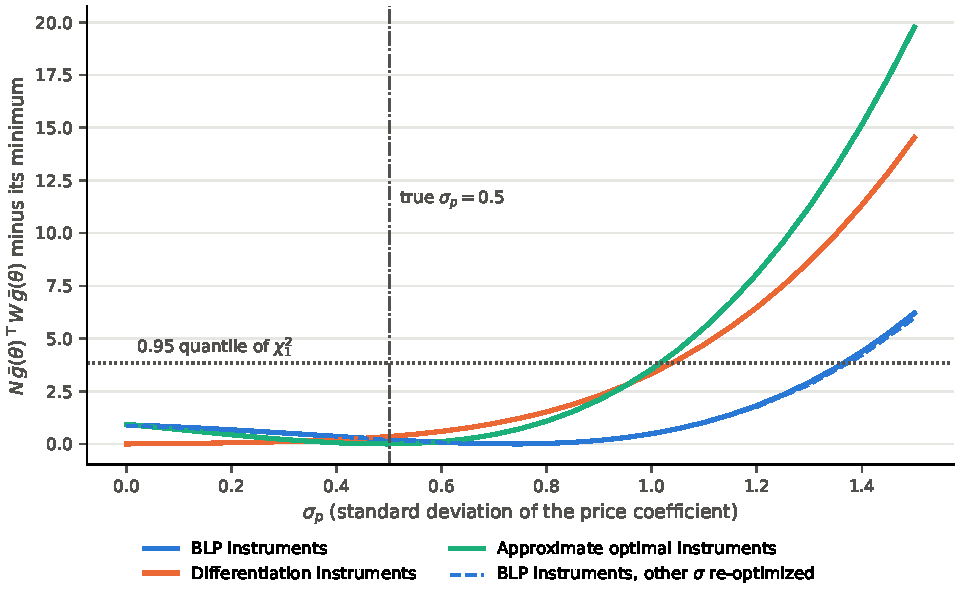
\includegraphics[width=0.92\linewidth]{figures/ch08/sim_profile.pdf}
\caption{The GMM objective as a function of the standard deviation of the price coefficient in the simulated market.
Each solid curve holds the other three standard deviations at the estimate of its instrument set, concentrates out the
linear parameters and uses the second-step weighting matrix. The dashed curve re-optimizes the other three standard
deviations for the BLP instruments. Curves are shifted so that their minimum is zero. The dotted line is the 0.95
quantile of the $\chi^2_1$ distribution, and the dash-dotted line marks the true value $\sigma_p = 0.5$.}
\label{fig:08-profile}
\end{figure}

Why is $\Sigma$ so hard to estimate here? Its identification needs variation that shifts substitution patterns
(\cref{sec:08-instruments}). In this design every product has the same characteristics and the same cost shifter in
every market. The only sources of cross-market variation are the choice set and the prices, and the price of a given
product varies little across markets. Its standard deviation across markets is between 0.045 and 0.061, against 0.189
for all prices together. The inside goods also take only 5 to 21 percent of each market, so most substitution is to
the outside good. Changes in the choice set then move the shares of the remaining products by small amounts, which the
demand shocks, with standard deviation 0.50, easily mask. The simulation correction is small by comparison. It raises
the standard errors by at most 6 percent with the BLP instruments and by less than 1 percent with the other two sets.

The lesson is general. The price coefficient is identified by the cost shifter in every specification, and its
instrumental variables estimates range from 2.5 to 3.5. The standard deviations depend on much weaker variation. A good fit and an
unrejected overidentification test do not certify them. Step 7 shows what is at stake for the substitution patterns.

\subsection{Step 7: elasticities and diversion}\label{sec:08-worked-elas}

We compute the price elasticities of market 0 under each model. Under the random coefficients models we use the
1,000 estimation draws and the recovered mean utilities of that market, and the derivatives of
\cref{prop:08-derivs}. The true elasticities use the true parameters and 200,000 draws, which approximates the
population integral. \Cref{tab:08-sim-elas} reports three objects: the own-price elasticities, the
responses of all shares to the price of product 4, and the diversion ratio to the outside good,
$-\frac{\partial s_0}{\partial p_k}\big(\frac{\partial s_k}{\partial p_k}\big)^{-1}$ (\cref{prop:08-diversion}). Own elasticities are
reported as positive numbers.

\begin{table}[htbp]
\centering
\caption{Elasticities and diversion in market 0.}
\label{tab:08-sim-elas}
\footnotesize
\begin{tabular}{lccccc}
\toprule
 & Logit & \multicolumn{3}{c}{Random coefficients logit} & True \\
\cmidrule(lr){3-5}
 & 2SLS & $\Sigma$ known & \makecell{GMM, approx.\\ optimal IV} & \makecell{GMM,\\ BLP IV} & \\
\midrule
\multicolumn{6}{l}{\emph{A. Own-price elasticity} $-\frac{\partial s_j}{\partial p_j}\frac{p_j}{s_j}$} \\
Product 2 & 3.47 & 3.45 & 3.45 & 3.78 & 3.58 \\
Product 3 & 2.62 & 2.68 & 2.67 & 3.02 & 2.76 \\
Product 4 & 3.70 & 3.63 & 3.64 & 3.42 & 3.77 \\
Product 6 & 2.59 & 2.65 & 2.64 & 2.99 & 2.74 \\
Product 8 & 2.80 & 2.79 & 2.81 & 3.12 & 2.89 \\
Product 9 & 3.81 & 3.74 & 3.74 & 4.01 & 3.87 \\
Product 10 & 2.44 & 2.51 & 2.51 & 2.85 & 2.59 \\
\addlinespace
\multicolumn{6}{l}{\emph{B. Cross-price elasticity with respect to $p_4$,} $\frac{\partial s_j}{\partial p_4}\frac{p_4}{s_j}$} \\
Product 2 & 0.047 & 0.078 & 0.063 & 0.988 & 0.069 \\
Product 3 & 0.047 & 0.067 & 0.059 & 0.038 & 0.060 \\
Product 6 & 0.047 & 0.066 & 0.059 & 0.038 & 0.059 \\
Product 8 & 0.047 & 0.069 & 0.060 & 0.039 & 0.062 \\
Product 9 & 0.047 & 0.079 & 0.064 & 0.978 & 0.070 \\
Product 10 & 0.047 & 0.066 & 0.058 & 0.038 & 0.059 \\
Outside good & 0.047 & 0.043 & 0.044 & 0.032 & 0.040 \\
\addlinespace
\multicolumn{6}{l}{\emph{C. Diversion to the outside good (percent)}} \\
Product 2 & 85.9 & 79.5 & 82.1 & 55.5 & 80.3 \\
Product 3 & 87.7 & 83.4 & 85.2 & 85.7 & 84.0 \\
Product 4 & 86.6 & 80.1 & 82.6 & 64.1 & 80.8 \\
Product 6 & 87.3 & 83.0 & 84.8 & 85.2 & 83.5 \\
Product 8 & 90.6 & 86.7 & 88.4 & 88.9 & 87.2 \\
Product 9 & 86.0 & 79.2 & 81.8 & 55.3 & 80.2 \\
Product 10 & 87.2 & 83.1 & 85.0 & 85.5 & 83.8 \\
\bottomrule
\end{tabular}
\par\smallskip
\parbox{\linewidth}{\footnotesize Notes: Market 0, at observed prices and realized shares. The columns use the
estimates of columns (2), (3), (6) and (4) of \cref{tab:08-sim-demand}. The true values use the true parameters, the
true mean utilities and 200,000 draws. Products 2, 4 and 9 are the organic products and the three most expensive.}
\end{table}

The own elasticities differ little across the logit, the random coefficients model with $\Sigma$ known and the model
estimated with approximate optimal instruments. All three are within 0.15 of the truth, and all are slightly too small
because the estimated price coefficients are below 3. The three most expensive products are the most elastic in every
column. With small shares the logit own elasticity is close to $\alpha p_j$, so this ordering is mechanical in the
logit. In the true model it also holds, because the standard deviation of the price coefficient is moderate.

The cross elasticities separate the models. In the logit, a rise in $p_4$ raises every share, including the outside
share, by the same 0.047 percent per percent. This is the IIA property of \cref{ch:logit}. In the true model the
organic products 2 and 9 gain most (0.069 and 0.070), the other products less (0.059 to 0.062), and the outside good
least (0.040). The model with $\Sigma$ known reproduces this pattern. The model estimated with approximate optimal
instruments shows it only weakly (0.063 and 0.064 against 0.058 to 0.060). Its estimate of $\sigma$ on organic is
zero, so only the random coefficient on price separates the expensive organic products. The model estimated with
BLP instruments gets the pattern badly wrong. Its large $\sigma$ on organic makes products 2 and 9 nearly perfect
substitutes for product 4, with cross elasticities of 0.988 and 0.978, about fourteen times the true values.

Diversion to the outside good tells the same story. The logit sends between 85.9 and 90.6 percent of a product's lost
buyers to the outside good, the value $\frac{s_0}{1 - s_k}$ of \cref{ch:logit}. The true model sends between 80.2 and
87.2 percent, and the models with $\Sigma$ known and with approximate optimal instruments come close. Under the BLP
instrument estimates, only 55 percent of the buyers lost by product 2 or 9 leave the market. Panel B suggests where
the others go: to the other organic products. A merger between the firms that sell products 2 and 9 would look far more harmful
under these estimates than under the true model (\cref{ch:mergers}). \Cref{fig:08-ownelas} summarizes the comparison.

\begin{figure}[htbp]
\centering
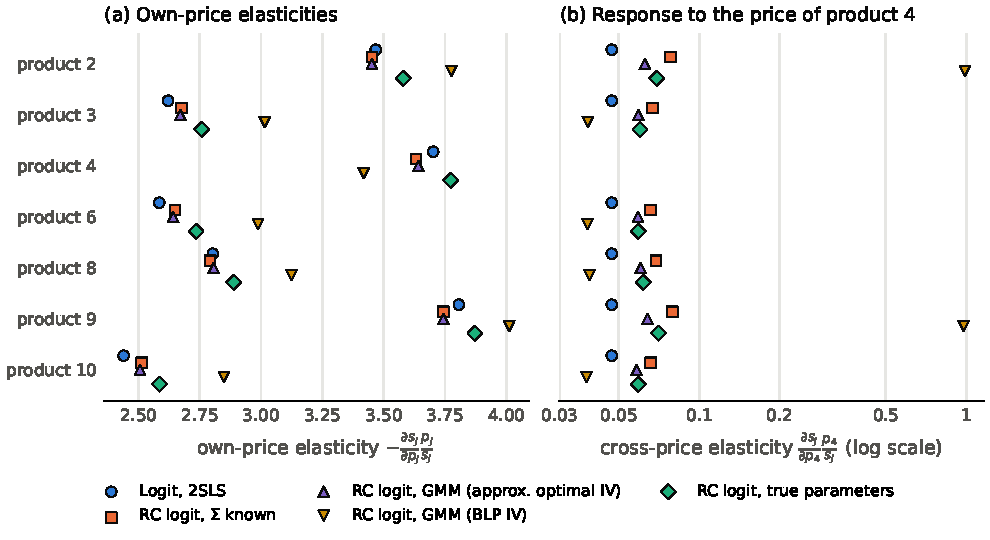
\includegraphics[width=\linewidth]{figures/ch08/sim_ownelas.pdf}
\caption{Elasticities in market 0 of the simulated market. Panel (a) shows own-price elasticities as positive numbers.
Panel (b) shows the cross-price elasticity of each product's share with respect to the price of product 4, on a log
scale. The random coefficients columns use the estimates of \cref{tab:08-sim-demand}, and the true values use 200,000
draws.}
\label{fig:08-ownelas}
\end{figure}

\subsection{What the simulated market teaches}\label{sec:08-worked-lessons}

Four lessons carry over to applications. First, the computational steps are fast and reliable when implemented
carefully. The Morrow-Skerlos iteration finds the equilibrium in 10 to 13 iterations, and the contraction recovers the
mean utilities to $10^{-12}$ in about 15 to 25 iterations. Second, a strong cost shifter identifies the mean price
coefficient well. The logit estimate is biased toward zero by the sorting of less price-sensitive consumers into
expensive products, and the random coefficients model removes most of the bias when $\Sigma$ is right.

Third, $\Sigma$ is the hard part. With market-level data its identification rests on variation in choice sets and in
the characteristics of competing products. When that variation is weak, the estimates of $\Sigma$ and the substitution
patterns they imply can be far from the truth, even when the overidentification test passes. The diagnostics that
reveal the problem are cheap: several starting values, the profile of the objective, the eigenvalues of $G^\top WG$,
and comparisons across instrument sets.

Fourth, the remedies are the subjects of the preceding sections. Richer cross-market variation helps, as do approximate
optimal instruments. Micro moments and second-choice data identify $\Sigma$ from within-market variation
(\cref{sec:08-micro}). A supply side adds moments that depend on $\Sigma$ through the markups (\cref{sec:08-supply}).
Where none of these is available, the appropriate report is the range of substitution patterns consistent with the
data.

\section{Case study: Berry, Levinsohn and Pakes (1995), U.S. automobiles}\label{sec:08-blp95}

\citet{BerryLevinsohnPakes1995}, henceforth BLP, turned the random coefficients logit into a working
tool for industrial organization. They estimate demand and marginal cost for essentially every car
model sold in the United States from 1971 to 1990. They use only product-level data on prices,
quantities and characteristics, together with the distribution of household income. The estimates
come from a model in which consumers choose one car or none and multi-product firms set prices in a
Nash equilibrium.

The general model, its computation and its identification occupy
\cref{sec:08-model,sec:08-substitution,sec:08-simulation,sec:08-inversion,sec:08-gmm,sec:08-instruments,sec:08-supply}.
This section applies that machinery to the paper itself. We follow the order used for every deep case
study in this book. We take up the question, the setting, the data, the model, and the estimator with
its identification. Then come the results, robustness, interpretation, critiques and contribution. We
reproduce the
paper's Tables III, IV, V, VII, VIII and IX in full, Table I in condensed form, and an excerpt of
Table VI. Several derived quantities in this section are our own calculations from the published
tables, and we say so each time.

\subsection{The question and why it matters}\label{sec:08-blp95-question}

The paper asks how to recover demand and cost parameters for a whole differentiated-products industry
when only market-level data are available. The answers must be consistent with an oligopoly
equilibrium. On the demand side BLP want own- and cross-price elasticities for every model, and
elasticities of demand with respect to attributes such as fuel efficiency. On the cost side they want
marginal cost as a function of product characteristics.

These objects are inputs to many policy questions. BLP list trade policy (import restrictions),
merger policy, environmental policy (gas-guzzler and carbon taxes, emission standards and fuel
economy standards) and the construction of price indices (Section 8.1 of the paper). The automobile
market was large, with sales above \$150 billion in 1989 (p.~843). It was also at the center of trade
and environmental debates.

The obvious alternative is a demand system written directly in product space. A constant-elasticity
system for 100 products has 10,000 own- and cross-price elasticities (p.~842). Researchers therefore
aggregate products into groups. BLP point out that a grouping that suits one question rarely suits
another. Aggregating all foreign and all domestic cars may serve a tariff study, but it is useless for
domestic competition or pollution taxes. Product-space systems also cannot predict demand for new
goods, and they make it hard to use information on the distribution of consumers.

BLP work in characteristics space, following \citet{Lancaster1971} and \citet{McFadden1974}. They
identify two problems with the discrete-choice models available at the time. The first is the
functional form of utility, which in logit-type models forces implausible substitution patterns. The
second is the correlation between price and product characteristics that consumers see and the
econometrician does not. BLP call this the differentiated-products analog of the classical
simultaneity problem. They solve the aggregation problem by simulation, as in \citet{Pakes1986}. They
solve the simultaneity problem by inverting the share equations, as in \citet{Berry1994}.

\subsection{Setting and earlier approaches}\label{sec:08-blp95-setting}

Early work treated cars as a homogeneous product and estimated aggregate demand \citep{Suits1958}.
\citet{Griliches1971} introduced hedonic price regressions for cars, which work at the level of the
individual model but do not model the production side. BLP call \citet{Bresnahan1987} perhaps the first
attempt to model and estimate demand and oligopoly pricing jointly (p.~844). He used a vertical differentiation model with a
uniform density of consumers along the quality line (\cref{ch:discrete}).
\citet{FeenstraLevinsohn1995} allowed several dimensions of differentiation but kept the uniform
density. \citet{Manski1983} studied demand and a perfectly competitive supply side for the Israeli car
market.

Micro-data studies of car demand had alternatives to BLP's solutions. They could interact consumer
and product characteristics, or use nested logit, which BLP note is a restricted random coefficients
model on group dummies (p.~851). Nested logit requires a priori knowledge of the order and content of
the nests. Product-specific constants, which would absorb unobserved quality, are hard to estimate with
micro data. There are on average more than 100 products per year in BLP's sample. The Consumer
Expenditure Survey records only about 500 new-car purchases per year (p.~852). Even with product
dummies, one still has to separate the effects of price, observed characteristics and unobserved
quality, which requires the kind of instrumental-variable assumptions BLP make.

The vertical model restricts substitution severely. A product has nonzero cross-price elasticities only
with its two neighbors on the price ladder. BLP give an example with a \$24,998 station wagon, a
\$24,999 sports car and a \$25,000 station wagon (p.~852). The vertical model makes the two wagons
non-substitutes and the sports car a substitute for both. The logit model fails in the opposite way.
If a cheap Yugo and an expensive Mercedes have the same share, a rise in the BMW's price must raise
both of their sales by the same amount (p.~847). Two products with equal shares must also have equal
own-price derivatives, and hence equal markups under single-product pricing
(\cref{sec:08-substitution}).

Finally, BLP stress the structural error $\xi_{jt}$. Without it, only sampling error separates the
model's predicted shares from the data. With aggregate samples of millions of households, a
chi-square test of the model's restrictions on the multinomial shares rejects with probability close
to one (p.~850). The unobserved characteristic plays the role of the demand disturbance in
homogeneous-goods markets. Because firms know it when they set prices, prices are correlated with it.

\subsection{Data}\label{sec:08-blp95-data}

The unit of observation is a car model in a year, and a market is the national market in a year.
Product characteristics come from annual issues of the \emph{Automotive News Market Data Book},
combined with a similar data set from Ernst Berndt (p.~868). The sample covers essentially all models
sold from 1971 to 1990. Only ``exotic'' models with tiny shares, such as Ferrari and Rolls Royce, are
excluded. The panel is unbalanced because models enter and exit. It has 2,217 model-years.

BLP need a rule that links model-years into models, because their standard errors allow correlation
within a model over time. Two observations in adjacent years are the same model if they have the same
name and their horsepower, width, length and wheelbase each change by at most ten percent. With this
rule the 2,217 model-years represent 997 distinct models (p.~869).

The variables are as follows.
\begin{itemize}
\item \emph{Price} is the list retail price of the base model, in thousands of 1983 dollars (deflated
  by the CPI). BLP would prefer transaction prices but could not find them.
\item \emph{Quantity} is U.S. sales by nameplate, in thousands. Fleet sales are not observed, so fleet
  buyers are treated as agents of households (footnote 23).
\item \emph{HPWT} is horsepower divided by weight, in horsepower per 10 pounds.
\item \emph{Air} equals one if air conditioning is standard equipment.
\item \emph{MP\$} (miles per dollar) is the EPA miles-per-gallon rating divided by the real price of
  unleaded gasoline. It measures the cost of driving and enters utility. The production cost of fuel
  efficiency is captured instead by \emph{MPG}, which enters the cost function.
\item \emph{Size} is length times width.
\item \emph{Reliability} is the Consumer Reports rating from 1 to 5, available for part of the sample
  and rescaled every year (footnote 24). It appears only in one robustness check.
\end{itemize}
The market size $M_t$ is the number of U.S. households in year $t$, from the \emph{Statistical
Abstract}. The parameters of the household income distribution come from the March Current Population
Survey (CPS) for each year. Divisions of one parent company form one firm, so Buick, Cadillac,
Chevrolet, Oldsmobile and Pontiac all belong to General Motors. There are 22 firms (footnote 29). Each
model is assigned the country of its producing firm.

\begin{table}[htbp]
\centering
\caption{Descriptive statistics of the BLP (1995) data, selected years (condensed from their Table I)}
\label{tab:08-blp-desc}
\footnotesize
\setlength{\tabcolsep}{3.6pt}
\begin{tabular}{@{}lrrrrrrrrrrr@{}}
\toprule
Year & Models & Quantity & Price & Domestic & Japan & Europe & HPWT & Size & Air & MPG & MP\$ \\
\midrule
1971 & 92  & 86.892  & 7.868  & 0.866 & 0.057 & 0.077 & 0.490 & 1.496 & 0.000 & 1.662 & 1.850 \\
1973 & 86  & 92.785  & 7.535  & 0.932 & 0.040 & 0.028 & 0.364 & 1.529 & 0.022 & 1.589 & 1.819 \\
1974 & 72  & 105.119 & 7.506  & 0.887 & 0.050 & 0.064 & 0.347 & 1.510 & 0.026 & 1.568 & 1.453 \\
1975 & 93  & 84.775  & 7.821  & 0.853 & 0.083 & 0.064 & 0.337 & 1.479 & 0.054 & 1.584 & 1.503 \\
1980 & 103 & 71.567  & 7.718  & 0.773 & 0.191 & 0.036 & 0.350 & 1.296 & 0.078 & 2.215 & 1.466 \\
1985 & 136 & 78.143  & 8.938  & 0.761 & 0.191 & 0.048 & 0.372 & 1.265 & 0.140 & 2.261 & 2.024 \\
1988 & 150 & 67.078  & 10.069 & 0.717 & 0.237 & 0.045 & 0.396 & 1.251 & 0.237 & 2.334 & 2.919 \\
1990 & 131 & 66.377  & 10.337 & 0.682 & 0.276 & 0.043 & 0.419 & 1.270 & 0.308 & 2.270 & 2.852 \\
\midrule
All  & 2217 & 78.804 & 8.604  & 0.790 & 0.161 & 0.049 & 0.372 & 1.357 & 0.116 & 2.099 & 2.086 \\
\bottomrule
\end{tabular}

\smallskip
\begin{minipage}{0.97\linewidth}
\footnotesize
Notes: Source: \citet{BerryLevinsohnPakes1995}, Table I (p.~870), which reports all 20 years.
``Models'' is the number of models and ``Quantity'' is mean sales per model. The remaining nine columns
are sales-weighted means. Quantity is in thousands of cars and price in thousands of 1983 dollars. HPWT
is in horsepower per 10 pounds, MPG in tens of miles per gallon and MP\$ in tens of miles per 1983 dollar
of gasoline. Domestic, Japan and Europe are
dummies for the location of the producing firm's headquarters.
\end{minipage}
\end{table}

\Cref{tab:08-blp-desc} shows the main trends. The number of models rose from a low of 72 in 1974 to a
high of 150 in 1988, while sales per model trended down. The sales-weighted list price stayed between
about \$7,500 and \$8,000 during the 1970s. It then rose from \$7,718 in 1980 to \$10,337 in 1990, about a
third.\footnote{The text of \citet[p.~870]{BerryLevinsohnPakes1995} says that the real sales-weighted list price
``has risen almost 50 percent during the 1980's.'' Their Table I, which is already in 1983 dollars, implies an
increase of $\frac{10.337}{7.718} - 1 = 34$ percent from 1980 to 1990. Measured from the 1979 value of 7.599, the
increase is 36 percent. We follow the table.} The characteristics changed at the same time, so the price of a fixed bundle need not have
risen. HPWT fell in the early 1970s and then trended up, mostly because cars became lighter. Fuel cost
efficiency improved, from 18.50 miles per 1983 dollar of gasoline in 1971 to 28.52 in 1990. Air
conditioning was standard on no car at the start and on 30.8 percent at the end. The domestic share
fell from a 1973 high of 93.2 percent to 68.2 percent in 1990, while the Japanese share rose from 4.0 to
27.6 percent.

BLP's Table II reports quartiles of the continuous variables and names the models at each quartile.
The cheapest car is the 1990 Yugo at \$3,393 (1983 dollars). The median price is \$8,728 and the 75th
percentile is \$13,074. The most expensive car is a 1989 Porsche 911 Cabriolet at \$68,597. Sales range
from 49 cars to 577,313 cars (the 1971 Chevrolet Impala), with a median of 47,345. MPG ranges from 9
(1974 Cadillac Eldorado) to 53 (1989 Geo Metro). We use the price quartiles below to interpret the
logit results.

The data also pin down the size of the outside good. Total 1990 sales are about
$131\times 66.377\approx 8{,}695$ thousand cars (\cref{tab:08-blp-desc}). BLP describe the logit column
of their Table VII as $\frac{s_0}{1-s_j}$, and its entries lie between 90.458 and 90.883 percent.
Because $\frac{s_0}{1-s_j}$ exceeds $s_0$, the smallest entry bounds the outside share, $s_0 < 0.9046$.
The entries do not rise with the shares as the formula requires (the best-selling Accord has the
smallest entry), so we read them only as $s_0 \approx 0.90$. With $s_0$ near 0.90,
$M_{1990}=\frac{8.695}{1-s_0}$ is roughly 90 million households (our calculation). Most households do not buy a new car in a given year, so the outside good is large.

\subsection{The model}\label{sec:08-blp95-model}

\casehead{Utility}
BLP nest random coefficients in the Cobb-Douglas utility \eqref{eq:08-cobb-douglas} over the car's
characteristics and spending on other goods (their eq.~2.6). Its logarithm gives the inside and outside
utilities \eqref{eq:08-blp-inside} and \eqref{eq:08-blp-outside} (their eqs.~2.7a and 2.7b), which
\cref{sec:08-income} derived. BLP write $\bar\beta$ for our $\beta$. The taste shocks $\nu_{ik}$ have mean
zero and unit variance, so characteristic $k$ has marginal utility $\beta_k+\sigma_k\nu_{ik}$, with mean
$\beta_k$ and variance $\sigma_k^2$. The term $\sigma_0\nu_{i0}$ lets the outside option have more
idiosyncratic variance than the inside goods. BLP motivate it by unobserved differences in access to
public transport and in used-car holdings (p.~849).

BLP prefer this form to the plain random coefficients model
$u_{ij}=x_j\beta-\alpha p_j+\xi_j+\sum_k\sigma_kx_{jk}\nu_{ik}+\epsilon_{ij}$ (their eq.~2.5) for two
reasons (p.~848). They have outside information on the income distribution, and they have a
theoretical rationale for the form of the interaction between income and price. The Cobb-Douglas form
uses both.

\casehead{The estimated form}
The empirical model adds a year index $t$ and makes income random. Household income is lognormal,
$y_{it}=e^{m_t+\sigma_y\nu_{iy}}$, with year-specific mean $m_t$ and a common standard deviation
$\sigma_y$, both estimated from the CPS. The utility functions are \eqref{eq:08-blp-final-inside} and
\eqref{eq:08-blp-final-outside} (their eqs.~6.14a and 6.14b). The vector
$(\nu_{iy},\nu_{i0},\nu_{i1},\dots,\nu_{iK})$ is standard multivariate normal, independent of everything
else. BLP hold each simulated consumer's draws fixed over the 20 years of the panel. The idiosyncratic
shocks $\epsilon_{ijt}$ are \iid\ type-I extreme value. BLP did not estimate a separate $\sigma_y$ for each
year because those estimates were imprecise. They also tried drawing incomes directly from the CPS, which
gave imprecise simulators, especially in the upper tail (footnote 21).

The characteristics in utility are $x_{jt}=(1,\mathit{HPWT}_{jt},\mathit{Air}_{jt},
\mathit{MP\$}_{jt},\mathit{Size}_{jt})$, so $K=5$. Each has a mean $\beta_k$ and a standard deviation
$\sigma_k$. Price carries no separate random coefficient. Heterogeneity in price sensitivity comes
entirely from income, as we now show.

\casehead{Mean utility and individual deviations}
Choice probabilities depend only on utility differences, so we subtract \eqref{eq:08-blp-final-outside} from
\eqref{eq:08-blp-final-inside} and normalize $\xi_{0t}=0$. The deterministic part of the difference is
\begin{align*}
u_{ijt}-u_{i0t}-(\epsilon_{ijt}-\epsilon_{i0t})
 &=\alpha\big[\ln(y_{it}-p_{jt})-\ln y_{it}\big]+x_{jt}\beta+\xi_{jt}
   +\sum_k\sigma_kx_{jkt}\nu_{ik}-\sigma_0\nu_{i0}\\
 &=\underbrace{x_{jt}\beta+\xi_{jt}}_{\delta_{jt}}
   +\underbrace{\alpha\ln\Big(1-\frac{p_{jt}}{y_{it}}\Big)+\sum_k\sigma_kx_{jkt}\nu_{ik}
   -\sigma_0\nu_{i0}}_{\mu_{ijt}} .
\end{align*}
Three features of this decomposition matter for estimation. First, the mean utility
\begin{equation}\label{eq:08-blp-delta}
\delta_{jt}=x_{jt}\beta+\xi_{jt}
\end{equation}
contains no price term. Price enters only through $\mu_{ijt}$, so $\alpha$ is a nonlinear parameter.
In the chapter's notation $\theta_1=\beta$ and $\theta_2=(\alpha,\sigma_1,\dots,\sigma_5)$. Second, the
constant is the first characteristic ($x_{j1t}=1$), so the terms $\sigma_1\nu_{i1}-\sigma_0\nu_{i0}$
combine into one normal random variable with variance $\sigma_1^2+\sigma_0^2$. A random coefficient on
the inside-good constant and an extra shock on the outside good are therefore observationally
equivalent, and only the combined variance is identified. This is why BLP's footnote 6 describes
$\sigma_0\nu_{i0}$ as a random coefficient on the constant. The reported standard deviation on the
constant measures this combined dispersion. Third,
$\mu_{ijt}$ is defined only when $y_{it}>p_{jt}$. A simulated household whose income draw is below a
car's price cannot buy that car, and an implementation must remove the car from that household's
choice set.

\casehead{Market shares}
Conditional on $\nu_i$, integrating the extreme value shocks gives the logit form
\eqref{eq:08-individual-share} (their eq.~6.6). The market share \eqref{eq:08-share-integral} integrates over the
standard normal vector $\nu_i$, with income determined by $\nu_{iy}$ (their eq.~6.7). The inner integral has a
closed form and the outer one does not. BLP evaluate it by simulation (\cref{sec:08-simulation}).

\casehead{Price derivatives and elasticities}
Differentiating $\mu_{ijt}$ gives the price sensitivity of household $i$ for car $j$:
\begin{equation*}
\frac{\partial\mu_{ijt}}{\partial p_{jt}}=-\frac{\alpha}{y_{it}-p_{jt}} .
\end{equation*}
This sensitivity falls with income. It also rises with the car's own price, because a dollar is
worth more when less is left for other goods. A first-order expansion of the log for small
$\frac{p_{jt}}{y_{it}}$ gives
\begin{equation*}
\alpha\ln\Big(1-\frac{p_{jt}}{y_{it}}\Big)\approx-\alpha\,\frac{p_{jt}}{y_{it}},
\end{equation*}
so household $i$ behaves approximately as if its price coefficient were $\frac{\alpha}{y_{it}}$.
Applying the general derivative formulas of \cref{prop:08-derivs} with this price sensitivity gives
\begin{align}
\frac{\partial s_{jt}}{\partial p_{jt}}&=-\int\frac{\alpha}{y_{it}-p_{jt}}\,
  s_{ijt}(1-s_{ijt})\,\dd F(\nu_i),\label{eq:08-blp-dsown}\\
\frac{\partial s_{jt}}{\partial p_{qt}}&=\int\frac{\alpha}{y_{it}-p_{qt}}\,s_{ijt}s_{iqt}\,
  \dd F(\nu_i),\qquad q\neq j\label{eq:08-blp-dscross}
\end{align}
(their eqs.~6.9a and 6.9b). The derivative of the outside share is
$\frac{\partial s_{0t}}{\partial p_{qt}}=\int\frac{\alpha}{y_{it}-p_{qt}}s_{i0t}s_{iqt}\,\dd F(\nu_i)$.

BLP report \emph{semi-elasticities}, which we denote
\begin{equation}\label{eq:08-blp-semi}
e_{jq}\equiv\frac{100}{s_j}\,\frac{\partial s_j}{\partial p_q},
\end{equation}
with prices in thousands of dollars. The entry $e_{jq}$ is the percentage change in the share of $j$
when the price of $q$ rises by \$1,000. The elasticity follows by multiplying by
$\frac{p_q}{100}$, so the own-price elasticity, written as a positive number, is
$\varepsilon_j=-\frac{p_j}{100}\,e_{jj}$. The logit benchmark has $e_{jj}=-100\,\alpha(1-s_j)$ and
$e_{jq}=100\,\alpha s_q$.

\casehead{Costs and pricing}
Firm $f$ produces the set $\mathcal{J}_f$ of models. Marginal cost is constant in output and log-linear
in observed cost characteristics $w_j$ and an unobserved cost shock $\omega_j$:
\begin{equation}\label{eq:08-blp-mc}
\ln mc_j=w_j\gamma+\omega_j
\end{equation}
(their eq.~3.1). The cost characteristics are a constant, $\ln\mathit{HPWT}$, $\mathit{Air}$,
$\ln\mathit{MPG}$, $\ln\mathit{Size}$ and a time trend. MPG replaces MP\$ because the production cost
of fuel efficiency does not depend on the retail price of gasoline, at least in the short run. The
trend captures technical change and regulation. Logs of the continuous attributes make the cost
coefficients elasticities of marginal cost. BLP allow $\omega_j$ to be correlated with $\xi_j$, since
cars with more unobserved quality may cost more to build.

Firm $f$'s profit is \eqref{eq:08-profit} (their eq.~3.2), and each firm chooses its prices given rivals'
prices. An interior Nash equilibrium satisfies the first-order conditions \eqref{eq:08-foc} (their eq.~3.3).
\Cref{sec:08-supply-foc} showed that BLP's markup formula (their eqs.~3.4 and 3.5) is our
\eqref{eq:08-markup}, and that substituting it into \eqref{eq:08-blp-mc} gives the pricing equation
\eqref{eq:08-pricing-log} (their eq.~3.6). The markup depends on $\omega$ through the equilibrium prices, and on
$\xi$ directly. It therefore cannot be treated as exogenous in the pricing equation.

BLP assume that a Nash equilibrium exists with prices in the interior of the positive orthant
(footnote 12). The existence results of \citet{CaplinNalebuff1991} cover single-product firms and do
not extend easily to multi-product firms. BLP instead check existence numerically at their estimates.
None of the properties of the estimator requires a unique equilibrium. Without uniqueness, however, it
is not clear how to use the estimates for policy counterfactuals.

\subsection{Estimation and identification}\label{sec:08-blp95-estimation}

\casehead{Moment conditions}
Let $z_j=(x_j,w_j)$ collect the demand and cost characteristics of product $j$, and let
$z=(z_1,\dots,z_J)$ collect them for all products in the market. BLP's identifying assumption is
\begin{equation}\label{eq:08-blp-moments}
\E[\xi_j\mid z]=\E[\omega_j\mid z]=0
\end{equation}
(their eq.~4.1). Prices and quantities are excluded from the conditioning set because the model
determines them partly through $\xi$ and $\omega$. Characteristics and cost shifters are treated as
predetermined because the model does not explain how they are chosen.

BLP acknowledge that \eqref{eq:08-blp-moments} holds only if the true process that chooses
characteristics has special properties (p.~854). They mention an alternative for panel data. The
pair $(\xi,\omega)$ of a model could follow a first-order Markov process whose innovations are
independent of the model's initial characteristics. This assumption would also identify the model, but
it would demand much more of the data, so BLP start from \eqref{eq:08-blp-moments}.

\casehead{Why characteristics of other products are instruments}
Under \eqref{eq:08-blp-moments}, any function of $z$ is a valid instrument. The question is which
functions carry information. BLP's answer comes from oligopoly pricing (p.~855). Products that face
close substitutes have low markups, so the characteristics of rival products shift a product's price.
Nash markups respond differently to products of the same firm and to products of rivals. The
instruments should therefore distinguish the two. The demand for $j$ depends on the characteristics of
all products, so no characteristic is excluded from the demand of $j$ in the usual sense. What
identifies demand is the restriction that the utility of $j$ depends only on the characteristics of
$j$. The number of utility parameters then grows with the number of characteristics, and not with the
number of products.

\casehead{The instrument vector}
The efficient instruments under conditional moment restrictions are infeasible here
(\cref{sec:08-optiv}). BLP instead use the first-order terms \eqref{eq:08-blp-iv} of a partially
exchangeable basis (their eq.~5.8). These are the own characteristic, its sum over the firm's other products
and its sum over rival products. \Cref{sec:08-optiv} derives this basis from the exchangeability of a
unique Nash equilibrium \citep{Pakes1994}. The two sums vary across products because they exclude different
own products, because firms offer different sets of products, and because the set of products changes over
time. The constant is one of the characteristics, so the numbers of own-firm and rival products are
instruments too.

Higher-order basis functions were nearly collinear with the first-order terms, and even the first-order
terms were nearly of reduced rank. For the demand error BLP use the three terms of
\eqref{eq:08-blp-iv} for each of the five demand characteristics, giving 15 instruments. MPG and the
trend enter cost and not demand, so they are excluded from demand. Adding them to the demand list caused
numerical problems through near collinearity, and BLP left them out. For the cost error BLP use the three terms for each of the six cost characteristics,
plus MP\$, giving 19 instruments. The estimator therefore uses $15+19=34$ moment conditions (p.~862).
There are 17 parameters: five means $\beta$, five standard deviations $\sigma$, the income coefficient
$\alpha$ and six cost parameters $\gamma$. Hence there are 17 overidentifying restrictions.

BLP enter the basis functions directly as GMM instruments, instead of first projecting the optimal
instruments on them as \citet{Newey1990} suggests (\cref{sec:08-optiv}).

\casehead{Clustering by model}
Disturbances of the same model in different years are likely to be more similar than those of
different models. BLP therefore treat the sum of a model's moments over the years it is sold as one
draw from an exchangeable population of models. Let $z^d_{mt}$ and $z^s_{mt}$ be the 15 demand and 19
cost instruments of model $m$ in year $t$, and let $\mathcal{T}_m$ be the years in which $m$ is sold.
The moment contribution of model $m$ is
\begin{equation}\label{eq:08-blp-gm}
g_m(\theta)=\sum_{t\in\mathcal{T}_m}\begin{pmatrix} z^{d\T}_{mt}\,\xi_{mt}(\theta)\\
z^{s\T}_{mt}\,\omega_{mt}(\theta)\end{pmatrix}\in\R^{34}.
\end{equation}
BLP write this as $\sum_t[f_{mt}(z)^{\T}\otimes I_2](\xi_{mt},\omega_{mt})^{\T}$, with the
instrument blocks restricted as described above. The estimator minimizes
\begin{equation}\label{eq:08-blp-obj}
Q(\theta)=\bar g(\theta)^{\T}\,W\,\bar g(\theta),\qquad
\bar g(\theta)=\frac{1}{997}\sum_{m=1}^{997}g_m(\theta),
\end{equation}
with $W$ a consistent estimate of the inverse covariance matrix of $g_m$. The resulting standard errors
allow arbitrary correlation across years within a model and arbitrary heteroskedasticity across
models. BLP note that this is probably not the most efficient way to use the panel.

\casehead{Computing the objective}
Each evaluation of the moments takes four steps for a given $\theta$ (p.~863).
\begin{enumerate}
\item Simulate the market shares $s_{jt}(\delta_t;\theta_2)$ implied by the model.
\item Solve for the mean utilities $\delta_t$ that equate simulated and observed shares, and set
  $\xi_{jt}=\delta_{jt}-x_{jt}\beta$.
\item Compute the markups $b_{jt}$ from the simulated share derivatives and set
  $\omega_{jt}=\ln(p_{jt}-b_{jt})-w_{jt}\gamma$.
\item Interact $\xi$ and $\omega$ with the instruments to form \eqref{eq:08-blp-gm}.
\end{enumerate}
The logit benchmark puts price in the mean utility, $\delta_{jt}=x_{jt}\beta-\alpha p_{jt}+\xi_{jt}$, and
sets $\mu_{ijt}=0$. Every step is then analytic. Shares are
$s_{jt}=\frac{e^{\delta_{jt}}}{1+\sum_qe^{\delta_{qt}}}$, the inversion is
$\delta_{jt}=\ln s_{jt}-\ln s_{0t}$, and the demand error is
$\xi_{jt}=\ln s_{jt}-\ln s_{0t}-x_{jt}\beta+\alpha p_{jt}$ (their eqs.~6.3 to 6.5). In the full model
step~2 uses the contraction
\begin{equation*}
\delta_{jt}^{h+1}=\delta_{jt}^{h}+\ln s^{\text{obs}}_{jt}-\ln s_{jt}\big(\delta_t^{h};\theta_2\big)
\end{equation*}
(their eq.~6.8), whose convergence BLP prove in their Appendix~I (\cref{thm:08-contraction}).

Step~1 uses the importance sampler \eqref{eq:08-blp-importance} of \cref{sec:08-importance} (their
eq.~6.13). BLP first obtain a preliminary estimate $\theta'$ with the plain smooth simulator. They then
accept population draws of $\nu$ with probability $\bar f(\nu;\theta')$, the probability that a household
with tastes $\nu$ buys some car, and reweight each accepted draw by $\frac{\bar s(\theta')}{\bar
f(\nu;\theta')}$. The sampler oversamples households likely to buy a car, which is where the integrand is
large. The same draws are used for every share, so the simulated shares sum to one, as the contraction
requires.

The first-order conditions of \eqref{eq:08-blp-obj} are linear in $\beta$ and $\gamma$ given
$(\alpha,\sigma)$. Both $\xi=\delta(\theta_2)-X\beta$ and $\omega=\ln(p-b(\theta_2))-W_c\gamma$ are linear
in the linear parameters, where $W_c$ stacks the $w_{jt}$. The markup depends only on $\theta_2$ because
it is computed from the inverted $\delta$ and the share derivatives. BLP concentrate out $\beta$ and
$\gamma$ as in \cref{prop:08-concentrate} and search over the six elements of $(\alpha,\sigma)$ with the
\citet{NelderMead1965} simplex method (p.~868).

\casehead{Standard errors}
The asymptotic variance is \eqref{eq:08-blp-avar}, the sandwich with the three variance pieces $V_1$
(product characteristics), $V_2$ (consumer sampling) and $V_3$ (simulation) derived in
\cref{sec:08-asymptotics}. With about 100 million U.S. households, $V_2$ is negligible and $V_3$ is not.
BLP estimate $V_3$ by redrawing the simulation draws. The correction raises the standard errors in their
Table IV by about 5 to 20 percent, except for one parameter whose standard error doubles (p.~859).

\casehead{What identifies the parameters}
Four sources of information identify the model. The cross-section of mean utilities, together with the
characteristics instruments, identifies $\beta$ and the overall level of price sensitivity. The CPS
income distribution fixes how price sensitivity varies across households, up to the single parameter
$\alpha$. The standard deviations $\sigma_k$ are identified by how shares respond to the configuration
of products in characteristics space. BLP explain the distinction between a mean and a variance with
HPWT (p.~877). Cars with high HPWT can be popular because the mean taste for HPWT is high, or because
the taste is dispersed and some consumers value HPWT a lot. Both raise the share of high-HPWT cars.
They have different implications for substitution. With dispersed tastes, consumers who leave a
high-HPWT car are those who value HPWT most, so they move disproportionately to other high-HPWT cars.

The panel helps here. BLP report that separating means from variances was much harder in a single
cross section than in the panel, which was one reason to use twenty years of data (footnote 30). The
supply side adds a fourth source. The markups in \eqref{eq:08-markup} depend on $\theta_2$, so the
cost moments carry information about demand (\cref{sec:08-supply}). BLP note that their use of
``identification'' is informal and that a formal argument would need further regularity conditions
(footnote 13). \Cref{sec:08-instruments} discusses what later work established.

\subsection{Results I: logit benchmarks}\label{sec:08-blp95-logit}

BLP first estimate two logit models and a marginal-cost pricing regression. The logit models give a
transparent reference point. They also isolate the effect of instrumenting for price, because the IV
logit keeps the logit's substitution patterns. \Cref{tab:08-blp-logit} reproduces their Table III.

\begin{table}[htbp]
\centering
\caption{Logit demand and marginal-cost pricing, 2,217 observations (BLP 1995, Table III)}
\label{tab:08-blp-logit}
\small
\begin{tabular}{@{}lccc@{}}
\toprule
 & OLS logit & IV logit & OLS $\ln(\text{price})$ \\
Variable & demand & demand & on $w$ \\
\midrule
Constant & $-10.068$ & $-9.273$ & 1.882 \\
         & (0.253) & (0.493) & (0.119) \\
HPWT$^{*}$ & $-0.121$ & 1.965 & 0.520 \\
         & (0.277) & (0.909) & (0.035) \\
Air      & $-0.035$ & 1.289 & 0.680 \\
         & (0.073) & (0.248) & (0.019) \\
MP\$     & 0.263 & 0.052 & \\
         & (0.043) & (0.086) & \\
MPG$^{*}$ & & & $-0.471$ \\
         & & & (0.049) \\
Size$^{*}$ & 2.341 & 2.355 & 0.125 \\
         & (0.125) & (0.247) & (0.063) \\
Trend    & & & 0.013 \\
         & & & (0.002) \\
Price    & $-0.089$ & $-0.216$ & \\
         & (0.004) & (0.123) & \\
\midrule
No.\ of inelastic demands & 1494 & 22 & n.a. \\
(at $\pm 2$ s.e.) & (1429--1617) & (7--101) & \\
$R^2$ & 0.387 & n.a. & 0.656 \\
\bottomrule
\end{tabular}

\smallskip
\begin{minipage}{0.86\linewidth}
\footnotesize
Notes: Source: \citet{BerryLevinsohnPakes1995}, Table III (p.~873). Standard errors in
parentheses. The dependent variable in the demand columns is $\ln s_{jt}-\ln s_{0t}$. Starred
continuous characteristics enter demand in levels and the price regression in logs. The IV logit uses
the instruments of \eqref{eq:08-blp-iv}. Column 3 assumes marginal-cost pricing.
\end{minipage}
\end{table}

\casehead{OLS logit}
The first column regresses $\ln s_{jt}-\ln s_{0t}$ on the characteristics and price by OLS. The
coefficients on HPWT and Air are negative but imprecise, which BLP call anomalies.\footnote{The text
on p.~872 names ``air conditioning and size'' as the variables with negative coefficients. In the
printed table the negative coefficients are on HPWT and Air, while Size has a positive coefficient of
2.341. We follow the table.} The price coefficient of $-0.089$ implies that 1,494 of the 2,217 models
have inelastic demand.

This count follows directly from the logit formula. The logit own elasticity is
$\varepsilon_j=\alpha p_j(1-s_j)$, and inside shares are tiny, so demand is inelastic when
\begin{equation*}
\alpha p_j(1-s_j)<1
\iff p_j<\frac{1}{\alpha(1-s_j)}\approx\frac{1}{\alpha}.
\end{equation*}
With $\alpha=0.089$ the cutoff is $\frac{1}{0.089}\approx 11.24$, or \$11,236. The median price in
BLP's Table II is \$8,728 and the 75th percentile is \$13,074. Between half and three quarters of all
model-years should therefore be inelastic, and the reported count is 1,494, or 67 percent. The same
calculation at $\alpha\pm2(0.004)$ gives cutoffs of \$10,309 and \$12,346, which bracket the reported
range of 1,429 to 1,617 inelastic demands (our calculation).

Inelastic demand is inconsistent with profit maximization. A single-product firm sets
$\frac{p_j-mc_j}{p_j}=\frac{1}{\varepsilon_j}$, which is below one only if $\varepsilon_j>1$.
\Cref{prop:08-blp-lerner} below shows that the same requirement holds for multi-product firms. The OLS
estimate is therefore implausible on economic grounds, and BLP show that its imprecision does not
explain the problem.

\casehead{IV logit}
The second column instruments price with the characteristics-based instruments. Every characteristic
now enters utility positively, and all but MP\$ are significant. The price coefficient more than
doubles in absolute value, from $-0.089$ to $-0.216$. This is what the simultaneity story predicts:
products with high unmeasured quality sell at high prices, so OLS attributes part of the quality to a
weak price response. Only 22 models now have inelastic demand. The cutoff falls to
$\frac{1}{0.216}\approx 4.63$, or \$4,630, and the cheapest car in the sample costs \$3,393, so few
models can lie below it.\footnote{The reported range of 7 to 101 inelastic demands at $\pm2$ standard
errors cannot come from the printed standard error of 0.123 in the simple way used for the OLS column.
That interval, $0.216\pm0.246$, includes zero and negative values. The paper does not explain the
calculation, and we report the table as printed.}

The fit of the logit regression shows that unobserved characteristics are large. The OLS logit has
$R^2=0.387$, so $1-0.387=61$ percent of the variance in mean utility levels is due to $\xi$ (p.~874).

\casehead{The logit's markups}
The logit cannot generate plausible markups. The IV logit implies that all 1990 models have markups
between \$4,630 for the BMW and \$4,805 for the Chevrolet Cavalier (p.~874). GM, which sells the most
models, has the highest markups, and BMW, which sells the fewest, has the lowest.
\Cref{prop:08-logit-markup} explains why. Under the logit every product of firm $f$ has the dollar markup
$\frac{1}{\alpha(1-S_f)}$, where $S_f$ is the firm's combined share.

With $\alpha=0.216$, a firm with a negligible combined share has markup $\frac{1}{0.216}\approx4.630$
thousand dollars. This is exactly BMW's reported \$4,630. GM's \$4,805 implies
$1-S_{GM}=\frac{1}{0.216\times4.805}$, so GM's combined market share was about $3.6$ percent of
households in 1990 (our calculation). The logit therefore ties markups to the size of a firm's portfolio and to nothing
else. A Yugo and a BMW sold by firms of equal size would have identical dollar markups. BLP report that
putting $\ln p$ in place of $p$ in the logit makes markups more reasonable, but substitution remains
unreasonable (footnote 26).

\casehead{Marginal-cost pricing}
The third column assumes $p=mc$ and regresses $\ln p_j$ on $w_j$, which is a hedonic price regression.
All characteristics except MPG have positive and significant coefficients. A 10 percent increase in
HPWT is associated with a 5.2 percent increase in price, and hence in marginal cost under this
assumption. The $R^2$ of 0.656 is much higher than that of the logit demand equation. Simple functions
of characteristics explain log prices far better than they explain mean utilities (p.~875).

\subsection{Results II: parameters of the full model}\label{sec:08-blp95-params}

\Cref{tab:08-blp-full} reproduces BLP's Table IV. The first pair of columns imposes constant returns to
scale (CRTS). The second adds $\ln q_j$ to the cost function. The standard errors are corrected for
simulation error and for correlation within models over time, but not for correlation across models
(p.~875).

\begin{table}[htbp]
\centering
\caption{Demand and pricing equations, BLP specification, 2,217 observations (BLP 1995, Table IV)}
\label{tab:08-blp-full}
\small
\begin{tabular}{@{}llcccc@{}}
\toprule
 & & \multicolumn{2}{c}{Constant returns} & \multicolumn{2}{c}{With $\ln q$ in cost} \\
\cmidrule(lr){3-4}\cmidrule(l){5-6}
Parameters & Variable & Estimate & S.e. & Estimate & S.e. \\
\midrule
Means ($\beta$) & Constant & $-7.061$ & 0.941 & $-7.304$ & 0.746 \\
 & HPWT & 2.883 & 2.019 & 2.185 & 0.896 \\
 & Air & 1.521 & 0.891 & 0.579 & 0.632 \\
 & MP\$ & $-0.122$ & 0.320 & $-0.049$ & 0.164 \\
 & Size & 3.460 & 0.610 & 2.604 & 0.285 \\
\addlinespace
Std.\ deviations ($\sigma$) & Constant & 3.612 & 1.485 & 2.009 & 1.017 \\
 & HPWT & 4.628 & 1.885 & 1.586 & 1.186 \\
 & Air & 1.818 & 1.695 & 1.215 & 1.149 \\
 & MP\$ & 1.050 & 0.272 & 0.670 & 0.168 \\
 & Size & 2.056 & 0.585 & 1.510 & 0.297 \\
\addlinespace
Term on price ($\alpha$) & $\ln(y-p)$ & 43.501 & 6.427 & 23.710 & 4.079 \\
\addlinespace
Cost side ($\gamma$) & Constant & 0.952 & 0.194 & 0.726 & 0.285 \\
 & $\ln$ HPWT & 0.477 & 0.056 & 0.313 & 0.071 \\
 & Air & 0.619 & 0.038 & 0.290 & 0.052 \\
 & $\ln$ MPG & $-0.415$ & 0.055 & 0.293 & 0.091 \\
 & $\ln$ Size & $-0.046$ & 0.081 & 1.499 & 0.139 \\
 & Trend & 0.019 & 0.002 & 0.026 & 0.004 \\
 & $\ln q$ & & & $-0.387$ & 0.029 \\
\bottomrule
\end{tabular}

\smallskip
\begin{minipage}{0.9\linewidth}
\footnotesize
Notes: Source: \citet{BerryLevinsohnPakes1995}, Table IV (p.~876). Joint GMM estimation of
demand and pricing equations with 34 moments. Standard errors are corrected for simulation error and
for arbitrary correlation within a model across years. The cost function is
$\ln mc_j=w_j\gamma+\omega_j$ in the first pair of columns and
$\ln mc_j=w_j\gamma_w+\gamma_q\ln q_j+\omega_j$ in the second (p.~877).
\end{minipage}
\end{table}

\casehead{Cost side}
In the CRTS columns, the coefficients on the constant, $\ln$ HPWT, Air and the trend are positive and
significant. The coefficient on $\ln$ Size is not significant, and the coefficient on $\ln$ MPG is
negative and significant, as in the hedonic regression.

BLP compare these cost coefficients with the hedonic coefficients of \cref{tab:08-blp-logit}. The
comparison has a simple logic. Write the pricing equation \eqref{eq:08-pricing-log} as
\begin{equation*}
\ln p_j+\ln\Big(1-\frac{b_j}{p_j}\Big)=w_j\gamma+\omega_j .
\end{equation*}
For a moderate percentage markup, $\ln(1-\frac{b_j}{p_j})\approx-\frac{b_j}{p_j}$, so
\begin{equation}\label{eq:08-blp-hedonic}
\ln p_j\approx w_j\gamma+\frac{b_j}{p_j}+\omega_j .
\end{equation}
A regression of $\ln p_j$ on $w_j$ that omits the percentage markup therefore estimates approximately
$\gamma+\lambda$, where $\lambda$ is the coefficient from projecting $\frac{b_j}{p_j}$ on $w_j$. This is
the omitted-variable formula. The differences between the two sets of coefficients estimate $\lambda$.
They are 0.93 for the constant (1.882 against 0.952) and 0.171 for $\ln$ Size (0.125 against $-0.046$).
The other differences are small: 0.043 for $\ln$ HPWT, 0.061 for Air, $-0.056$ for $\ln$ MPG and
$-0.006$ for the trend (our calculation). BLP conclude that the average percentage markup is positive
and rises with size (p.~876).

The negative MPG coefficient may be an artifact of constant returns. Best-selling cars tend to have
high MPG and are large, conditional on other attributes. If marginal cost falls with output, imposing
constant returns attributes the low cost of high-volume cars to their MPG and size, and drives those
coefficients down. Adding $\ln q_j$ tests this story. In the last two columns every cost shifter is
positive and significant, including $\ln$ MPG (0.293) and $\ln$ Size (1.499). The coefficient on $\ln q$
is $-0.387$ with a standard error of 0.029, which BLP regard as implying implausibly large returns to
scale. Higher-order terms in $\ln q$ reduce the problem. BLP hesitate to push this far because output is
inaccurate for about a fifth of the sample (p.~877). U.S. sales proxy well for the production of
domestic models but not for that of imported models.

The size of these returns to scale is easy to quantify. With $\ln mc=w\gamma_w+\gamma_q\ln q+\omega$,
marginal cost is $mc(q)=A\,q^{\gamma_q}$ with $A=e^{w\gamma_w+\omega}$. Total variable cost and average
variable cost are
\begin{align*}
TVC(q)&=\int_0^qA\,x^{\gamma_q}\,\dd x=\frac{A\,q^{1+\gamma_q}}{1+\gamma_q},\\
AVC(q)&=\frac{TVC(q)}{q}=\frac{mc(q)}{1+\gamma_q}.
\end{align*}
With $\gamma_q=-0.387$, average variable cost is $\frac{1}{0.613}\approx1.63$ times marginal cost. We
can combine this factor with the markups that BLP report for this specification (\cref{tab:08-blp-robust}
below). For the Mazda 323, $mc=5.049-1.616=3.433$ and $AVC\approx5.600$ thousand dollars, above its price
of \$5,049. The price falls short of average variable cost for 10 of the 13 cars in the table (our
calculation). This makes concrete BLP's remark that markups over average variable cost are implausibly
low in this specification (p.~883).\footnote{The text on p.~883 attributes the higher markups over
marginal cost to ``decreasing returns to scale.'' A negative $\gamma_q$ means that marginal cost falls
with output, which is increasing returns, as p.~877 states. Increasing returns put marginal cost below
average variable cost, which is why markups over marginal cost rise and markups over average variable
cost fall.}

The cost unobservable is modest. The estimated variance of $\omega$ is about 22 percent of the
variance of log marginal cost, so observed characteristics explain most cost differences. The
correlation between $\xi$ and $\omega$ is positive but only 0.17. Cars with more unmeasured quality
cost somewhat more to build, but most of the large variance of $\xi$ is unrelated to marginal cost
(p.~877).

\casehead{Demand side}
We discuss the CRTS estimates, which BLP use for all later tables. The means of the taste
distributions for Air and Size are positive, and BLP describe them as significant at traditional levels.
The mean for the constant is negative and precise. The means for HPWT and MP\$ are insignificant. The
standard deviations for HPWT and MP\$ are large and significant. Every characteristic therefore has a
significant positive mean or a significant standard deviation, and Size has both (p.~878).

A positive standard deviation on the constant means that the outside good has more idiosyncratic
variance than the extreme value shocks give the inside goods (footnote 28). The coefficient on
$\ln(y-p)$ is 43.501 with a standard error of 6.427, so the income effect is precisely estimated. BLP
also estimated the demand side alone, and a version with firm dummies on both sides, which adds 66
parameters for 22 firms. Neither changed the point estimates much, but both raised the standard errors
substantially (footnote 29).

The coefficients themselves are hard to read. Their economic content appears in the elasticities and
markups they imply, which we turn to next.

\subsection{Results III: elasticities and substitution}\label{sec:08-blp95-elas}

\casehead{Attribute and price elasticities}
\Cref{tab:08-blp-attr} reproduces BLP's Table V. For thirteen 1990 models it gives each attribute's
value and the elasticity of the model's share with respect to that attribute. The last column gives the
price and the own-price elasticity. The elasticity with respect to characteristic $k$ follows from
differentiating \eqref{eq:08-share-integral}:
\begin{equation}\label{eq:08-blp-attrelas}
\frac{\partial s_j}{\partial x_{jk}}\frac{x_{jk}}{s_j}
 =\frac{x_{jk}}{s_j}\int(\beta_k+\sigma_k\nu_{ik})\,s_{ij}(1-s_{ij})\,\dd F(\nu_i).
\end{equation}
Dividing the elasticity by $x_{jk}$ therefore gives approximately the average marginal utility of
characteristic $k$ among consumers on the margin of buying $j$, with weights proportional to
$s_{ij}(1-s_{ij})$. Unlike the logit, this average differs from car to car.

\begin{table}[htbp]
\centering
\caption{Attribute values and demand elasticities for 1990 models, CRTS estimates (BLP 1995, Table V)}
\label{tab:08-blp-attr}
\footnotesize
\setlength{\tabcolsep}{3.4pt}
\begin{tabular}{@{}lrrrrrrrrrr@{}}
\toprule
 & \multicolumn{2}{c}{HPWT} & \multicolumn{2}{c}{Air} & \multicolumn{2}{c}{MP\$}
 & \multicolumn{2}{c}{Size} & \multicolumn{2}{c}{Price} \\
\cmidrule(lr){2-3}\cmidrule(lr){4-5}\cmidrule(lr){6-7}\cmidrule(lr){8-9}\cmidrule(l){10-11}
Model & value & elas. & value & elas. & value & elas. & value & elas. & value & elas. \\
\midrule
Mazda 323    & 0.366 & 0.458 & 0 & 0.000 & 3.645 & 1.010    & 1.075 & 1.338 & 5.049  & 6.358 \\
Sentra       & 0.391 & 0.440 & 0 & 0.000 & 3.645 & 0.905    & 1.092 & 1.194 & 5.661  & 6.528 \\
Escort       & 0.401 & 0.449 & 0 & 0.000 & 4.022 & 1.132    & 1.116 & 1.176 & 5.663  & 6.031 \\
Cavalier     & 0.385 & 0.423 & 0 & 0.000 & 3.142 & 0.524    & 1.179 & 1.360 & 5.797  & 6.433 \\
Accord       & 0.457 & 0.282 & 0 & 0.000 & 3.016 & 0.126    & 1.255 & 0.873 & 9.292  & 4.798 \\
Taurus       & 0.304 & 0.180 & 0 & 0.000 & 2.262 & $-0.139$ & 1.334 & 1.304 & 9.671  & 4.220 \\
Century      & 0.387 & 0.326 & 1 & 0.701 & 2.890 & 0.077    & 1.312 & 1.123 & 10.138 & 6.755 \\
Maxima       & 0.518 & 0.322 & 1 & 0.396 & 2.513 & $-0.136$ & 1.300 & 0.932 & 13.695 & 4.845 \\
Legend       & 0.510 & 0.167 & 1 & 0.237 & 2.388 & $-0.070$ & 1.292 & 0.596 & 18.944 & 4.134 \\
Town Car     & 0.373 & 0.089 & 1 & 0.211 & 2.136 & $-0.122$ & 1.720 & 0.883 & 21.412 & 4.320 \\
Seville      & 0.517 & 0.092 & 1 & 0.116 & 2.011 & $-0.053$ & 1.374 & 0.416 & 24.353 & 3.973 \\
LS400        & 0.665 & 0.073 & 1 & 0.037 & 2.262 & $-0.007$ & 1.410 & 0.149 & 27.544 & 3.085 \\
BMW 735i     & 0.542 & 0.061 & 1 & 0.011 & 1.885 & $-0.016$ & 1.403 & 0.174 & 37.490 & 3.515 \\
\bottomrule
\end{tabular}

\smallskip
\begin{minipage}{0.97\linewidth}
\footnotesize
Notes: Source: \citet{BerryLevinsohnPakes1995}, Table V (p.~879), based on the CRTS estimates of
Table IV. ``Value'' is the attribute's level (price in thousands of 1983 dollars). ``Elas.'' is the
elasticity of the model's market share with respect to the attribute. The price elasticity is the
own-price elasticity written as a positive number.
\end{minipage}
\end{table}

The MP\$ column shows why the mean and the dispersion of tastes both matter. The MP\$ elasticity falls
almost monotonically with the car's MP\$ rating. A 10 percent rise in MP\$ raises the sales of the
Mazda 323, Sentra and Escort by about 10 percent. For cars with low MP\$ the elasticity is slightly
negative. BLP conclude that buyers of high-mileage cars care a lot about fuel economy, while buyers of
the BMW 735i or Lexus LS400 do not (p.~878). Applying \eqref{eq:08-blp-attrelas}, the weighted mean
marginal utility of MP\$ among marginal buyers is about $\frac{1.010}{3.645}\approx0.28$ for the Mazda
323 and $\frac{-0.016}{1.885}\approx-0.008$ for the BMW 735i (our calculation). With $\beta=-0.122$ and
$\sigma=1.050$, these values place the Mazda's marginal buyers about 0.38 standard deviations above the
mean taste and the BMW's about 0.11 above it.

The other attributes tell similar stories. The Size elasticity generally declines as cars get larger.
The HPWT elasticity is about 0.45 for the three smallest cars and about 0.1 or less for the four largest
cars (Town Car, Seville, LS400 and BMW). The relation with the HPWT value is not monotone among midsize
cars. The sporty Maxima has an HPWT elasticity of 0.322, while the similar-sized but more sedate Taurus
has 0.180.

\casehead{Own-price elasticities}
BLP's estimates imply that the demand for every one of the 2,217 model-years is elastic. The most
elastic demands are in the most crowded segments, the compact and subcompact cars. The Buick Century, at
6.755, is an exception among midsize cars. The elasticities run from 6.528 (Sentra) and 6.358 (Mazda
323) down to 3.515 for the \$37,490 BMW and 3.085 for the \$27,544 Lexus.\footnote{The text on p.~879
says that ``the Sentra and Mazda 323 face demand elasticities of 6.4 and 6.5 respectively.'' Table V
gives 6.528 for the Sentra and 6.358 for the Mazda, so the text reverses the order. The text also rounds
the Lexus's 3.085 to 3.0. We use the table values.}

\Cref{fig:08-blp-ownelas} plots these elasticities against price and adds the logit benchmarks. The
logit elasticity is $\alpha p_j(1-s_j)\approx\alpha p_j$, a ray through the origin. The OLS ray lies
below one for every car under \$11,236. The IV ray predicts elasticities of 1.1 for the Mazda and 8.1
for the BMW. BLP's elasticities fall with price instead. Expensive cars are bought by high-income
households, whose price sensitivity $\frac{\alpha}{y_i-p_j}$ is small. This is the pattern that
\cref{sec:08-substitution} predicted for random coefficients, here generated by income alone.

\begin{figure}[htbp]
\centering
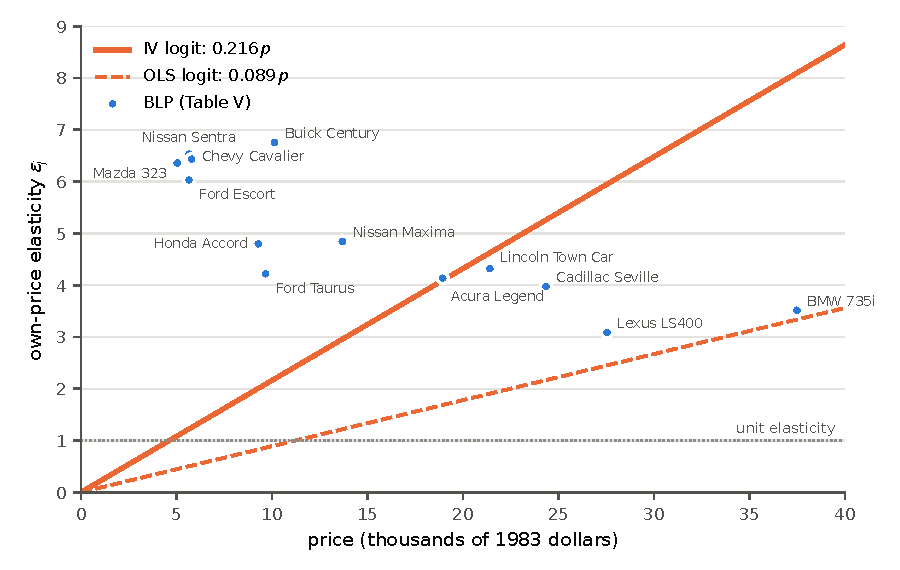
\includegraphics[width=0.86\textwidth]{figures/ch08/blp95_ownelas.pdf}
\caption{Own-price elasticities of thirteen 1990 models against price. Points are BLP's estimates
(their Table V). The rays are the logit elasticities $\alpha p$ implied by the IV and OLS logit price
coefficients of their Table III, ignoring the factor $1-s_j\approx1$. The dotted line marks unit
elasticity. Redrawn from \citet{BerryLevinsohnPakes1995}, Tables III and V.}
\label{fig:08-blp-ownelas}
\end{figure}

The price sensitivity of the marginal buyers can be read off the own semi-elasticities. Combining
\eqref{eq:08-blp-dsown} and \eqref{eq:08-blp-semi},
\begin{equation*}
-\frac{e_{jj}}{100}=\frac{1}{s_j}\int\frac{\alpha}{y_i-p_j}\,s_{ij}(1-s_{ij})\,\dd F(\nu_i)
\approx\E\Big[\frac{\alpha}{y_i-p_j}\,\Big|\,i\text{ buys }j\Big],
\end{equation*}
where the approximation uses $s_{ij}\ll1$. The semi-elasticities in \cref{tab:08-blp-semi} below give
$-\frac{e_{jj}}{100}=1.26$ for the Mazda 323, 0.52 for the Accord and 0.094 for the BMW 735i. Dividing
$\alpha=43.501$ by these numbers gives the harmonic mean of residual income $y_i-p_j$ among buyers. It is
about \$35,000 for the Mazda, \$84,000 for the Accord and \$464,000 for the BMW, in 1983 dollars (our
calculation). The specification can make luxury-car demand inelastic enough only by placing its buyers
far in the upper tail of the lognormal income distribution. This is one motivation for adding data on
buyers' incomes, as \citet{BerryLevinsohnPakes2004} and \citet{Petrin2002} later did
(\cref{sec:08-micro,sec:08-blp04}).

\casehead{Cross-price semi-elasticities}
BLP's Table VI reports own- and cross-price semi-elasticities for the same thirteen models.
\Cref{fig:08-blp-semielas} displays the full matrix, and \cref{tab:08-blp-semi} reproduces two diagonal
blocks. Entry $(i,j)$ is the percentage change in the share of row car $i$ when the price of column car
$j$ rises by \$1,000.

\begin{figure}[htbp]
\centering
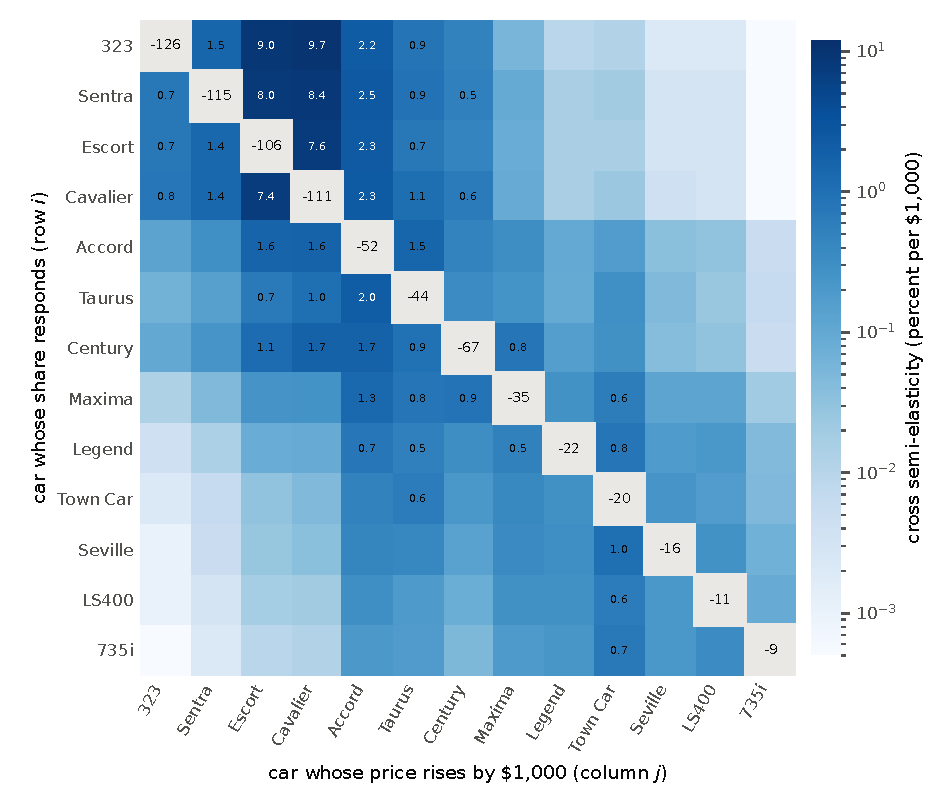
\includegraphics[width=0.9\textwidth]{figures/ch08/blp95_semielas.pdf}
\caption{Own- and cross-price semi-elasticities for thirteen 1990 models. Cell $(i,j)$ is the
percentage change in the share of row car $i$ for a \$1,000 increase in the price of column car $j$.
Off-diagonal cells are shaded on a log scale, and entries of at least 0.5 are printed. Diagonal cells
(gray) print the own semi-elasticity, which is negative. Entries printed as 0.000 in the source are
shaded at the bottom of the scale. Redrawn from \citet{BerryLevinsohnPakes1995}, Table VI.}
\label{fig:08-blp-semielas}
\end{figure}

\begin{table}[htbp]
\centering
\caption{Own- and cross-price semi-elasticities, two blocks of BLP (1995) Table VI}
\label{tab:08-blp-semi}
\small
\begin{tabular}{@{}lrrrr@{}}
\toprule
\multicolumn{5}{@{}l}{\emph{Panel A: small cars}}\\
Share of $\downarrow$ / price of $\rightarrow$ & Mazda 323 & Sentra & Escort & Cavalier \\
\midrule
Mazda 323 & $-125.933$ & 1.518 & 8.954 & 9.680 \\
Sentra    & 0.705 & $-115.319$ & 8.024 & 8.435 \\
Escort    & 0.713 & 1.375 & $-106.497$ & 7.570 \\
Cavalier  & 0.754 & 1.414 & 7.406 & $-110.972$ \\
\midrule
\multicolumn{5}{@{}l}{\emph{Panel B: luxury cars}}\\
Share of $\downarrow$ / price of $\rightarrow$ & Town Car & Seville & LS400 & BMW 735i \\
\midrule
Town Car  & $-20.175$ & 0.226 & 0.168 & 0.048 \\
Seville   & 1.011 & $-16.313$ & 0.263 & 0.068 \\
LS400     & 0.606 & 0.212 & $-11.199$ & 0.086 \\
BMW 735i  & 0.685 & 0.215 & 0.336 & $-9.376$ \\
\midrule
\multicolumn{5}{@{}l}{\emph{Panel C: small-car shares, luxury-car prices}}\\
Share of $\downarrow$ / price of $\rightarrow$ & Town Car & Seville & LS400 & BMW 735i \\
\midrule
Mazda 323 & 0.012 & 0.002 & 0.002 & 0.000 \\
Cavalier  & 0.023 & 0.004 & 0.003 & 0.000 \\
\bottomrule
\end{tabular}

\smallskip
\begin{minipage}{0.86\linewidth}
\footnotesize
Notes: Source: \citet{BerryLevinsohnPakes1995}, Table VI (p.~880), CRTS estimates. Entry
$(i,j)$ is $e_{ij}=\frac{100}{s_i}\frac{\partial s_i}{\partial p_j}$, the percentage change in the
share of row car $i$ for a \$1,000 increase in the price of column car $j$. The full $13\times13$ matrix
is shown in \cref{fig:08-blp-semielas}.
\end{minipage}
\end{table}

Three features stand out. First, own semi-elasticities fall sharply with price, from $-125.9$ for the
Mazda 323 to $-9.4$ for the BMW 735i. Multiplying each by $-\frac{p_j}{100}$ reproduces every own-price
elasticity in \cref{tab:08-blp-attr} to three decimals (our check). Under the IV logit every diagonal
entry would be about $-100\times0.216=-21.6$.

Second, cross effects are large among similar cars and close to zero across segments. A \$1,000 rise in
the Mazda 323's price raises the Sentra's share by 0.705 percent but leaves the Town Car, Seville, Lexus
and BMW almost unaffected. Under the logit the off-diagonal entries of a column would all equal
$100\,\alpha s_j$, whatever the row car. In BLP's matrix the largest cross entry in the Escort column is
about 1,000 times the smallest (8.954 against 0.009).

Third, the closest substitutes are intuitive. Measured down each column, the Lexus is the closest
substitute for the BMW 735i, the Cadillac Seville for the Lincoln Town Car, and the Accord for the Taurus
(p.~881). The effects of a \$1,000 increase are smaller for expensive cars because \$1,000 is a smaller
fraction of their price. Converting to elasticities removes this scale effect. For example, the
elasticity of the Seville's share with respect to the Town Car's price is
$1.011\times\frac{21.412}{100}\approx0.22$.

\casehead{Substitution to the outside good}
BLP measure how much of the demand a car loses goes to the outside good. The statistic is
\begin{equation*}
D_{j0}=100\times\frac{\frac{\partial s_0}{\partial p_j}}{\big|\frac{\partial s_j}{\partial p_j}\big|},
\end{equation*}
the number of consumers who switch from $j$ to no car, as a percentage of all who leave $j$ after a small
price rise. This is the diversion ratio to the outside good. Under the logit,
$\frac{\partial s_0}{\partial p_j}=\alpha s_0s_j$ and
$\big|\frac{\partial s_j}{\partial p_j}\big|=\alpha s_j(1-s_j)$, so
$D_{j0}=100\times\frac{s_0}{1-s_j}$. Under BLP, \cref{prop:08-diversion} gives
\begin{equation*}
\frac{D_{j0}}{100}=\int\varpi_{ij}\,\frac{s_{i0}}{1-s_{ij}}\,\dd F(\nu_i),\qquad
\varpi_{ij}=\frac{\frac{\alpha}{y_i-p_j}\,s_{ij}(1-s_{ij})}
{\int\frac{\alpha}{y_l-p_j}\,s_{lj}(1-s_{lj})\,\dd F(\nu_l)},
\end{equation*}
a weighted average of individual diversions with weights concentrated on the price-sensitive marginal
buyers of $j$.

\begin{table}[htbp]
\centering
\caption{Substitution to the outside good after a price increase (BLP 1995, Table VII)}
\label{tab:08-blp-outside}
\small
\begin{tabular}{@{}lrr@{}}
\toprule
Model & Logit & BLP \\
\midrule
Mazda 323 & 90.870 & 27.123 \\
Nissan Sentra & 90.843 & 26.133 \\
Ford Escort & 90.592 & 27.996 \\
Chevy Cavalier & 90.585 & 26.389 \\
Honda Accord & 90.458 & 21.839 \\
Ford Taurus & 90.566 & 25.214 \\
Buick Century & 90.777 & 25.402 \\
Nissan Maxima & 90.790 & 21.738 \\
Acura Legend & 90.838 & 20.786 \\
Lincoln Town Car & 90.739 & 20.309 \\
Cadillac Seville & 90.860 & 16.734 \\
Lexus LS400 & 90.851 & 10.090 \\
BMW 735i & 90.883 & 10.101 \\
\bottomrule
\end{tabular}

\smallskip
\begin{minipage}{0.62\linewidth}
\footnotesize
Notes: Source: \citet{BerryLevinsohnPakes1995}, Table VII (p.~881). Entries are
$D_{j0}=100\times\frac{\partial s_0}{\partial p_j}\Big(\Big|\frac{\partial s_j}{\partial p_j}\Big|\Big)^{-1}$,
the percentage of consumers who leave car $j$ after a small price increase and choose the outside good.
\end{minipage}
\end{table}

\begin{figure}[htbp]
\centering
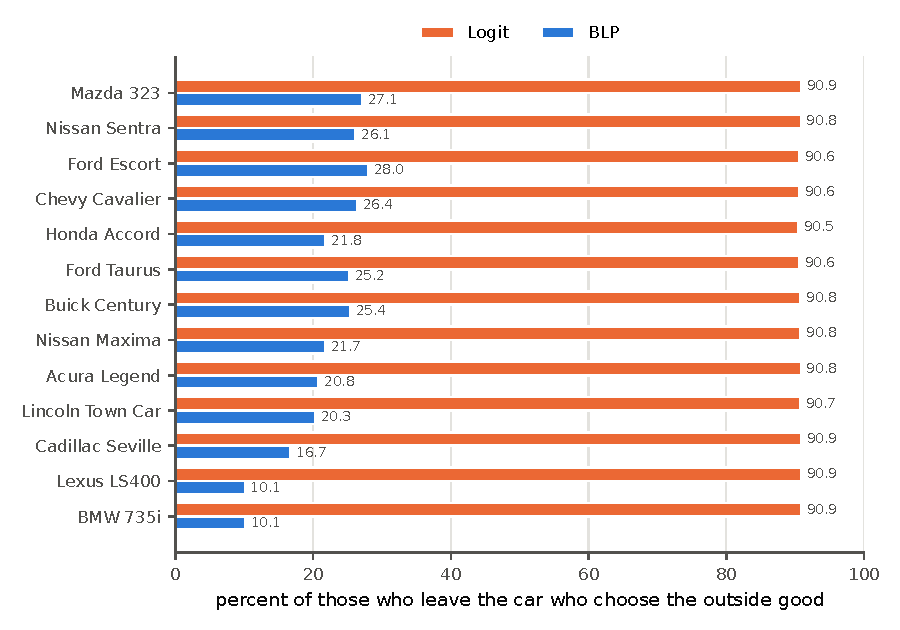
\includegraphics[width=0.82\textwidth]{figures/ch08/blp95_outside.pdf}
\caption{Diversion to the outside good after a small price increase, logit against BLP. Redrawn from
\citet{BerryLevinsohnPakes1995}, Table VII.}
\label{fig:08-blp-outside}
\end{figure}

\Cref{tab:08-blp-outside} and \cref{fig:08-blp-outside} report the results. Under the logit about 90
percent of those who leave any model choose no car, which is $\frac{s_0}{1-s_j}\approx s_0$. The logit
column ranges from 90.458 to 90.883. Since $\frac{s_0}{1-s_j} > s_0$, this puts $s_0$ just below 0.905.
The entries fall slightly with sales, which $\frac{s_0}{1-s_j}$ does not allow, so the printed values
match the formula only approximately. Under
BLP's estimates the diversion ranges from 28.0 percent (Escort) to 10.1 percent (Lexus and BMW). It is
lower for expensive cars. Buyers of luxury cars are rich and like cars, so for them $s_{i0}$ is small and
they move to other luxury cars. Buyers of cheap cars are closer to the margin of not buying. BLP still
find their numbers ``a bit large'' and see this as a sign that the treatment of the outside good needs
improvement (pp.~881--882). The outside good includes keeping an old car, and a dynamic model with a
used-car market would treat it more realistically (Section 8.2 of the paper).

\subsection{Results IV: markups and profits}\label{sec:08-blp95-markups}

Markups combine the demand and cost estimates. \Cref{tab:08-blp-markups} reproduces BLP's Table VIII
and adds four columns that we compute from it and from Table V.

\begin{table}[htbp]
\centering
\caption{Markups and variable profits for 1990 models, CRTS estimates (BLP 1995, Table VIII, with
derived columns)}
\label{tab:08-blp-markups}
\footnotesize
\setlength{\tabcolsep}{4pt}
\begin{tabular}{@{}llrrrrrrr@{}}
\toprule
 & & \multicolumn{3}{c}{BLP Table VIII} & \multicolumn{4}{c}{Derived (our calculation)} \\
\cmidrule(lr){3-5}\cmidrule(l){6-9}
Model & Firm & Price & $p-mc$ & $q(p-mc)$ & $\frac{p-mc}{p}$ & $\frac{1}{\varepsilon_j}$ & Gap
 & Sales \\
\midrule
Mazda 323        & Mazda  & 5,049  & 801    & 18,407  & 0.159 & 0.157 & 0.001 & 22,980 \\
Nissan Sentra    & Nissan & 5,661  & 880    & 43,554  & 0.155 & 0.153 & 0.002 & 49,493 \\
Ford Escort      & Ford   & 5,663  & 1,077  & 311,068 & 0.190 & 0.166 & 0.024 & 288,828 \\
Chevy Cavalier   & GM     & 5,797  & 1,302  & 384,263 & 0.225 & 0.155 & 0.069 & 295,133 \\
Honda Accord     & Honda  & 9,292  & 1,992  & 830,842 & 0.214 & 0.208 & 0.006 & 417,089 \\
Ford Taurus      & Ford   & 9,671  & 2,577  & 807,212 & 0.266 & 0.237 & 0.029 & 313,237 \\
Buick Century    & GM     & 10,138 & 2,420  & 271,446 & 0.239 & 0.148 & 0.091 & 112,168 \\
Nissan Maxima    & Nissan & 13,695 & 2,881  & 288,291 & 0.210 & 0.206 & 0.004 & 100,066 \\
Acura Legend     & Honda  & 18,944 & 4,671  & 250,695 & 0.247 & 0.242 & 0.005 & 53,671 \\
Lincoln Town Car & Ford   & 21,412 & 5,596  & 832,082 & 0.261 & 0.231 & 0.030 & 148,692 \\
Cadillac Seville & GM     & 24,353 & 7,500  & 249,195 & 0.308 & 0.252 & 0.056 & 33,226 \\
Lexus LS400      & Toyota & 27,544 & 9,030  & 371,123 & 0.328 & 0.324 & 0.004 & 41,099 \\
BMW 735i         & BMW    & 37,490 & 10,975 & 114,802 & 0.293 & 0.284 & 0.008 & 10,460 \\
\bottomrule
\end{tabular}

\smallskip
\begin{minipage}{0.97\linewidth}
\footnotesize
Notes: Columns 3 to 5 are from \citet{BerryLevinsohnPakes1995}, Table VIII (p.~882), whose
caption refers to ``Table 6 (CRTS)'' estimates, meaning those of Table IV. Price and markup are in 1983
dollars, and variable profits in thousands of 1983 dollars. ``Firm'' is the parent company. The last
four columns are our calculations: the Lerner index, the inverse own-price elasticity from Table V, the
gap between them, and implied unit sales $\frac{q(p-mc)}{p-mc}$.
\end{minipage}
\end{table}

\casehead{Levels and pattern}
In 1990 the average markup is \$3,753 and the average ratio of markup to price is 0.239 (p.~882). The
lowest markups are those of the Mazda 323 (\$801), Sentra (\$880) and Escort (\$1,077). The Lexus and
BMW have markups of \$9,030 and \$10,975. Markups rise almost monotonically with price, and the Lerner
index rises from about 0.16 to about 0.3. \Cref{fig:08-blp-markup} contrasts this pattern with the IV
logit, whose markups all lie in a band between \$4,630 and \$4,805. BLP note that the average level of
markups is similar in the two models even though the pattern differs (footnote 31).

\begin{figure}[htbp]
\centering
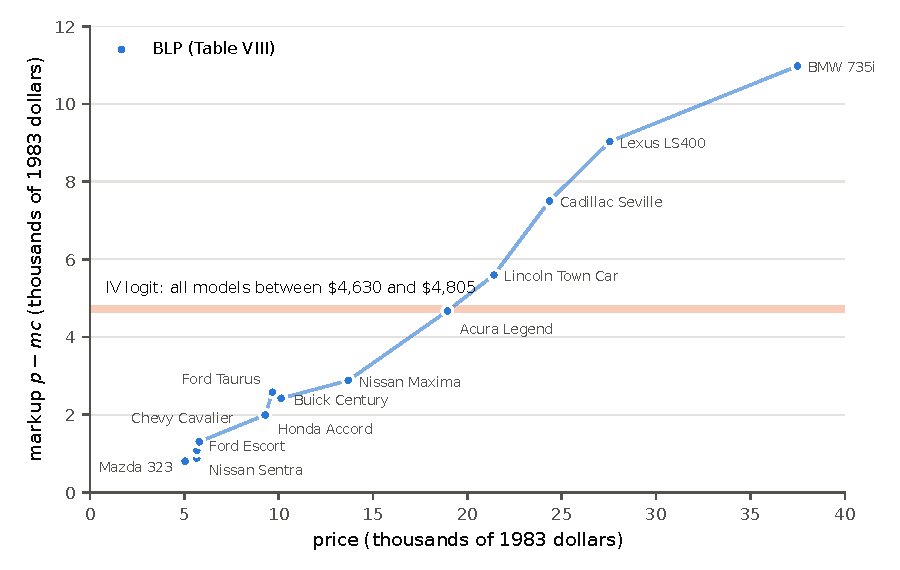
\includegraphics[width=0.86\textwidth]{figures/ch08/blp95_markup.pdf}
\caption{Price-cost markups of thirteen 1990 models against price. Points are BLP's estimates (their
Table VIII). The shaded band is the range of markups implied by the IV logit for all 1990 models
(\$4,630 to \$4,805, p.~874). Redrawn from \citet{BerryLevinsohnPakes1995}.}
\label{fig:08-blp-markup}
\end{figure}

\casehead{Profits}
Large markups need not mean large profits, because some high-markup cars sell few units. BLP single out
the Honda Accord and the Ford Taurus as the most profitable models in their table, by a factor of two
relative to most others. Both were regarded as essential to their firms' finances
(p.~882).\footnote{In the printed Table VIII the Lincoln Town Car's variable profit (\$832,082 thousand)
is as large as the Accord's (\$830,842 thousand) and the Taurus's (\$807,212 thousand). The text's
statement fits the other ten models.} Dividing variable profits by markups recovers unit sales, which
range from 10,460 BMW 735i's to 417,089 Accords.

\casehead{Multi-product pricing in the markups}
The derived columns of \cref{tab:08-blp-markups} reveal the role of multi-product ownership. The
following decomposition holds in any Bertrand-Nash equilibrium.

\begin{proposition}[Multi-product Lerner index]\label{prop:08-blp-lerner}
Let $D_{jr}=\frac{\partial s_r}{\partial p_j}\Big(\Big|\frac{\partial s_j}{\partial p_j}\Big|\Big)^{-1}$
be the diversion ratio from $j$ to $r$. At an interior Bertrand-Nash equilibrium, every product $j$ of firm $f$ satisfies
\begin{equation*}
\frac{p_j-mc_j}{p_j}=\frac{1}{\varepsilon_j}
 +\sum_{r\in\mathcal{J}_f,\,r\neq j}D_{jr}\,\frac{p_r-mc_r}{p_j}.
\end{equation*}
If the products are substitutes and markups are positive, the second term is nonnegative, so
$\varepsilon_j>1$ whenever the Lerner index is below one.
\end{proposition}

\begin{proof}
Move the own-product term of \eqref{eq:08-foc} to the left:
\begin{equation*}
(p_j-mc_j)\Big(-\frac{\partial s_j}{\partial p_j}\Big)=s_j
 +\sum_{r\in\mathcal{J}_f,\,r\neq j}(p_r-mc_r)\frac{\partial s_r}{\partial p_j}.
\end{equation*}
Divide both sides by $p_j\big|\frac{\partial s_j}{\partial p_j}\big|$. The first term on the right
becomes $\frac{s_j}{p_j}\Big(\Big|\frac{\partial s_j}{\partial p_j}\Big|\Big)^{-1}=\frac{1}{\varepsilon_j}$,
and each term of the
sum becomes $D_{jr}\frac{p_r-mc_r}{p_j}$. With substitutes $D_{jr}\geq0$ and positive markups, so the
sum is nonnegative. Then $\frac{1}{\varepsilon_j}\leq\frac{p_j-mc_j}{p_j}<1$ gives
$\varepsilon_j>1$.
\end{proof}

The gap between the Lerner index and $\frac{1}{\varepsilon_j}$ measures the margins a firm recaptures
on its other products. For the products of Mazda, Nissan, Honda, Toyota and BMW the gap is at most
0.008. Their 1990 portfolios contained few close substitutes for these models. For Ford's Escort, Taurus
and Town Car the gap is 0.024 to 0.030. For GM's Cavalier, Century and Seville it is 0.056 to 0.091.
GM's many divisions sell close substitutes for each of its models, so a price rise on the Century
diverts many buyers to other GM cars. This portfolio effect, invisible in the logit except through
$S_f$, is the mechanism that \citet{Nevo2001} later used to separate multi-product pricing from collusion
(\cref{sec:08-nevo01}).

\subsection{Robustness}\label{sec:08-blp95-robust}

The choice of characteristics in utility and cost is ad hoc, and computation limits the number of
random coefficients. BLP report how markups change across six alternative specifications. They choose
markups as the summary because markups combine demand and cost information and are easy to interpret.
\Cref{tab:08-blp-robust} reproduces their Table IX.

\begin{table}[htbp]
\centering
\caption{Markups under alternative specifications, 1990 models, dollars (BLP 1995, Table IX)}
\label{tab:08-blp-robust}
\footnotesize
\setlength{\tabcolsep}{4pt}
\begin{tabular}{@{}lrrrrrrr@{}}
\toprule
 & (1) & (2) & (3) & (4) & (5) & (6) & (7) \\
 & \makecell{Base\\(Table VIII)} & \makecell{$\ln q$\\in cost} & \makecell{AT\\for Air}
 & \makecell{Weight, HP\\for HPWT} & \makecell{Cost\\interactions} & \makecell{Regions,\\reliability}
 & \makecell{Weight,\\interactions} \\
\midrule
Mazda 323        & 801    & 1,616  & 1,012 & 1,073 & 828    & 1,125  & 1,389 \\
Nissan Sentra    & 880    & 1,769  & 1,153 & 1,271 & 912    & 1,308  & 1,487 \\
Ford Escort      & 1,077  & 2,043  & 1,326 & 1,470 & 1,111  & 2,094  & 1,690 \\
Chevy Cavalier   & 1,302  & 2,490  & 1,729 & 1,655 & 1,329  & 2,593  & 2,020 \\
Honda Accord     & 1,992  & 3,059  & 2,629 & 2,703 & 2,059  & 3,839  & 2,327 \\
Ford Taurus      & 2,577  & 3,721  & 2,528 & 3,344 & 2,585  & 4,094  & 2,898 \\
Buick Century    & 2,420  & 4,162  & 3,161 & 2,939 & 2,405  & 4,030  & 3,321 \\
Nissan Maxima    & 2,881  & 4,674  & 4,565 & 2,085 & 2,911  & 6,941  & 3,513 \\
Acura Legend     & 4,671  & 7,105  & 6,563 & 3,059 & 4,661  & 8,305  & 5,081 \\
Lincoln Town Car & 5,596  & 8,029  & 6,778 & 4,765 & 5,508  & 7,114  & 6,518 \\
Cadillac Seville & 7,500  & 10,733 & 8,635 & 4,863 & 7,439  & 9,182  & 8,015 \\
Lexus LS400      & 9,030  & 10,510 & 8,411 & 4,791 & 8,585  & 10,925 & 7,398 \\
BMW 735i         & 10,975 & 13,646 & 9,122 & 7,605 & 10,713 & 12,153 & 12,202 \\
\midrule
Demand variables significant & 5 of 5 & 4 of 5 & 4 of 5 & 6 of 6 & 4 of 5 & 8 of 8 & 4 of 6 \\
\bottomrule
\end{tabular}

\smallskip
\begin{minipage}{0.97\linewidth}
\footnotesize
Notes: Source: \citet{BerryLevinsohnPakes1995}, Table IX (p.~883). Price minus marginal cost in
1983 dollars. (2) adds $\ln q$ to the cost function (last columns of Table IV). (3) replaces Air with a
dummy for standard automatic transmission. (4) replaces HPWT with horsepower and weight entered
separately. (5) adds interactions of the continuous characteristics to the cost function. (6) replaces
the constant in utility with U.S., Japan and Europe dummies and adds the reliability rating. (7) adds
weight and cost-side interactions. The last row counts demand variables whose mean or standard
deviation is significant at the 95 percent level.
\end{minipage}
\end{table}

The pattern of markups survives every specification. In each column markups rise broadly with price, with a few
reversals, and the correlation of each column with the base column is between 0.945 and 0.9997 (our calculation). Levels
move more. Across the seven columns a car's highest markup is between 1.6 and 3.3 times its lowest.

The individual columns have specific explanations (pp.~883--885). Adding $\ln q$ in column (2) raises
every markup, and it gives the highest markups of all the alternatives, yet even these are not
extraordinarily high. As shown above, its markups over average variable cost are implausible. Using
automatic transmission as the luxury proxy in column (3) raises markups slightly for cheap cars and lowers
them slightly for expensive ones. Entering horsepower and weight separately in column (4) changes markups
the most. It gives implausibly low markups for expensive cars, possibly because cost is not linear in
horsepower and weight. Cost interactions in column (5) leave markups within a few percent of the base,
although most interaction terms are significant. Region dummies with reliability in column (6) raise
markups for several mid-priced models from different regions, for reasons BLP could not identify.
Reliability is included there because region dummies may be correlated with reliability, which would
otherwise sit in $\xi$ and invalidate the instruments. Column (7) adds weight, which has an
insignificant cost coefficient and a significant demand mean, and leaves markups close to the base.

\subsection{Interpretation}\label{sec:08-blp95-interp}

BLP read Tables IV to VIII as evidence that flexible utility gives a more realistic picture of
equilibrium in the industry. Three lessons stand out.

First, instrumenting for price matters even in the logit. It more than doubles the price coefficient
and removes almost all inelastic demands (\cref{tab:08-blp-logit}). Second, random coefficients and
income effects change the economics, beyond the econometrics. Own elasticities fall with price,
substitution runs between similar cars, and diversion to the outside good falls from about 90 percent to
10 to 28 percent. Each of these patterns is impossible in the logit. Third, the implied markups are
plausible in level and pattern. They are consistent with standard multi-product pricing, in which GM's
broad portfolio raises its margins above the inverse elasticity.

The results have clear implications for counterfactuals. A merger simulation built on the logit would
predict uniform markups and diversion mostly to the outside good. It would therefore understate the
price effects of merging close substitutes (\cref{ch:mergers}). A tariff analysis would mispredict which
domestic cars gain from higher import prices. A welfare calculation for a new model would depend on how
much demand it takes from similar cars.

\subsection{Limitations and critiques}\label{sec:08-blp95-critique}

\casehead{Data}
Prices are list prices of base models, so discounts and options are missing. Fleet sales are ignored.
Output is poorly measured for imported models, which limits the cost function. Market size is the number
of households, and every household is assumed to consider buying one new car each year.

\casehead{Exogenous characteristics}
The moment condition \eqref{eq:08-blp-moments} treats observed characteristics as mean independent of
$\xi$ and $\omega$. Firms choose characteristics, and they may choose them knowing $\xi$, so the
instruments may be invalid. BLP raise this concern themselves and sketch a Markov alternative
(\cref{sec:08-blp95-estimation}). They also identify obtaining consistent estimates when observed and
unobserved characteristics are correlated as the easier part of the dynamic problem. Endogenizing the
choice of characteristics is the harder part (Section 8.2 of the paper).

\casehead{Statics and the outside good}
Cars are durable. A household's outside option is often its current car, and its timing of purchases
responds to prices and expectations. A static model with an undifferentiated outside good cannot capture
these choices, which may explain why diversion to the outside good still looks large.

\casehead{Conditional counterfactuals}
Policy analysis with the model holds characteristics and the product set fixed. \citet{PakesBerryLevinsohn1993}
used the estimates to predict average MPG after the 1973 gasoline price shock. The model predicted 1974
and 1975 almost exactly, when characteristics changed little. From 1976 on, new small fuel-efficient
models appeared and the predictions became markedly worse (pp.~885--886).

\casehead{Functional form and the supply side}
All heterogeneity in price sensitivity comes from income through $\alpha\ln(y_i-p_j)$, with one income
dispersion parameter for all years. Our harmonic-mean calculation shows how far into the income tail the
model must place luxury-car buyers. The random coefficients are independent normals. Conduct is assumed
to be Bertrand-Nash and is not tested. The constant-returns cost function produces a negative MPG
coefficient, and the alternative with $\ln q$ implies implausible returns to scale.

\casehead{Aggregate data only}
BLP use no data that link households to the cars they buy. Their own conclusion points to consumer
surveys and to plant-level cost data from the Census Longitudinal Research Database (Section 8.2 of the paper).
\citet{BerryLevinsohnPakes2004} and \citet{Petrin2002} later added consumer-level moments for cars
(\cref{sec:08-micro,sec:08-blp04}), and \citet{Goldberg1995} estimated car demand from household data
(\cref{sec:08-goldberg}).

\casehead{Numerical and instrument sensitivity}
Later work re-examined the estimator. \citet[p.~35]{KnittelMetaxoglou2014} used BLP's automobile data and the
synthetic cereal data of \citet{Nevo2000a}. They found that BLP-type estimates and their implications can vary
with the optimization algorithm and starting values.
\citet{DubeFoxSu2012} showed that a loose tolerance in the contraction can produce false convergence
(\cref{sec:08-inversion,sec:08-practice}). \citet[Section~3]{Armstrong2016} showed that the characteristics-based
instruments can lose their power in markets with many products. Equilibrium markups then vary little.
\citet{ReynaertVerboven2014} and \citet[Section~5]{ConlonGortmaker2020} found in Monte Carlo experiments that
approximations to the optimal instruments improve precision.
These critiques concern implementation, and they leave the framework itself intact.

\subsection{Contribution}\label{sec:08-blp95-contrib}

BLP's contribution is a complete template for empirical work on differentiated products with market-level
data. It combines five elements. Utility is defined over characteristics, with random coefficients and
demographic information from outside the sample. Shares are aggregated by simulation. Mean utilities
are recovered by inverting the share equations with a contraction. A GMM estimator built on structural
errors handles price endogeneity, with instruments derived from oligopoly pricing and exchangeability.
A multi-product Nash pricing equation recovers marginal costs and markups without cost data.

The same template now underlies most empirical work on differentiated-products markets. Applications
include voluntary export restraints on Japanese cars \citep{BerryLevinsohnPakes1999}, mergers
\citep[\cref{ch:mergers}]{Nevo2000b}, the welfare gains from new goods
\citep[\cref{ch:newgoods}]{Petrin2002}, and airline hubs \citep[\cref{ch:airlines}]{BerryCarnallSpiller2006}.
\citet{Nevo2000a} wrote the guide that made the method accessible, and we turn to it next.

\section{Case study: Nevo (2000a), the practitioner's guide and its application}\label{sec:08-nevo00}

\citet{Nevo2000a} is a guide to the random coefficients logit for researchers who have not used it. It
explains the model, the algorithm and the instruments with the stated aim of lowering the barriers to
entry and increasing trust in the method among outsiders (p.~514). It ends with an application to a
synthetic data set, and Nevo posted the data and his Matlab code. The model and algorithm of
\cref{sec:08-model,sec:08-substitution,sec:08-simulation,sec:08-inversion,sec:08-gmm,sec:08-instruments}
follow the guide's equations closely. This section covers the rest: the guide's framing, its
specification choices and their implications, its practical advice, the application in full, and its
list of extensions.

\subsection{Purpose and framing}\label{sec:08-nevo00-purpose}

Nevo starts from two problems that make differentiated-products demand hard. The first is
dimensionality. A log-log demand system for 100 products has 100 equations, each with 100 prices, which
means at least 10,000 parameters (p.~514). Symmetry and adding up remove only part of these, and the
number remains too large to estimate. More flexible substitution patterns make the problem worse. The
second is heterogeneity. If all consumers were identical, markets would not show the variety of products
we observe. A representative consumer exists under Gorman-form preferences \citep{Gorman1959}, but those
assumptions are strong and often empirically false.

The logit model solves the dimensionality problem by projecting products onto a space of
characteristics. The number of parameters then depends on the number of characteristics and not on the
square of the number of products. The cost is the logit's treatment of heterogeneity, which makes
substitution depend on market shares and not on how similar products are. Random coefficients keep the
projection and model heterogeneity explicitly. Nevo lists three advantages of the BLP method over earlier
estimates of such models (p.~515). It needs only market-level price and quantity data, it deals with the
endogeneity of prices, and it produces more realistic elasticities.

\subsection{Specification choices and their implications}\label{sec:08-nevo00-spec}

\casehead{The guide's model}
The guide's model is the one of \cref{sec:08-linear}. Indirect utility is \eqref{eq:08-nevo-utility} (his
eq.~1), and tastes depend on demographics and unobserved characteristics as in \eqref{eq:08-tastes} (his
eq.~2). The unobserved tastes $\nu_i$ come from a parametric distribution, usually standard normal, and the
demographics $D_i$ from an empirical distribution such as CPS draws. The outside good is normalized as in \cref{sec:08-normalization}. Combining the
two equations gives the decomposition \eqref{eq:08-decomposition} (his eq.~3), and shares integrate over
$(D,\nu,\epsilon)$ with the factorization \eqref{eq:08-share-bayes} (his eq.~4).

\casehead{Assumptions and their implications}
Nevo spells out three assumptions implicit in \eqref{eq:08-nevo-utility} and then discusses how
\eqref{eq:08-tastes} models heterogeneity (pp.~517--520).
\begin{enumerate}
\item \emph{No wealth effects.} The form $\alpha_i(y_i-p_{jt})$ comes from quasilinear utility. This is
  reasonable for ready-to-eat cereal and unreasonable for cars. BLP's $\ln(y_i-p_j)$ is one alternative,
  and a flexible function $f(y_i-p_{jt})$ is another, as in \citet{Petrin2002}.
\item \emph{A common valuation of $\xi$.} Every consumer values the unobserved characteristic equally.
  Because the price coefficient varies, this is consistent with theories of vertical differentiation.
  \citet{DasOlleyPakes1994} model a distribution of valuations of $\xi$ instead.
\item \emph{Common prices and characteristics.} All consumers in a market face the same price. If they
  do not, a list or average price measures the relevant price with error. This is one more reason why
  price may be correlated with the error. The inversion method handles measurement error only if the
  mismeasured variable enters $\delta_{jt}$ alone (footnote 11, citing \citealp{Berry1994}).
\item \emph{Observed and unobserved heterogeneity.} Demographics bring outside information into the
  model and reduce reliance on parametric assumptions. Nevo's example of an unobserved characteristic is
  whether a household owns a dog, which matters for choosing a car but appears in no survey (p.~519). The
  linear form $\Pi D_i$ is restrictive, especially for the price coefficient.
\end{enumerate}

\casehead{Where correlation in utility comes from}
Nevo then explains why the logit fails and how to fix it (pp.~522--526), with the arguments and the cereal
examples that \cref{sec:08-logit-benchmark} reproduced. The cure is correlation in utility across brands, which
can enter through $\epsilon$ or through $\mu$.
Generalized extreme value models put it in $\epsilon$. The nested logit groups brands into exhaustive and
mutually exclusive nests fixed in advance. Within a nest, substitution is again proportional to shares,
and the model does nothing for own elasticities. \citet{Cardell1997} shows the distributional assumptions
under which a random coefficient on segment dummies reproduces the nested logit. With several layers of
segmentation the order of the nests matters. Grouping computers first by brand and then by technology
gives different substitution than the reverse order, even with the same groups (footnote 18). The
principles-of-differentiation GEV model of \citet{BresnahanSternTrajtenberg1997} avoids ordering the
nests. An unrestricted covariance matrix for $\epsilon$ reintroduces the dimensionality problem.

The random coefficients model puts the correlation in $\mu$. Products with similar characteristics are
correlated in utility, and consumers with similar demographics rank products similarly. The own-price
derivative averages individual price sensitivities with weights given by individual purchase
probabilities (\cref{prop:08-derivs}). If the buyers of Kellogg's Corn Flakes are price sensitive, its
own elasticity is high despite its low price (p.~526). Substitution is then driven by differences in
price sensitivity across the buyers of different products, and not by the functional form.

\subsection{Practical recommendations}\label{sec:08-nevo00-practice}

The guide's Section 3 turns from the model to practice. Most of its advice is now part of the chapter's
theory, and we list each item with the place where we develop it.

\casehead{Data and market size}
The data requirements and Nevo's four rules for choosing the market size are those of \cref{sec:08-data}
(p.~527). Nevo strongly recommends several markets with variation in relative prices or in the products
offered.

\casehead{Two roles of characteristics}
Characteristics explain mean utility $\delta$ and drive substitution through $\mu$, and Nevo recommends keeping
the two roles separate (pp.~527--528, \cref{sec:08-assumptions}). Substitution must come from characteristics,
which should therefore guide what the researcher collects.

\casehead{Identification}
Nevo's informal argument starts from an ideal experiment that randomizes prices across consumers
(pp.~528--530). Market data depart from it in two ways. Prices are set by firms that know $\xi$, which
instruments address. More subtly, a discrete choice model can be estimated from one market. Each market
is then an observation on the relative likelihood of buying $J$ bundles of attributes, one of which is
price. Identification improves with more markets that vary in product characteristics, choice sets and
demographic distributions. His three-product example (A and B similar, B and C with equal shares) appears in
\cref{sec:08-illustration,sec:08-iv-roles}.

\casehead{The estimator}
The guide argues against matching shares by nonlinear least squares (his eq.~7) and builds the GMM residual
from the inverted mean utilities (his eqs.~8 to 13). It notes that the logit and nested logit reduce to
two-stage least squares. \Cref{sec:08-gmm} develops all three points.

\casehead{Instruments}
Nevo reviews cost shifters, characteristics-based instruments and Hausman instruments with their caveats
(pp.~534--536), as in \cref{sec:08-iv-families}. His footnote 23 makes the characteristics-based instruments
concrete. Suppose there are two characteristics (horsepower and size) and two firms with three products each.
The instruments for a product are then its two characteristics, their sums over the firm's other two products,
and their sums over the rival's three products, six in all. Nevo stresses that validity must be argued case by
case.

\casehead{Brand dummies and minimum distance}
Nevo believes brand fixed effects should be used whenever possible (p.~536). \Cref{sec:08-brand-fe} develops his
argument, his answers to the two objections and the minimum-distance estimator \eqref{eq:08-md} of the taste
parameters (pp.~537--538). The assumption $\E[\xi_b\mid \bm{X}_b]=0$ is used only to recover $\beta$. A
researcher unwilling to make it can still recover price sensitivity from the other instruments (footnote 24).

\subsection{The application}\label{sec:08-nevo00-app}

\casehead{Data}
The data contain prices and quantities for 24 brands of a differentiated product in 47 cities over 2
quarters (p.~538). A market is a city-quarter, so there are 94 markets and $24\times94=2{,}256$
observations. Every brand is sold in every market, so choice sets do not vary. The data were generated
from the demand model of Section 2 and a multi-product Bertrand pricing model (footnote 25). The marginal
costs and parameters were motivated by the cereal estimates of \citet{Nevo2000b}. Nevo warns that the data
are not real and should not be used for analysis. Their purpose is to teach the method.

Products have two characteristics. \emph{Sugar} measures sugar content, and \emph{Mushy} equals one if
the cereal gets soggy in milk. Demographics are drawn from the CPS: the log of income (\emph{Income}), its
square (\emph{IncomeSq}), \emph{Age}, and \emph{Child}, a dummy for being under sixteen. The unobserved
$\nu_i$ are standard normal, and each market uses $n_s=20$ simulated individuals. All specifications
include brand and time dummies. Section~4 does not describe the instruments used in the application.

\casehead{Specification}
The pattern of entries in Nevo's Table I reveals the estimated specification. Write $b_i^p=-\alpha_i$
for the price coefficient, which is what the table reports. Then
\begin{align*}
b_i^{p}&=b^{p}+\pi_{p,1}\mathit{Income}_i+\pi_{p,2}\mathit{IncomeSq}_i+\pi_{p,3}\mathit{Child}_i
 +\sigma_p\nu_{ip},\\
\beta_i^{k}&=\beta^{k}+\pi_{k,1}\mathit{Income}_i+\pi_{k,2}\mathit{Age}_i+\sigma_k\nu_{ik},
 \qquad k\in\{\text{Constant},\text{Sugar},\text{Mushy}\}.
\end{align*}
The nonlinear parameters are four standard deviations and nine demographic interactions, so $\theta_2$
has 13 elements. The means of the constant, Sugar and Mushy are absorbed by the brand dummies and
recovered by the minimum-distance step \eqref{eq:08-md} with 24 brand effects.

\begin{table}[htbp]
\centering
\caption{Results from the full model, synthetic cereal data (Nevo 2000a, Table I)}
\label{tab:08-nevo00-results}
\small
\begin{tabular}{@{}lrrrrrr@{}}
\toprule
 & Means & Std.\ dev. & \multicolumn{4}{c}{Interactions with demographic variables} \\
\cmidrule(l){4-7}
Variable & $\beta$ & $\sigma$ & Income & IncomeSq & Age & Child \\
\midrule
Price    & $-32.433$ & 1.848 & 16.598 & $-0.659$ & & 11.625 \\
         & (7.743) & (1.075) & (172.334) & (8.955) & & (5.207) \\
Constant & $-1.841^{a}$ & 0.377 & 3.089 & & 1.186 & \\
         & (0.258) & (0.129) & (1.213) & & (1.016) & \\
Sugar    & $0.148^{a}$ & 0.004 & $-0.193$ & & 0.029 & \\
         & (0.258) & (0.012) & (0.005) & & (0.036) & \\
Mushy    & $0.788^{a}$ & 0.081 & 1.468 & & $-1.514$ & \\
         & (0.013) & (0.205) & (0.697) & & (1.103) & \\
\midrule
GMM objective & & & 14.9 & & & \\
(Degrees of freedom) & & & (7) & & & \\
\bottomrule
\end{tabular}

\smallskip
\begin{minipage}{0.9\linewidth}
\footnotesize
Notes: Source: \citet{Nevo2000a}, Table I (p.~539). Based on 2,256 observations. Except where
noted, parameters are GMM estimates. All regressions include brand and time dummy variables.
Asymptotically robust standard errors in parentheses. $^{a}$Estimates from the minimum-distance
procedure. Blank cells are interactions not included in the specification.
\end{minipage}
\end{table}

\casehead{Results}
\Cref{tab:08-nevo00-results} reproduces Nevo's Table I. The minimum-distance means say that the average
consumer gains utility from more sugar (0.148) and from sogginess (0.788). The standard deviations
capture unobserved heterogeneity. Nevo describes them as insignificant both economically and
statistically, and he expects them to stay statistically insignificant even with more efficient
estimation (footnote 26).\footnote{By the printed standard errors, the standard deviation on the
constant (0.377, with standard error 0.129) has a $t$ ratio near 2.9. The other three standard deviations
are insignificant.}

The demographic interactions have economically large point estimates, although most are imprecise. The
valuation of sogginess falls with age ($-1.514$). Nevo says it also falls with income, while the printed
income interaction is positive (1.468).\footnote{The text on p.~540 states that ``the marginal valuation
of sogginess decreases with age and income.'' The income interaction in Table I is $+1.468$ with standard
error 0.697. We report the table.} \Cref{fig:08-nevo00-dists}(a) shows the implied distribution of the
Mushy coefficient across consumers. Most consumers value sogginess positively, but about 31
percent prefer a crunchy cereal (p.~540). Sugar is valued less by richer consumers, and this interaction
is very precisely estimated ($-0.193$, standard error 0.005).

The mean price coefficient is $-32.433$. Children are less price sensitive. Their price coefficient is
higher by 11.625, which is 36 percent of the mean coefficient and 6.3 times the unobserved standard
deviation $\sigma_p=1.848$ (our calculation). Nevo also reports that above-average-income consumers are
less price sensitive. The income terms are very imprecise, with a standard error of 172.334 on the linear
term. \Cref{fig:08-nevo00-dists}(b) shows the distribution of individual price coefficients. It is not
normal, because it inherits the shape of the empirical distribution of demographics. Its mass lies
between about $-70$ and $-15$, so no consumer has a positive price coefficient, although a linear
specification allows one in principle (p.~540).

\begin{figure}[htbp]
\centering
\begin{subfigure}[t]{0.72\textwidth}
\centering
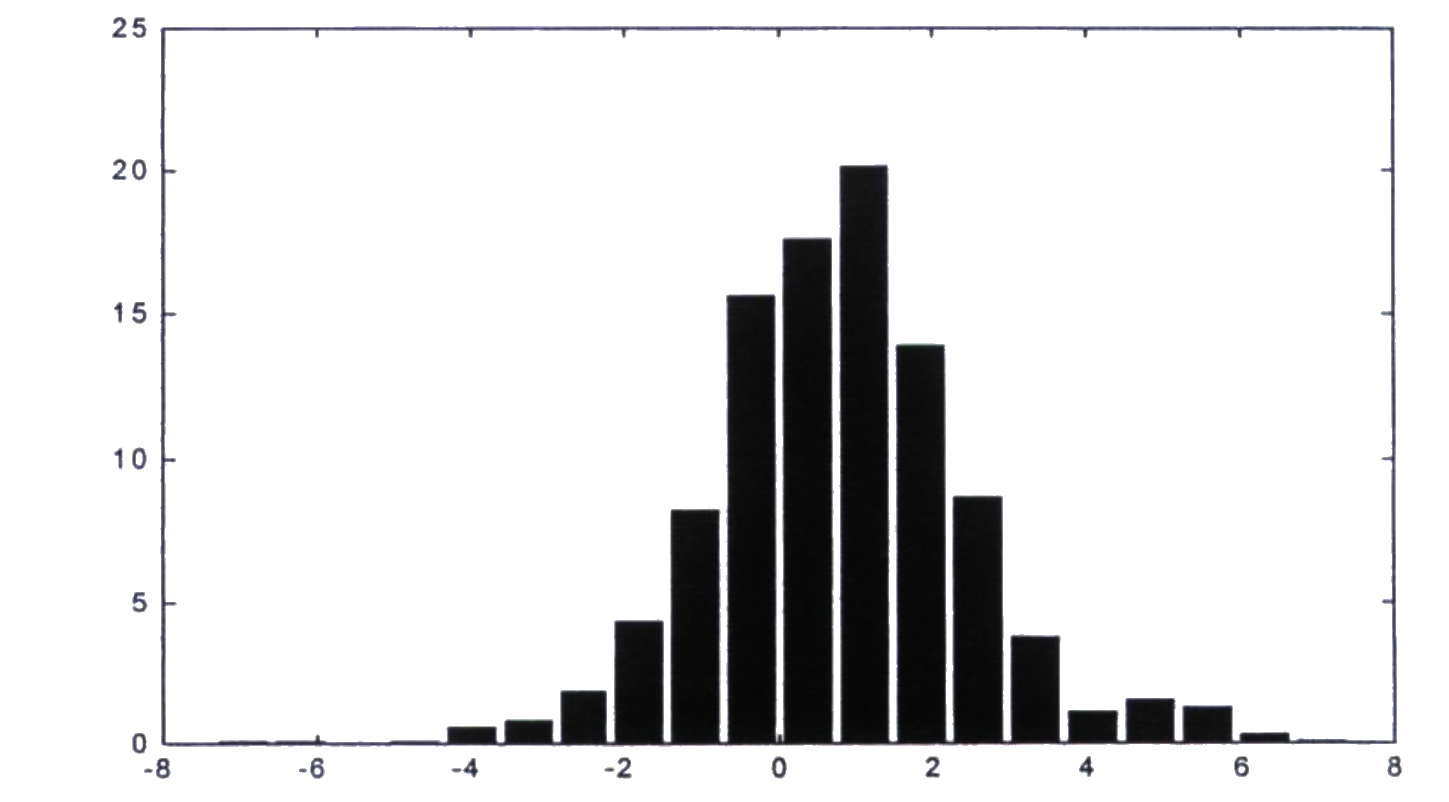
\includegraphics[width=\linewidth]{figures/ch08/nevo00_fig1_mushy.png}
\caption{Taste for sogginess (Mushy coefficient)}
\end{subfigure}

\medskip
\begin{subfigure}[t]{0.72\textwidth}
\centering
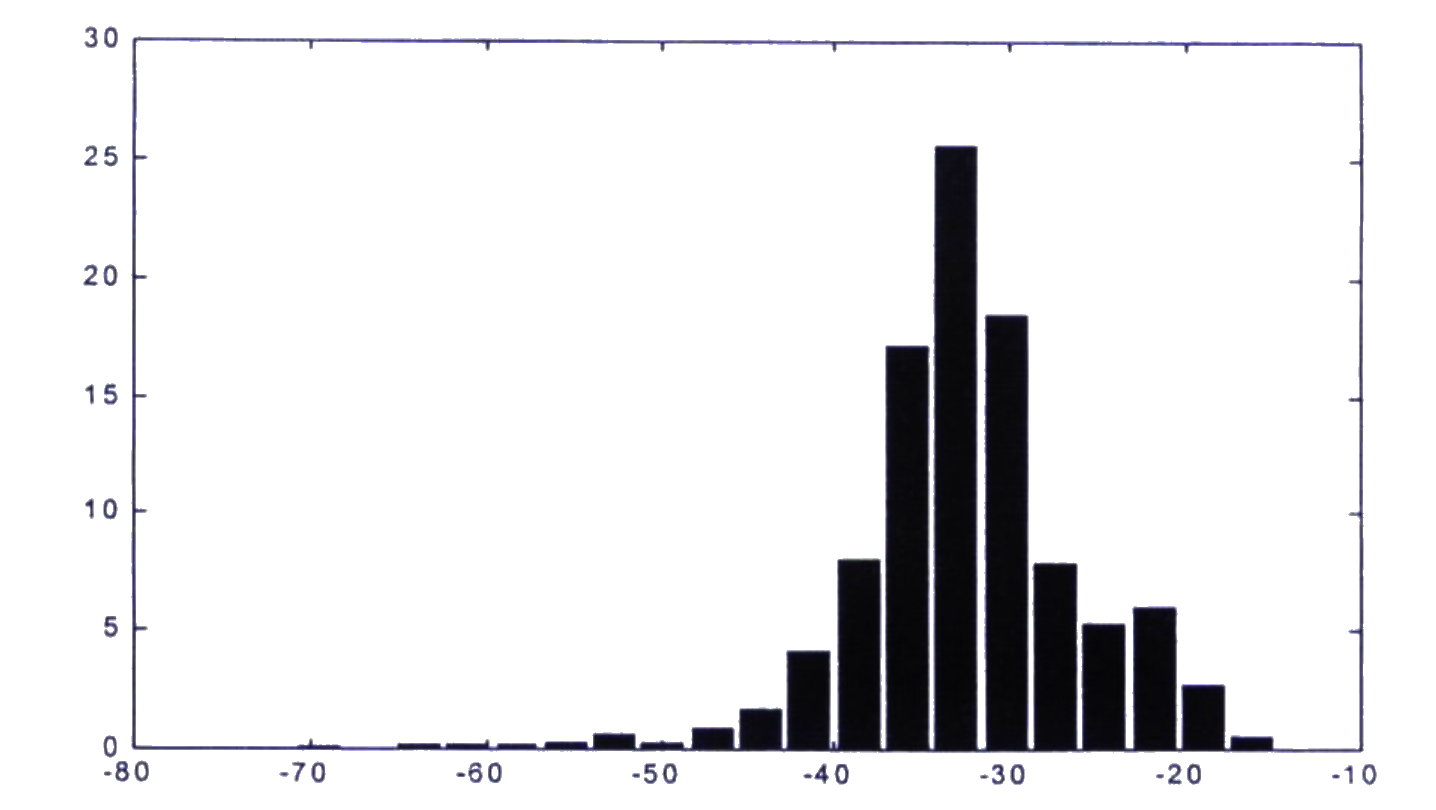
\includegraphics[width=\linewidth]{figures/ch08/nevo00_fig2_price.png}
\caption{Price coefficient}
\end{subfigure}
\caption{Frequency distributions (in percent) of two individual coefficients implied
by the estimates in \cref{tab:08-nevo00-results}. Panel (a) has mass below zero for consumers who prefer
crunchy cereal. Panel (b) is skewed because the empirical distribution of demographics drives it. Source:
\citet{Nevo2000a}, Figures 1 and 2.}
\label{fig:08-nevo00-dists}
\end{figure}

\casehead{Demographics against unobserved tastes}
The standard deviations are small relative to the demographic effects. Nevo computes the share of the
variance of each estimated coefficient explained by demographics, and all these shares exceed 90 percent
(p.~541). He reads this with care. It does not show that demographics explain all heterogeneity. It shows
that the data reject the assumed normal distribution of unobserved tastes. Other work had found that
purchase histories \citep{RossiMcCullochAllenby1996} and second-choice data \citep{BerryLevinsohnPakes2004}
explain heterogeneity beyond demographics (footnote 27). A second explanation is the absence of
choice-set variation across markets in these data, which BLP's data have. Such variation helps identify
the variance of the random shocks (\cref{sec:08-nevo00-practice}). Nevo notes that this explanation
accounts for imprecision, but not for the low point estimates or for the significance of the demographic
effects.

\casehead{Specification tests}
Nevo tests the logit against the full model by testing that all nonlinear parameters are jointly zero,
and the hypothesis is easily rejected (footnote 28). The GMM objective is 14.9 with 7 degrees of freedom.
If the objective is scaled as Hansen's $J$ statistic, this value exceeds the 95th percentile of the
$\chi^2(7)$ distribution, which is 14.07. The $p$-value is about 0.04 (our calculation), a marginal
rejection of the overidentifying restrictions. Nevo does not discuss this statistic.

\casehead{Elasticities}
\Cref{tab:08-nevo00-elas} reproduces Nevo's Table II. It reports the median over the 94 markets of each
own and cross elasticity for nine of the 24 brands, with each brand's characteristics. Entry $(i,j)$ is
the percentage change in the share of row brand $i$ for a one-percent change in the price of column
brand $j$.

\begin{table}[htbp]
\centering
\caption{Median own- and cross-price elasticities, synthetic cereal data (Nevo 2000a, Table II)}
\label{tab:08-nevo00-elas}
\footnotesize
\setlength{\tabcolsep}{3.3pt}
\begin{tabular}{@{}rrrrrrrrrrrr@{}}
\toprule
 & \multicolumn{2}{c}{Characteristics} & \multicolumn{9}{c}{Price of brand} \\
\cmidrule(lr){2-3}\cmidrule(l){4-12}
Brand & Sugar & Mushy & 1 & 2 & 3 & 4 & 5 & 14 & 15 & 19 & 24 \\
\midrule
1  & 2  & 1 & $-2.1689$ & 0.0562 & 0.2429 & 0.1161 & 0.0645 & 0.0596 & 0.0611 & 0.0759 & 0.2375 \\
2  & 18 & 1 & 0.1119 & $-3.4505$ & 0.1302 & 0.0924 & 0.1905 & 0.2305 & 0.2606 & 0.4380 & 0.1165 \\
3  & 4  & 1 & 0.2715 & 0.0674 & $-2.9208$ & 0.1083 & 0.0709 & 0.0627 & 0.0684 & 0.0944 & 0.2237 \\
4  & 3  & 0 & 0.1868 & 0.0736 & 0.1501 & $-3.2709$ & 0.1470 & 0.1557 & 0.1564 & 0.1037 & 0.2670 \\
5  & 12 & 0 & 0.0965 & 0.1540 & 0.0947 & 0.1326 & $-5.5116$ & 0.2852 & 0.3085 & 0.2988 & 0.1715 \\
\addlinespace
6  & 14 & 0 & 0.0699 & 0.1642 & 0.0698 & 0.1123 & 0.2518 & 0.3628 & 0.3971 & 0.3513 & 0.1369 \\
7  & 3  & 1 & 0.2828 & 0.0606 & 0.2390 & 0.1035 & 0.0648 & 0.0563 & 0.0598 & 0.0865 & 0.2225 \\
8  & 4  & 0 & 0.1743 & 0.0789 & 0.1476 & 0.1622 & 0.1524 & 0.1620 & 0.1656 & 0.1180 & 0.2555 \\
9  & 14 & 0 & 0.0735 & 0.1704 & 0.0717 & 0.1128 & 0.2596 & 0.3586 & 0.3966 & 0.3443 & 0.1333 \\
10 & 1  & 0 & 0.2109 & 0.0643 & 0.1682 & 0.1665 & 0.1224 & 0.1199 & 0.1298 & 0.0817 & 0.2809 \\
\addlinespace
11 & 11 & 0 & 0.0967 & 0.1556 & 0.0890 & 0.1377 & 0.2426 & 0.3322 & 0.3427 & 0.2899 & 0.1769 \\
12 & 4  & 1 & 0.2711 & 0.0691 & 0.2339 & 0.1121 & 0.0735 & 0.0662 & 0.0704 & 0.0985 & 0.2260 \\
13 & 3  & 1 & 0.2827 & 0.0597 & 0.2390 & 0.0983 & 0.0632 & 0.0554 & 0.0582 & 0.0866 & 0.2189 \\
14 & 13 & 0 & 0.0834 & 0.1825 & 0.0786 & 0.1247 & 0.2697 & $-3.8393$ & 0.3922 & 0.3380 & 0.1600 \\
15 & 13 & 0 & 0.0889 & 0.1763 & 0.0814 & 0.1256 & 0.2491 & 0.3542 & $-4.3982$ & 0.3383 & 0.1582 \\
\addlinespace
16 & 16 & 1 & 0.1430 & 0.2282 & 0.1523 & 0.0873 & 0.1447 & 0.1442 & 0.1702 & 0.3270 & 0.1264 \\
17 & 10 & 0 & 0.1138 & 0.1399 & 0.1005 & 0.1466 & 0.2172 & 0.2867 & 0.2912 & 0.2498 & 0.1875 \\
18 & 3  & 0 & 0.1900 & 0.0717 & 0.1542 & 0.1656 & 0.1362 & 0.1508 & 0.1578 & 0.1026 & 0.2660 \\
19 & 20 & 1 & 0.0944 & 0.2691 & 0.1130 & 0.0771 & 0.2163 & 0.2618 & 0.3107 & $-3.3335$ & 0.1013 \\
20 & 7  & 0 & 0.1420 & 0.0999 & 0.1270 & 0.1546 & 0.1791 & 0.2074 & 0.2080 & 0.1628 & 0.2251 \\
\addlinespace
21 & 14 & 0 & 0.0773 & 0.1706 & 0.0741 & 0.1160 & 0.2534 & 0.3573 & 0.3794 & 0.3530 & 0.1416 \\
22 & 6  & 0 & 0.1500 & 0.0950 & 0.1283 & 0.1602 & 0.1797 & 0.2096 & 0.2085 & 0.1530 & 0.2311 \\
23 & 12 & 0 & 0.0854 & 0.1561 & 0.0815 & 0.1307 & 0.2559 & 0.3484 & 0.3753 & 0.3154 & 0.1608 \\
24 & 0  & 0 & 0.2249 & 0.0548 & 0.1731 & 0.1619 & 0.1110 & 0.1044 & 0.1114 & 0.0733 & $-4.1215$ \\
\midrule
\multicolumn{3}{@{}l}{Outside good} & 0.0303 & 0.2433 & 0.0396 & 0.0552 & 0.2279 & 0.3349 & 0.3716
 & 0.3896 & 0.0399 \\
\bottomrule
\end{tabular}

\smallskip
\begin{minipage}{0.97\linewidth}
\footnotesize
Notes: Source: \citet{Nevo2000a}, Table II (p.~542). Entry $(i,j)$ is the percentage change in the
market share of row brand $i$ for a one-percent change in the price of column brand $j$. Each entry is the
median over the 94 markets. Only nine of the 24 columns are printed in the source.
\end{minipage}
\end{table}

\casehead{Reading Table II}
Own elasticities among the printed columns range from $-2.17$ (brand 1) to $-5.51$ (brand 5). Cross
elasticities within a column vary with characteristics, unlike the logit, which forces a constant column.
Nevo summarizes this by the ratio of the largest to the smallest cross elasticity in a column, which he
reports varies from 9 to 3 (p.~543).\footnote{Among the nine printed columns, the ratio ranges from 2.2
(brand 4) to 6.8 (brand 15) by our calculation. Nevo's range presumably covers all 24 columns, most of
which are not printed.} A column with a ratio near one shows that the characteristics are too weak to
break the logit pattern for that brand. Nevo suggests the diagnostic can guide which characteristics to
add.

Brands with the same characteristics have nearly identical rows. Nevo points to brands 14 and 15, which
both have Sugar 13 and Mushy 0. The table contains five more such groups: brands 3 and 12, 4 and 18, 5
and 23, 7 and 13, and 6, 9 and 21. The following result explains the pattern.

\begin{proposition}[Products with identical heterogeneous utility]\label{prop:08-nevo00-identical}
Suppose products $j$ and $j'$ have $\mu_{ij}=\mu_{ij'}$ for every consumer $i$. Then for every inside product
$k\notin\{j,j'\}$, the elasticities of $j$ and $j'$ with respect to $p_k$ are equal. Moreover, the diversion from $k$ to $j$ and to $j'$ is in proportion to their shares,
$\frac{D_{kj}}{D_{kj'}}=\frac{s_j}{s_{j'}}$.
\end{proposition}

\begin{proof}
From \eqref{eq:08-individual-share}, $\frac{s_{ij}}{s_{ij'}}=e^{\delta_j-\delta_{j'}}\equiv c$ for every $i$.
Integrating gives $s_j=c\,s_{j'}$, so $\frac{s_{ij}}{s_j}=\frac{s_{ij'}}{s_{j'}}$ for every $i$. The cross
elasticity with respect to $p_k$ is
\begin{equation*}
\varepsilon_{jk}=\frac{p_k}{s_j}\int\alpha_is_{ij}s_{ik}\,\dd F
 =p_k\int\alpha_i\frac{s_{ij}}{s_j}\,s_{ik}\,\dd F ,
\end{equation*}
and the last expression is the same for $j$ and $j'$. For the diversion ratios,
the common denominator $\big|\frac{\partial s_k}{\partial p_k}\big|$ cancels, so
\begin{equation*}
\frac{D_{kj}}{D_{kj'}}=\frac{\int\alpha_is_{ij}s_{ik}\,\dd F}{\int\alpha_is_{ij'}s_{ik}\,\dd F}
 =c=\frac{s_j}{s_{j'}} .
\end{equation*}
\end{proof}

In the application price carries a random coefficient, so $\mu_{ij}$ includes the price term. Two brands
with the same Sugar and Mushy but different prices have slightly different $\mu$. Their rows are
therefore close but not identical, as in brands 14 and 15 (0.0834 against 0.0889 in column 1, 0.2697
against 0.2491 in column 5). The second part of the proposition shows that the random coefficients model
keeps the IIA property among products that differ only in $\xi$. This is the clone problem of
\cref{sec:08-practice}.

The outside-good row varies a lot, from 0.0303 for brand 1 to 0.3896 for brand 19. It rises with the
brand's sugar content. Across the nine printed columns, its correlation with Sugar is 0.90 (our
calculation). Table I suggests why. Richer consumers value inside goods more (the Constant-Income
interaction is 3.089) and value sugar less (the Sugar-Income interaction is $-0.193$). Buyers of sugary
brands are therefore poorer on average, closer to the margin of buying nothing, and they move to the
outside good when prices rise.

\subsection{Lessons, extensions and assessment}\label{sec:08-nevo00-lessons}

\casehead{Lessons from the application}
Nevo stresses economic significance over statistical significance, because most coefficients are
imprecise. He attributes the imprecision to the simplifications made for teaching. More data, more
simulation draws than $n_s=20$, better simulation methods or a supply side would improve efficiency
(p.~540). The application shows four things a user of the method should expect. Demographic interactions
can carry most of the heterogeneity. Distributions of individual coefficients inherit the shape of the
demographic distribution. Elasticity matrices depart clearly from the logit pattern but only as far as
the characteristics allow. Without choice-set variation the standard deviations are hard to pin down.

\casehead{Extensions}
Nevo's Section 5 lists five directions.
\begin{itemize}
\item \emph{Supply side.} In the guide the supply side only motivates the instruments. Specifying it
  adds moment conditions with little extra programming for standard static models (\cref{sec:08-supply}).
  It raises efficiency at the cost of more structure.
\item \emph{Consumer-level data.} With individual choices, models are usually estimated by maximum
  likelihood or simulated moments, as in \citet{Goldberg1995}, \citet{RossiMcCullochAllenby1996} and
  \citet{McFaddenTrain2000}. The mean utilities can be estimated from the micro data and then treated like
  inverted mean utilities, with standard errors that account for their estimation. Endogeneity can
  persist with micro data, because optimal choice from a menu can create it \citep{Kennan1989} and common
  unobserved characteristics remain. Combining micro and aggregate data adds moments, as in
  \citet{Petrin2002} and \citet{BerryLevinsohnPakes2004} (\cref{sec:08-micro,sec:08-blp04,sec:08-goldberg}).
\item \emph{Alternative methods.} Multi-level demand systems use separability to model a category, its
  segments and the brands within each segment, each with a flexible form such as the almost ideal demand
  system \citep{DeatonMuellbauer1980a,HausmanLeonardZona1994}. They become impractical when segments
  contain more than a handful of brands (\cref{ch:aids}).
\item \emph{Dynamics.} The static demand model can feed dynamic models of firm behavior
  \citep{PakesMcGuire1994}, and dynamic models could endogenize characteristics and supply new
  identifying conditions. Demand-side dynamics are better studied with consumer-level data
  \citep{ErdemKeane1996}.
\item \emph{Instruments.} Nevo closes with a warning. Identification rests on adequate exogenous
  instruments, and researchers should not let the technical fireworks distract from this basic and
  difficult problem (p.~546).
\end{itemize}

\casehead{Limitations and critiques}
The application cannot answer any substantive question, because its data are synthetic. Its small number
of draws makes simulation error a real concern (\cref{sec:08-simulation}). The absence of choice-set
variation weakens identification of $\Sigma$, as Nevo notes. The guide's code and data became a standard
test case for later computational work. \citet[Section~6.2]{DubeFoxSu2012} used the cereal data to show how a
loose inner-loop tolerance distorts estimates. They also note that a loose outer-loop tolerance left the guide's
reported estimates short of a local optimum. \citet[p.~39]{KnittelMetaxoglou2014} adapted the
guide's code to study how estimates on these data vary with optimizers and starting values.
\citet[Section~6]{ConlonGortmaker2020} distribute the data with their software and replicate the guide's model on
them. They find that tight optimization tolerances remove this dispersion (\cref{sec:08-practice}).

\casehead{Contribution}
The guide made the method usable. It translated BLP's estimator into explicit steps, explained the role
of each assumption, and gave rules for market size, instruments and brand effects. The posted data and
code let a generation of researchers reproduce every number before applying the method to their own
markets. Its notation, with $\theta_1$, $\theta_2$, $\Pi$ and $\Sigma$, is the notation of this chapter.
Its most durable advice is that heterogeneity should be modeled with outside information wherever possible
and that instruments deserve more attention than computation. \Cref{sec:08-nevo01} turns to Nevo's own
application of the method to market power in ready-to-eat cereal.

\section{Case study: Nevo (2001), market power in ready-to-eat cereal}\label{sec:08-nevo01}

\citet{Nevo2001} applies the random coefficients logit model to a question the model was built to answer. Are
the high price-cost margins of the ready-to-eat cereal industry the result of collusion? The paper estimates
brand-level demand for 25 cereals from city-level scanner data. It then computes the margins that the estimated
demand implies under three models of conduct and compares them with accounting margins. The resulting
decomposition of margins into a differentiation effect, a portfolio effect and a collusion effect is the
paper's main methodological contribution. We follow the paper from its question to its contribution and
reproduce all of its main tables. \Cref{tab:08-nevo01-map} at the end of the section maps the study. Page
numbers refer to the journal article.\footnote{Nevo writes the
market-specific deviation of unobserved quality as $\Delta\xi_{jt}$ and the econometric error as
$\omega_{jt}$. We write $\tilde\xi_{jt}$ for both, because $\Delta$ is the matrix of share derivatives in this
book (\cref{sec:08-model}) and $\omega$ is the cost unobservable in \cref{sec:08-supply}. Nevo writes firm
profits as $\Pi_f$ and the GMM weighting matrix as $A^{-1}$. We write $\pi_f$ and $W$, because $\Pi$ is the
matrix of demographic interactions.}

\subsection{The question}\label{sec:08-nevo01-question}

Ready-to-eat (RTE) cereal combines high concentration, high price-cost margins, heavy advertising and frequent
introductions of new brands. These features made it a standard example of an oligopoly that avoids price
competition and channels rivalry into advertising and new products. Nevo (p.~307, n.~2) quotes the verdict of
\citet[p.~189]{Scherer1982}. In Scherer's words, ``the cereal industry's conduct fits well the model of price
competition-avoiding, non-price competition-prone oligopoly.'' The inference ran from high margins to soft price
competition. Nevo asks whether the inference survives once demand is measured with care.

The difficulty is that a high margin has three possible sources. The first is product differentiation. A brand
with loyal consumers faces inelastic demand and earns a margin even when its owner sets its price alone. The
second is the \emph{portfolio effect}. A firm that owns several brands internalizes the substitution among them
and prices each brand higher than separate owners would. The third is \emph{price collusion}, the joint setting
of prices across firms. Accounting data reveal at best the sum of the three. Nevo separates them by asking what
margin each conduct model implies, given the estimated demand, and which model reproduces the observed margin.
No cost data enter the computation of the predicted margins.

The answer is that multi-product Nash-Bertrand pricing at the current ownership structure matches the observed
margins. Joint profit maximization over the 25 brands predicts margins far above them. Nevo concludes that
prices are consistent with noncollusive conduct despite margins above 45\% (p.~308). The margins come from the
firms' portfolios of differentiated brands and from perceived quality built by advertising.

\subsection{The industry}\label{sec:08-nevo01-industry}

The industry began at the Battle Creek sanatorium of John Harvey Kellogg, who introduced ready-to-eat cereal as
a health food. Entrants soon followed. They included Charles William Post, a former patient of Kellogg, and
Quaker Oats, a company with origins in hot oatmeal. A Minneapolis milling company, later called General Mills,
and the National Biscuit Company, now Nabisco, also entered (pp.~309--310). By the late 1940s the industry was one of the most concentrated in the United States. In 1997
the U.S. market consumed about three billion pounds of cereal, roughly \$9 billion in sales (p.~310).

\Cref{tab:08-nevo-shares} reproduces the volume shares of the six main manufacturers from 1988 to 1992. The
top three firms (Kellogg, General Mills, Post) held between 71.5\% and 75.2\% of pounds sold, and the top six
held between 87.5\% and 95.3\%. Kellogg's share fell from 41.4\% to 33.7\% while General Mills rose from
22.0\% to 26.8\%. Private labels doubled their share, from 3.3\% to 7.6\%. The leaders have also been very
profitable. Nevo cites a ranking of Kellogg third among 1,285 U.S. nonfinancial corporations by profitability
(p.~310, n.~6). The leaders earned after-tax returns on cereal assets of 19.8\% over 1958--1970, and profits
averaged about 17\% of sales in the 1980s and early 1990s.

\begin{table}[htbp]
\centering
\caption{Volume market shares of RTE cereal manufacturers, 1988--1992 (percent)}
\label{tab:08-nevo-shares}
\footnotesize
\begin{tabular}{@{}lrrrrrr@{}}
\toprule
 & 88Q1 & 88Q4 & 89Q4 & 90Q4 & 91Q4 & 92Q4 \\
\midrule
Kellogg & 41.39 & 39.91 & 38.49 & 37.86 & 37.48 & 33.70 \\
General Mills & 22.04 & 22.30 & 23.60 & 23.82 & 25.33 & 26.83 \\
Post & 11.80 & 10.30 & 9.45 & 10.96 & 11.37 & 11.31 \\
Quaker Oats & 9.93 & 9.00 & 8.29 & 7.66 & 7.00 & 7.40 \\
Ralston & 4.86 & 6.37 & 7.65 & 6.60 & 5.45 & 5.18 \\
Nabisco & 5.32 & 6.01 & 4.46 & 3.75 & 2.95 & 3.11 \\
\addlinespace
C3 & 75.23 & 72.51 & 71.54 & 72.64 & 74.18 & 71.84 \\
C6 & 95.34 & 93.89 & 91.94 & 90.65 & 89.58 & 87.53 \\
Private label & 3.33 & 3.75 & 4.63 & 6.29 & 7.13 & 7.60 \\
\bottomrule
\end{tabular}

\smallskip
\begin{minipage}{0.80\linewidth}
\footnotesize Notes: Shares of pounds sold. C3 and C6 are the combined shares of the three and six largest
firms. Source: \citet{Nevo2001}, Table I, from the IRI Infoscan data base of the Food Marketing Policy Center,
University of Connecticut.
\end{minipage}
\end{table}

Two features of the industry shape the analysis. The first is the number of brands. There were more than 200
brands, with national shares ranging from 5\% (Kellogg's Corn Flakes, General Mills' Cheerios) to 1\% for the
25th brand and below 0.1\% for the 100th (p.~311). Only 80 new brands appeared between 1950 and 1972, while
the top six producers introduced 67 major brands in the 1980s alone. Brand proliferation was the core of the
Federal Trade Commission's ``shared monopoly'' complaint against Kellogg, General Mills and Post in the 1970s,
whose economic argument \citet{Schmalensee1978} laid out. The second feature is advertising. The
advertising-to-sales ratio was about 13\%, against 2--4\% in other food industries, and about 18\% for the
established brands that Nevo studies (p.~311).

Production is less simple than it looks. There are five basic methods (granulation, flaking, shredding,
puffing and extrusion), and extrusion in particular requires experience. A typical plant produces \$400
million of output a year, employs 800 workers and costs \$300 million to build (p.~311). Several brands are
produced in one plant to exploit economies of scale in packaging.

\Cref{tab:08-nevo-costs} reproduces Nevo's two cost tables. Panel A uses the Annual Survey of Manufactures.
The gross margin of price over average variable cost (materials, labor and energy) is 64.4\% of the value of
shipments for RTE cereal, against 26.5\% for all food industries. Panel B reports accounting estimates of
marginal cost per pound from a 1994 investment-bank report on Kellogg, as presented in testimony by
\citet{Cotterill1996}. The manufacturer's gross margin is 57.5\% of the manufacturer's price. It is about seven
points below the Census figure, which Nevo attributes to the difference between marginal and average cost
(p.~312). The last column expresses each item as a share of the retail price. The manufacturer's price is
80\% of the retail price, so the retail margin is 20\%, and the gross margin is
$0.575 \times 0.80 = 46.0\%$ of the retail price. This 46.0\% is the observed margin against which the
conduct models are tested in \cref{sec:08-nevo01-margins}.

\begin{table}[htbp]
\centering
\caption{Production costs and margins in RTE cereal}
\label{tab:08-nevo-costs}
\footnotesize
\begin{tabular}{@{}lrrrr@{}}
\toprule
\multicolumn{5}{@{}l}{\textit{Panel A. Aggregate estimates, Annual Survey of Manufactures, 1988--1992}} \\
\addlinespace
 & \multicolumn{2}{c}{RTE cereal (SIC 2043)} & \multicolumn{2}{c}{All food (SIC 20)} \\
\cmidrule(lr){2-3}\cmidrule(lr){4-5}
Item & M\$ & \% of value & M\$ & \% of value \\
\midrule
Value of shipments & 8,211 & 100.0 & 371,246 & 100.0 \\
Materials & 2,179 & 26.5 & 235,306 & 63.4 \\
Labor & 677 & 8.2 & 32,840 & 8.8 \\
Energy & 76 & 0.9 & 4,882 & 1.3 \\
Gross margin & & 64.4 & & 26.5 \\
\midrule
\multicolumn{5}{@{}l}{\textit{Panel B. Detailed estimates per pound}} \\
\addlinespace
Item & \$ per lb & \% of mfr.\ price & \% of retail price & \\
\midrule
Manufacturer price & 2.40 & 100.0 & 80.0 & \\
Manufacturing cost & 1.02 & 42.5 & 34.0 & \\
\quad Grain & 0.16 & 6.7 & 5.3 & \\
\quad Other ingredients & 0.20 & 8.3 & 6.7 & \\
\quad Packaging & 0.28 & 11.7 & 9.3 & \\
\quad Labor & 0.15 & 6.3 & 5.0 & \\
\quad Manufacturing costs (net of capital costs) & 0.23 & 9.6 & 7.6 & \\
Gross margin & & 57.5 & 46.0 & \\
Marketing expenses & 0.90 & 37.5 & 30.0 & \\
\quad Advertising & 0.31 & 13.0 & 10.3 & \\
\quad Consumer promotion (manufacturer coupons) & 0.35 & 14.5 & 11.7 & \\
\quad Trade promotion (retail in-store) & 0.24 & 10.0 & 8.0 & \\
Operating profits & 0.48 & 20.0 & 16.0 & \\
\bottomrule
\end{tabular}

\smallskip
\begin{minipage}{0.92\linewidth}
\footnotesize Notes: Panel A computes the gross margin as value of shipments minus materials, labor and energy,
a price-average variable cost margin relative to the manufacturer's price. In Panel B capital costs were
computed from Annual Survey of Manufactures data. The source is \citet{Cotterill1996}, who reports estimates
from a CS First Boston report on the Kellogg Company (October 1994). Source: \citet{Nevo2001}, Tables II and
III.
\end{minipage}
\end{table}

\subsection{Supply: three models of conduct}\label{sec:08-nevo01-supply}

The supply side is the multi-product Bertrand-Nash model of \cref{sec:08-supply}, applied market by market.
There are $F$ firms, and firm $f$ produces the subset $\mathcal{J}_f$ of the $J$ brands. Its profit in a market of
size $M$ is $\pi_f = \sum_{j \in \mathcal{J}_f} (p_j - mc_j)\, M s_j(p) - C_f$, with $C_f$ the fixed cost. Nevo
assumes that a pure-strategy Bertrand-Nash equilibrium exists with strictly positive prices. The first-order
conditions are \eqref{eq:08-foc} (p.~313), and stacking them as in \eqref{eq:08-foc-matrix} gives
\begin{equation}\label{eq:08-nevo-markup}
p - mc = -\big[(\Omega \odot \Delta)^{\T}\big]^{-1} s(p),
\end{equation}
where $\Omega$ is the ownership matrix and $\Delta$ the matrix of share derivatives. This is Nevo's equation
(1).\footnote{Nevo defines $S_{jr} = -\frac{\partial s_r}{\partial p_j}$ and the
matrix with elements $\Omega^*_{jr} S_{jr}$, which equals $-(\Omega\odot\Delta)^{\T}$. His equation (1), $p -
mc = \Omega^{-1}s(p)$ in his notation, is therefore identical to \cref{eq:08-nevo-markup}.} Given estimated
demand, the right side is known at the observed prices and shares. The equation therefore delivers the markup
of every brand, and with it the implied marginal cost $mc = p + [(\Omega\odot\Delta)^{\T}]^{-1}s$, without any
cost data.

The key step is to evaluate \cref{eq:08-nevo-markup} under ownership matrices other than the true one. Nevo
uses three.
\begin{enumerate}
\item \emph{Single-product firms}, $\Omega = I_J$. Each brand is priced by an agent who considers only its own
profit. The implied margins reflect product differentiation alone.
\item \emph{Current ownership}, $\Omega = \Omega^{\mathrm{co}}$, the actual ownership of the 25 brands by
Kellogg, General Mills, Post, Quaker and Nabisco. The implied margins add the portfolio effect.
\item \emph{Joint ownership}, $\Omega = \iota\iota^{\T}$ with $\iota$ a vector of ones. One agent prices all
25 brands, which corresponds to monopoly or perfect price collusion among them.
\end{enumerate}
The margin under single-product pricing measures differentiation. The difference between the current-ownership
and single-product margins measures the portfolio effect. The difference between the joint-ownership and
current-ownership margins bounds the increase that collusion could produce (p.~313). Each row answers a
counterfactual question about costs. If firms behaved according to conduct model $k$, what marginal costs would
rationalize the observed prices? Each set of implied costs yields implied margins
$L_j^{k} = \frac{p_j - mc_j^{k}}{p_j}$, and the test compares them with observed margins.

A rearrangement of the first-order condition shows what drives the differences between the three rows. Divide
\eqref{eq:08-foc} by $-\frac{\partial s_j}{\partial p_j} > 0$ and use the diversion ratio
$D_{jr} = -\big(\frac{\partial s_r}{\partial p_j}\big)\big(\frac{\partial s_j}{\partial p_j}\big)^{-1}$ of \cref{prop:08-diversion}:
\begin{equation}\label{eq:08-nevo-diversion}
p_j - mc_j = \frac{s_j}{-\frac{\partial s_j}{\partial p_j}} + \sum_{r \in \mathcal{J}_f,\, r \neq j}
D_{jr}\,(p_r - mc_r).
\end{equation}
Dividing by $p_j$ gives the multi-product Lerner decomposition of \cref{prop:08-blp-lerner}. The first term is the
single-product markup. The second adds the markups of co-owned products, weighted by the
fraction of $j$'s lost sales that each of them captures. Enlarging the set of jointly priced products adds
terms to the sum. The following proposition makes the ordering precise for any demand system with substitutes.

\begin{proposition}[Ownership and implied markups]\label{prop:08-nevo-ownership}
Fix prices and shares, and suppose that $\frac{\partial s_j}{\partial p_j} < 0$,
$\frac{\partial s_r}{\partial p_j} \geq 0$ for $r \neq j$, and $\sum_{r \neq j} D_{jr} < 1$ for every $j$,
where the sum runs over inside goods. For any ownership matrix $\Omega$, the first-order conditions have a
unique solution $m^{\Omega} = p - mc$. It satisfies $m^{\Omega}_j \geq s_j\big(-\frac{\partial s_j}{\partial
p_j}\big)^{-1} > 0$ for every $j$. If $\Omega' \geq \Omega$ element by element, then $m^{\Omega'} \geq m^{\Omega}$
element by element.
\end{proposition}

\begin{proof}
Let $b_j = s_j\big(-\frac{\partial s_j}{\partial p_j}\big)^{-1} > 0$ and let $\mathbf{D}$ be the $J\times J$ matrix with
zero diagonal and off-diagonal elements $D_{jr} \geq 0$. By \cref{eq:08-nevo-diversion}, the first-order
conditions are
\[
m = b + (\Omega \odot \mathbf{D})\, m .
\]
Each row sum of $\Omega \odot \mathbf{D}$ is at most $\sum_{r\neq j} D_{jr} < 1$. Hence the sup-norm of
$\Omega\odot\mathbf{D}$ is below one, its spectral radius is below one, and $I - \Omega\odot\mathbf{D}$ is
invertible with
\[
(I - \Omega\odot\mathbf{D})^{-1} = \sum_{n=0}^{\infty} (\Omega\odot\mathbf{D})^n .
\]
Every term of the series is a nonnegative matrix, so $m^{\Omega} = \sum_{n\geq 0} (\Omega\odot\mathbf{D})^n b
\geq b$, which proves the first two claims. If $\Omega' \geq \Omega$, then $\Omega'\odot\mathbf{D} \geq
\Omega\odot\mathbf{D} \geq 0$ element by element. Products of nonnegative matrices are monotone in their
factors, so $(\Omega'\odot\mathbf{D})^n \geq (\Omega\odot\mathbf{D})^n$ for every $n$, and summing gives
$m^{\Omega'} \geq m^{\Omega}$.
\end{proof}

The condition $\sum_{r\neq j} D_{jr} < 1$ says that some of $j$'s lost sales go to the outside good. It holds in
every logit-type model with an outside option. The proposition implies that the three rows of Nevo's table are
ordered for every brand. It also shows that the size of the portfolio and collusion effects depends on the
diversion ratios among the jointly priced brands. The logit model restricts those ratios severely. In the logit,
$D_{jr} = \frac{s_r}{1-s_j}$, and \cref{prop:08-logit-markup} shows that if the products in a set $\mathcal{G}$ are
priced jointly, every $j \in \mathcal{G}$ has the markup
\begin{equation}\label{eq:08-nevo-logit}
p_j - mc_j = \frac{1}{\alpha\,(1 - S_{\mathcal{G}})}, \qquad S_{\mathcal{G}} = \sum_{r \in \mathcal{G}} s_r .
\end{equation}

This formula explains why the logit cannot detect collusion in this market. Nevo defines the potential market
as one serving per person per day, so the outside good has a large share and the 25 brands have a small
combined share. By \eqref{eq:08-nevo-logit}, the ratio of the joint-ownership to the single-product markup of brand $j$ is
$\frac{1-s_j}{1-S_{\mathcal{G}}}$, which is close to one when $S_{\mathcal{G}}$ is small. The logit spreads the
sales that a brand loses over all brands in proportion to their shares, and most of them go to the outside
good. Nevo anticipates this point when he writes that, under the logit, substitution to the inside goods ``will
on average be downward biased'' because the outside share is large (p.~316).

\subsection{Demand}\label{sec:08-nevo01-demand}

A market $t$ is a city-quarter. Consumer $i$ in market $t$ obtains from brand $j$ the indirect utility (Nevo's
equation (2), p.~314)
\begin{equation}\label{eq:08-nevo01-utility}
u_{ijt} = x_j \beta_i - \alpha_i p_{jt} + \xi_j + \tilde\xi_{jt} + \epsilon_{ijt},
\qquad i = 1,\dots,I_t,\quad j = 1,\dots,J_t,\quad t = 1,\dots,T .
\end{equation}
Here $x_j$ is a $K$-dimensional row vector of observed characteristics, which do not vary across markets.
The term $\xi_j$ is the national mean valuation of unobserved characteristics, $\tilde\xi_{jt}$ is its city-quarter
deviation and $\epsilon_{ijt}$ is a type-I extreme value shock. The unobserved characteristics include a
vertical component (at equal prices every consumer weakly prefers a national brand to its generic copy) and
local merchandising other than national advertising. Firms and consumers observe all of them.

Tastes follow \eqref{eq:08-tastes} with $\nu_i \sim N(0, I_{K+1})$ (Nevo's equation (3)). The demographics $D_i$ are
drawn from the empirical distribution in the consumer's city, and $\Sigma$ is diagonal in the application. The
specification combines observed demographics with a parametric distribution for the rest of the heterogeneity,
and so relaxes the normality assumption on the distribution of tastes. The outside good gives
$u_{i0t} = \xi_0 + \pi_0 D_i + \sigma_0 \nu_{i0} + \epsilon_{i0t}$. Its mean $\xi_0$ is normalized to zero.
The terms $\pi_0$ and $\sigma_0$ cannot be separated from a demographic-varying intercept in
\eqref{eq:08-nevo01-utility}, so they are set to zero (p.~315), as in \cref{sec:08-normalization}.

Substituting the taste model into \eqref{eq:08-nevo01-utility} exactly as in \cref{sec:08-linear} gives
$u_{ijt} = \delta_{jt} + \mu_{ijt} + \epsilon_{ijt}$, with
\begin{equation}\label{eq:08-nevo-decomp}
\delta_{jt} = x_j\beta - \alpha p_{jt} + \xi_j + \tilde\xi_{jt},
\qquad \mu_{ijt} = \tilde x_{jt}(\Pi D_i + \Sigma\nu_i),
\end{equation}
Nevo's equation (4). Mean utility $\delta_{jt}$ collects the linear parameters $\theta_1 = (\alpha, \beta)$. The
deviation $\mu_{ijt}$ depends on the nonlinear parameters $\theta_2 = (\Pi, \Sigma)$. Consumers buy one unit of the
brand that gives the highest utility. Nevo defends the single-unit assumption by noting that most people eat one
brand at a time even when households buy several (p.~315, n.~13). The market share is the integral
\eqref{eq:08-share-integral} of the logit probabilities \eqref{eq:08-individual-share} over the distribution of
$(D_i, \nu_i)$ (Nevo's equation (5)). By \cref{prop:08-derivs}, the price elasticities, written with Nevo's sign
convention, are
\begin{equation}\label{eq:08-nevo-elas}
\eta_{jkt} = \frac{\partial s_{jt}}{\partial p_{kt}}\frac{p_{kt}}{s_{jt}} =
\begin{cases}
-\dfrac{p_{jt}}{s_{jt}} \displaystyle\int \alpha_i\, s_{ijt}(1 - s_{ijt})\,\dd P^*(D,\nu) & \text{if } j = k,\\[2ex]
\dfrac{p_{kt}}{s_{jt}} \displaystyle\int \alpha_i\, s_{ijt}\, s_{ikt}\,\dd P^*(D,\nu) & \text{otherwise},
\end{cases}
\end{equation}
where $s_{ijt}$ is the logit probability \eqref{eq:08-individual-share}.

Nevo explains why the logit is inadequate for his purpose (p.~316). Its cross elasticities depend only on
shares. Suppose that Quaker's Cap'n Crunch (a children's cereal) and Post's Grape Nuts (a simple-nutrition cereal)
have similar shares. A rise in the price of General Mills' Lucky Charms (a children's cereal) then diverts
equally to both. Intuition says it should divert more to the other children's cereal. Nested logit and the principles-of-differentiation GEV
model of \citet{BresnahanSternTrajtenberg1997} relax this, but only through an a priori segmentation. The random
coefficients model lets the composite error $\mu_{ijt} + \epsilon_{ijt}$ correlate with characteristics, so
substitution follows characteristics. It also lets own elasticities reflect the price sensitivity of each
brand's buyers. \citet{McFaddenTrain2000} show that such mixed logit models can approximate any random utility
model arbitrarily well.

\subsection{Data}\label{sec:08-nevo01-data}

Quantities and prices come from the IRI Infoscan data base held by the Food Marketing Policy Center at the
University of Connecticut. IRI collects weekly scanner data from a random sample of supermarkets with annual
sales above \$2 million, which account for 82\% of U.S. grocery sales (p.~337). The data are aggregated to the
brand, city and quarter. They cover up to 65 cities, with the number rising over time, from 1988Q1 to 1992Q4.
The sample consists of the 25 brands with the highest national shares in 1992Q4. Every brand except Post Honey
Bunches of Oats appears in all 1,124 city-quarters. Honey Bunches of Oats enters in 1989Q1 (p.~317). The
estimation sample has 27,862 brand-city-quarter observations. The 25 brands account for 43\% to 62\% of cereal
volume in each city-quarter and for 55\% to 60\% nationally.

The variables are constructed as follows (Appendix A, pp.~337--338). Volume is converted to servings using the
manufacturer's serving weight. The \emph{potential market} is one serving per person per day. The share of
brand $j$ is servings sold divided by potential servings, and the outside share is one minus the sum of the
inside shares. Price is dollar sales divided by servings, deflated by a regional urban consumer price index. It
is therefore an average real transaction price per serving at the register, which does not net out
manufacturers' coupons. Advertising is total national expenditure by brand and quarter across ten media, from
the Leading National Advertisers data base. Characteristics were collected from cereal boxes. They are
calories from fat, sugar, fiber, a dummy for cereal that gets soggy in milk (\emph{mushy}), and segment dummies
for all-family, kids, adults (taste-enhanced wholesome) and simple-health brands. Demographics are 40 draws per
city and year from the March Current Population Survey (CPS). Income is household income divided by household
size, and \emph{Child} indicates age below 16.

\Cref{tab:08-nevo-sumstats} reproduces the summary statistics. The mean price is 19.4 cents per serving. Brand
dummies account for 88.4\% of the variance of prices and city dummies for a further 5.3\%. Nevo concludes that,
after controlling for brands, most price variation is across cities (p.~317). This cross-city variation, part
exogenous and part correlated with demand shocks, is what identifies the price coefficient.

\begin{table}[htbp]
\centering
\caption{Summary statistics for Nevo's cereal data}
\label{tab:08-nevo-sumstats}
\footnotesize
\begin{tabular}{@{}lrrrrrrrr@{}}
\toprule
\multicolumn{9}{@{}l}{\textit{Panel A. Prices and market shares of the 25 brands}} \\
\addlinespace
 & & & & & & \multicolumn{3}{c}{Share of variance due to} \\
\cmidrule(lr){7-9}
Variable & Mean & Median & Std & Min & Max & Brand & City & Quarter \\
\midrule
Price (cents per serving) & 19.4 & 18.9 & 4.8 & 7.6 & 40.9 & 88.4\% & 5.3\% & 1.6\% \\
Advertising (M\$ per quarter) & 3.56 & 3.04 & 2.03 & 0 & 9.95 & 66.2\% & n.a. & 1.8\% \\
Share within cereal market (\%) & 2.2 & 1.6 & 1.6 & 0.1 & 11.6 & 82.3\% & 0.5\% & 0\% \\
\midrule
\multicolumn{9}{@{}l}{\textit{Panel B. Characteristics and demographics}} \\
\addlinespace
Variable & Mean & Median & Std & Min & Max & & & \\
\midrule
Calories & 137.6 & 120 & 36.32 & 110 & 220 & & & \\
Fat calories ($\div 100$) & 0.124 & 0.100 & 0.139 & 0 & 0.60 & & & \\
Sodium (\% RDA $\div 100$) & 0.087 & 0.090 & 0.042 & 0 & 0.150 & & & \\
Fiber (\% RDA $\div 100$) & 0.095 & 0.050 & 0.094 & 0 & 0.310 & & & \\
Sugar (g $\div 100$) & 0.084 & 0.070 & 0.060 & 0 & 0.200 & & & \\
Mushy (1 if soggy in milk) & 0.35 & n.a. & n.a. & 0 & 1 & & & \\
Serving weight (g) & 35.1 & 30 & 9.81 & 25 & 58 & & & \\
Income (\$, per person) & 13,083 & 10,475 & 11,182 & 14 & 275,372 & & & \\
Age (years) & 29.99 & 28 & 23.14 & 1 & 90 & & & \\
Child (1 if age $<16$) & 0.23 & n.a. & n.a. & 0 & 1 & & & \\
\bottomrule
\end{tabular}

\smallskip
\begin{minipage}{0.97\linewidth}
\footnotesize Notes: Panel A covers 27,862 brand-city-quarter observations. The last three columns give the
share of the variance explained by brand, city and quarter dummies. Advertising does not vary across cities,
and the paper prints a dash for its city share. Panel B: characteristics from cereal boxes, demographics from
CPS draws. Sources: \citet{Nevo2001}, Table IV (Panel A) and Table A(II) (Panel B).
\end{minipage}
\end{table}

\subsection{Estimation}\label{sec:08-nevo01-estimation}

Nevo follows the BLP algorithm of \cref{sec:08-gmm} with three differences (p.~318). The instruments differ,
and so does the identifying assumption behind them. Demand is identified without a functional form for supply,
whereas BLP's identification uses their supply equation. Brand fixed effects control for unobserved product
quality.

The estimator is the GMM estimator \eqref{eq:08-gmm-obj} based on the population moment
$\E[Z^{\T}\tilde\xi(\theta^*)] = 0$, where $Z$ stacks the instruments and $\theta^*$ is the true parameter (Nevo's
equation (6)). The structural error is computed in two steps. First, for given $\theta_2$, the share system
\eqref{eq:08-inv-system} is inverted in each market (Nevo's equation (7)), with $S_{\cdot t}$ denoting the observed
shares. The logit solution is $\delta_{jt} = \ln S_{jt} - \ln S_{0t}$. The random coefficients solution is computed by
the contraction of \cref{sec:08-inversion}. Second, the recovered mean utilities are regressed on the linear part of
the model. With brand and quarter dummies, the estimating equation is
\begin{equation}\label{eq:08-nevo-esteq}
\delta_{jt}(S_{\cdot t}; \theta_2) = d_j + \tau_{q(t)} + \gamma\, a_{jt} - \alpha\, p_{jt} + \tilde\xi_{jt},
\end{equation}
where $d_j = x_j\beta + \xi_j$ is the brand effect, $\tau_{q(t)}$ is a quarter effect and $a_{jt}$ is
advertising. The error is the city-quarter deviation $\tilde\xi_{jt}$, because the brand effect absorbs both
$x_j\beta$ and $\xi_j$. In the logit, \cref{eq:08-nevo-esteq} with $\delta_{jt} = \ln S_{jt}-\ln S_{0t}$ is a
linear regression. With $W = (Z^{\T}Z)^{-1}$, the GMM estimator is two-stage least squares (p.~319, n.~15).

The weighting matrix is computed in two steps (p.~319). The first step sets $W = (Z^{\T}Z)^{-1}$ and yields
$\theta^{(1)}$. The second step uses the heteroskedasticity-robust matrix $W_2$ of \cref{sec:08-weighting},
evaluated at the residuals $\tilde\xi_{jt}(\theta^{(1)})$. Further iterations changed the estimates only slightly. The nonlinear
search is simplified in two ways. The first-order conditions are linear in $\theta_1$, so $\theta_1$ is
concentrated out as in \cref{prop:08-concentrate}, and the search runs over $\theta_2$ alone. The search uses a
quasi-Newton method with an analytic gradient, which Nevo found much faster than the Nelder-Mead simplex used
by BLP. Shares are simulated with the 40 CPS draws per city and year (200 per city over the five years) and
independent normal draws of $\nu_i$ (p.~326, n.~25).

Standard errors use the usual GMM formulas \citep{Hansen1982} with a correction for simulation error. The
correction exploits the fact that the same simulation draws are used for all brands in a market (p.~319).
Confidence intervals for nonlinear functions of the parameters, such as elasticities and margins, come from a
parametric bootstrap. Nevo draws repeatedly from the estimated asymptotic distribution of the parameters and
recomputes the function at each draw. Table VIII uses 1,500 draws.

\subsection{Instruments and identification}\label{sec:08-nevo01-instruments}

\Cref{eq:08-nevo-markup} shows why prices are endogenous. Prices equal marginal cost plus a markup, and the markup depends
on the demand shocks. Nevo decomposes the price into a brand mean and a city-quarter deviation (his equation
(8), p.~320):
\begin{equation}\label{eq:08-nevo-price}
p_{jt} = mc_{jt} + f(\tilde\xi_{jt}, \dots)
= \big(\overline{mc}_j + \bar f_j\big) + \big(\widetilde{mc}_{jt} + \tilde f_{jt}\big).
\end{equation}
Brand dummies absorb the first bracket. The error in \cref{eq:08-nevo-esteq} is $\tilde\xi_{jt}$, and firms
observe it when they set prices, so the markup deviation $\tilde f_{jt}$ is correlated with it. Unless the cost
deviation $\widetilde{mc}_{jt}$ exactly cancels this correlation, prices are correlated with $\tilde\xi_{jt}$ and
least squares, linear or nonlinear, is inconsistent. If the cost deviation $\widetilde{mc}_{jt}$ does not offset the markup
response, prices covary positively with $\tilde\xi_{jt}$ and the estimate of $\alpha$ is biased toward zero
(\cref{sec:08-endogeneity}). The results confirm this direction.

\casehead{Why characteristic-based instruments fail here} The usual instruments of \cref{sec:08-instruments}
are functions of the characteristics of rival products. They assume that product locations are exogenous or
predetermined, and they work because a brand's markup depends on the distance to its neighbors. Nevo points to
a more basic problem in his data (p.~320). Each brand's characteristics are constant across cities and
quarters, and the choice set is the same everywhere. Functions of characteristics therefore vary only with the
choice set, which barely varies. With brand dummies in the regression the instrument matrix is nearly
singular. It is not exactly singular only because Honey Bunches of Oats is missing from some quarters (n.~17).
The brand dummies themselves can serve as instruments when they are left out of the regression. This is a
nonparametric way of using all the information in fixed characteristics, and column (iv) of
\cref{tab:08-nevo-logit} reports it.

\casehead{Prices in other cities} The main instruments follow \citet{Hausman1997}. Write a market as
$t = (c, q)$, city $c$ in quarter $q$, and let $R(c)$ be the census region of city $c$. The instrument for
brand $j$ in city $c$ averages the price of $j$ over the other cities of the region,
\[
z^{H}_{j c q'} = \frac{1}{|R(c)| - 1}\sum_{c' \in R(c),\, c' \neq c} p_{j c' q'} ,
\]
and Nevo uses it for all 20 quarters $q'$ (p.~321).\footnote{Nevo notes that the results
are essentially the same if only the regional average for the same quarter is used (p.~325, n.~21). He makes
no claim that the instruments are optimal (n.~18).} Two assumptions justify the instrument. The first is the
identifying assumption itself. After brand effects, time effects and demographics, the city-specific
valuations $\tilde\xi_{jcq}$ are independent across cities, though they may be correlated within a city. The
second is a cost structure with a common regional component. Suppose that
\[
mc_{jcq} = \bar c_j + \lambda_{j R(c) q} + e_{jcq},
\]
with cost shocks independent of the demand shocks. By \cref{eq:08-nevo-price}, the price of $j$ in another
city $c'$ is $p_{jc'q'} = mc_{jc'q'} + f_{jc'q'}$. Its markup depends on the demand shocks of city $c'$, which
are independent of $\tilde\xi_{jcq}$ by the first assumption. Its cost is independent of $\tilde\xi_{jcq}$ by
the second. Hence $\Cov(z^{H}_{jcq'}, \tilde\xi_{jcq}) = 0$, which is the exclusion restriction. For $q' = q$,
the prices $p_{jcq}$ and $p_{jc'q}$ share the regional cost shock $\lambda_{jR(c)q}$, so the instrument is
relevant. Distribution costs (transportation, shelf space and labor) are the plausible source of such common
regional cost variation.

The independence assumption can fail in two ways (p.~321). A national or regional demand shock correlates
valuations across cities. Nevo's example is the discovery that fiber reduces the risk of cancer, which would
raise the valuation of every fiber-rich brand everywhere. He replies that the sample consists of established
brands, which are less exposed to systematic shocks, and that time dummies absorb aggregate shocks to cereal.
The second failure is local advertising or promotion coordinated across cities within a region. Nevo replies
that IRI cities are mostly larger than metropolitan areas and census regions are large. Firms also plan their
strategies on IRI's city-level geography.

\casehead{Cost proxies} Because the plausibility of these assumptions is an empirical matter, Nevo also uses
direct proxies for city-level marginal cost (pp.~321--322). Production and packaging costs vary little and are
captured by the brand dummies. Distribution costs are proxied by region dummies (transportation), city density
(the cost of space) and average earnings in the supermarket sector from the CPS Monthly Earnings Files
(labor). A persistent regional taste difference beyond demographics, such as a western preference for natural
cereals, would invalidate the region dummies. If both instrument sets give similar estimates, neither failure
is likely to be large.

\casehead{Identification of the nonlinear parameters} The price instruments identify $\alpha$. The parameters
in $\Pi$ are identified mainly by cross-city variation in the distribution of demographics. Cities with more
children or higher incomes should show different shares and different responses to price, in the directions
that $\Pi$ predicts. The standard deviations in $\Sigma$ would be identified by changes in the choice set, but
Nevo's choice set is almost fixed. He notes that this can explain their large standard errors, though not their
small point estimates (p.~330, n.~27). \Cref{sec:08-instruments} discusses this identification argument in
general.

\subsection{Brand fixed effects and the minimum-distance step}\label{sec:08-nevo01-md}

Brand dummies are Nevo's main departure from earlier work (pp.~322--323). They improve the fit of mean utility,
while substitution patterns are still driven by characteristics through $\mu_{ijt}$. They also remove the
correlation between price and the national unobserved quality $\xi_j$, the main motivation of
\citet{Berry1994}, without any instrument. Two objections arise. Brand dummies add parameters, but their number
grows with $J$ and not $J^2$, so the discrete-choice reduction of dimensionality survives. They are linear
parameters, so they add no computational burden.

The price of brand dummies is that $\beta$ is no longer estimated directly. Nevo recovers it by the
minimum-distance procedure of \citet{Chamberlain1982}, the generalized least squares regression \eqref{eq:08-md} of
the estimated brand effects on the fixed characteristics derived in \cref{sec:08-brand-fe}. Here the
``observations'' are the 25 brands. The restricted model, which sets $\xi_b = 0$, is tested by Chamberlain's
statistic with $J - K$ degrees of freedom. The assumption $\E[\xi_b\mid \bm{X}_b] = 0$ is the one that justifies
characteristic-based instruments. Here it serves only to recover the taste means and does not affect the price
coefficient (p.~322, n.~19).

\subsection{Results from the logit model}\label{sec:08-nevo01-logit}

The logit is inadequate for measuring market power, but it is cheap and shows how much instruments matter.
\Cref{tab:08-nevo-logit} reproduces Nevo's Table V. Every column regresses $\ln S_{jt} - \ln S_{0t}$ on price,
advertising and quarter dummies.

\begin{table}[htbp]
\centering
\caption{Logit demand for RTE cereal}
\label{tab:08-nevo-logit}
\scriptsize
\setlength{\tabcolsep}{2.4pt}
\begin{tabular}{@{}lrrrrrrrrrr@{}}
\toprule
 & \multicolumn{3}{c}{OLS} & \multicolumn{7}{c}{IV (2SLS)} \\
\cmidrule(lr){2-4}\cmidrule(l){5-11}
Variable & (i) & (ii) & (iii) & (iv) & (v) & (vi) & (vii) & (viii) & (ix) & (x) \\
\midrule
Price & $-$4.96 & $-$7.26 & $-$7.97 & $-$8.17 & $-$17.57 & $-$17.12 & $-$22.56 & $-$23.77 & $-$23.37 & $-$23.07 \\
 & (0.10) & (0.16) & (0.15) & (0.11) & (0.50) & (0.49) & (0.51) & (0.53) & (0.47) & (1.17) \\
Advertising & 0.158 & 0.026 & 0.026 & 0.157 & 0.020 & 0.020 & 0.018 & 0.017 & 0.018 & 0.013 \\
 & (0.002) & (0.002) & (0.002) & (0.002) & (0.002) & (0.002) & (0.002) & (0.002) & (0.002) & (0.002) \\
Log median income & & & 0.89 & & & & 1.06 & 1.13 & 1.12 & \\
 & & & (0.02) & & & & (0.02) & (0.02) & (0.02) & \\
Log median age & & & $-$0.423 & & & & $-$0.063 & 0.003 & $-$0.007 & \\
 & & & (0.052) & & & & (0.059) & (0.062) & (0.061) & \\
Median HH size & & & $-$0.126 & & & & $-$0.053 & $-$0.036 & $-$0.038 & \\
 & & & (0.027) & & & & (0.029) & (0.031) & (0.031) & \\
\addlinespace
Fit / overid.\ test & 0.54 & 0.72 & 0.74 & 436.9 & 168.5 & 181.2 & 83.96 & 82.95 & 85.87 & 15.06 \\
 & & & & (26.30) & (30.14) & (16.92) & (30.14) & (16.92) & (42.56) & (42.56) \\
First-stage $R^2$ & & & & 0.889 & 0.908 & 0.908 & 0.910 & 0.909 & 0.913 & 0.952 \\
First-stage $F$ & & & & 5119 & 124 & 288 & 129 & 291 & 144 & 180 \\
Instruments & & & & brand & prices & cost & prices & cost & prices, & prices, \\
 & & & & dummies & & & & & cost & cost \\
\addlinespace
Brand dummies & no & yes & yes & no & yes & yes & yes & yes & yes & yes \\
City dummies & no & no & no & no & no & no & no & no & no & yes \\
\bottomrule
\end{tabular}

\smallskip
\begin{minipage}{0.97\linewidth}
\footnotesize Notes: Dependent variable $\ln S_{jt} - \ln S_{0t}$, 27,862 observations. All regressions include
quarter dummies. Columns (i) and (iv) include the product characteristics (calories from fat, sugar, fiber,
mushy and segment dummies). Asymptotically robust standard errors in parentheses. The fit row reports the
adjusted $R^2$ for OLS and an overidentification test statistic for IV, with the 5\% rejection threshold in
parentheses. The thresholds are the 0.95 quantiles of $\chi^2$ with 16, 19, 9 and 29 degrees of freedom. ``Prices'' are average regional prices of the brand in other cities, and ``cost'' are the cost
proxies. Source: \citet{Nevo2001}, Table V.
\end{minipage}
\end{table}

\casehead{OLS} Column (i) includes characteristics but no brand dummies, so its error contains $\xi_j$. The
price coefficient is $-4.96$. Adding brand dummies in columns (ii) and (iii) raises it to $-7.26$ and $-7.97$,
a large and significant change. The direction of the change indicates that, in these data, brands with high
unobserved quality are both popular and expensive, which biases the column (i) coefficient toward zero. Even column (iii) implies a mean own elasticity of only $-1.53$ (median
$-1.50$, standard deviation 0.39). Its implied demand is inelastic for 5.5\% of observations (p.~323), which no
profit-maximizing firm would choose. The coefficients on characteristics in column (i) are not reported in the
table.\footnote{With standard errors in parentheses, they are constant $-4.44$ (0.04), fat calories 0.17
(0.04), sugar 2.7 (0.09), mushy $-0.12$ (0.011) and fiber 0.04 (0.06). The segment dummies are 0.53 (0.02)
for all-family, 0.47 (0.02) for kids and 0.53 (0.02) for health (p.~323, n.~20).}

\casehead{Instrumental variables} Column (iv) uses brand dummies as instruments without brand dummies in the
regression, which mimics characteristic-based identification. Its price coefficient, $-8.17$, nearly doubles
that of column (i) but almost equals the OLS coefficient with brand dummies. Column (v) instruments with
regional prices. The coefficient rises to $-17.57$, and every brand-city-quarter demand becomes elastic. The
mean own elasticity is $-3.38$ (median $-3.30$, standard deviation 0.85, p.~325). Column (vi) uses the cost
proxies instead and gives a similar $-17.12$. The two instrument sets rest on different assumptions and still
agree.

Adding city-level demographics raises the price coefficient to between $-22.56$ and $-23.77$ in columns (vii)
to (ix). Nevo reads this through the threat discussed above. If city valuations depend on demographics that are
correlated within regions, omitting demographics makes both instrument sets invalid. Adding them removes that
omitted-variable bias and improves the overidentification statistic, from 168.5 to 83.96 for the price
instruments. The value of cereal rises with income, while age and household size are insignificant. Column (x)
adds city fixed effects and leaves the price coefficient at $-23.07$. With city effects, identification comes
from variation over time within cities, so the results are not driven by cross-sectional differences alone
(n.~22).

The overidentification test rejects in every IV column except (x). Nevo notes that with 27,862 observations a
$\chi^2$ test rejects almost any model (pp.~325--326). He also notes that the coefficients do not change
from (ix) to (x), where city effects make the test pass. He concludes that the instruments are valid once demographics are
controlled for in a rich enough way, which the full model does. The first-stage $R^2$ exceeds 0.88 and the
first-stage $F$ statistics range from 124 to 5,119, so the instruments are not weak in the usual sense.

Nevo's Table B(I) reports the first stages behind columns (v) to (x) (p.~339). Each includes the exogenous
regressors of its column and region dummies. Both cost proxies enter with the expected positive sign and are
precisely estimated. City density has coefficients of 0.152 (standard error 0.017) in column (vi), 0.146 (0.018)
in (viii), 0.305 (0.019) in (ix) and 0.209 (0.010) in (x). Supermarket wages have coefficients of 0.172 (0.023),
0.196 (0.023), 0.182 (0.023) and 0.046 (0.018) in the same columns. The regional prices enter with one coefficient
for each of the 20 quarters. These coefficients take both signs, from $-0.477$ to $0.536$, and most are several
standard errors from zero. With 20 such instruments, the $F$ statistics measure their joint strength better than
any single coefficient does.

Advertising is significant. Its coefficient falls from 0.158 to about 0.02 once brand dummies are included,
because popular brands with high $\xi_j$ also advertise more. The implied mean advertising elasticity is about
0.06. Nevo calls this low, an order of magnitude below what a Dorfman-Steiner condition requires (p.~326).

The Dorfman-Steiner condition is the advertising analogue of the Lerner rule \citep{DorfmanSteiner1954}. Consider a single-product firm with
demand $q(p, A)$, where $A$ is advertising expenditure, constant marginal cost $c$ and profit $(p - c)\,q(p, A) -
A$. The first-order condition for advertising is $(p - c)\frac{\partial q}{\partial A} = 1$. Multiplying both
sides by $\frac{A}{pq}$ gives
\begin{equation*}
  \frac{A}{pq} = \frac{p - c}{p}\,\varepsilon_A, \qquad \varepsilon_A = \frac{\partial q}{\partial A}\,\frac{A}{q}.
\end{equation*}
The advertising-to-sales ratio equals the Lerner index times the advertising elasticity $\varepsilon_A$. Nevo
does not report the inputs behind his comparison. Take advertising-to-sales ratios of 13\% to 18\% (p.~311), which we read as
shares of manufacturer sales. On the same basis the margin bounds of \cref{sec:08-nevo01-margins} are about
39\% (the 31\% retail-price gap divided by 0.80) and 64.4\%. The condition then requires $\varepsilon_A$
between about 0.20 and 0.46, three to eight times the estimate (our calculation). The
benchmark is static and treats each brand alone. Advertising that also raises demand in later quarters or for
the firm's other brands changes the identity.

Nevo attributes the gap to measurement error in the advertising data (p.~326). He does not instrument for
advertising. It varies by brand
and quarter but not by city, and its coefficient does not move when price is instrumented, which suggests
little feedback onto the price coefficient (n.~24).

\subsection{Results from the random coefficients model}\label{sec:08-nevo01-full}

\Cref{tab:08-nevo-full} reproduces Table VI, the preferred specification. The instruments are the regional
prices for all quarters together with the cost proxies. Characteristics interact with four demographics:
income, income squared, age and the child dummy. Income is household income per person
(\cref{tab:08-nevo-sumstats}). The paper does not report how income and its square are transformed, scaled or
centered in estimation, so the interaction coefficients cannot be converted into dollar terms. Brand and
quarter dummies enter mean utility. The taste means
for characteristics come from the minimum-distance step \eqref{eq:08-md}, while the price and advertising
coefficients and all of $\theta_2$ are GMM estimates. The model has 19 nonlinear parameters, nine standard
deviations and ten demographic interactions.

\begin{table}[htbp]
\centering
\caption{The random coefficients model of cereal demand}
\label{tab:08-nevo-full}
\footnotesize
\begin{tabular}{@{}lrrrrrr@{}}
\toprule
 & Means & Std.\ deviations & \multicolumn{4}{c}{Interactions with demographic variables} \\
\cmidrule(l){4-7}
Variable & ($\beta$'s) & ($\sigma$'s) & Income & Income sq. & Age & Child \\
\midrule
Price & $-$27.198 & 2.453 & 315.894 & $-$18.200 & & 7.634 \\
 & (5.248) & (2.978) & (110.385) & (5.914) & & (2.238) \\
Advertising & 0.020 & & & & & \\
 & (0.005) & & & & & \\
Constant & $-$3.592$^{b}$ & 0.330 & 5.482 & & 0.204 & \\
 & (0.138) & (0.609) & (1.504) & & (0.341) & \\
Calories from fat & 1.146$^{b}$ & 1.624 & & & & \\
 & (0.128) & (2.809) & & & & \\
Sugar & 5.742$^{b}$ & 1.661 & $-$24.931 & & 5.105 & \\
 & (0.581) & (5.866) & (9.167) & & (3.418) & \\
Mushy & $-$0.565$^{b}$ & 0.244 & 1.265 & & 0.809 & \\
 & (0.052) & (0.623) & (0.737) & & (0.385) & \\
Fiber & 1.627$^{b}$ & 0.195 & & & & $-$0.110 \\
 & (0.263) & (3.541) & & & & (0.0513) \\
All-family & 0.781$^{b}$ & 0.1330 & & & & \\
 & (0.075) & (1.365) & & & & \\
Kids & 1.021$^{b}$ & 2.031 & & & & \\
 & (0.168) & (0.448) & & & & \\
Adults & 1.972$^{b}$ & 0.247 & & & & \\
 & (0.186) & (1.636) & & & & \\
\midrule
GMM objective (degrees of freedom) & \multicolumn{6}{l}{5.05 (8)} \\
Minimum-distance $\chi^2$ & \multicolumn{6}{l}{3472.3} \\
Percent of price coefficients $> 0$ & \multicolumn{6}{l}{0.7} \\
\bottomrule
\end{tabular}

\smallskip
\begin{minipage}{0.92\linewidth}
\footnotesize Notes: 27,862 observations. Parameters are GMM estimates except where marked $^{b}$, which are
minimum-distance estimates from \eqref{eq:08-md}. All specifications include brand and quarter dummies.
Asymptotically robust standard errors in parentheses. The price row gives coefficients on price in utility.
Consumer $i$'s price coefficient is $-27.198 + 2.453\,\nu_{ip} + 315.894\,\mathrm{Inc}_i - 18.200\,
\mathrm{IncSq}_i + 7.634\,\mathrm{Child}_i$, where $\mathrm{Inc}_i$ and $\mathrm{IncSq}_i$ are the income and
income-squared variables as entered in estimation. The paper reports neither their units nor whether they are
logged or centered, or whether $\mathrm{IncSq}_i$ squares a centered variable. Inserting the mean income of
\$13,083 per person from \cref{tab:08-nevo-sumstats} would give a coefficient of about $-3.1$ billion, so the
formula holds only in these unreported units. The label ``Means'' on the first column suggests demographics
with mean zero, which the paper does not state. The simulated cereal data of \citet{Nevo2000a} use the log of
income and its square. Source: \citet{Nevo2001}, Table VI.
\end{minipage}
\end{table}

\casehead{Taste means} All minimum-distance estimates are significant and have the expected signs (p.~327).
The minimum-distance statistic of 3472.3 rejects the restricted model in which characteristics explain the
brand effects exactly. This is unsurprising, since the brand dummies are estimated very precisely from 27,862
observations.

\casehead{Heterogeneity} The standard deviations are insignificant except for the kids segment (2.031, standard
error 0.448), while most demographic interactions are significant (p.~328).\footnote{Later in the text (p.~330),
Nevo writes that ``all the estimates of the standard deviations are statistically insignificant.'' Table VI and
his own statement on p.~328 make an exception for the kids segment. We follow the table.} Sogginess is valued more by older and by
richer consumers, whose Mushy interactions are 0.809 for age and 1.265 for income. \Cref{fig:08-nevo-mushy}
shows the implied distribution of the Mushy coefficient. Most consumers dislike sogginess, but about 15\% prefer
a mushy cereal (p.~328). The interactions with price are significant. Nevo reads the income terms as making
above-average-income consumers less price sensitive.\footnote{The text (p.~329) also says that older consumers
are less price sensitive. Table VI has no interaction between price and age. The age-related price term is the
interaction with Child, $+7.634$, which makes the price coefficient of children less negative. We follow the
table.} The standard deviation of the price coefficient, 2.453, is insignificant.

\Cref{fig:08-nevo-price} shows the distribution of individual price coefficients. It is far from normal,
because it inherits the shape of the empirical distribution of demographics. Its tail could in principle cross
zero, which would mean that utility rises with price. Only 0.7\% of the simulated coefficients are positive.
Specifications without the demographic interactions, reported in Nevo's dissertation, produce as many as 13\%
positive coefficients (p.~329). The flexible demographic terms are what keep the distribution on the right side
of zero.

\begin{figure}[htbp]
\centering
\begin{subfigure}[t]{0.48\linewidth}
\centering
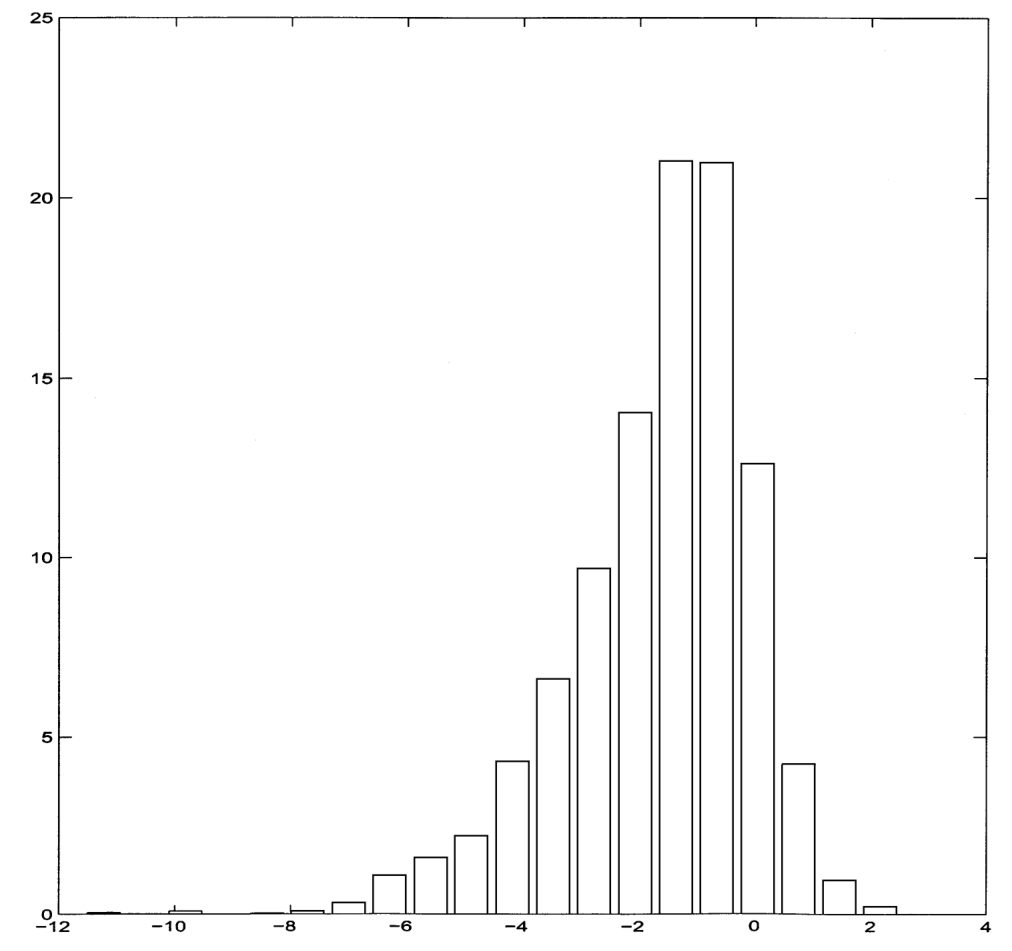
\includegraphics[width=\linewidth]{figures/ch08/nevo01_fig1_mushy.png}
\caption{Taste for sogginess (Mushy coefficient)}\label{fig:08-nevo-mushy}
\end{subfigure}\hfill
\begin{subfigure}[t]{0.48\linewidth}
\centering
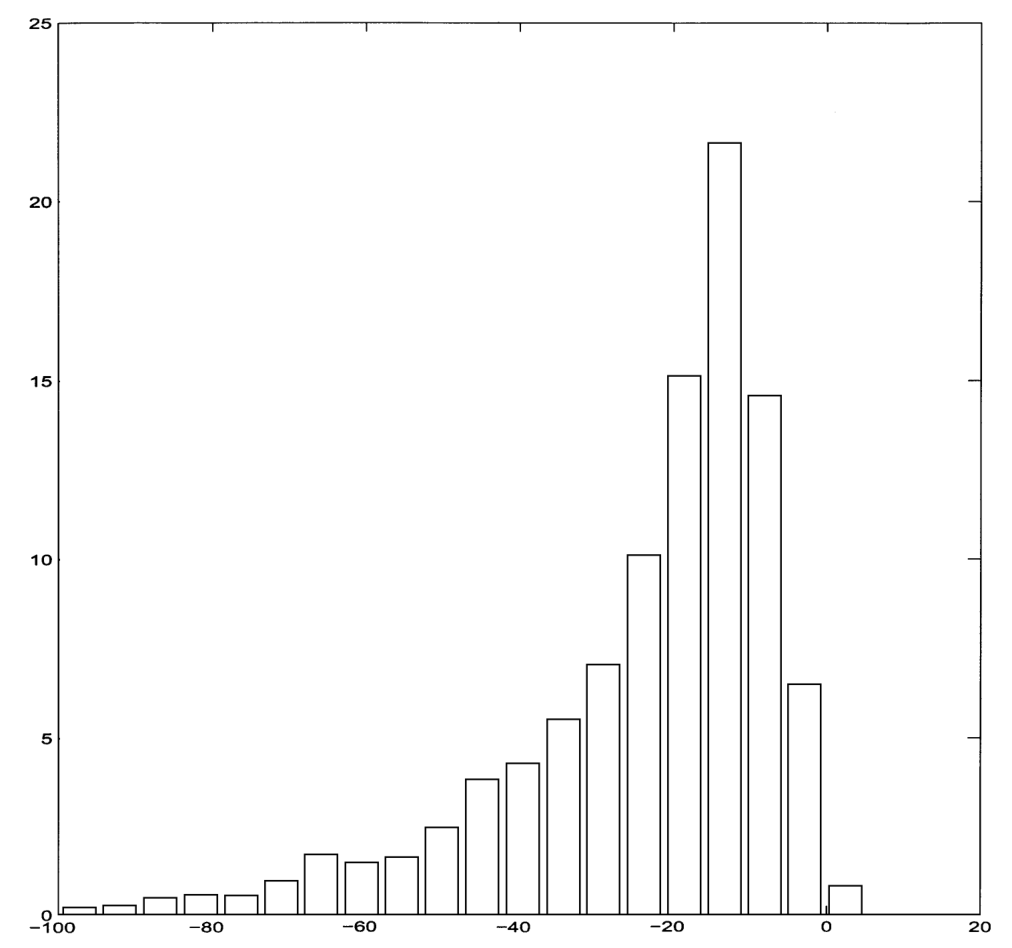
\includegraphics[width=\linewidth]{figures/ch08/nevo01_fig2_price.png}
\caption{Price coefficient}\label{fig:08-nevo-price}
\end{subfigure}
\caption{Frequency distributions of two individual coefficients implied by the estimates in
\cref{tab:08-nevo-full}. The horizontal axes give the value of the coefficient. The vertical axes, unlabeled
in the original, give frequencies. The bars sum to about 100, so the heights are percentages of simulated
consumers. Panel (a) puts about 15\% of consumers at a positive taste for sogginess. Panel (b) is skewed to the
left because it inherits the empirical distribution of demographics, and only 0.7\% of its mass lies above
zero.
Source: \citet{Nevo2001}, Figures 1 and 2.}
\label{fig:08-nevo-dists}
\end{figure}

The insignificance of the standard deviations says that the included demographics explain most of the
heterogeneity. The share of the variance of each coefficient explained by demographics exceeds 90\% (p.~330).
Appendix B of the paper re-estimates the model with the random shocks $\nu_i$ set to zero for the
characteristics that have demographic interactions. The estimates and margins barely change
(\cref{tab:08-nevo-robust}, column (i)). Nevo cautions against a stronger reading (p.~330, n.~26). The result
says that the data reject the assumed normal distribution for the unobserved part of tastes. It does not say
that information beyond demographics is useless. Purchase histories \citep{RossiMcCullochAllenby1996} and
second-choice data (the working-paper version of \citealp{BerryLevinsohnPakes2004}, \cref{sec:08-blp04}) do
reveal heterogeneity beyond demographics.

\casehead{Elasticities} \Cref{tab:08-nevo-elas} reproduces Table VII. Because elasticities vary across markets,
each entry is the median over the 1,124 markets of the elasticity of the row brand's share with respect to the
column brand's price. The own elasticities on the diagonal run from $-2.277$ (Cap'n Crunch) to $-4.252$
(Shredded Wheat). They are not ordered by price as the logit would require.

\begin{table}[htbp]
\centering
\caption{Median own- and cross-price elasticities of cereal demand}
\label{tab:08-nevo-elas}
\scriptsize
\setlength{\tabcolsep}{2.6pt}
\begin{tabular}{@{}rlrrrrrrrrrr@{}}
\toprule
 & & Corn & Frosted & Rice & Froot & & & Lucky & P Raisin & CapN & Shredded \\
\# & Brand & Flakes & Flakes & Krispies & Loops & Cheerios & Total & Charms & Bran & Crunch & Wheat \\
\midrule
1 & K Corn Flakes & $-$3.379 & 0.212 & 0.197 & 0.014 & 0.202 & 0.097 & 0.012 & 0.013 & 0.038 & 0.028 \\
2 & K Raisin Bran & 0.036 & 0.046 & 0.079 & 0.043 & 0.145 & 0.043 & 0.037 & 0.057 & 0.050 & 0.040 \\
3 & K Frosted Flakes & 0.151 & $-$3.137 & 0.105 & 0.069 & 0.129 & 0.079 & 0.061 & 0.013 & 0.138 & 0.023 \\
4 & K Rice Krispies & 0.195 & 0.144 & $-$3.231 & 0.031 & 0.241 & 0.087 & 0.026 & 0.031 & 0.055 & 0.046 \\
5 & K Frosted Mini Wheats & 0.014 & 0.024 & 0.052 & 0.043 & 0.105 & 0.028 & 0.038 & 0.054 & 0.045 & 0.033 \\
6 & K Froot Loops & 0.019 & 0.131 & 0.042 & $-$2.340 & 0.072 & 0.025 & 0.107 & 0.027 & 0.149 & 0.020 \\
7 & K Special K & 0.114 & 0.124 & 0.105 & 0.021 & 0.153 & 0.151 & 0.019 & 0.021 & 0.035 & 0.035 \\
8 & K Crispix & 0.077 & 0.086 & 0.114 & 0.034 & 0.181 & 0.085 & 0.030 & 0.037 & 0.048 & 0.043 \\
9 & K Corn Pops & 0.013 & 0.109 & 0.034 & 0.113 & 0.058 & 0.025 & 0.098 & 0.024 & 0.127 & 0.016 \\
10 & GM Cheerios & 0.127 & 0.111 & 0.152 & 0.034 & $-$3.663 & 0.085 & 0.030 & 0.037 & 0.056 & 0.050 \\
11 & GM Honey Nut Cheerios & 0.033 & 0.192 & 0.058 & 0.123 & 0.094 & 0.034 & 0.107 & 0.026 & 0.162 & 0.024 \\
12 & GM Wheaties & 0.242 & 0.169 & 0.175 & 0.025 & 0.240 & 0.113 & 0.021 & 0.026 & 0.050 & 0.043 \\
13 & GM Total & 0.096 & 0.108 & 0.087 & 0.018 & 0.131 & $-$2.889 & 0.017 & 0.017 & 0.029 & 0.029 \\
14 & GM Lucky Charms & 0.019 & 0.131 & 0.041 & 0.124 & 0.073 & 0.026 & $-$2.536 & 0.027 & 0.147 & 0.020 \\
15 & GM Trix & 0.012 & 0.103 & 0.031 & 0.109 & 0.056 & 0.026 & 0.096 & 0.024 & 0.123 & 0.016 \\
16 & GM Raisin Nut & 0.013 & 0.025 & 0.042 & 0.035 & 0.089 & 0.040 & 0.031 & 0.046 & 0.036 & 0.027 \\
17 & GM Cinnamon Toast Crunch & 0.026 & 0.164 & 0.049 & 0.119 & 0.089 & 0.035 & 0.102 & 0.026 & 0.151 & 0.022 \\
18 & GM Kix & 0.050 & 0.279 & 0.070 & 0.101 & 0.106 & 0.056 & 0.088 & 0.030 & 0.149 & 0.025 \\
19 & P Raisin Bran & 0.027 & 0.037 & 0.068 & 0.044 & 0.127 & 0.035 & 0.038 & $-$2.496 & 0.049 & 0.036 \\
20 & P Grape Nuts & 0.037 & 0.049 & 0.088 & 0.042 & 0.165 & 0.050 & 0.037 & 0.051 & 0.052 & 0.047 \\
21 & P Honey Bunches of Oats & 0.100 & 0.098 & 0.104 & 0.022 & 0.172 & 0.109 & 0.020 & 0.024 & 0.038 & 0.033 \\
22 & Q 100\% Natural & 0.013 & 0.021 & 0.046 & 0.042 & 0.103 & 0.029 & 0.036 & 0.052 & 0.046 & 0.029 \\
23 & Q Life & 0.077 & 0.328 & 0.091 & 0.114 & 0.137 & 0.046 & 0.096 & 0.023 & 0.182 & 0.029 \\
24 & Q CapN Crunch & 0.043 & 0.218 & 0.064 & 0.124 & 0.101 & 0.034 & 0.106 & 0.026 & $-$2.277 & 0.024 \\
25 & N Shredded Wheat & 0.076 & 0.082 & 0.124 & 0.037 & 0.210 & 0.076 & 0.034 & 0.044 & 0.054 & $-$4.252 \\
26 & Outside good & 0.141 & 0.078 & 0.084 & 0.022 & 0.104 & 0.041 & 0.018 & 0.021 & 0.033 & 0.021 \\
\bottomrule
\end{tabular}

\smallskip
\begin{minipage}{0.97\linewidth}
\footnotesize Notes: Entry $(i, j)$ is the percent change in the share of row brand $i$ for a one percent
change in the price of column brand $j$, as in \cref{eq:08-nevo-elas}. Each entry is the median over the 1,124
city-quarter markets. Own elasticities are negative numbers here, as in the paper. K, GM, P, Q and N denote
Kellogg, General Mills, Post, Quaker and Nabisco. Source: \citet{Nevo2001}, Table VII.
\end{minipage}
\end{table}

The substitution patterns follow characteristics. Lucky Charms, a children's cereal, is most sensitive to the
prices of other children's cereals (p.~330). It is least sensitive to the prices of Corn Flakes, Total and Wheaties, which
serve different segments.\footnote{Nevo names Corn Pops and Froot Loops as the brands to whose prices Lucky
Charms is most sensitive. Corn Pops and Wheaties are not among the ten columns printed in Table VII, so these
statements refer to the full matrix. Among the printed columns, row 14 is largest for Cap'n Crunch (0.147),
Frosted Flakes (0.131) and Froot Loops (0.124), and smallest for Corn Flakes (0.019).} The logit forces every
cross elasticity in a column to be equal. A summary of how far the estimates depart from that restriction is
the ratio of the largest to the smallest cross elasticity in a column, which equals one in the logit. The ratio
ranges from 21 for Corn Flakes to 3.5 for Shredded Wheat, with 95\% confidence intervals of 11 to 260 and 3
to 52 (p.~330). A low ratio also flags brands whose observed characteristics do not differentiate them well. A
formal test that all nonlinear parameters are zero, which is a specification test of the logit, is easily
rejected (p.~332, n.~28).

The last row gives the elasticity of the outside good's share with respect to each price. It is larger for
Corn Flakes (0.141) than for Froot Loops (0.022), in absolute terms and relative to the average cross elasticity
in each column (p.~332). Generic versions of Corn Flakes have larger shares than generic versions of Froot
Loops, and all generics belong to the outside good. A rise in the price of Corn Flakes therefore sends more
consumers to the outside option. Comparisons across columns should use semi-elasticities, because a one
percent price change differs in cents across brands (n.~29).

\subsection{Price-cost margins and the test of conduct}\label{sec:08-nevo01-margins}

\casehead{Predicted margins} \Cref{tab:08-nevo-margins} reproduces Table VIII and \cref{fig:08-nevo-margins}
plots it. Each entry is the median over the 27,862 observations of the margin implied by
\cref{eq:08-nevo-markup} under one ownership matrix. Medians are used to limit the influence of outliers, and
means with the 5\% tails trimmed are essentially identical (p.~332, n.~30). For the logit the computation is
analytical, using \eqref{eq:08-nevo-logit}. For the full model the confidence intervals come from 1,500
parametric bootstrap draws.

\begin{table}[htbp]
\centering
\caption{Median predicted price-cost margins under alternative conduct}
\label{tab:08-nevo-margins}
\footnotesize
\begin{tabular}{@{}lcc@{}}
\toprule
 & Logit & Full model \\
 & (\cref{tab:08-nevo-logit}, col.\ ix) & (\cref{tab:08-nevo-full}) \\
\midrule
Single-product firms & 33.6\% & 35.8\% \\
 & (31.8\%, 35.6\%) & (24.4\%, 46.4\%) \\
Current ownership of 25 brands & 35.8\% & 42.2\% \\
 & (33.9\%, 38.0\%) & (29.1\%, 55.8\%) \\
Joint ownership of 25 brands & 41.9\% & 72.6\% \\
 & (39.7\%, 44.4\%) & (62.2\%, 97.2\%) \\
Current ownership of all brands & 37.2\% & n.a. \\
 & (35.2\%, 39.4\%) & \\
Monopoly or perfect price collusion & 54.0\% & n.a. \\
 & (51.1\%, 57.3\%) & \\
\bottomrule
\end{tabular}

\smallskip
\begin{minipage}{0.84\linewidth}
\footnotesize Notes: Margins are $\frac{p - mc}{p}$, medians of the distribution over 27,862
brand-city-quarter observations. 95\% confidence intervals for the medians in parentheses, based on the
asymptotic distribution of the demand estimates. They are analytical for the logit and use 1,500 draws for the
full model. The last two rows require the shares of brands outside the sample, which suffice only for the
logit. Source: \citet{Nevo2001}, Table VIII.
\end{minipage}
\end{table}

\begin{figure}[htbp]
\centering
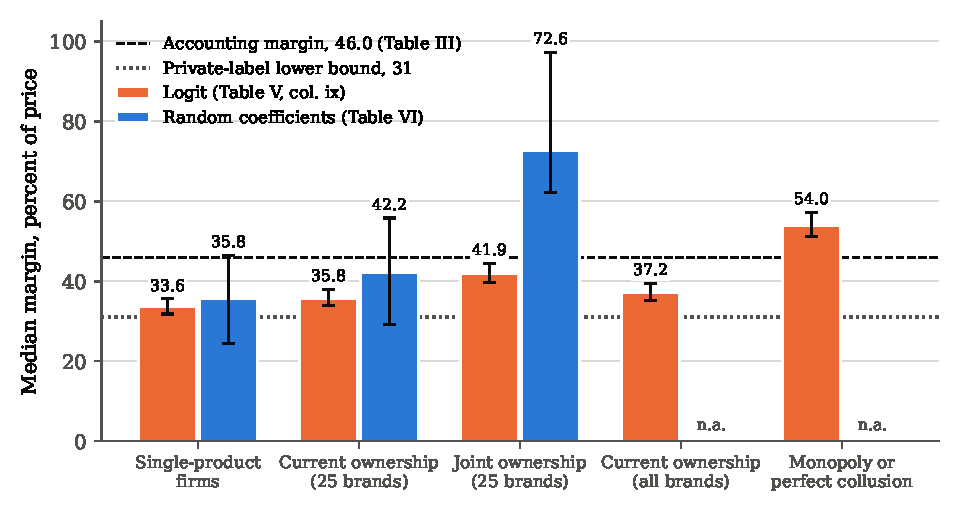
\includegraphics[width=0.97\linewidth]{figures/ch08/nevo01_margins.pdf}
\caption{Median predicted margins under five conduct models, with 95\% confidence intervals for the medians.
The dashed line is the accounting gross margin of 46.0\% of the retail price
(\cref{tab:08-nevo-costs}). The dotted line is the lower bound of about 31\% from the gap between national-brand
and private-label prices (p.~333). The random coefficients model predicts a joint-ownership margin far above
both lines, while its current-ownership interval covers them. The logit margins barely respond to ownership.
Redrawn from \citet{Nevo2001}, Table VIII.}
\label{fig:08-nevo-margins}
\end{figure}

The logit price coefficient, $-23.37$, is close to the full model's price coefficient in the Means column,
$-27.198$, yet their margins diverge as ownership widens. Under single-product pricing the medians are 33.6\% and 35.8\%. The portfolio effect adds 2.2
points in the logit and 6.4 points in the full model. Joint ownership of the 25 brands adds a further 6.1
points in the logit and 30.4 points in the full model. By \cref{prop:08-nevo-ownership}, these increments are
governed by the diversion ratios among co-owned brands. The full model concentrates diversion among similar
cereals, so joint pricing internalizes much more substitution.

The logit increments match \eqref{eq:08-nevo-logit} closely. In the logit the ratio of the joint-ownership
markup to the single-product markup of brand $j$ is $\frac{1-s_j}{1-S_{\mathcal{G}}}$. A rough calculation with
ratios of medians gives $\frac{41.9}{33.6} \approx 1.25$, which implies that the 25 brands hold about one fifth
of the potential market. Similarly $\frac{54.0}{33.6} \approx 1.61$ implies that all brands together hold
about 38\%. The ratio of the two, about one half, is consistent with the 43\% to 62\% of cereal volume that the
25 brands account for.\footnote{These are our calculations. A ratio of medians is not the median of the ratios,
and $s_j$ is treated as negligible, so the implied shares are approximations.}

\casehead{Observed margins} Testing requires a comparison with actual margins, which Nevo does not observe
directly. He treats the retail margin as an additional cost to manufacturers, which is consistent with many
models of manufacturer-retailer interaction (p.~333). The relevant observed margin is then the gross margin
relative to the retail price, 46.0\% from \cref{tab:08-nevo-costs}. This figure excludes promotional costs,
some of which, such as coupon rebates, are arguably marginal. Excluding them makes the observed margin a
generous one and the test conservative. Census data support the accounting figure. They are based on average
variable cost and give an upper bound.\footnote{The Census margin of 64.4\% is relative to the manufacturer's
price. On the retail-price basis of \cref{tab:08-nevo-costs}, Panel B, it corresponds to
$0.80 \times 64.4 \approx 51.5\%$. This conversion is ours.} A lower bound comes from the gap between the
prices of national brands and the corresponding private labels, about 31\% according to
\citet{Wongtrakool1994}. Private labels may carry a markup of their own and may have higher costs, so their
price exceeds the national brands' marginal cost and the gap understates the margin (pp.~333--334). Nevo
cautions that accounting margins are crude \citep{FisherMcGowan1983} and uses them only to discriminate
between models.

\casehead{The test} The predicted margins differ enough that even crude observed margins separate the models
(p.~334). The joint-ownership interval for the full model, 62.2\% to 97.2\%, lies above both the typical margin
of 46.0\% and the lower bound of 31\%. Joint profit maximization over the 25 brands is therefore rejected. The
current-ownership interval, 29.1\% to 55.8\%, contains both figures, so multi-product Nash-Bertrand pricing is
not rejected. The decomposition implied by the full model's medians attributes about 85\% of the
current-ownership margin to differentiation ($\frac{35.8}{42.2}$) and the remaining 6.4 points to the
portfolio effect.

Two further arguments strengthen the conclusion. The first concerns the restriction to 25 brands (p.~334). The
price coefficient should not be biased by the selection, and estimates on other samples confirm this. Brands
outside the sample are probably more elastic, which would lower the single-product margins. Weighting by
market shares, which is the likely effect of including small brands, offsets this. The share-weighted means
are roughly 2 to 3 points above the medians in Table VIII. For the current-ownership and collusive models a second force operates. Moving products from the
outside good into the inside set raises the predicted margins, and the effect grows with the number of jointly
priced products. Adding brands would therefore move the Nash-Bertrand prediction closer to the observed margins
and the collusive prediction further away. In this sense Table VIII is conservative.

The second argument concerns the logit. Applied to the logit column, the same test would not reject full
collusion over all products (p.~335). The logit's collusive margins, 41.9\% for the 25 brands and 54.0\% for
all brands, lie close to the observed margin of 46.0\%. Nevo stresses that this result is driven entirely by the logit's restrictive
substitution patterns and says nothing about conduct. It is the clearest demonstration in the paper of why
flexible substitution patterns matter for questions of market power.

\casehead{Why not a formal test} Nevo explains why he does not use two alternatives (pp.~334--335). One is to
estimate a conduct parameter, as in homogeneous-goods industries \citep{Bresnahan1989}. Its interpretation is
problematic \citep{Corts1999}, and its identification requirements are unlikely to be met with differentiated
products \citep{Nevo1998}. The other is a non-nested test of fully specified models
\citep{Bresnahan1987,GasmiLaffontVuong1992}. That requires the likelihood of each model, hence distributional
assumptions on the errors and a complete supply equation, and there is no natural set of such assumptions.
\Cref{ch:conduct} and \cref{sec:08-supply} discuss conduct testing more generally.

\subsection{Robustness*}\label{sec:08-nevo01-robust}

Appendix B of the paper reports four alternative specifications of the full model, reproduced in condensed form
in \cref{tab:08-nevo-robust}. Column (i) drops the random shocks $\nu_i$ for the characteristics that interact
with demographics. Its price coefficient ($-25.595$) and margins (36.1\%, 41.9\% and 67.4\%) are close to the
preferred ones, which supports the claim that demographics drive the heterogeneity. Columns (ii) and (iii) are
nonlinear least squares without instruments, without and with brand dummies. Their price coefficients are
$-4.291$ and $-7.407$. The implied margins are absurd. They range from 67.6\% to 84.5\% under Nash-Bertrand
pricing, and above 100\% under collusion. Column (iv) uses brand dummies as instruments, the analogue of
characteristic-based identification. Its estimates are imprecise and 22.4\% of its price coefficients are
positive. Nevo notes that it lacks the variance-reduction methods of BLP (p.~339).

\begin{table}[htbp]
\centering
\caption{Alternative specifications of the full model}
\label{tab:08-nevo-robust}
\footnotesize
\begin{tabular}{@{}lrrrr@{}}
\toprule
 & (i) & (ii) & (iii) & (iv) \\
 & No $\nu_i$ on & NLLS, no & NLLS, brand & GMM, brand \\
 & interacted chars. & brand dummies & dummies & dummies as IVs \\
\midrule
Mean price coefficient & $-$25.595 & $-$4.291 & $-$7.407 & $-$9.856 \\
 & (2.673) & (0.143) & (0.164) & (3.039) \\
Price $\times$ income & 311.101 & 34.565 & 8.552 & 21.575 \\
 & (61.797) & (1.455) & (0.974) & (96.912) \\
Percent of price coefficients $>0$ & 0 & 16.1 & 0 & 22.4 \\
\addlinespace
Single-product margin & 36.1\% & 67.6\% & 75.7\% & 48.2\% \\
Multi-product margin & 41.9\% & 75.6\% & 84.5\% & 54.0\% \\
Collusive margin & 67.4\% & 103.9\% & 117.6\% & 88.9\% \\
\bottomrule
\end{tabular}

\smallskip
\begin{minipage}{0.88\linewidth}
\footnotesize Notes: Standard errors in parentheses. 27,862 observations. NLLS is nonlinear least squares,
which does not instrument for price. Column (i) is the preferred specification without $\nu_i$ for the
characteristics that have demographic interactions. The paper also reports all taste parameters, omitted here.
The preferred specification gives 35.8\%, 42.2\% and 72.6\% (\cref{tab:08-nevo-margins}). Source:
\citet{Nevo2001}, Table B(II).
\end{minipage}
\end{table}

Other checks point the same way (pp.~327, 335--336). A specification with city fixed effects, the analogue of
column (x) of \cref{tab:08-nevo-logit}, gives point estimates close to the preferred ones but very large
standard errors. This is expected, since demographics barely change within a city over five years. A
multi-stage budgeting demand system in the style of \citet{HausmanLeonardZona1994} and \citet{Hausman1997},
covered in \cref{ch:aids}, shows interesting differences in cross-price substitution but the same conclusions
about conduct. Studies based on household data, a random coefficients model by \citet{Kiser1996} and a nested
logit by \citet{Shum1999}, use different data and different identifying assumptions. They produce very similar
own- and cross-price elasticities.

\subsection{Interpretation, limitations and contribution}\label{sec:08-nevo01-assess}

\casehead{Interpretation} If Nash-Bertrand pricing is the benchmark of noncollusive behavior, prices in RTE
cereal are not collusive, even with margins above 45\% (p.~336). High margins reflect consumers' willingness
to pay for their favorite brands and firms' internalization of substitution within their portfolios. To the
extent that the industry has market power, it lies in the ability to maintain a portfolio of differentiated
brands and to shape perceived quality through advertising. Nevo relates this to the FTC case. The standard
account of the complaint mentions cooperative pricing, but its core was brand proliferation as a barrier to
entry \citep{Schmalensee1978}. In this sense the FTC focused on the dimensions of competition that Nevo finds
important. His model, however, takes brands and advertising as given and cannot evaluate their competitive
effects (p.~336).

\casehead{Limitations} The test rules out only the extreme form of cooperation, joint maximization of profits
over all 25 brands. Cooperation within a subset of products or firms, such as two raisin brans or two smaller
producers, is not tested and would require more detailed cost data (p.~336). The observed margin is a single
accounting figure for a typical Kellogg brand, compared with medians over brands, cities and quarters. The
Hausman instruments rest on independence of demand shocks across cities, which overidentification tests reject
in the logit unless city effects are added. Advertising is treated as exogenous, and its implied elasticity is
implausibly low. The model is static and uses quarterly averages of prices that include temporary promotions.
The standard deviations of the random coefficients are imprecise because the choice set barely varies. The
full model's margins have wide confidence intervals. The single-product interval runs from 24.4\% to 46.4\%.
Finally, the definition of the potential market as one serving per person per day fixes the outside share,
and with it the level of the implied markups (\cref{sec:08-model}).

\casehead{Contribution} The paper made four contributions that became standard. It combined brand fixed effects
with the BLP estimator and recovered taste means by minimum distance, so that price endogeneity due to $\xi_j$
needs no instrument. It used prices in other markets as instruments in a random coefficients model and checked
them against cost proxies. It modeled heterogeneity with the empirical distribution of demographics. Above all,
it turned the supply side into a tool for measuring conduct. Comparing margins implied by alternative ownership
matrices with observed margins gives a transparent decomposition of market power. The same model and data
underlie the merger simulations of \citet{Nevo2000b}, discussed in \cref{ch:mergers}. Hausman's valuation of a
new cereal brand, discussed in \cref{ch:newgoods}, depends on the same kind of assumption about price
competition that Nevo tests. Later work uses the demand elasticities to discriminate between models of conduct
in the same industry, including common-ownership pricing \citep{BackusConlonSinkinson2021}.

\begin{table}[htbp]
\centering
\caption{Identification and counterfactual map of Nevo (2001)}
\label{tab:08-nevo01-map}
\footnotesize
\renewcommand{\arraystretch}{1.1}
\begin{tabularx}{\textwidth}{@{}>{\raggedright\arraybackslash}p{2.6cm}>{\raggedright\arraybackslash}X@{}}
\toprule
Observed data & IRI scanner prices and servings of 25 cereal brands in up to 65 cities, quarterly from 1988 to
  1992 (27,862 brand-city-quarters). Brand characteristics, national advertising, CPS demographic draws, and
  accounting margins for a typical brand. \\
\addlinespace
Latent objects & City-quarter quality deviations $\tilde\xi_{jt}$, consumer tastes $\nu_i$, marginal costs
  and markups. \\
\addlinespace
Estimated parameters & The price and advertising coefficients, brand and quarter effects, demographic
  interactions $\Pi$ and standard deviations $\Sigma$. Taste means come from a minimum-distance step. \\
\addlinespace
Identifying variation & Prices of the same brand in other cities of the region, checked against cost
  proxies. Brand effects absorb national quality, and cross-city differences in demographics identify $\Pi$. \\
\addlinespace
Maintained assumptions & City demand shocks are independent across cities after brand, time and demographic
  controls, and costs share a regional component. Static pricing, exogenous advertising, and a potential
  market of one serving per person per day. \\
\addlinespace
Counterfactual and what it holds fixed & Margins implied by \eqref{eq:08-nevo-markup} under single-product,
  current and joint ownership, at observed prices and shares. Demand is held at its estimates, and only the
  ownership matrix changes. \\
\addlinespace
Conclusion & Current ownership predicts a median margin of 42.2 percent, whose interval contains the
  observed margins. Joint ownership of the 25 brands predicts 72.6 percent and is rejected. Margins come
  from differentiation and portfolios, given the Hausman instruments. \\
\addlinespace
One limitation & Only joint profit maximization over all 25 brands is tested. Collusion within a subset of
  brands or firms is not. \\
\addlinespace
Source and our additions & The tables are Nevo's. \Cref{prop:08-nevo-ownership}, the advertising
  benchmark and the logit share calculations behind the margin ratios are ours. \\
\addlinespace
Tools in the appendices & \Cref{sec:A-iv,sec:A-gmm,sec:A-delta-boot}. \\
\bottomrule
\end{tabularx}
\end{table}

\section{Case study: Berry, Levinsohn and Pakes (2004), micro and macro data}\label{sec:08-blp04}

\citet{BerryLevinsohnPakes2004}, henceforth BLP (2004), return to the automobile market with a new kind of
data. A proprietary survey by General Motors covers a large sample of 1993 new-vehicle buyers. It records
each buyer's demographics, the vehicle bought and the vehicle the buyer would have bought had the first choice
been unavailable. The paper asks what such consumer-level data, and second choices in particular, add to the
identification of substitution patterns. The answer has three parts. Second choices pin down the parameters
that govern substitution. Unobserved heterogeneity in tastes is needed to match them, even with rich
demographics. A single cross section still cannot determine the level of price elasticities. The general
estimator was introduced in \cref{sec:08-micro}. Here we follow the paper in detail, and
\cref{tab:08-blp04-map} at the end of the section maps it. Page numbers refer to the
journal article.\footnote{BLP (2004) write observed household attributes as $z_{ir}$, the coefficients on
their interactions with characteristics as $\beta^{o}_{kr}$ (``observed'') and the standard deviations of
unobserved tastes as $\beta^{u}_k$ (``unobserved''). We write $D_{ir}$, $\pi_{kr}$ and $\sigma_k$, so that
$\beta^{o}$ and $\beta^{u}$ correspond to the matrices $\Pi$ and $\Sigma$ of \cref{sec:08-model}.}

\subsection{The question}\label{sec:08-blp04-question}

We abbreviate \citet{BerryLevinsohnPakes1995}, the subject of \cref{sec:08-blp95}, as BLP (1995). In that
paper, substitution patterns are identified from changes across markets and years in the choice set and in the
distribution of consumer attributes. The distribution of tastes,
conditional on observed incomes, is assumed to be stable over time (pp.~69--70). Earlier discrete choice work,
and \citet{Goldberg1995} and \citet{Petrin2002} in industrial organization, matched consumer attributes to
choices. Such data identify substitution to the extent that observed attributes explain it.
\Cref{sec:08-goldberg} discusses Goldberg's study.

Second-choice data offer a different source of identification (p.~70). They give a direct, data-based measure
of substitution, so one can ask which models reproduce it. By requiring the parameters to match observed
second choices, the econometrician gains identifying power that does not rely on exogenous changes in choice
sets. The paper also stresses a limit. Second choices in a single cross section, with one price per vehicle,
reveal the pattern of substitution but not the level of price elasticities. Outside information must fix the
level. The paper closes with two out-of-sample predictions, the introduction of luxury sport utility vehicles
and the closure of the Oldsmobile division of General Motors.

\subsection{Data}\label{sec:08-blp04-data}

\casehead{The CAMIP survey} The consumer data come from a proprietary survey conducted for General Motors,
here called CAMIP (pp.~79--80). It samples from the registrations of 1993 model-year vehicles of all
manufacturers, not only GM. For each vehicle a given number of buyers is sampled, so the design is a random
sample conditional on the vehicle purchased. A sample of this kind is called \emph{choice-based}. The subsample
used has 37,500 observations. The questionnaire asks about income, age of the household head, family size and
place of residence, and each question is matched to a question in the CPS.

\Cref{tab:08-blp04-samples} compares CAMIP households with CPS households. CAMIP over-represents high incomes.
Only 6.52\% of CPS households earn \$85,000 or more, against 25.13\% of CAMIP households, and mean income is
\$72,270 in CAMIP against \$34,170 in the CPS. New-vehicle buyers are richer than the population. More
surprisingly, CAMIP households are less urban (35\% against 46\%) and more rural (35\% against 25\%).
Rural households buy a disproportionate number of vehicles, which helps explain the high share of trucks
(p.~80).

\begin{table}[htbp]
\centering
\caption{CPS and CAMIP household samples}
\label{tab:08-blp04-samples}
\footnotesize
\begin{tabular}{@{}lrrrr@{}}
\toprule
Income range (\$) & Percent in CPS & Percent in CAMIP & CPS group mean & CAMIP group mean \\
\midrule
0--36,500 & 64.17 & 25.00 & 16.90 & 25.96 \\
36,500--55,000 & 16.97 & 23.16 & 44.89 & 45.43 \\
55,000--85,000 & 12.34 & 26.71 & 66.93 & 67.46 \\
85,000 and above & 6.52 & 25.13 & 114.25 & 148.19 \\
All & 100.00 & 100.00 & 34.17 & 72.27 \\
\midrule
Other demographics & & & CPS mean & CAMIP mean \\
\midrule
Family size & & & 2.36 & 2.65 \\
Age of household head & & & 46.80 & 46.18 \\
Number of kids & & & 0.66 & 0.58 \\
Urban & & & 0.46 & 0.35 \\
Rural & & & 0.25 & 0.35 \\
Suburban & & & 0.29 & 0.30 \\
\bottomrule
\end{tabular}

\smallskip
\begin{minipage}{0.86\linewidth}
\footnotesize Notes: Group means of income in thousands of dollars. Source:
\citet{BerryLevinsohnPakes2004}, Table 1.
\end{minipage}
\end{table}

\casehead{The choice set and product data} The vehicle list follows GM's sampling cells and has 203 vehicles:
147 cars, 25 sport utility vehicles (SUVs), 17 vans and 14 pickup trucks (p.~81). Early runs used 218
vehicles. The final runs aggregate 15 very expensive vehicles, with an average price of \$74,000 and a combined
share of 0.3\% of vehicles sold, into one ``super-luxury'' model (n.~9). The survey records transaction prices.
Characteristics are those of the modal vehicle in each cell, the most commonly purchased combination of
options, and price is the average price of that modal vehicle. About 10.6 million vehicles were sold in 1993
at an average price of \$18,500, for total sales of about \$196 billion. The continuous characteristics are horsepower
per weight (HP), number of passengers (Pass, a measure of size), city miles per gallon (MPG) and number of power
accessories (Acc). They also include safety features (Safe, antilock brakes plus airbags) and the payload of
light trucks. The
dummies mark minivans, SUVs, pickups, full-size vans, sports cars and four- or all-wheel drive (Allw). The interactions
PUPayl and SUVPayl multiply payload by the pickup and SUV dummies (Table 2).

\casehead{Demographic patterns} Means of vehicle characteristics by demographic group reveal clear interactions
(p.~81). Examples are kids with minivans, income with price, rural residence with pickups and four-wheel drive,
and age with nearly everything. The authors used such tables to choose the interactions in utility.
\Cref{tab:08-blp04-groups} condenses their Table 4. The mean price of the vehicle chosen rises from \$16,600 in
the lowest income group to \$26,300 in the highest. Households with two or more children choose a minivan 18\% of
the time, against 3\% for households without children. The mean of PUPayl, the pickup dummy times payload in
thousands of pounds, is 0.31 among rural households, against 0.14 among urban and 0.10 among suburban households. Buyers over 50 choose vehicles that are more
expensive and larger, with more accessories, and they rarely choose sports cars or SUVs (0.07 and 0.04).

\begin{table}[htbp]
\centering
\caption{Mean characteristics of the vehicles chosen by demographic group in the CAMIP data (condensed)}
\label{tab:08-blp04-groups}
\footnotesize
\setlength{\tabcolsep}{4.5pt}
\begin{tabular}{@{}lrrrrrrrrrr@{}}
\toprule
Group & Price & HP & Pass & Acc & Sport & MPG & Allw & Miniv & SUV & PUPayl \\
\midrule
\multicolumn{11}{@{}l}{\textit{Age of household head}} \\
\quad 30 or less & 16.6 & 4.7 & 4.5 & 2.6 & 0.20 & 22.0 & 0.13 & 0.03 & 0.15 & 0.24 \\
\quad 30--50 & 20.1 & 4.8 & 4.9 & 3.1 & 0.15 & 20.4 & 0.13 & 0.08 & 0.13 & 0.18 \\
\quad Over 50 & 22.4 & 4.9 & 5.1 & 3.4 & 0.07 & 19.8 & 0.06 & 0.04 & 0.04 & 0.19 \\
\multicolumn{11}{@{}l}{\textit{Number of children}} \\
\quad 0 & 20.9 & 4.9 & 4.8 & 3.2 & 0.14 & 20.4 & 0.10 & 0.03 & 0.09 & 0.20 \\
\quad 1 & 19.2 & 4.7 & 4.8 & 3.0 & 0.13 & 21.0 & 0.12 & 0.06 & 0.11 & 0.20 \\
\quad 2 or more & 20.1 & 4.6 & 5.3 & 3.1 & 0.08 & 19.9 & 0.12 & 0.18 & 0.13 & 0.16 \\
\multicolumn{11}{@{}l}{\textit{Residence}} \\
\quad Urban & 20.6 & 4.8 & 4.9 & 3.2 & 0.13 & 20.7 & 0.10 & 0.05 & 0.10 & 0.14 \\
\quad Suburban & 21.7 & 5.0 & 4.9 & 3.4 & 0.15 & 20.3 & 0.10 & 0.06 & 0.10 & 0.10 \\
\quad Rural & 19.2 & 4.7 & 4.9 & 3.0 & 0.11 & 20.2 & 0.12 & 0.06 & 0.11 & 0.31 \\
\multicolumn{11}{@{}l}{\textit{Household income (\$)}} \\
\quad 37,000 or less & 16.6 & 4.6 & 4.8 & 2.6 & 0.12 & 21.9 & 0.08 & 0.04 & 0.07 & 0.25 \\
\quad 37,000--55,000 & 18.5 & 4.7 & 4.9 & 3.0 & 0.12 & 20.7 & 0.10 & 0.07 & 0.10 & 0.24 \\
\quad 55,000--85,000 & 20.3 & 4.8 & 4.9 & 3.2 & 0.14 & 20.0 & 0.13 & 0.07 & 0.13 & 0.19 \\
\quad Over 85,000 & 26.3 & 5.2 & 4.9 & 3.7 & 0.14 & 19.1 & 0.11 & 0.05 & 0.12 & 0.08 \\
\bottomrule
\end{tabular}

\smallskip
\begin{minipage}{0.95\linewidth}
\footnotesize Notes: Price in thousands of dollars. Sport, Allw, Miniv and SUV are shares of vehicles with the
attribute. PUPayl is the pickup dummy times payload in thousands of pounds. The original table also reports
safety features, the van dummy, SUV payload and rows by family size. Source: \citet{BerryLevinsohnPakes2004},
Table 4 (p.~84).
\end{minipage}
\end{table}

\casehead{Second choices}
\Cref{tab:08-blp04-second} reproduces the second-choice information for 17 representative vehicles. The 166
sampled buyers of the Ford Escort named the Ford Tempo most often (16 buyers), followed by the Ford Taurus.
Together these two account for 18\% of Escort buyers, who named 53 different second choices in all (p.~86).
Second choices are more concentrated for light trucks and expensive cars. They are often made by the same
company as the first choice, which supports pricing that maximizes the joint profits of each firm's products.

\begin{table}[htbp]
\centering
\caption{Examples of second choices in the CAMIP data}
\label{tab:08-blp04-second}
\footnotesize
\setlength{\tabcolsep}{4pt}
\begin{tabular}{@{}lrlrlrr@{}}
\toprule
 & & Modal second & Number & Next second & (Modal $+$ & Different \\
First choice & $n_j$ & choice & choosing & choice & next)$\,\div\, n_j$ & choices \\
\midrule
Metro & 188 & Escort & 22 & Geo Storm & .22 & 49 \\
Cavalier & 238 & Escort & 16 & LeBaron & .12 & 59 \\
Escort & 166 & Tempo & 16 & Taurus & .18 & 53 \\
Corolla & 250 & Civic & 42 & Camry & .33 & 55 \\
Sentra & 203 & Corolla & 34 & Civic & .31 & 60 \\
Accord & 223 & Camry & 58 & Taurus & .35 & 61 \\
Taurus & 147 & Camry & 18 & Sable & .22 & 45 \\
Legend & 119 & Lexus ES300 & 19 & Lexus SC300 & .24 & 40 \\
Seville & 243 & DeVille & 38 & Lincoln MK8 & .26 & 49 \\
Lexus LS400 & 148 & DeVille & 33 & Infiniti Q45 & .39 & 27 \\
Caravan & 166 & Voyager & 31 & Aerostar & .32 & 36 \\
Quest & 232 & Caravan & 50 & Villager & .43 & 31 \\
Grand Cherokee & 137 & Explorer & 75 & Blazer & .59 & 34 \\
Trooper & 137 & Explorer & 43 & Rodeo & .41 & 27 \\
GMC full-size pickup & 469 & Chevy full-size pickup & 222 & Ford full-size pickup & .55 & 29 \\
Toyota pickup & 113 & Ford Ranger & 29 & Nissan pickup & .43 & 25 \\
Econovan & 90 & Chevy full-size van & 20 & Suburban & .44 & 23 \\
\bottomrule
\end{tabular}

\smallskip
\begin{minipage}{0.92\linewidth}
\footnotesize Notes: $n_j$ is the number of CAMIP buyers of the first-choice vehicle. The sixth column is the
fraction of them whose second choice is either the modal or the next most common second choice. Source:
\citet{BerryLevinsohnPakes2004}, Table 5.
\end{minipage}
\end{table}

Second choices resemble first choices. Across households, the correlations between the characteristics of the
first and the second choice are all positive and highly significant (p.~86). They are about 0.7 for price and
the minivan dummy, about 0.6 for MPG, size and the other type dummies, and between 0.3 and 0.5 for the rest.
The survey does not ask whether the household would have bought a vehicle at all. The data therefore say
nothing directly about substitution to the outside good.

\subsection{The model}\label{sec:08-blp04-model}

Households $i$ choose among vehicles $j = 1,\dots,J$ and the outside option $j = 0$. Let $k$ index observed
characteristics, including price, and $r$ index observed household attributes. Utility is linear in
characteristics (BLP 2004, equations (1) and (2)):
\begin{equation}\label{eq:08-blp04-utility}
u_{ij} = \sum_k x_{jk}\beta_{ik} + \xi_j + \epsilon_{ij},
\qquad
\beta_{ik} = \bar\beta_k + \sum_r D_{ir}\pi_{kr} + \sigma_k\nu_{ik} .
\end{equation}
The idiosyncratic shocks $\epsilon_{ij}$ are i.i.d.\ type-I extreme value, and the $\nu_{ik}$ are independent
standard normals. Substituting the taste equation into utility gives (equations (3) and (4))
\begin{equation}\label{eq:08-blp04-delta}
u_{ij} = \delta_j + \sum_{k,r} x_{jk}D_{ir}\pi_{kr} + \sum_k x_{jk}\nu_{ik}\sigma_k + \epsilon_{ij},
\qquad
\delta_j = \sum_k x_{jk}\bar\beta_k + \xi_j .
\end{equation}
The model has one unobserved product characteristic, valued equally by all households. The authors note that
this simplifies computation but is not essential to their arguments (p.~71, n.~3).

\casehead{Price and income} Price receives special treatment (p.~87). The household-specific part of the
price coefficient is $-e^{-W_i}$, where $W_i$ is ``effective wealth,''
\begin{equation}\label{eq:08-blp04-wealth}
W_i = \sum_r D_{ir}\pi_{wr} + \sigma_w\nu_{iw} .
\end{equation}
The common part of the price coefficient, $\bar\beta_p$, sits in $\delta_j$ by \cref{eq:08-blp04-delta}.
Write $\bar\alpha = -\bar\beta_p$. Household $i$'s price sensitivity is then
\begin{equation}\label{eq:08-blp04-alpha}
\alpha_i = \bar\alpha + e^{-W_i}.
\end{equation}
Because $e^{-W_i} > 0$, no household with $\bar\alpha \geq 0$ prefers higher prices, which is the reason for the
exponential form. The factor $e^{-W_i}$ is lognormal given demographics. The attributes in $W_i$ are a constant,
family size and a spline in income. Preliminary runs allowed the slope of the spline to change at each quartile
of the CAMIP income distribution, but only a change at the 75th percentile was needed. Higher income raises
$W_i$ and lowers price sensitivity.

\casehead{The outside good} Little is known a priori about the value of not buying. Early runs let it depend
linearly on all household attributes plus a normal disturbance. Only income, family size and sometimes the
number of adults mattered (p.~87). The normal disturbance on the outside good plays the role of a random
coefficient on the inside-good constant (\cref{sec:08-model}).

\casehead{What micro data identify} Equation \eqref{eq:08-blp04-delta} is a random coefficients discrete
choice model with a separate constant $\delta_j$ for each product. Given parametric assumptions on
$(\nu,\epsilon)$, the micro data identify $(\delta, \Pi, \Sigma)$ without any assumption on the joint
distribution of $(\xi, x)$ (pp.~72--73). Some questions, such as ideal price indices, need only these
parameters. Elasticities, however, also require the effect of price on $\delta_j$, that is, $\bar\beta_p$. The
equation $\delta_j = \sum_k x_{jk}\bar\beta_k + \xi_j$ has only $J$ observations, and price is correlated with
$\xi_j$. Identifying $\bar\beta$ therefore requires an assumption on $(\xi, x)$, the same identification
problem as in BLP (1995). Micro data solve one part of the problem, the substitution parameters, and leave the
other part untouched. \citet{BerryHaile2024}, discussed in \cref{sec:08-micro}, generalize this division of
labor nonparametrically.

Aggregate demand integrates over the distribution $P_w$ of household attributes $w_i = (D_i, \nu_i,
\epsilon_i)$ (equation (5)):
\[
s_j(\delta, \Pi, \Sigma; x, P_w) = \int_{A_j(\delta, \Pi, \Sigma; x)} P_w(\dd w),
\qquad A_j = \Big\{w : \max_{r = 0,\dots,J} u_{ir}(w) = u_{ij}\Big\}.
\]
Conditional on $(D_i, \nu_i)$, the logit form gives the choice probability (equation (6))
\begin{equation}\label{eq:08-blp04-prob}
\Pr(j^{(1)}_i = j \mid D_i, \nu_i, \theta) =
\frac{\exp\big(\delta_j + \sum_{k,r}x_{jk}D_{ir}\pi_{kr} + \sum_k x_{jk}\nu_{ik}\sigma_k\big)}
{1 + \sum_q \exp\big(\delta_q + \sum_{k,r}x_{qk}D_{ir}\pi_{kr} + \sum_k x_{qk}\nu_{ik}\sigma_k\big)},
\end{equation}
where $\theta = (\delta, \Pi, \Sigma)$ and $j^{(1)}_i$ denotes household $i$'s first choice.

\subsection{The estimator}\label{sec:08-blp04-estimator}

Maximum likelihood is efficient but was too burdensome, so the authors use a method of moments estimator
(p.~74). It matches three sets of moments (p.~75).
\begin{enumerate}
\item \emph{First-choice moments.} Covariances between the characteristics of the vehicle bought and the
attributes of the household, for example family size and vehicle size. They identify $\Pi$. The means of
household attributes among buyers identify the parameters of the outside good, because CAMIP samples vehicles
roughly in proportion to their shares.
\item \emph{Second-choice moments.} Covariances between the characteristics of the first and the second
choice, one for each characteristic with a random coefficient. They identify $\Sigma$. If $\Sigma = 0$, the
observed attributes alone determine both choices and hence their correlation. A predicted correlation far below
the observed one signals that unobserved tastes matter.
\item \emph{Market shares} of the $J$ products, which identify $\delta$.
\end{enumerate}
A footnote makes the role of interactions precise (p.~75, n.~5). If $\Pi = 0$ and only first choices were
used, aggregate shares would be sufficient statistics for the first-choice data. Matching individuals to their
vehicles would then add no information.

\casehead{Concentrating out the product constants} With over 200 vehicles, $\delta$ has over 200 elements and
the full parameter vector about 250 (p.~77). The authors exploit the precision of the aggregate shares. The
observed share vector $s^N$, computed from $N$ households (over 100 million), is multinomial around the true
$s(\delta_0, \beta_0)$ with variance of order $N^{-1}$. An efficient estimator therefore sets predicted shares
equal to observed shares. Let $\theta_2 = (\Pi, \Sigma)$, which BLP (2004) call $\beta$. For each trial value of
$\theta_2$, the contraction of \cref{sec:08-inversion} finds the $\delta^{n_s,N}(\theta_2)$ that solves the simulated
share equations \eqref{eq:08-blp04-shares} (their equation (7)). The pairs $(D_r, \nu_r)$ combine a CPS draw of
demographics with a draw of $\nu$. They are drawn once and held fixed, as \citet{PakesPollard1989} require. Importance
sampling as in BLP (1995) reduces simulation variance (p.~77, n.~6). The micro moments are then evaluated at
$(\theta_2, \delta^{n_s,N}(\theta_2))$, and the search runs over $\theta_2$ alone.

\casehead{First-choice moments and Bayes' rule} Because the sample is choice-based, the model's prediction to
be matched is the expected attribute of a household that chose a given vehicle. Let $n_j$ be the number of
sampled buyers of $j$ and $n = \sum_j n_j$. The first-choice moments \eqref{eq:08-blp04-g1} (their equation (8))
compare the sample mean attribute of $j$'s buyers with its model counterpart, one moment for each interaction in
utility. The model counterpart is the Bayes formula \eqref{eq:08-bayes} (their equation (9)). By construction of
$\delta^{n_s,N}(\theta_2)$, its denominator equals $s^N_j$, and its numerator is simulated with the same draws as the
shares, as in \eqref{eq:08-bayes-sim} (their equation (10)). The approach follows the literature on choice-based
sampling \citep{ManskiLerman1977,ImbensLancaster1994}. The same structure underlies the micro moments of
\citet{Petrin2002} in \cref{ch:newgoods}.

\casehead{Second-choice probabilities} The second-choice moments require the probability that a household
whose first choice is $j$ names $q$ as its second choice. The survey asks for a second vehicle, so both $j$
and the outside good leave the choice set. By \cref{lem:08-blp04-second}, conditional on $(D_i, \nu_i)$ the
probability is again a logit with $j$ and the outside good removed from the denominator (p.~79). It equals
$\Pr(j^{(2)}_i = q \mid j^{(1)}_i = j, D_i, \nu_i, \theta_2) = \frac{\exp(V_{iq})}{\sum_{l \neq 0, j}\exp(V_{il})}$,
where $V_{il}$ is the deterministic utility in \eqref{eq:08-blp04-prob}. The individual second choice satisfies IIA, but
the aggregate one does not, because the integral over $(D,\nu)$ weights each household by its probability of having
chosen $j$ first, as in \eqref{eq:08-second-agg}. Buyers of $j$ have tastes favorable to $j$'s characteristics and pick
second choices with similar characteristics. The second-choice moment for characteristic $k$ starts from the average
$x_k$ of the second choices named by $j$'s buyers. It subtracts the model's prediction, interacts the difference with
$x_{kj}$ and averages over $j$ with weights $\frac{n_j}{n}$ (their equations (11) and (12)). The prediction is
\[
\E\Big[\sum_{q\neq j} x_{qk}\,\indic\{j^{(2)} = q\} \Bigm| j^{(1)} = j, \theta_2\Big]
= \frac{\int\!\int \sum_{q \neq j} x_{qk}\Pr(q \mid j, D, \nu, \theta_2)\,\Pr(j \mid D,\nu,\theta_2)\,P(\dd D,\dd\nu)}
{s_j^N},
\]
where the posterior weighting mirrors \eqref{eq:08-bayes}. It is simulated with the same draws.

\casehead{GMM and inference} The moments $G^1$ and $G^2$ are stacked, and $\theta_2$ is estimated by two-step GMM
\citep{Hansen1982}. The estimator is consistent if $n_s \to \infty$ and $N \to \infty$ as $n \to \infty$
(p.~79). Since $N$ is much larger than $n$ and $n_s$, the authors use the limit distribution with
$\frac{N}{n} \to \infty$ and $\frac{n_s}{n}$ converging to a positive constant. The asymptotic variance then
includes simulation error. The variance of the moments is the sum of a sampling part (from the CAMIP means) and
a simulation part (from the draws), since the two errors are independent (Appendix, p.~103). The simulation
part is estimated by recomputing the moments, including a new solution of \eqref{eq:08-blp04-shares}, for many
independent sets of draws. The derivative of the moments has two terms, a direct effect of $\theta_2$ and an
effect through $\delta(\theta_2)$. Typically somewhat less than half of the variance of the estimates comes from
simulation (p.~90, n.~15).

\subsection{Estimates of the interaction parameters}\label{sec:08-blp04-estimates}

\Cref{tab:08-blp04-pi} reproduces Table 6, the estimates of $\Pi$, and \cref{tab:08-blp04-sigma} reproduces
Table 7, the estimates of $\Sigma$. Each table compares the full model with restricted models. Two are logits
with $\Sigma = 0$ but with product constants and observed interactions, estimated from first choices only and
from first and second choices. The third sets $\Pi = 0$, like BLP (1995), and appears only in Table 7
(p.~87).

\begin{table}[htbp]
\centering
\caption{Estimates of the interactions with observed household attributes ($\Pi$)}
\label{tab:08-blp04-pi}
\footnotesize
\begin{tabular}{@{}llrrr@{}}
\toprule
 & & & \multicolumn{2}{c}{Logit ($\Sigma = 0$)} \\
\cmidrule(l){4-5}
Characteristic & Household attribute & Full model & First choice & First and second \\
\midrule
Price ($W_i$) & Constant & $-$2.18 (.142) & .092 (.0001) & .139 (.0003) \\
 & Income, below 75th percentile & .714 (.044) & .299 (.002) & .344 (.001) \\
 & Income, above 75th percentile & 1.17 (.083) & .466 (.091) & .603 (.007) \\
 & Family size & $-$.565 (.010) & $-$.144 (.001) & $-$.143 (.006) \\
Minivan & Kids (age $\leq 16$) & 1.973 (.242) & .765 (.098) & .771 (.323) \\
Pass & Adults (age $>16$) & .203 (.095) & .018 (.0004) & $-$.067 (.009) \\
 & Family size & .536 (.052) & $-$.055 (.003) & $-$.006 (.0002) \\
 & Age of head & .019 (.003) & .002 (.00001) & .005 (.00001) \\
HP & Age & $-$.002 (.001) & $-$.010 (.0004) & $-$.012 (.0001) \\
Acc & Age & .0004 (.001) & .001 (.00001) & $-$.002 (.0001) \\
 & Age$^2$ & .0001 (.00001) & .000 (.00001) & .000 (.00001) \\
PUPayl & Age & .0174 (.002) & $-$.003 (.0001) & .000 (.00001) \\
 & Rural & 1.075 (.179) & .512 (.005) & .376 (.008) \\
Safe & Age & .013 (.0006) & .015 (.001) & .016 (.0004) \\
SUV & Age & $-$.219 (.010) & $-$.043 (.003) & $-$.043 (.004) \\
 & Rural & .332 (.156) & .403 (.007) & $-$.016 (.002) \\
Allw & Rural & .278 (.247) & .142 (.005) & .734 (.246) \\
Outside good & Total income & 5.151 (.228) & $-$.228 (.096) & $-$.305 (.063) \\
 & Family size & $-$.007 (.002) & .532 (.057) & $-$.346 (.004) \\
 & Adults & $-$.428 (.766) & .851 (.112) & 1.953 (.148) \\
\bottomrule
\end{tabular}

\smallskip
\begin{minipage}{0.92\linewidth}
\footnotesize Notes: Standard errors in parentheses. The price rows are the coefficients of effective wealth
$W_i$ in \cref{eq:08-blp04-wealth}, so a positive coefficient lowers price sensitivity. The income rows give the
slope of the income spline below and above the 75th percentile of CAMIP income. Source:
\citet{BerryLevinsohnPakes2004}, Table 6.
\end{minipage}
\end{table}

\begin{table}[htbp]
\centering
\caption{Estimates of the standard deviations of unobserved tastes ($\Sigma$)}
\label{tab:08-blp04-sigma}
\footnotesize
\begin{tabular}{@{}lrr@{\hspace{2.2em}}lrr@{}}
\toprule
Parameter & Full model & $\Pi = 0$ & Parameter & Full model & $\Pi = 0$ \\
\midrule
Price ($\sigma_w$) & .449 (.026) & .055 (.004) & SUVPayl & .356 (.072) & .015 (.013) \\
HP & .030 (.016) & .183 (.020) & Chrysler & 1.689 (.058) & 1.383 (.051) \\
Pass & 2.74 (.147) & 1.444 (.055) & Ford & .915 (.072) & 1.410 (.051) \\
Sport & .002 (.0004) & 2.763 (.068) & GM & 1.885 (.057) & 1.844 (.105) \\
Acc & .554 (.078) & .515 (.055) & Honda & .329 (.128) & .086 (.043) \\
Safe & .260 (.130) & .376 (.093) & Nissan & .506 (.142) & 1.588 (.071) \\
MPG & .488 (.018) & .430 (.017) & Toyota & .169 (.134) & .576 (.094) \\
Allw & .740 (.179) & .431 (.049) & Small Asian & 1.467 (.068) & 2.155 (.022) \\
Minivan & 4.787 (.353) & 6.641 (.113) & European & .454 (.084) & 1.883 (.034) \\
SUV & 3.076 (.292) & 3.231 (.114) & Outside good & 27.858 (1.004) & 10.256 (.506) \\
Van & 1.713 (.289) & 6.888 (.266) & & & \\
PUPayl & 2.160 (.092) & 4.301 (.210) & & & \\
\bottomrule
\end{tabular}

\smallskip
\begin{minipage}{0.92\linewidth}
\footnotesize Notes: Standard errors in parentheses. Each entry is the standard deviation of the unobserved
taste for the characteristic or firm dummy. The price entry is the standard deviation of $\nu_{iw}$ in
\cref{eq:08-blp04-wealth}. The coefficients on the dummies for the European firms are constrained to be equal,
and so are those for the smaller Asian producers. Source: \citet{BerryLevinsohnPakes2004}, Table 7.
\end{minipage}
\end{table}

\casehead{Observed interactions} All three price interactions are sharply estimated and have the expected
signs (p.~90). Income raises effective wealth, with a steeper slope above the 75th percentile (0.714 and 1.17),
and larger families have lower effective wealth ($-0.565$). Almost all other interactions also have the
expected sign and are precise in all three specifications. Examples are minivans with kids (1.973), passengers
with adults and with age, safety with age, and pickup payload with rural residence. The full model has one
apparent anomaly, a positive interaction between age and pickup payload. The first-choice logit has a negative
interaction between passengers and family size. The logit with second choices adds a negative interaction
between rural residence and SUVs. The outside-good coefficients of the full model imply that richer and smaller
households value the outside option more, and the logits imply roughly the opposite. These coefficients are
reduced-form and hard to interpret. The full model still predicts that richer households are more likely to buy,
because the income-price interactions outweigh the outside-good effect (p.~90, n.~16). On these estimates
alone, the logits look fine, and the cost of the full model is not obviously justified (p.~91).

\casehead{Unobserved heterogeneity} \Cref{tab:08-blp04-sigma} changes the verdict. The estimated standard
deviations are large and precise. Nineteen of 22 are highly significant, 11 with $t$-values above 10, and two
are marginally significant (p.~91). However many observed interactions the authors allowed, they needed
unobserved interactions to fit the data. The CAMIP data contain most of the attributes available in large
consumer surveys, so richer observables are unlikely to remove the need. Tastes for vehicles of U.S. firms are
more dispersed than tastes for Japanese firms. The standard deviations are 1.689, 0.915 and 1.885 for
Chrysler, Ford and GM, against 0.329, 0.506 and 0.169 for Honda, Nissan and Toyota. The model with $\Pi = 0$ estimates its
standard deviations even more precisely, several with $t$-values above 50, because it has fewer parameters.

\casehead{Fit} The comparison of fits is the paper's central evidence (p.~91). The full model fits the
first-choice moments \eqref{eq:08-blp04-g1} about as well as the two logits, while the $\Pi = 0$ model cannot
fit them at all. The $\Pi = 0$ model fits the first-second covariances about as well as the full model, while
the logits' percentage errors on those moments are typically five to ten times larger. Logits therefore predict
who buys what but not how consumers substitute. Only the full model fits both dimensions.

\casehead{Second choices and convergence} The authors also tried the full model with first-choice data only.
After substantial experimentation it would not converge, and very different parameter values produced
essentially the same value of the objective (p.~90). The second-choice data are what let the estimator settle
on precise values. With a single cross section there is no variation in the choice set. In other data sets,
choice-set variation across markets or over time might identify the random coefficients instead, as in BLP
(1995).

\subsection{The level of price elasticities}\label{sec:08-blp04-level}

The remaining demand parameters are the effects of characteristics on the product constants (equation (15)):
\begin{equation}\label{eq:08-blp04-eq15}
\delta_j = p_j\bar\beta_p + \sum_{k\neq p} x_{jk}\bar\beta_k + \xi_j .
\end{equation}
This is a regression with $J = 203$ observations and an endogenous regressor. In BLP (1995), with 20 annual
cross sections, demand-side estimates alone were too imprecise to be useful. The same problem appears here for
$\bar\beta$ (p.~92). Using \cref{eq:08-blp04-eq15} alone with instruments, the estimate of $\bar\beta_p$ has a
standard error ten times the point estimate, 25 against 2.5 (p.~93).

\casehead{Adding the supply side} The first remedy mimics BLP (1995). Marginal cost is linear in
characteristics, $mc_j = \sum_k x_{jk}\gamma_k + \omega_j$, with $\omega_j$ mean independent of $x$. Nash pricing
by multi-product firms then gives the pricing equation (equations (16) and (17))
\begin{equation}\label{eq:08-blp04-pricing}
p_j = \sum_k x_{jk}\gamma_k + b_j(x, p, \delta, \bar\beta_p, \Pi, \Sigma) + \omega_j ,
\end{equation}
where $b_j$ is the multi-product markup of \cref{sec:08-supply}.\footnote{The paper writes the markup's
price-coefficient argument as $\bar\beta_1$. We write $\bar\beta_p$.} The markup depends on $\xi$, $\omega$ and
$p$, so it must be instrumented. Besides $x_j$, the instruments are the predicted markups \eqref{eq:08-markup-iv}
of \cref{sec:08-supply-joint} (their equation (18)). There $\hat\delta$ and $\hat p$ are projections of the estimated
constants and observed prices on $x$, and the price coefficient comes from an initial instrumental variables estimate
of \eqref{eq:08-blp04-eq15}. The predicted markup is then a function of $x$ and consistent estimates only. The
authors iterate, recomputing $\hat b$ with each new estimate of $\bar\beta_p$ until convergence (n.~17). The two-equation estimate is
$\bar\beta_p = -3.58$ with a standard error of 0.22 (p.~93). This identification relies on the pricing
assumption and heavily on functional form, because each vehicle has only one price.

\casehead{One restriction suffices} The authors observe that all price effects depend on $(\delta, \Pi,
\Sigma)$ and on the single number $\bar\beta_p$ (p.~93). The following proposition makes the point precise.

\begin{proposition}[Price effects are affine in $\bar\beta_p$]\label{prop:08-blp04-affine}
Fix $(\delta, \Pi, \Sigma)$ and the distribution of $(D_i, \nu_i)$. Every share derivative
$\frac{\dd s_j}{\dd p_k}$, every price elasticity and every semi-elasticity is an affine function of
$\bar\beta_p$. In particular,
\[
\frac{\dd s_j}{\dd p_k} = -\int \big(\bar\alpha + e^{-W_i}\big)\, s_{ij}\,\big(\indic\{j=k\} - s_{ik}\big)\,
\dd P(D_i, \nu_i), \qquad \bar\alpha = -\bar\beta_p ,
\]
where $s_{ij}$ is the conditional choice probability \cref{eq:08-blp04-prob}.
\end{proposition}

\begin{proof}
Price enters utility in two places, through $\delta_k$ with coefficient $\bar\beta_p$ and through the
household term $-e^{-W_i}p_k$. By the chain rule,
\[
\frac{\dd s_j}{\dd p_k} = \frac{\partial s_j}{\partial \delta_k}\,\bar\beta_p
+ \frac{\partial s_j}{\partial p_k}\Big|_{\delta}.
\]
The logit derivative of $s_{ij}$ with respect to household $i$'s utility of $k$ is
$s_{ij}(\indic\{j=k\} - s_{ik})$. Hence
$\frac{\partial s_j}{\partial \delta_k} = \int s_{ij}(\indic\{j=k\}-s_{ik})\,\dd P$ and
$\frac{\partial s_j}{\partial p_k}\big|_{\delta} = -\int e^{-W_i}s_{ij}(\indic\{j=k\}-s_{ik})\,\dd P$. Both
integrals depend only on $(\delta, \Pi, \Sigma)$, so the derivative is affine in $\bar\beta_p$. Substituting
$\bar\beta_p = -\bar\alpha$ and combining the two integrals gives the displayed formula. Elasticities and
semi-elasticities divide these derivatives by quantities that do not depend on $\bar\beta_p$, since shares and
prices are held at their observed values.
\end{proof}

The proposition has two consequences. Any single outside fact that pins down one elasticity identifies
$\bar\beta_p$, and with it every own and cross effect. GM's staff believed that the aggregate price elasticity
of new-vehicle demand was near one. Setting the 1993 market elasticity to $-1$ gives $\bar\beta_p = -11$
(p.~93). The proposition also makes Table 8 easy to read. \Cref{tab:08-blp04-betap} reports, for
$\bar\beta_p \in \{0, -3.58, -11\}$, the implied average semi-elasticity and the total market elasticity. The
value 0 corresponds to studies that ignore the correlation between price and the product constants. Panel A is
affine in $\bar\beta_p$, as the proposition predicts. The slope implied by the first two columns is
$\frac{3.94 - 0.75}{3.58} \approx 0.89$, and extrapolating to $\bar\beta_p = -11$ gives
$0.75 + 11 \times 0.89 \approx 10.6$, the reported 10.56. The slope is an average of
$\frac{1}{s_j}\int s_{ij}(1-s_{ij})\,\dd P$, a number between zero and one.\footnote{The check is ours. The
market elasticities are rounded to one decimal in the paper, so they cannot be checked the same way.}

\begin{table}[htbp]
\centering
\caption{Implications of alternative values of $\bar\beta_p$}
\label{tab:08-blp04-betap}
\footnotesize
\begin{tabular}{@{}lrrr@{}}
\toprule
 & \multicolumn{3}{c}{Value of $\bar\beta_p$} \\
\cmidrule(l){2-4}
 & 0 & $-$3.58 & $-$11 \\
\midrule
\multicolumn{4}{@{}l}{\textit{Panel A. Implied averages across vehicles}} \\
Mean semi-elasticity & $-$.75 & $-$3.94 & $-$10.56 \\
Total market elasticity & $-$.2 & $-$.4 & $-$1 \\
\midrule
\multicolumn{4}{@{}l}{\textit{Panel B. Coefficients from projecting semi-elasticities on characteristics}} \\
Price & $-$.016 (.003) & $-$.031 (.006) & $-$.063 (.014) \\
HP & .023 (.025) & $-$.025 (.044) & $-$.122 (.102) \\
Pass & .023 (.029) & .057 (.052) & .127 (.121) \\
Sport & $-$.235 (.069) & $-$.230 (.117) & $-$.219 (.273) \\
Acc & $-$.086 (.023) & $-$.066 (.040) & $-$.023 (.093) \\
Safe & $-$.177 (.038) & $-$.137 (.067) & $-$.052 (.126) \\
MPG & .010 (.007) & $-$.034 (.013) & $-$.126 (.029) \\
Allw & .084 (.103) & .275 (.182) & .671 (.425) \\
Minivan & $-$.174 (.099) & $-$.730 (.174) & $-$1.882 (.406) \\
SUV & $-$.480 (.179) & $-$.923 (.316) & $-$1.841 (.735) \\
Van & $-$.339 (.154) & $-$1.112 (.272) & $-$2.714 (.633) \\
PUPayl & $-$.173 (.050) & $-$.625 (.088) & $-$1.562 (.204) \\
SUVPayl & $-$.107 (.101) & $-$.058 (.144) & $-$.400 (.416) \\
\bottomrule
\end{tabular}

\smallskip
\begin{minipage}{0.86\linewidth}
\footnotesize Notes: $\bar\beta_p = 0$ ignores the correlation of price with the product constants, $-3.58$ is
the estimate from demand and pricing equations, and $-11$ calibrates the 1993 market elasticity to $-1$. Firm
dummies are included in Panel B but not reported. Standard errors in parentheses. The paper's text reads
negative Panel B coefficients as smaller elasticities, so the projected variable is evidently the magnitude of
the semi-elasticity. Source: \citet{BerryLevinsohnPakes2004}, Table 8.
\end{minipage}
\end{table}

The level of the elasticities rises with $|\bar\beta_p|$, but their pattern is robust (p.~93). Semi-elasticities
fall in magnitude with price. Given price, minivans, full-size vans, pickups, SUVs and to a lesser extent
sports cars have noticeably smaller elasticities than other vehicles. This pattern accords with industry reports
of high markups on these vehicles around 1993. The first feature is consistent with the income
effects in the price coefficient, since expensive vehicles are bought by less price-sensitive households
(\cref{sec:08-substitution}).

\subsection{Substitution patterns}\label{sec:08-blp04-substitution}

The paper distinguishes two kinds of substitution (p.~94). A small price increase moves only the marginal
buyers of a vehicle, who are its most price-sensitive buyers. Removing the vehicle from the choice set moves all
of its buyers. The two patterns differ, and \cref{prop:08-diversion} shows why. Price-induced diversion weights
households by $\alpha_i s_{ij}(1 - s_{ij})$, while deletion weights them by $s_{ij}$. Both patterns are
virtually independent of $\bar\beta_p$, so the authors report them at $\bar\beta_p = -3.58$.

\Cref{tab:08-blp04-price} condenses Table 9, the price substitutes predicted by the full model. Both best
substitutes are almost always of the same type as the vehicle whose price rises, and they have similar prices
and size. The fraction of switchers who leave the new-vehicle market ranges from 3.97\% for the Taurus to
17.96\% for the Metro, the cheapest vehicle in the list.

\begin{table}[htbp]
\centering
\caption{Price substitutes predicted by the full model ($\bar\beta_p = -3.58$)}
\label{tab:08-blp04-price}
\scriptsize
\setlength{\tabcolsep}{3pt}
\begin{tabular}{@{}lrrlrlrr@{}}
\toprule
 & & Semi- & & Movers & & Movers & To outside \\
Vehicle & Price & elasticity & Best substitute & (\%) & Second best & (\%) & (\%) \\
\midrule
Metro & 7.84 & $-$1.77 & Tercel & 14.96 & Festiva & 10.57 & 17.96 \\
Cavalier & 11.46 & $-$4.08 & Escort & 8.62 & Tempo & 6.80 & 6.81 \\
Escort & 11.49 & $-$4.02 & Tempo & 8.21 & Cavalier & 7.29 & 6.56 \\
Corolla & 14.51 & $-$3.92 & Civic & 8.08 & Escort & 7.91 & 5.00 \\
Sentra & 11.78 & $-$3.79 & Civic & 13.36 & Escort & 4.70 & 6.55 \\
Accord & 17.25 & $-$3.92 & Camry & 8.60 & Civic & 4.47 & 5.06 \\
Taurus & 17.65 & $-$3.73 & Accord & 6.25 & Mercury Sable & 6.09 & 3.97 \\
Legend & 32.42 & $-$3.73 & Accord & 3.96 & Camry & 3.87 & 4.38 \\
Seville & 43.83 & $-$3.16 & DeVille & 10.12 & El Dorado & 8.04 & 5.57 \\
Lexus LS400 & 51.29 & $-$3.43 & Mercedes 300 & 7.97 & Town Car & 6.29 & 5.87 \\
Caravan & 17.56 & $-$3.32 & Voyager & 35.11 & Aerostar & 10.19 & 5.20 \\
Quest & 20.55 & $-$3.98 & Aerostar & 12.50 & Caravan & 10.38 & 5.48 \\
Grand Cherokee & 25.84 & $-$3.06 & Explorer & 17.60 & Cherokee & 9.51 & 6.38 \\
Trooper & 22.78 & $-$3.96 & Explorer & 17.53 & Grand Cherokee & 8.50 & 5.42 \\
GMC FSP & 16.76 & $-$3.78 & Chevy FSP & 43.74 & Ford FSP & 13.56 & 6.03 \\
Toyota pickup & 13.77 & $-$3.34 & Ranger & 20.53 & Nissan pickup & 11.93 & 9.35 \\
Econovan & 24.54 & $-$2.86 & Chevy van & 12.90 & Dodge van & 9.73 & 5.38 \\
\bottomrule
\end{tabular}

\smallskip
\begin{minipage}{0.97\linewidth}
\footnotesize Notes: Prices in thousands of dollars. ``Movers'' is the percentage of those who substitute away
from the vehicle after a small price increase who choose the named vehicle. ``To outside'' is the percentage who
leave the new-vehicle market. FSP denotes full-size pickup. The paper also reports the prices of the
substitutes, omitted here. Source:
\citet{BerryLevinsohnPakes2004}, Table 9.
\end{minipage}
\end{table}

The restricted models fail this test (p.~96). The first-choice logit predicts the Dodge Caravan, a minivan, as
the best price substitute for nine of the ten cars and for both pickups, both SUVs and the full-size van. The
logit with first and second choices predicts the Ford full-size pickup for all ten cars. Observed household
attributes do not capture enough of the variation in tastes, even with product constants. The $\Pi = 0$ model
gives the same best substitute as the full model in 12 of 17 cases. For substitution patterns, interactions
between unobserved tastes and characteristics matter far more than interactions with the observed attributes.

Second choices allow a direct comparison with the data (pp.~96--98). \Cref{tab:08-blp04-fit} reproduces
Table 11. For each first choice it reports the most popular second choice predicted by each model and the rank
of that vehicle among the second choices named by CAMIP buyers. The full model predicts the data's top
second choice 9 times out of 17 and one of the top three 15 times.\footnote{The text on p.~98 says 15. In the
printed Table 11 (\cref{tab:08-blp04-fit}) the full model's prediction ranks third or better for 14 of the 17
vehicles. Corolla (6), Quest (7) and Legend (10) are the exceptions.} It never predicts a vehicle that the data
rank below tenth among more than 200 models. The $\Pi = 0$ model predicts the top second choice 12 times but
picks two vehicles ranked below tenth. The logits predict the Ford full-size pickup as the second choice of
every car. The best price substitutes and the best second choices differ for about half the cars and one of
the light trucks, which illustrates the marginal-versus-average distinction above.

\begin{table}[htbp]
\centering
\caption{Most popular predicted second choices compared with the data}
\label{tab:08-blp04-fit}
\footnotesize
\setlength{\tabcolsep}{3.5pt}
\begin{tabular}{@{}llrlrlrlr@{}}
\toprule
 & \multicolumn{2}{c}{Full model} & \multicolumn{2}{c}{Logit, first} & \multicolumn{2}{c}{Logit, first and
second} & \multicolumn{2}{c}{$\Pi = 0$} \\
\cmidrule(lr){2-3}\cmidrule(lr){4-5}\cmidrule(lr){6-7}\cmidrule(l){8-9}
First choice & Prediction & Rank & Prediction & Rank & Prediction & Rank & Prediction & Rank \\
\midrule
Metro & Geo Storm & 2 & Ford FSP & $\geq$25 & Ford FSP & $\geq$25 & Tercel & 12 \\
Cavalier & Sun Bird & 3 & Ford FSP & $\geq$25 & Ford FSP & $\geq$25 & Ford Escort & 1 \\
Escort & Tempo & 1 & Ford FSP & $\geq$25 & Ford FSP & $\geq$25 & Tempo & 1 \\
Corolla & Escort & 6 & Ford FSP & $\geq$25 & Ford FSP & $\geq$25 & Civic & 1 \\
Sentra & Civic & 2 & Ford FSP & $\geq$25 & Ford FSP & $\geq$25 & Civic & 2 \\
Accord & Camry & 1 & Ford FSP & $\geq$25 & Ford FSP & $\geq$25 & Camry & 1 \\
Taurus & Mercury Sable & 2 & Ford FSP & $\geq$25 & Ford FSP & $\geq$25 & Accord & 4 \\
Legend & Civic & 10 & Ford FSP & $\geq$25 & Ford FSP & $\geq$25 & Town Car & $\geq$25 \\
Seville & DeVille & 1 & Ford FSP & $\geq$25 & Ford FSP & $\geq$25 & DeVille & 1 \\
Lexus LS400 & MB 300 & 3 & Ford FSP & $\geq$25 & Ford FSP & $\geq$25 & DeVille & 1 \\
Caravan & Voyager & 1 & Ford FSP & $\geq$25 & Voyager & 1 & Voyager & 1 \\
Quest & Aerostar & 7 & Ford FSP & $\geq$25 & Caravan & 1 & Caravan & 1 \\
Grand Cherokee & Explorer & 1 & Chevy FSP & $\geq$25 & Chevy FSP & $\geq$25 & Explorer & 1 \\
Trooper & Explorer & 1 & Chevy FSP & 22 & Chevy FSP & 22 & Rodeo & 2 \\
GMC FSP & Chevy FSP & 1 & Chevy FSP & 1 & Ford FSP & 2 & Chevy FSP & 1 \\
Toyota pickup & Ranger & 1 & Chevy FSP & 4 & Chevy FSP & 4 & Ranger & 1 \\
Econovan & Chevy van & 1 & Ford FSP & 6 & Ford FSP & 6 & Chevy van & 1 \\
\bottomrule
\end{tabular}

\smallskip
\begin{minipage}{0.97\linewidth}
\footnotesize Notes: FSP denotes full-size pickup, MB Mercedes-Benz. ``Rank'' is the rank of the predicted
vehicle among the second choices named by CAMIP buyers of the first-choice vehicle. Source:
\citet{BerryLevinsohnPakes2004}, Table 11.
\end{minipage}
\end{table}

\subsection{Prediction exercises}\label{sec:08-blp04-predictions}

The paper ends with two out-of-sample predictions (pp.~98--102). Both hold the prices of other vehicles fixed
and allow no further entry. In similar earlier exercises, the authors found induced price responses
to be second-order for the response to gasoline prices (p.~100, n.~21). They were central for the voluntary
export restraints studied by \citet{BerryLevinsohnPakes1999}. The paper does not state the units of the
shares in its Tables 12 and 13. They behave as percentages of households, since dividing by the total of
9.711 reproduces the shares of vehicles quoted in the text.

\casehead{Luxury SUVs} The new Mercedes and Toyota SUVs are given all the observed characteristics of the Ford
Explorer, the best-selling SUV of 1993 (p.~100). The unobserved quality $\xi$ of the Toyota is the mean $\xi$
of Toyota's 1993 vehicles. Its price, \$30,240, comes from a hedonic regression of price on characteristics and
company dummies, which avoids explicit cost and pricing assumptions. The Mercedes is treated the same way using
the low end of Mercedes' 1993 range, priced at \$33,659. Both prices lie above that of every SUV sold in 1993.
The Mercedes SUV captures a share of 0.0762, about a third of the Explorer's 0.2518 (Table 12). Its sales come
mainly from other SUVs. The Explorer falls by 0.0144, the Grand Cherokee by 0.010 and the Blazer by 0.0036.
Luxury cars priced above \$30,000 lose much less, 0.0045 in total. Total vehicle sales are
unchanged at 9.711. The Toyota does less well at its predicted price, with a share of 0.05, and would need a
price cut of \$1,000 to match the Mercedes. The later success of the Mercedes M-Class is consistent with the
prediction, though a precise comparison is impossible (p.~101).

\casehead{Closing Oldsmobile} In 1993 Oldsmobile had about 2.44\% of vehicles purchased and GM 32.2\%
(p.~102). Removing the six Oldsmobile models (Table 13) benefits most the family-sized GM cars, the Chevy Lumina
(+0.0194), Buick LeSabre (+0.0120) and Pontiac GrandAm (+0.0119). High-selling family cars of other firms also
gain, notably the Honda Accord (+0.0084), Ford Taurus (+0.0075) and Toyota Camry (+0.0072). Overall 43\% of
Oldsmobile car buyers switch to a non-GM vehicle, and GM's share falls to 31.1\%. Total purchases fall only from
9.711 to 9.695. The profit consequences depend on the costs saved and on the markups of the GM cars that gain,
which the model does not supply.

\subsection{Lessons and critiques}\label{sec:08-blp04-lessons}

The paper's lessons are three. First, unobserved heterogeneity in tastes for characteristics is needed to
describe the tight substitution patterns in the data, even with the demographics available in large consumer
surveys. This confirms, from a different angle, the emphasis on $\Sigma$ in BLP (1995). It qualifies
the finding of \citet{Nevo2001} that demographics explain most of the heterogeneity in cereal. Nevo himself notes that
his result concerns the normal distribution of the residual tastes, not the value of second-choice data
(\cref{sec:08-nevo01-full}). Second, second-choice data identify the substitution parameters precisely without
any variation in the choice set. Third, a single cross section cannot fix the level of price elasticities.
Variation in choice sets across markets, a supply side, or outside information must do so (p.~103). The
nonparametric analysis of \citet{BerryHaile2024} formalizes the same division. Within-market micro variation
identifies the interaction terms, and cross-market variation or instruments are needed for the effect of price
on the product constants (\cref{sec:08-micro}).

Several limitations deserve mention. The CAMIP data are proprietary, so the results cannot be replicated. The
survey omits the option of not buying as a second choice, so diversion to the outside good rests on functional
form and on the outside-good parameters. The level of elasticities rests either on a pricing assumption with
one price per vehicle or on a calibration to a market elasticity reported by GM's staff. The authors chose
interactions after preliminary runs, which makes the standard errors suspect in the usual way (p.~87, n.~13).
They also mention a referee's warning that random coefficients models have been unstable in related
cross-sectional settings (p.~90, n.~14). The prediction exercises hold rivals' prices fixed and use 1993 data
for events of the late 1990s. Despite these caveats, the paper set the template for combining micro and macro
moments. Micro moments of the kind in \eqref{eq:08-bayes-sim} are now a standard part of demand estimation
(\cref{sec:08-micro}).

\begin{table}[htbp]
\centering
\caption{Identification and counterfactual map of Berry, Levinsohn and Pakes (2004)}
\label{tab:08-blp04-map}
\footnotesize
\renewcommand{\arraystretch}{1.1}
\begin{tabularx}{\textwidth}{@{}>{\raggedright\arraybackslash}p{2.6cm}>{\raggedright\arraybackslash}X@{}}
\toprule
Observed data & The CAMIP survey of 37,500 buyers of 1993 model-year vehicles, with their demographics, the
  vehicle bought and their second choice. Prices, characteristics and aggregate shares of 203 vehicles, and
  CPS demographics. \\
\addlinespace
Latent objects & Product constants $\delta_j$ and the unobserved characteristic $\xi_j$. Household tastes
  $\nu_i$ and effective wealth $W_i$. \\
\addlinespace
Estimated parameters & Interactions $\Pi$ of household attributes with characteristics, standard deviations
  $\Sigma$, outside-good parameters and the 203 product constants. The common price coefficient
  $\bar\beta_p$ comes from a separate step. \\
\addlinespace
Identifying variation & First-choice moments identify $\Pi$, second-choice moments identify $\Sigma$, and
  aggregate shares fix $\delta$. The level $\bar\beta_p$ needs the pricing equation with predicted-markup
  instruments, or an outside estimate of one elasticity. \\
\addlinespace
Maintained assumptions & Normal tastes and type-I extreme value errors. A choice-based sample handled
  through Bayes' rule. Multiproduct Nash pricing with marginal cost linear in characteristics, for the
  level of elasticities. \\
\addlinespace
Counterfactual and what it holds fixed & Out-of-sample predictions for the launch of luxury sport utility
  vehicles and the closure of Oldsmobile. They hold the prices of other vehicles fixed and allow no further
  entry. \\
\addlinespace
Conclusion & Unobserved taste dispersion is needed to match second choices, even with rich demographics.
  Second choices fix the pattern of substitution. A single cross section cannot fix the level of price
  elasticities. \\
\addlinespace
One limitation & The survey omits not buying as a second choice, so diversion to the outside good rests on
  functional form. \\
\addlinespace
Source and our additions & The tables are the paper's. \Cref{prop:08-blp04-affine} and the reading of the
  units of the paper's Tables 12 and 13 are ours. \\
\addlinespace
Tools in the appendices & \Cref{sec:A-gmm,sec:A-simulation,sec:B-fixedpoint}. \\
\bottomrule
\end{tabularx}
\end{table}

\section{Case study: Goldberg (1995), micro data, nested choice and trade policy}\label{sec:08-goldberg}

\citet{Goldberg1995} appeared in the same issue of \emph{Econometrica} as BLP (1995) and studies the same
industry with a different strategy. Demand is a nested logit estimated on household data from the Consumer
Expenditure Survey. Aggregate demand is the population-weighted sum of household choice probabilities. Supply is
multi-product Bertrand-Nash pricing with a quota constraint for Japanese firms. The estimated model is used to
evaluate the voluntary export restraint on Japanese cars and the weak response of import prices to exchange
rates. \citet[p.~70]{BerryLevinsohnPakes2004} cite it, with \citet{Petrin2002}, as recent work in industrial
organization that uses data matching consumer attributes to their choices. It is also a structural application of
differentiated-products oligopoly to trade policy, and \citet[p.~1749, n.~2]{BerryHaile2014} list it among
such applications. \Cref{tab:08-goldberg-map} at the end of the section maps the study. Page numbers
refer to the journal article.\footnote{Goldberg indexes households by $h$ and vehicle models by $m$, and writes the stage
coefficient vectors as $\alpha, \beta, \gamma, \delta, \zeta$. She writes the dissimilarity parameters as
$\lambda$, the Lagrange multipliers as $\lambda_{ft}$ and marginal cost as $c$. We write $i$, $j$, $\theta_B, \theta_N,
\theta_C, \theta_O, \theta_M$, $\lambda$, $\psi_{ft}$ and $mc$. In the notation of \cref{ch:logit}, the nesting
parameter of a nest with dissimilarity $\lambda$ is $\sigma = 1 - \lambda$.}

\subsection{Question and setting}\label{sec:08-goldberg-question}

Trade theory with imperfect competition implies that government intervention can shift rents toward domestic
firms, and that optimal policy depends on market structure and conduct (pp.~891--892). Applied work was scarce
and largely calibrated. The automobile industry is a natural test case. It is an oligopoly of a few firms with
highly differentiated products, American and Japanese producers were rivals throughout the 1980s, and the
industry was a major target of trade policy. Imported cars faced a tariff of 2.9\% and compact trucks a tariff
of 25\%. From April 1981, Japanese sales were limited by a ``voluntary export restraint'' (VER).\footnote{The
paper gives two figures for the original limit. Footnote 5 (p.~892) says 1.68 million cars a year, while
Section 6.1 (p.~926) says 1,832,500 cars a year for April 1981 to March 1984. The limit was raised to
2,016,000 in April 1984, and from 1985 the Japanese government limited sales to 2.5 million a year.}

Goldberg identifies two shortcomings of earlier automobile studies (pp.~892--893). Studies based on household
data, mostly logit models, allowed rich differentiation and avoided price endogeneity by treating prices as
exogenous to a single household. They neglected supply and equilibrium, and so could not be used to predict
policy outcomes in which prices respond. Studies based on aggregate data had to handle price endogeneity, and
tractable reduced forms imposed implausible substitution patterns. Most studies also lacked an outside good, so
a general price increase could not reduce total demand. The paper combines a disaggregate model of demand that
includes the outside good with an aggregate oligopoly model. It then asks two questions. What were the effects
of the VER on sales, prices and the quality mix over 1983--1987? Why did import prices respond so little to
exchange rates?

\subsection{Data}\label{sec:08-goldberg-data}

Demand is estimated from the Consumer Expenditure Survey (CES) of the Bureau of Labor Statistics (pp.~906--907).
About 4,500 households are interviewed each quarter. Three quarters of them are re-interviewed the next
quarter, and the rest are replaced. Since 1984 the survey records the make, model and purchase price of each
car the household owns, the financing of new purchases, the disposal of old vehicles and many vehicle
characteristics. Between 1983 and 1987 about 32,000 distinct households were interviewed. The sample is
representative of the U.S. population in socioeconomic terms (Table A1), and its annual import shares correspond
roughly to those reported by the industry press (Table A2).

Two features of the CES matter. Only about 9\% of sample households buy a new vehicle in a year, against about
15\% implied by total sales. Goldberg attributes the gap to fleet sales, which the household survey omits
(p.~907, n.~29). Households in the sample buy about 400 new cars a year, while about 200 models are on the
market. Infrequently bought models therefore appear rarely or never, which rules out model fixed effects. The CES
is supplemented by product data on about 200 models a year for 1983--1987 from the \emph{Automotive News Market
Data Book}, provided by James Levinsohn. They include sales, list prices, size, performance, fuel efficiency and
standard options. Models are assigned to nine market segments (subcompact, compact, intermediate, standard,
luxury, sports, pickup trucks, vans and miscellaneous) and, within segments, to domestic and foreign origin.
This gives 17 classes, since no foreign car is in the standard segment.

Consumers respond to transaction prices, which include transport costs, taxes and dealer discounts
(p.~902). Transaction prices of alternatives not bought are unobserved, and a household's own price reflects its
bargaining power. Goldberg therefore uses averages of the options-corrected transaction prices paid by CES
households, by year and, where possible, region. Firms set wholesale prices. Goldberg approximates them with a
rough rule of \citet{Bresnahan1981}, based on average dealer markups reported by \emph{Consumer Reports}
(p.~902 and n.~23).\footnote{Goldberg's text and reference list date this paper 1986. It appeared in the
\emph{Journal of Econometrics}, volume 17, in 1981.} Wholesale prices are 75\% of retail for
intermediate, standard and luxury cars, 83\% for subcompacts and 79\% for others. Dealer markups are thus treated as exogenous.

\subsection{Demand: a five-level nested logit}\label{sec:08-goldberg-demand}

The horizon is one year, because most households buy no car in a given year and those that buy usually buy one
(p.~894). Vehicles are indexed by the decision to buy ($b$), newness ($n$), market segment or class ($c$),
origin ($o$) and model ($j$). Utility is additively separable into components that vary only with each level of
this classification:
\begin{equation}\label{eq:08-gold-utility}
U_{i,bncoj} = \theta_B^{\T}B_{i,b} + \theta_N^{\T}N_{i,bn} + \theta_C^{\T}C_{i,bnc} + \theta_O^{\T}O_{i,bnco}
+ \theta_M^{\T}M_{i,bncoj} + \epsilon_{i,bncoj} .
\end{equation}
The vectors $B, N, C, O, M$ contain household characteristics, vehicle attributes and their interactions
relevant at each level. The errors follow a generalized extreme value distribution that generates the nesting of
\cref{fig:08-gold-tree}. A household decides whether to buy a car, then whether to buy a new or only a used car,
then which of the nine classes, then foreign or domestic, then which model. The tree describes correlation in
unobserved tastes, not a sequential decision process (p.~897, n.~12).

\begin{figure}[htbp]
\centering
\begin{tikzpicture}[
  node distance=0.9cm and 1.0cm,
  box/.style={draw, rounded corners=2pt, font=\footnotesize, inner sep=3pt, align=center,
    text height=1.6ex, text depth=0.4ex},
  edge/.style={-, thin}]
\node[box] (hh) {Household};
\node[box, below left=0.7cm and 0.6cm of hh] (buy) {Buy at least one car};
\node[box, below right=0.7cm and 0.6cm of hh] (nobuy) {Do not buy};
\node[box, below left=0.7cm and 0.2cm of buy] (new) {Buy at least one new car};
\node[box, below right=0.7cm and 0.2cm of buy] (used) {Buy only a used car};
\node[box, below=0.7cm of new] (c2) {Class 2};
\node[box, left=0.5cm of c2] (c1) {Class 1};
\node[font=\footnotesize, right=0.3cm of c2] (cdots) {$\cdots$};
\node[box, right=0.3cm of cdots] (c9) {Class 9};
\node[box, below left=0.7cm and -0.2cm of c1] (for) {Foreign};
\node[box, below right=0.7cm and -0.2cm of c1] (dom) {Domestic};
\node[box, below=0.6cm of for] (m1) {Models};
\node[box, below=0.6cm of dom] (m2) {Models};
\draw[edge] (hh) -- (buy); \draw[edge] (hh) -- (nobuy);
\draw[edge] (buy) -- (new); \draw[edge] (buy) -- (used);
\draw[edge] (new) -- (c1); \draw[edge] (new) -- (c2); \draw[edge] (new) -- (c9);
\draw[edge] (c1) -- (for); \draw[edge] (c1) -- (dom);
\draw[edge] (for) -- (m1); \draw[edge] (dom) -- (m2);
\end{tikzpicture}
\caption{The nesting structure of Goldberg's automobile choice model. Each class has a foreign and a domestic
branch, except the standard class, which has no foreign models. The final choice set at the bottom of the tree
typically contains 10 to 30 models. Redrawn from \citet{Goldberg1995}, Figure 1.}
\label{fig:08-gold-tree}
\end{figure}

By the results of \citet{McFadden1978,McFadden1981}, the conditional choice probability at each node is a
multinomial logit (p.~896). \citet[pp.~1421--1425]{McFadden1984} gives a self-contained statement of these
results. We derive them first for a tree with two levels of nests, in the GEV framework of \cref{sec:07-gev}, and
then write Goldberg's version.

\casehead{Multilevel nesting as a GEV model} Partition the alternatives into nests $C$, and partition each nest into
subnests $D$. Alternative $j$ has deterministic utility $V_j$, and we write $y_j = e^{V_j}$. Take positive weights
$a_C$ and $b_{DC}$ and parameters $0 < \lambda_{DC} \leq 1$ and $0 < \lambda_C \leq 1$. The generating function of
\citet[eq.~3.33]{McFadden1984} is
\begin{equation}\label{eq:08-gold-H}
H(y) = \sum_C a_C\Big(\sum_{D \subseteq C} b_{DC}\Big[\sum_{j \in D} y_j^{\frac{1}{\lambda_{DC}\lambda_C}}
\Big]^{\lambda_{DC}}\Big)^{\lambda_C} .
\end{equation}
\citet[p.~1421]{McFadden1984} states that $H$ is a GEV generating function (\cref{def:07-gev}) on this parameter
range. We take this as given. \Cref{lem:07-nl-gev} proves the case with one level of nests.

\begin{proposition}[Conditional logits in a two-level tree]\label{prop:08-gold-gev}
Let $\epsilon$ have the distribution generated by \eqref{eq:08-gold-H}. For $j \in D \subseteq C$, the choice
probability factors as $P_j = Q_C\,Q_{D \mid C}\,Q_{j \mid D}$, where
\begin{align*}
Q_{j \mid D} &= \frac{\exp\big(\frac{V_j}{\lambda_{DC}\lambda_C}\big)}{\sum_{k \in D}\exp\big(\frac{V_k}{\lambda_{DC}
\lambda_C}\big)}, &
J_D &= \ln\sum_{k \in D}\exp\Big(\frac{V_k}{\lambda_{DC}\lambda_C}\Big), \\
Q_{D \mid C} &= \frac{b_{DC}\exp(\lambda_{DC}J_D)}{\sum_{D' \subseteq C} b_{D'C}\exp(\lambda_{D'C}J_{D'})}, &
I_C &= \ln\sum_{D' \subseteq C} b_{D'C}\exp(\lambda_{D'C}J_{D'}), \\
Q_C &= \frac{a_C\exp(\lambda_C I_C)}{\sum_{C'} a_{C'}\exp(\lambda_{C'}I_{C'})} .
\end{align*}
\end{proposition}

\begin{proof}
By \cref{prop:07-gev}(ii), $P_j = \frac{\partial \ln H}{\partial V_j}$. Write $S_D = e^{J_D}$ and $T_C = e^{I_C}$.
Then $S_D = \sum_{k \in D} y_k^{\frac{1}{\lambda_{DC}\lambda_C}}$, the bracket in \eqref{eq:08-gold-H} is
$S_D^{\lambda_{DC}}$, the term in parentheses is $T_C$, and $H = \sum_C a_C T_C^{\lambda_C}$. Apply the chain rule from
the inside out. The innermost derivative is
\[
\frac{\partial S_D}{\partial V_j} = \frac{1}{\lambda_{DC}\lambda_C}\exp\Big(\frac{V_j}{\lambda_{DC}\lambda_C}\Big).
\]
The next two are
\[
\frac{\partial T_C}{\partial V_j} = b_{DC}\,\lambda_{DC}\,S_D^{\lambda_{DC} - 1}\,\frac{\partial S_D}{\partial V_j},
\qquad
\frac{\partial H}{\partial V_j} = a_C\,\lambda_C\,T_C^{\lambda_C - 1}\,\frac{\partial T_C}{\partial V_j} .
\]
Substitute and note that the factors $\lambda_C$, $\lambda_{DC}$ and $\frac{1}{\lambda_{DC}\lambda_C}$ cancel:
\[
\frac{\partial H}{\partial V_j} = a_C T_C^{\lambda_C}\cdot\frac{b_{DC}S_D^{\lambda_{DC}}}{T_C}\cdot
\frac{\exp\big(\frac{V_j}{\lambda_{DC}\lambda_C}\big)}{S_D} .
\]
Divide by $H$. The first factor becomes $\frac{a_C T_C^{\lambda_C}}{H} = Q_C$. The second is $Q_{D \mid C}$, because
$S_D^{\lambda_{DC}} = \exp(\lambda_{DC}J_D)$ and $T_C$ is the denominator of $Q_{D \mid C}$. The third is
$Q_{j \mid D}$.
\end{proof}

Following \citet[p.~1422]{McFadden1984}, we call the log-sums $J_D$ and $I_C$ the \emph{inclusive values} of subnest
$D$ and nest $C$. The proof shows that they are the logarithms of the denominators of $Q_{j \mid D}$ and
$Q_{D \mid C}$.\footnote{The printed equation (3.38) of \citet[p.~1422]{McFadden1984} has $\lambda_C$ in place of
$\lambda_{D'C}$ in the exponent. With that exponent, $Q_C$ would not equal the first factor in the proof. We follow
the derivation.} \Cref{sec:07-nl-model} scales the inclusive value by the nest parameter, as in
$I_g = (1-\sigma)\ln D_g$. With one level of nests, $\lambda_C = 1$ and $\lambda_{DC} = 1 - \sigma$, so the term
$\lambda_{DC}J_D$ equals that scaled inclusive value. Each stage is a logit whose index adds the inclusive value of
the stage below, weighted by the parameter of that nest.
\citet[p.~1422]{McFadden1984} reads $\lambda_{DC}$ and $\lambda_C$ as measures of the independence of the shocks
within $D$ and within $C$. Two limits make the reading precise. If every parameter equals one, then
$H(y) = \sum_C\sum_{D \subseteq C}\sum_{j \in D} a_C b_{DC}\,y_j$, which is a multinomial logit with utilities
$V_j + \ln a_C + \ln b_{DC}$. If instead $\lambda_{DC} \to 0$, write $t = \lambda_{DC}\lambda_C$ and
$\bar V_D = \max_{k \in D} V_k$. The log-sum is squeezed between two bounds:
\[
\bar V_D \;\leq\; t\ln\sum_{k \in D}\exp\Big(\frac{V_k}{t}\Big) \;\leq\; \bar V_D + t\ln|D| .
\]
Since $\lambda_{DC}J_D = \frac{1}{\lambda_C}\,t\ln\sum_{k \in D}\exp(\frac{V_k}{t})$, it follows that
\[
\lambda_{DC}J_D \;\longrightarrow\; \frac{\bar V_D}{\lambda_C} \qquad\text{as } \lambda_{DC} \to 0 .
\]
The subnest $D$ then enters $Q_{D \mid C}$ and $I_C$ as a single alternative whose utility is the best one in $D$.
McFadden describes this limit in the same way (p.~1422). The shocks of the alternatives in $D$ become perfectly
correlated, so the alternatives differ only in $V_k$. The housing model of \citet[eqs.~3.40--3.48]{McFadden1984}
applies the same two-level recursion (own or rent, then head or non-head, then dwelling unit). It drops the
weights $a_C$ and $b_{DC}$ and puts the attributes common to a cluster into utility. There the coefficient of a
dwelling attribute is scaled by $\kappa_{rh}\lambda_r$ and that of a subcluster attribute by $\lambda_r$
(eq.~3.47). The stage logits (eqs.~3.41--3.43) then have unscaled coefficients, and the
inclusive values enter them with coefficients $\kappa_{rh}$ and $\lambda_r$.

\casehead{Goldberg's tree} Goldberg's tree has four levels of nests below the root, for the buy, newness, class
and origin decisions (\cref{fig:08-gold-tree}). Each level repeats the step of \cref{prop:08-gold-gev}. Let $a$ be
an alternative at stage $s$ inside the nest $a^-$ chosen at stage $s-1$, with choice set $\mathcal{C}_{a^-}$.
Then
\begin{equation}\label{eq:08-gold-prob}
P_{i, a \mid a^-} = \frac{\exp\big(\frac{X_{ia}\theta_s}{\lambda_{a^-}} + \frac{\lambda_a}{\lambda_{a^-}}
I_{ia}\big)}{\sum_{a' \in \mathcal{C}_{a^-}}\exp\big(\frac{X_{ia'}\theta_s}{\lambda_{a^-}} +
\frac{\lambda_{a'}}{\lambda_{a^-}} I_{ia'}\big)},
\qquad
I_{ia} = \ln\Big[\sum_{a'' \in \mathcal{C}_a}\exp\Big(\frac{X_{ia''}\theta_{s+1}}{\lambda_a} + \dots\Big)\Big],
\end{equation}
where the dots stand for the inclusive values of the next level down. The inclusive value $I_{ia}$
measures the expected maximal utility within nest $a$. The coefficient $\frac{\lambda_a}{\lambda_{a^-}}$
measures the dissimilarity of the alternatives in nest $a$. Goldberg's $\lambda_a$ is the product of McFadden's
parameters along the path from the root to nest $a$. For a subnest $D$ of a nest $C$, it is $\lambda_D =
\lambda_{DC}\lambda_C$, and the ratio $\frac{\lambda_D}{\lambda_C}$ equals $\lambda_{DC}$. The index of $Q_{D \mid C}$ in
\cref{prop:08-gold-gev} then takes the form \eqref{eq:08-gold-prob}, with $b_{DC} = \exp(\frac{X_{iD}\theta_s}
{\lambda_C})$. The model is consistent with random utility maximization for all values of the regressors when these
coefficients lie in the interval $(0, 1]$ \citep[pp.~1421, 1425]{McFadden1984}. As they approach one, the model
collapses to a multinomial logit. As they approach zero, the alternatives in the nest become perfect substitutes
in unobservables. The unconditional probability of a model is the product of the conditional probabilities
along its branch:
\begin{equation}\label{eq:08-gold-chain}
P_{i,bncoj} = P_{i,b}\cdot P_{i,n\mid b}\cdot P_{i,c\mid n,b}\cdot P_{i,o\mid c,n,b}\cdot P_{i,j\mid o,c,n,b}.
\end{equation}

\casehead{Price and income} Price enters at the bottom of the tree. The model component is written as
$\theta_M^{\T}M_{i,bncoj} = \theta_{M1}^{\T}M1_{i,bncoj} + \zeta\,(\mathit{INC}_i - p_{bncoj})$, where
$\mathit{INC}_i$ is household income (p.~899). With a common $\zeta$, income would cancel from all choice
probabilities. Goldberg therefore lets the price coefficient vary with the household's income class (below or
above \$75,000) and with whether the household has bought the model before. She also estimates it separately
for small, large and luxury cars. Prices affect choices at higher nodes only through the inclusive values. These
also provide consumer-specific price indices for classes of cars, which matter for policies that affect all
foreign prices together. Vehicle attributes interact with household attributes, for instance car size with
family size. Substitution within a nest therefore depends on the distribution of household attributes, so
aggregate elasticities escape the logit restrictions even within a nest (pp.~898--899). Goldberg notes that the
model resembles the random coefficients model of BLP, except that it has no unobserved dispersion in tastes for
characteristics (p.~899, n.~17).

The nested structure determines the own-price response of a household's choice probability. The following
lemma expresses it in terms of the coefficients estimated at each stage.

\begin{lemma}[Own-price response in a multilevel nested logit]\label{lem:08-gold-deriv}
Let $\kappa_i < 0$ be the coefficient on price in the bottom-stage logit for household $i$. Let $b_o, b_c,
b_n, b_b$ be the inclusive-value coefficients $\frac{\lambda_a}{\lambda_{a^-}}$ of the nests on the branch of
model $j$ (origin, class, new, buy). Then
\begin{align*}
\frac{\partial \ln P_{i,j}}{\partial p_j} = \kappa_i \Big[ &(1 - P_{i,j\mid o})
+ b_o (1 - P_{i,o\mid c}) P_{i,j\mid o}
+ b_o b_c (1 - P_{i,c\mid n}) P_{i,oj\mid c} \\
&+ b_o b_c b_n (1 - P_{i,n\mid b}) P_{i,coj\mid n}
+ b_o b_c b_n b_b (1 - P_{i,b}) P_{i,ncoj\mid b} \Big],
\end{align*}
where $P_{i,oj\mid c} = P_{i,o\mid c}P_{i,j\mid o}$ is the probability of model $j$ given class $c$, and
similarly for the other compound probabilities.
\end{lemma}

\begin{proof}
Write $\ln P_{i,j}$ as the sum of the logarithms of the five conditional probabilities in
\cref{eq:08-gold-chain}. At the bottom, $P_{i,j\mid o}$ is a logit with price coefficient $\kappa_i$, so
$\frac{\partial \ln P_{i,j\mid o}}{\partial p_j} = \kappa_i(1 - P_{i,j\mid o})$. Its inclusive value is the
log-sum of the bottom-stage indices, so $\frac{\partial I_{i,o}}{\partial p_j} = \kappa_i P_{i,j\mid o}$. At
the origin stage the inclusive value enters with coefficient $b_o$, so
\[
\frac{\partial \ln P_{i,o\mid c}}{\partial p_j} = b_o (1 - P_{i,o\mid c})\frac{\partial I_{i,o}}{\partial p_j}
= \kappa_i b_o (1 - P_{i,o\mid c}) P_{i,j\mid o}.
\]
The inclusive value of class $c$ is the log-sum of the origin-stage indices, so
$\frac{\partial I_{i,c}}{\partial p_j} = P_{i,o\mid c}\, b_o \frac{\partial I_{i,o}}{\partial p_j} =
\kappa_i b_o P_{i,oj\mid c}$. Repeating the step at the class, newness and buy stages gives the remaining
terms. Summing the five derivatives proves the formula.
\end{proof}

In the notation of \cref{eq:08-gold-prob}, $\kappa_i = -\frac{\zeta_i}{\lambda_o}$ and each product $\kappa_i
b_o \cdots$ equals $-\frac{\zeta_i}{\lambda_{a^-}}$ for the parent nest of the relevant stage. For a single
level of nests the lemma reduces to the nested logit derivative of \cref{ch:logit}. Aggregate demand derivatives
are population-weighted sums of household derivatives, as described next. The lemma shows the role of the
inclusive-value coefficients. A coefficient near zero at some stage shuts off substitution across the branches
of that stage.

\subsection{Aggregation and supply}\label{sec:08-goldberg-supply}

\casehead{Aggregate demand} The CES provides a weight $w_i$ for each household that reflects its
representativeness. The weights sum to the number of U.S. households (p.~901). Aggregate and expected demand for
model $j$ are
\begin{equation}\label{eq:08-gold-agg}
D_j = \sum_i P_{i,j}\,w_i + \sum_i \eta_{ij}\,w_i,
\qquad
\E D_j = \sum_i P_{i,j}\,w_i ,
\end{equation}
where $\eta_{ij}$ is the difference between household $i$'s purchase indicator and its probability, unobserved
by both the econometrician and the firm. Aggregation needs no assumption about the shape of the aggregate
demand curve. It preserves the household-level relations, so changes in demographics or policies that affect
groups unevenly change the slope of aggregate demand. Price derivatives of expected demand are the weighted sums
of the household derivatives in \cref{lem:08-gold-deriv}.

\casehead{Costs} Firms play a one-shot pricing game with Nash conjectures and constant marginal costs (p.~903).
Marginal cost is observed by firms but not by the econometrician, who models it as
\begin{equation}\label{eq:08-gold-cost}
mc_{jt} = c_0 + a\, Z_{jt} + u_{jt},
\end{equation}
with $Z_{jt}$ product characteristics and $u_{jt}$ an i.i.d.\ cost shock. Profits are expected profits because
demand is random through $\eta$.

\casehead{First-order conditions} Let $p^w_{jt}$ be the dollar wholesale price and $e_t$ the exchange rate in
foreign currency per dollar. Foreign marginal costs are in the producer's currency, and foreign cars are invoiced
in dollars. Firm $f$ produces $n_{ft}$ models. The first-order conditions are, for $j = 1,\dots,n_{ft}$
(equations (1) to (3), p.~905):
\begin{align}
&\text{domestic firm:} &&
\E_t D_{jt} + \sum_{k=1}^{n_{ft}}(p^w_{kt} - mc_{kt})\frac{\partial \E_t D_{kt}}{\partial p^w_{jt}} = 0,
\label{eq:08-gold-foc-dom}\\
&\text{foreign firm:} &&
e_t \E_t D_{jt} + \sum_{k=1}^{n_{ft}}(e_t p^w_{kt} - mc_{kt})\frac{\partial \E_t D_{kt}}{\partial p^w_{jt}} = 0,
\label{eq:08-gold-foc-for}\\
&\text{quota-constrained firm:} &&
e_t \E_t D_{jt} + \sum_{k=1}^{n_{ft}}(e_t p^w_{kt} - mc_{kt})\frac{\partial \E_t D_{kt}}{\partial p^w_{jt}}
- \psi_{ft}\sum_{k \in V_f}\frac{\partial \E_t D_{kt}}{\partial p^w_{jt}} = 0, \label{eq:08-gold-foc-quota}
\end{align}
with $\sum_{k\in V_f}\E_t D_{kt} \leq Q_{ft}$, $\psi_{ft}\geq 0$ and complementary slackness. Here $V_f$ is the
set of the firm's models subject to the quota $Q_{ft}$ (passenger cars) and $\psi_{ft}$ is its Lagrange
multiplier. Collecting terms in \cref{eq:08-gold-foc-quota} gives
\[
e_t \E_t D_{jt} + \sum_{k=1}^{n_{ft}}\big(e_t p^w_{kt} - mc_{kt} - \psi_{ft}\indic\{k\in V_f\}\big)
\frac{\partial \E_t D_{kt}}{\partial p^w_{jt}} = 0 .
\]
A binding quota therefore acts exactly like an increase of $\psi_{ft}$ in the marginal cost of every
quota-constrained model. This equivalence drives both estimation and identification of the quota's shadow
price.

Solving for equilibrium under a quota requires a rationing rule, which describes off-equilibrium behavior and
cannot be estimated (p.~904). Goldberg assumes ``no spillovers,'' meaning that excess demand for a Japanese car
does not spill over to domestic demand. Without it a pure-strategy equilibrium need not exist \citep{Krishna1989}. Even
with it, existence is assumed rather than proved, since the results of \citet{CaplinNalebuff1991} cover only
single-product firms.

\casehead{Estimating costs} With $N$ models in a year, \cref{eq:08-gold-foc-dom,eq:08-gold-foc-for} form $N$
linear equations in marginal costs, given demand estimates and observed wholesale prices (p.~906). Solving them
gives the implied marginal cost of each model. Regressing implied costs on characteristics and year dummies
estimates \cref{eq:08-gold-cost}. Costs are converted to producers' currencies at current exchange rates, and
separate regressions are run for American, Japanese and other (mainly German) cars. By the equivalence above,
the quota multipliers appear as year dummies for Japanese passenger cars (QUOT1 to QUOT5). They are identified
because Japanese firms also sell trucks, vans and utility vehicles that are not subject to the VER. Honda sold
only cars, so firm-specific multipliers are not identified. Goldberg imposes a common multiplier
$\psi_{ft} = \psi_t$, which corresponds to a government allocation of quotas that equalizes their shadow price
across firms (pp.~905--906).

\subsection{Estimation and identification}\label{sec:08-goldberg-identification}

\casehead{Sequential maximum likelihood} The model has over 200 parameters, so full maximum likelihood was
infeasible (p.~897). Goldberg estimates the tree from the bottom up in five stages, each a logit. Each stage uses
the inclusive values computed from the estimates of the stage below. Sequential estimation is consistent but not
efficient, and the naive standard errors are wrong. They are corrected with the recursive formulas of
\citet{McFadden1981}. \citet[p.~1426]{McFadden1984} describes the same procedure. Each stage is a concave logit
likelihood, and beyond the first stage the standard errors must account for the estimated coefficients inside the
inclusive values. Data from 1983 to 1987 are pooled with year dummies.

\casehead{Identification of the price coefficient} The main identifying assumption is that the regressors are
uncorrelated with the household error (pp.~907--910). Two sets of regressors are suspect. Variables describing
the existing stock of cars act like lagged dependent variables and are consistent only without serial
correlation in the errors, which Goldberg assumes. Prices are the second set, and two arguments support treating
them as exogenous.

The first argument rests on micro data. A household-level error contains an aggregate component only through
macroeconomic shocks or through unobserved product characteristics valued alike by all consumers, the $\xi_j$ of
\citet{Berry1994}. Household income, employment and assets control for macroeconomic shocks. Unobserved product
characteristics could in principle be absorbed by model fixed effects, but many models appear only once in the
sample. Goldberg therefore decomposes
\begin{equation}\label{eq:08-gold-xi}
\xi_j = \xi_c + \xi_o + \xi_{br},
\end{equation}
into segment, origin and brand components, all estimated as fixed effects. Only model-specific quality beyond
the brand remains in the error. Goldberg argues that reputation and reliability attach to brands and origins,
not to individual models. Any remaining simultaneity would show up as large gaps between predicted and actual
model shares, which she does not find (pp.~909, 918).

The second argument rests on expected profit maximization (pp.~909--910). Firms set prices knowing their own
costs but before the demand errors $\eta$ are realized. From the econometrician's perspective, a firm's
objective contains the cost shock $u_{jt}$ and the expectation of demand. If $u_{jt}$ is independent of the
demand errors, the demand errors drop out of the pricing condition, and prices are uncorrelated with them by
construction. Goldberg notes that independence fails if the same unobserved characteristics enter costs and
demand (n.~35).

\casehead{Assessment of the identification strategy} The two arguments differ in force. The second concerns the
household error and the sampling error $\eta$, which firms indeed cannot observe. It does not address a
product-level $\xi_j$ known to firms when they set prices, which is the endogeneity problem of
\cref{sec:08-instruments}. The fixed effects in \cref{eq:08-gold-xi} address $\xi_j$ to the extent that it is
common within segments, origins and brands. Within those cells, the price coefficient is identified from price
differences across models. Model-level quality that is positively correlated with price would bias it toward zero. BLP (2004)
make a general point here. Micro data identify the interactions between household attributes and
characteristics without assumptions on $\xi$, but not the effect of price on the product constants
(\cref{sec:08-blp04-model}). In Goldberg's model the income and repeat-purchase variation in the price
coefficient is of the first kind. Its level relies on the fixed-effect decomposition.

\subsection{Results: demand, elasticities and markups}\label{sec:08-goldberg-results}

\casehead{Choice model} The bottom stage is estimated separately for small cars (subcompacts and compacts),
luxury and sports cars, and the remaining models. A likelihood ratio test rejects equal coefficients across the
three equations. Imposing equality lowers the log-likelihood from $-1267.2$ to $-1489.0$ with 36 restrictions
(p.~911), an LR statistic of $2 \times 221.8 = 443.6$. The final specification includes price interacted with
income class and previous purchase, horsepower interacted with age, and size interacted with family size. It
also includes fuel cost (gallons per mile times the regional gasoline price), options and many brand
dummies.
\Cref{tab:08-gold-price} reports the price coefficients and the inclusive-value coefficients.

\begin{table}[htbp]
\centering
\caption{Price and inclusive-value coefficients in Goldberg's choice model}
\label{tab:08-gold-price}
\footnotesize
\begin{tabular}{@{}lrrr@{}}
\toprule
\multicolumn{4}{@{}l}{\textit{Panel A. Price coefficients in the model-choice logits}} \\
\addlinespace
 & Small cars & Big cars & Luxury and sports \\
\midrule
First-time buyer, income $<$ \$75,000 & $-$4.747 (0.862) & $-$4.445 (0.602) & \multirow{2}{*}{$-$1.223 (0.174)} \\
First-time buyer, income $>$ \$75,000 & $-$4.501 (0.356) & $-$3.745 (0.332) & \\
Repeat buyer, income $<$ \$75,000 & $-$2.927 (0.328) & $-$3.076 (0.649) & \multirow{2}{*}{$-$0.517 (0.220)} \\
Repeat buyer, income $>$ \$75,000 & $-$2.755 (1.277) & $-$2.171 (0.396) & \\
Observations & 707 & 980 & 185 \\
Log-likelihood & $-$517.9 & $-$414.5 & $-$334.7 \\
\midrule
\multicolumn{4}{@{}l}{\textit{Panel B. Inclusive-value coefficients at higher nodes}} \\
\addlinespace
Node (observations) & & Coefficient & \\
\midrule
Foreign vs.\ domestic (1,867), small cars & & 0.891 (0.024) & \\
Foreign vs.\ domestic, large cars & & 0.988 (0.023) & \\
Foreign vs.\ domestic, luxury and sports cars & & 0.199 (0.100) & \\
Class choice (1,992) & & 0.944 (0.024) & \\
New vs.\ used (6,172) & & 0.011 (0.006) & \\
Buy vs.\ not buy (20,571) & & set to 0 & \\
\bottomrule
\end{tabular}

\smallskip
\begin{minipage}{0.92\linewidth}
\footnotesize Notes: Standard errors in parentheses, corrected for sequential estimation. ``Repeat buyer''
means the household has bought the model before. The luxury and sports equation has a single price coefficient
for all incomes. Each Panel A equation also includes options, performance, fuel cost and 10 to 16 brand
dummies. In Panel B the three foreign-versus-domestic coefficients are, in order, those of the inclusive values
INCL1 to INCL3, which correspond to the small, large and luxury-and-sports equations of the bottom stage. The
buy-versus-not-buy coefficient was estimated at $-0.01$ ($t = 0.87$) and then set to zero. Sources:
\citet{Goldberg1995}, Tables B1 to B7 and p.~913.
\end{minipage}
\end{table}

Price sensitivity is highest for small cars and lowest for luxury and sports cars (p.~911). Within the first two
equations it falls with income. The coefficients for first-time buyers are almost twice those for repeat
buyers, and likelihood ratio tests reject their equality. Goldberg cautions that this pattern may reflect brand
loyalty, switching costs or persistent unobserved heterogeneity, which cross-sectional data cannot separate
(p.~912). In either case, current elasticities depend on past purchases.

The inclusive-value coefficients lie in the unit interval, so the nesting is consistent with random utility
maximization (p.~912). They are high for small and large cars and lower for luxury and sports cars. Choice
dummies account for much of the correlation in unobservables within classes (n.~38). At the new-versus-used node
the coefficient is 0.011, and at the buy node the estimate was $-0.01$ and was set to zero (p.~913). By
\cref{lem:08-gold-deriv}, these values nearly shut off two margins of substitution. A rise in new-car prices
barely shifts households from new to used cars, and it does not change the decision to buy a car at all.
Goldberg reads the first estimate as saying that new and used cars are poor substitutes. The model predicts 80\%
of all household choices correctly, 60\% for households that bought a new car, and about 85\% at each node
conditional on the previous one (p.~914, n.~41).

\casehead{Elasticities} Own-price elasticities of aggregate demand for individual models range from $-1.00$ to
$-10.13$, with an unweighted average of $-3.28$ (p.~921). All demands are elastic. \Cref{tab:08-gold-elas}
reproduces the class averages. Intermediate and standard cars are the most elastic, with averages of $-4.6$ and
$-4.71$ in the text, while luxury and sports cars are the least elastic ($-2.02$ and $-1.35$). First-time buyers
average $-4.1$ against $-2.1$ for repeat buyers. These are elasticities with respect to transaction prices, which
include dealer behavior (n.~50).

\begin{table}[htbp]
\centering
\caption{Average own-price elasticities by class and origin}
\label{tab:08-gold-elas}
\footnotesize
\begin{tabular}{@{}llrrr@{}}
\toprule
Class & Origin & All buyers & First-time buyers & Repeat buyers \\
\midrule
Subcompacts & Domestic & $-$3.2857 & $-$3.6245 & $-$2.9816 \\
 & Foreign & $-$3.6797 & $-$5.2531 & $-$2.9488 \\
Compacts & Domestic & $-$3.419 & $-$4.8722 & $-$3.1546 \\
 & Foreign & $-$4.0319 & $-$5.7229 & $-$3.3733 \\
Intermediate & Domestic & $-$4.1799 & $-$5.3153 & $-$2.8420 \\
 & Foreign & $-$5.1524 & $-$6.2232 & $-$4.9274 \\
Standard & Domestic & $-$4.7121 & $-$5.932 & $-$4.3730 \\
Luxury & Domestic & $-$1.9121 & $-$2.5981 & $-$1.1137 \\
 & Foreign & $-$2.7448 & $-$3.1272 & $-$1.9959 \\
Sports & Domestic & $-$1.0654 & $-$2.3468 & $-$1.3959 \\
 & Foreign & $-$1.5254 & 3.0211 & $-$1.1429 \\
Pick-ups & Domestic & $-$3.5259 & $-$5.1391 & $-$3.1647 \\
 & Foreign & $-$2.6883 & $-$3.9822 & $-$2.1483 \\
Vans & Domestic & $-$4.3633 & $-$5.4977 & $-$3.9790 \\
 & Foreign & $-$4.6548 & $-$4.8837 & $-$2.4376 \\
Other & Domestic & $-$4.0884 & $-$4.3185 & $-$3.5694 \\
 & Foreign & $-$3.0271 & $-$3.3185 & $-$2.3345 \\
\bottomrule
\end{tabular}

\smallskip
\begin{minipage}{0.86\linewidth}
\footnotesize Notes: Averages of model-level own-price elasticities of expected aggregate demand with respect
to transaction prices. The positive entry for first-time buyers of foreign sports cars is printed as such in the
paper and is presumably a sign misprint. Source: \citet{Goldberg1995}, Table II.
\end{minipage}
\end{table}

Cross-price effects are positive and are larger between models of the same class and origin (pp.~921--923).
Goldberg reports them as semi-elasticities to avoid the illusion that expensive cars have large substitution
effects. One pattern runs against the imposed tree. Cross effects between domestic and foreign models in the
same segment are often smaller than those between foreign models in different segments. For example, the cross
effect between the Honda Civic and the Chevrolet Chevette is smaller than that between the Civic and the Honda
Accord or the Mazda 626. When foreign cars become more expensive, consumers tend to switch class rather than
origin. Goldberg suggests that household characteristics such as income, education, age and region drive the
choice of origin more than prices do.

\Cref{tab:08-gold-cross} reproduces the corner of her Table III that contains these models. Her note describes
entry $(r, c)$ as the percent change in the demand for the column model $c$ when the price of the row model $r$
changes by one dollar (p.~922). We reproduce the entries as printed. The paper gives no separate computational
formula with which to verify this normalization, since footnote 51 gives a formula only for elasticities.

The comparisons do not depend on a common scaling factor. Along the Civic row, the entry for the Chevette is $7.6 \times
10^{-7}$, against $14.9 \times 10^{-7}$ for the Accord and $21.8 \times 10^{-7}$ for the Mazda 626. Down the Civic
column, the entry for the Chevette's price is $49.1 \times 10^{-7}$, against $66.2 \times 10^{-7}$ for the Accord
and $50.1 \times 10^{-7}$ for the Mazda 626. Both readings rank the Chevette, the domestic model in the Civic's own
segment, last among the three.

\begin{table}[htbp]
\centering
\caption{Cross-price semi-elasticities for six models in Goldberg's model (excerpt)}
\label{tab:08-gold-cross}
\footnotesize
\begin{tabular}{@{}lrrrrrr@{}}
\toprule
Price change of $\downarrow$ & \multicolumn{6}{c}{Demand for} \\
\cmidrule(l){2-7}
 & Chevette & Civic & Tercel & Escort & Accord & Mazda 626 \\
\midrule
Chevette & $-$3.2 & 49.1 & 16.4 & 0.9 & 9.0 & 18.0 \\
Civic & 7.6 & $-$3.4 & 35.5 & 0.8 & 14.9 & 21.8 \\
Tercel & 7.7 & 109.8 & $-$3.4 & 0.8 & 11.6 & 20.7 \\
Escort & 6.3 & 34.6 & 11.3 & $-$3.4 & 12.5 & 32.4 \\
Accord & 6.1 & 66.2 & 16.2 & 1.3 & $-$3.4 & 140.9 \\
Mazda 626 & 6.4 & 50.1 & 15.3 & 1.7 & 72.2 & $-$3.4 \\
\bottomrule
\end{tabular}

\smallskip
\begin{minipage}{0.86\linewidth}
\footnotesize Notes: Off-diagonal entries are cross-price semi-elasticities. Goldberg's note calls entry $(i, j)$ the
percent change in the demand for column model $j$ when the price of row model $i$ changes by \$1. We reproduce the
entries as printed. They are in units of $10^{-7}$, and the paper prints, for example,
7.6E$-$07. Diagonal entries are own-price elasticities, which Goldberg reports in the same table (p.~921). The full
table covers 15 models. Source: \citet{Goldberg1995}, Table III (p.~922).
\end{minipage}
\end{table}

\casehead{Markups} Solving the first-order conditions for marginal costs gives markups
$\frac{p^w - mc}{p^w}$ that average 38\%, against about 15\% in earlier studies (p.~923). Costs are positive,
rise with vehicle size and are stable over time in producers' currencies, which Goldberg reads as support for the
specification. \Cref{tab:08-gold-markup} reproduces her 1986 estimates. Among the ten models shown, markups range
from 10\% for the Accord and 14\% for the Civic to 56\% for the Porsche 944 and 61\% for the Ferrari. Across the 17
class and origin cells they range from 15\% for domestic models in the residual class to 69\% for domestic sports
cars. Foreign compacts (19\%) and foreign vans (17\%) also have low markups. Among the models, dollar markups range
from \$567 for the Accord to \$12,018 for the Ferrari.

\begin{table}[htbp]
\centering
\caption{Marginal costs and markups in Goldberg's model, 1986}
\label{tab:08-gold-markup}
\footnotesize
\begin{tabular}{@{}llrrrr@{}}
\toprule
Class & Origin & Cost (\$) & Price (\$) & Markup & Price $-$ cost (\$) \\
\midrule
\multicolumn{6}{@{}l}{\textit{Panel A. Classes}} \\
1 (subcompact) & Domestic & 3906 & 6628 & 0.36 & 2722 \\
 & Foreign & 5688 & 7840 & 0.27 & 2152 \\
2 (compact) & Domestic & 3213 & 6391 & 0.43 & 3178 \\
 & Foreign & 5430 & 6610 & 0.19 & 1180 \\
3 (intermediate) & Domestic & 4773 & 7134 & 0.33 & 2361 \\
 & Foreign & 9300 & 12781 & 0.30 & 3421 \\
4 (standard) & Domestic & 4866 & 8632 & 0.40 & 3766 \\
5 (luxury) & Domestic & 7247 & 13458 & 0.46 & 6301 \\
 & Foreign & 10379 & 18499 & 0.43 & 8129 \\
6 (sports) & Domestic & 3715 & 10105 & 0.69 & 6390 \\
 & Foreign & 5822 & 12823 & 0.56 & 7001 \\
7 (pick-ups) & Domestic & 5101 & 8229 & 0.37 & 3128 \\
 & Foreign & 2758 & 5611 & 0.41 & 2583 \\
8 (vans) & Domestic & 6937 & 9634 & 0.30 & 2697 \\
 & Foreign & 12691 & 15291 & 0.17 & 2600 \\
9 (other) & Domestic & 8333 & 10121 & 0.15 & 1788 \\
 & Foreign & 2750 & 5174 & 0.44 & 2424 \\
\midrule
\multicolumn{6}{@{}l}{\textit{Panel B. Selected models}} \\
Civic & & 4884 & 5680 & 0.14 & 796 \\
Escort & & 3068 & 4565 & 0.33 & 1497 \\
Lynx & & 3069 & 4325 & 0.29 & 1256 \\
Accord & & 5286 & 5854 & 0.10 & 567 \\
Audi 5000 & & 7353 & 14165 & 0.48 & 6812 \\
Oldsmobile 98 & & 5372 & 11295 & 0.52 & 5923 \\
Jaguar & & 10768 & 19091 & 0.44 & 8323 \\
Mercedes 300 & & 13188 & 22662 & 0.42 & 9474 \\
Porsche 944 & & 5714 & 13136 & 0.56 & 7422 \\
Ferrari & & 7679 & 19698 & 0.61 & 12018 \\
\bottomrule
\end{tabular}

\smallskip
\begin{minipage}{0.92\linewidth}
\footnotesize Notes: The markup is $\frac{p^w - mc}{p^w}$, with $p^w$ the wholesale price (p.~923). In Panel B
it equals the last column divided by price, up to rounding. In Panel A it does not, presumably because the
markup column averages model-level ratios. In four Panel A rows (foreign intermediate, both luxury rows and
foreign pick-ups) the last column also differs from price minus cost, by between 9 and 270 dollars. We reproduce
the printed values. Class names follow the numbering of Goldberg's Table A4. Source: \citet{Goldberg1995},
Table IV (p.~924).
\end{minipage}
\end{table}

Goldberg defends the level of the markups on three grounds (pp.~924--925).
Data from the Annual Survey of Manufactures put labor and materials at about 85\% of the value of shipments,
consistent with the 15\% figure. Part of payroll is fixed, however, and short-run marginal cost can be well
below average cost when capacity is underused, as it was in the 1980s. Finally, \citet{BresnahanReiss1985}
estimate a ratio of dealer to manufacturer markups of 0.71 and cannot reject 0.5. With dealer markups of 15\%
to 25\% according to \emph{Consumer Reports}, manufacturer margins between 22\% and 50\% follow.

Cost regressions find positive and significant effects of cylinders, horsepower and air conditioning (p.~925).
The coefficients on QUOT1 to QUOT5, the average Lagrange multipliers, indicate that the quota bound throughout
1983--1987, with the strongest effects in the first three years. Firm-specific multipliers, where identified,
suggest that Toyota and Nissan were less constrained than average and Mazda more constrained in 1984 to 1986
(p.~926).

\subsection{Specification tests*}\label{sec:08-goldberg-tests}

Goldberg tests the tree against three alternatives that let domestic and foreign models compete at lower levels
or reverse the order of the class and origin nodes (pp.~915--916). The first alternative omits the origin node.
Its bottom-stage choice sets are broader, and it is tested by the Hausman-McFadden test of IIA
\citep{HausmanMcFadden1984}. The model is estimated on the full choice set and on a random subset, and the
statistic is
\begin{equation}\label{eq:08-gold-hm}
T = (\hat\beta_r - \hat\beta_u)^{\T}(\hat V_r - \hat V_u)^{-1}(\hat\beta_r - \hat\beta_u),
\end{equation}
where $u$ and $r$ denote the unrestricted and restricted choice sets. Under IIA both estimators are consistent
and the unrestricted one is efficient, so $T$ is asymptotically $\chi^2$. Without the origin node, IIA is
rejected at the bottom for all three car groups (Table C1). The statistics are $\chi^2 = 49.82$ with 25 degrees
of freedom for small cars, 66.75 with 26 for large cars and 126.74 with 20 for luxury cars. With the origin node, IIA is not rejected for small cars ($\chi^2 =
35.64$ with 25 degrees of freedom, $p = 0.077$) or luxury cars (8.63 with 20, $p = 0.986$) (Table C2). It is
rejected at the 5\% level for large cars, with $\chi^2 = 41.45$ (26 degrees of freedom, $p = 0.027$). That
statistic is well below the value of 66.75 obtained without the origin node. Goldberg concludes that the origin
node improves the specification, and that a finer classification might reduce the remaining violations (p.~916).
This also rejects the second alternative,
which omits the class node and has even broader choice sets. The third alternative reverses the class and origin
nodes. Its inclusive-value coefficients above the bottom exceed one, for example 2.78 (standard error 0.086) at
the origin node, so it is not globally consistent with utility maximization. \citet[pp.~1425--1426]{McFadden1984}
notes that such estimates violate the ranking of cross elasticities implied by the tree and may signal a
misspecified hierarchy. Goldberg's summary says that only the original tree is consistent with random utility
maximization and free of IIA violations at each node (p.~916). Her Table C2 qualifies the second part. The
original tree performs best among the trees considered, and its inclusive-value coefficients lie in the unit
interval. IIA survives the test for small and luxury cars. For large cars it is still rejected at the 5\% level.

The fit is mixed (pp.~916--920). \Cref{tab:08-gold-shares} compares the population-weighted predictions with
industry aggregates from the \emph{Automotive News Market Data Book}. The model underpredicts total car sales in
every year, for example 8,932,734 against 11,470,939 in 1986. It overpredicts the import share of cars, by as much
as 35.1\% against 23.4\% in 1984 and 34.7\% against 28.3\% in 1986. Class shares are closer. In 1986 the
predicted share of class 1 is 27.7\% against 28.1\%, and that of class 2 is 27.2\% against 25.3\%. Goldberg
attributes the shortfall in sales to fleet sales, which the household survey omits (p.~917). From 1983 to 1987
about 7 million passenger cars were in fleets of ten or more vehicles. With a three-year turnover, this implies
about 2.5 million fleet sales a year. Added to the predicted sales, this figure comes close to the actual totals
(n.~45). Fleet sales consist mostly of domestic cars, which is consistent with the overprediction of import
shares.

\begin{table}[htbp]
\centering
\caption{Predicted and actual aggregate sales and shares in Goldberg's model}
\label{tab:08-gold-shares}
\footnotesize
\begin{tabular}{@{}lrrrrrr@{}}
\toprule
 & \multicolumn{3}{c}{Predicted} & \multicolumn{3}{c}{Actual} \\
\cmidrule(lr){2-4}\cmidrule(l){5-7}
Year & Sales & Imports & \% import & Sales & Imports & \% import \\
\midrule
\multicolumn{7}{@{}l}{\textit{Panel A. Passenger cars}} \\
1983 & 8,219,423 & 2,383,633 & 29.0 & 9,181,530 & 2,386,064 & 25.9 \\
1984 & 7,936,201 & 2,785,601 & 35.1 & 10,393,532 & 2,441,713 & 23.4 \\
1985 & 9,298,155 & 2,436,117 & 26.2 & 11,046,243 & 2,839,226 & 25.7 \\
1986 & 8,932,734 & 3,099,659 & 34.7 & 11,470,939 & 3,248,430 & 28.3 \\
1987 & 9,938,719 & 3,627,632 & 36.5 & 10,225,304 & 3,144,042 & 31.0 \\
\midrule
\multicolumn{7}{@{}l}{\textit{Panel B. Trucks}} \\
1983 & 2,004,378 & 348,762 & 17.4 & 3,129,000 & 471,000 & 15.0 \\
1984 & 2,985,525 & 623,975 & 20.9 & 3,931,274 & 650,026 & 16.5 \\
1985 & 3,672,620 & 569,256 & 15.5 & 4,517,668 & 805,822 & 17.8 \\
1986 & 3,003,741 & 633,789 & 21.1 & 4,714,337 & 936,584 & 19.8 \\
1987 & 3,633,452 & 832,060 & 22.9 & 4,962,938 & 870,041 & 17.5 \\
\midrule
\multicolumn{7}{@{}l}{\textit{Panel C. Car classes, 1986}} \\
Class & \multicolumn{2}{r}{Class share (\%)} & \% import & \multicolumn{2}{r}{Class share (\%)} & \% import \\
\midrule
1 (subcompact) & \multicolumn{2}{r}{27.7} & 58.0 & \multicolumn{2}{r}{28.1} & 49.3 \\
2 (compact) & \multicolumn{2}{r}{27.2} & 40.3 & \multicolumn{2}{r}{25.3} & 41.1 \\
3 (intermediate) & \multicolumn{2}{r}{23.4} & 3.4 & \multicolumn{2}{r}{26.9} & 2.4 \\
4 (standard) & \multicolumn{2}{r}{9.3} & 0.0 & \multicolumn{2}{r}{8.7} & 0.0 \\
5 (luxury) & \multicolumn{2}{r}{9.0} & 28.3 & \multicolumn{2}{r}{10.8} & 30.9 \\
\bottomrule
\end{tabular}

\smallskip
\begin{minipage}{0.92\linewidth}
\footnotesize Notes: Predicted values aggregate household choice probabilities with the CES population weights.
Actual values are from the \emph{Automotive News Market Data Book}. Goldberg reports class shares for 1986 only
and says the other years are similar. Class names follow the numbering of her Table A4. Source:
\citet{Goldberg1995}, Table I (p.~917).
\end{minipage}
\end{table}

These gaps do not measure the fit of the estimation procedure. The model includes choice-specific dummies and
time effects, so it predicts the unweighted CES sample shares at the higher nodes of the tree exactly (p.~918).
Without the population weights, the predicted columns of \cref{tab:08-gold-shares} would coincide with the CES
shares. The gaps therefore reflect the sampling of the CES and its omission of fleet buyers. For the same
reason, Goldberg reads the close match of the class shares as evidence in favor of the sample itself (p.~917).
She measures fit by the gap between predicted and CES shares instead. At the bottom stage the model has brand dummies but no model dummies, so this gap is not zero
by construction. Predicted shares of individual models deviate little
from the CES shares, which she reads as evidence against serious simultaneity bias. Disaggregated $\chi^2$ tests
\citep{Andrews1988} mostly reject the model unconditionally, but conditional tests at lower nodes do not.
Out-of-sample predictions for 1989 and 1990 match segment and origin shares well and total new-car purchases
poorly. Goldberg concludes that the weakness lies in the static treatment of the timing of purchases, while the
composition of purchases, which matters for trade policy, is well predicted.

\subsection{The voluntary export restraint}\label{sec:08-goldberg-ver}

The policy experiments compare equilibria computed under alternative regimes, holding everything else fixed
(pp.~926--927). Uniqueness of equilibrium is assumed, at least locally. The simulations concern only the
new-car market and the price-setting stage, so they abstract from used-car prices, direct investment and
product choices.

\casehead{Whether the quota bound} The model is solved with and without the quota, and the multipliers
$\psi_t$ are computed as part of the equilibrium (p.~927). \Cref{tab:08-gold-ver}, Panel A, shows that the
quota had a large effect in 1983 and 1984, lowering the Japanese import share from 0.314 to 0.271 and from 0.363
to 0.340. The effect was small in 1985, when Japan volunteered to extend the restraint, and again present in
1986 and 1987. Goldberg finds the 1987 result puzzling. She attributes it to treating models produced partly in
the United States, such as the Accord and the Camry, as Japanese (p.~928, n.~60).

\begin{table}[htbp]
\centering
\caption{Effects of the voluntary export restraint}
\label{tab:08-gold-ver}
\footnotesize
\begin{tabular}{@{}lrrr@{}}
\toprule
\multicolumn{4}{@{}l}{\textit{Panel A. Import shares and Lagrange multipliers}} \\
\addlinespace
Year & Import share, no quota & Import share, quota & Lagrange multiplier \\
\midrule
1983 & 0.314 & 0.271 & 2155 \\
1984 & 0.363 & 0.340 & 2018 \\
1985 & 0.249 & 0.243 & 67 \\
1986 & 0.339 & 0.328 & 402 \\
1987 & 0.390 & 0.378 & 1961 \\
\midrule
\multicolumn{4}{@{}l}{\textit{Panel B. Equivalent tariffs}} \\
\addlinespace
Year & Tariff on Japanese cars & General tariff on imports & \\
\midrule
1983 & 64\% & 65\% & \\
1984 & 62\% & 62\% & \\
1987 & 55\% & 57\% & \\
\bottomrule
\end{tabular}

\medskip
\begin{tabular}{@{}lrrrrr@{}}
\multicolumn{6}{@{}l}{\textit{Panel C. Effects of the VER on sales (units, percent change in parentheses)}} \\
\toprule
Year & Total & Passenger cars & American & Japanese & Other \\
\midrule
1983 & $-$33,478 (0.3\%) & $-$90,899 (1.1\%) & $+$209,990 (2.0\%) & $-$340,321 (15.0\%) & $+$39,432 (7.0\%) \\
1984 & $-$37,808 (0.3\%) & $-$124,990 (1.6\%) & $+$140,807 (1.5\%) & $-$298,477 (9.4\%) & $+$32,680 (6.4\%) \\
1987 & $-$29,991 (0.02\%) & $-$106,632 (1.0\%) & $+$57,510 (0.5\%) & $-$185,843 (4.5\%) & $+$21,702 (2.8\%) \\
\bottomrule
\end{tabular}

\smallskip
\begin{minipage}{0.97\linewidth}
\footnotesize Notes: Panel A compares the Japanese import share in equilibria computed with and without the
quota. Panel B gives the ad valorem tariffs that would limit Japanese passenger-car sales to the VER level.
Panel C reports changes relative to free trade, with the percentage changes in absolute value as printed.
Sources: \citet{Goldberg1995}, Tables V, VIII and VI.
\end{minipage}
\end{table}

\casehead{Sales and prices} Goldberg analyzes 1983, 1984 and 1987, the years with the strongest effects
(pp.~928--929). The quota cut Japanese passenger-car sales by about 300,000 units a year in 1983 and 1984
(\cref{tab:08-gold-ver}, Panel C). American producers captured on average only 54\% of the lost Japanese
sales. The figure matches the mean of the 1983 and 1984 ratios in Panel C, $\frac{209{,}990}{340{,}321} = 61.7\%$ and
$\frac{140{,}807}{298{,}477} = 47.2\%$. The corresponding ratio for 1987 is 30.9\%. Other imports, mainly European, rose by 18\% on average, and total sales fell slightly\footnote{The
18\% figure is Goldberg's statement on p.~929, and the paper does not say how it is computed. Panel C of
\cref{tab:08-gold-ver} shows other imports rising by 7.0, 6.4 and 2.8 percent in the three years.} as some consumers
switched to used cars. The households that switched to used cars were mostly in the lower income class and
younger than 30. The small fall in total sales reflects the small inclusive-value coefficient at the
new-versus-used node (p.~929, n.~62). Prices of Japanese passenger cars rose by about 14\% a year in 1983 and
1984, while prices of domestic cars and other imports rose by 0.5\% to 0.9\%. The quota rents went to Japanese
producers in the model, because dealer markups on Japanese cars are held fixed (n.~63).

\casehead{Quality upgrading} Goldberg defines quality upgrading as a shift toward segments with more expensive
cars (pp.~929--930). \Cref{tab:08-gold-segments} reproduces her estimates for 1983. The quota lowered foreign
subcompact sales by 18.0\% and foreign compact sales by 15.3\%, while foreign sales rose in the intermediate
(7.5\%), luxury (4.4\%) and sports (7.6\%) segments. Because Japanese firms dominate both small-car
segments (p.~929), the larger fall in subcompacts raised the share of compacts in Japanese imports (p.~930).
Foreign trucks, which the quota did not cover, rose most, by 10.1\%. Domestic sales rose in every segment, by between 0.3\% (vans) and 5.0\% (trucks).

\begin{table}[htbp]
\centering
\caption{Percent change in segment sales caused by the VER, 1983}
\label{tab:08-gold-segments}
\footnotesize
\begin{tabular}{@{}lrr@{}}
\toprule
Segment & Domestic & Foreign \\
\midrule
Subcompact & 1.9 & $-$18.0 \\
Compact & 2.5 & $-$15.3 \\
Intermediate & 4.2 & 7.5 \\
Standard & 3.3 & n.a. \\
Luxury & 3.0 & 4.4 \\
Sports & 4.2 & 7.6 \\
Trucks & 5.0 & 10.1 \\
Vans & 0.3 & 0.8 \\
Other & 3.1 & 4.0 \\
\bottomrule
\end{tabular}

\smallskip
\begin{minipage}{0.62\linewidth}
\footnotesize Notes: Changes relative to the free-trade equilibrium. There are no foreign standard cars. Source:
\citet{Goldberg1995}, Table VII (p.~930).
\end{minipage}
\end{table}

The share of higher-priced intermediate, standard and luxury cars rose for both American and foreign producers.
The shift comes from demand. The households that leave the market
are low-income buyers of small cars, and the quota changes relative prices across segments within each income
group. Feenstra's hedonic studies, such as \citet{Feenstra1988}, found quality upgrading of Japanese imports by
a different method.

\casehead{Equivalent tariffs} The tariff that would limit Japanese sales to the VER level is between 55\% and
65\% (\cref{tab:08-gold-ver}, Panel B). It is so high because pass-through of a tariff on Japanese cars is low.
A 64\% tariff raises Japanese import prices by only 22\% (p.~931). A general tariff on all imports must be even
higher. German pass-through is almost complete, so a general tariff raises German prices by 52\% to 65\% and
removes the substitutes of buyers who prefer foreign cars. Under the 1983 general tariff imports would account
for only 24\% of sales, three points less than under the quota. Goldberg concludes that the VER had limited
effects on domestic production and employment and large effects on prices, which probably benefited producers
more than consumers (p.~932). As in competitive trade models, tariffs dominate quotas.

\subsection{Exchange-rate pass-through}\label{sec:08-goldberg-passthrough}

The 1980s saw large swings of the dollar that barely showed up in the dollar prices of imported cars (p.~933).
Goldberg first isolates the static oligopoly mechanism. She holds characteristics at their 1983 values and
simulates a 20\% appreciation and depreciation of the dollar, with and without the quota. \Cref{tab:08-gold-pass}
reproduces the results.

\begin{table}[htbp]
\centering
\caption{Percent change in dollar import prices after a 20\% change in the value of the dollar}
\label{tab:08-gold-pass}
\footnotesize
\begin{tabular}{@{}lrrrr@{}}
\toprule
 & \multicolumn{2}{c}{Without quota} & \multicolumn{2}{c}{With quota} \\
\cmidrule(lr){2-3}\cmidrule(l){4-5}
 & Dollar $+20\%$ & Dollar $-20\%$ & Dollar $+20\%$ & Dollar $-20\%$ \\
\midrule
Japanese subcompact & $-$3.1 & 5.0 & $-$0.3 & 0.2 \\
Japanese compact & $-$3.6 & 6.0 & $-$0.2 & 0.4 \\
Japanese trucks & $-$3.9 & 4.9 & $-$4.7 & 5.1 \\
German intermediate & $-$14.0 & 24.2 & $-$12.0 & 24.0 \\
German luxury & $-$15.1 & 20.3 & $-$11.2 & 22.2 \\
German sports & $-$12.1 & 16.1 & $-$12.0 & 21.3 \\
\bottomrule
\end{tabular}

\smallskip
\begin{minipage}{0.86\linewidth}
\footnotesize Notes: Simulated changes in dollar prices, holding vehicle characteristics at 1983 values. A
dollar appreciation ($+20\%$) lowers dollar import prices. Source: \citet{Goldberg1995}, Table IX.
\end{minipage}
\end{table}

Three features stand out (p.~933). Pass-through is asymmetric, larger when the dollar depreciates and import
prices rise. Pass-through for Japanese cars is small, between 15\% and 30\%, while German pass-through is about
65\% for an appreciation and between 95\% and 102\% for a depreciation.\footnote{These coefficients are
Goldberg's statements in the text (p.~933). The paper does not give the formula behind them, and they cannot
all be recovered from \cref{tab:08-gold-pass}. Dividing the German entries for a dollar depreciation without
the quota by 20, for example, gives 81 to 121 percent.} With the quota, Japanese car prices
barely respond to exchange rates, while Japanese trucks, which the quota does not cover, still do. Firms in the
model maximize profits myopically and have the same strategic behavior. The differences therefore come from
the demand elasticities of the segments in which they sell (p.~934). The model implies that the elasticity of
demand for Japanese imports rises with price at a decreasing rate, which dampens pass-through. For German cars
the elasticity has an inverse U-shape around the equilibrium. It falls when prices fall, and it is fairly
constant, or in some cases falling, when prices rise (p.~934). German producers sell mainly luxury cars, while
Japanese producers dominate small cars. Small German cars such as the Volkswagen show the same
pass-through as Japanese cars in the same segment.

Goldberg then lets quotas, exchange rates and quality upgrading interact over 1983--1987 (pp.~934--937). The
model tracks the prices of domestic and Japanese cars, and of German cars in the first two years when the dollar
was strong. After 1985 it predicts a large rise in German prices following the dollar's depreciation, while
actual German prices stayed roughly constant. She concludes that pass-through cannot be studied without
accounting for trade restrictions and quality change, and that the static model fails when the dollar
depreciates. A likely reason is demand dynamics. Past purchases affect current choices, so producers facing a
temporary depreciation have reasons not to raise prices fully.

\subsection{Assessment}\label{sec:08-goldberg-assess}

Goldberg's paper and BLP (1995) represent two solutions to the same problem. Both aggregate a discrete choice
model to market demand, impose multi-product Bertrand-Nash pricing and recover marginal costs from first-order
conditions. They differ in the source of identification. Goldberg uses household data, a nested logit with
interactions between household and vehicle attributes, and fixed effects for segment, origin and brand. She
treats prices as exogenous at the household level. BLP use aggregate data, random coefficients and
instruments for price that are justified by an explicit product-level unobservable. The nested logit's
correlation structure is imposed a priori, and the tests of IIA and of the inclusive-value bounds are used to
choose among trees. In the random coefficients model, the correlation comes from estimated taste dispersion
over characteristics.

Later work clarified the trade-off. BLP (2004) show that household attributes alone do not reproduce the tight
substitution patterns revealed by second choices, and that unobserved dispersion in tastes is needed
(\cref{sec:08-blp04-estimates}). That is the element Goldberg's model lacks by her own description (p.~899,
n.~17). The micro data identify interactions without assumptions on $\xi$, but the level of the price
coefficient still requires an assumption about product-level unobservables (\cref{sec:08-blp04-model}). The
inclusive-value estimates near zero at the top of the tree make total new-car demand almost unresponsive to
prices, so the outside good does little work in Goldberg's simulations. Her own tests point to the static
treatment of purchase timing as the model's main weakness.

The paper's contribution is to show that a structural oligopoly model estimated from micro data can answer
quantitative trade-policy questions. Its findings on the VER remain reference points. They are the limited gains for
domestic producers, large price increases, quality upgrading and the superiority of tariffs. Its explanation of
pass-through by the demand elasticities of each segment is a reference point as well. \citet{BerryLevinsohnPakes1999} revisit the VER with the
random coefficients model, and \citet{GoldbergVerboven2001} apply a related nested logit framework to price
dispersion in the European car market. \citet[p.~544]{Nevo2000a} cites the paper as an example of
consumer-level estimation by maximum likelihood, and \citet[p.~524, n.~17]{Nevo2000a} as an example of multiple
levels of nesting.

\begin{table}[htbp]
\centering
\caption{Identification and counterfactual map of Goldberg (1995)}
\label{tab:08-goldberg-map}
\footnotesize
\renewcommand{\arraystretch}{1.1}
\begin{tabularx}{\textwidth}{@{}>{\raggedright\arraybackslash}p{2.6cm}>{\raggedright\arraybackslash}X@{}}
\toprule
Observed data & Consumer Expenditure Survey households, 1983--1987, with their vehicle purchases,
  demographics and transaction prices. About 200 models a year with list prices, sales and characteristics.
  Exchange rates and the quota levels. \\
\addlinespace
Latent objects & Household taste shocks, model quality beyond the segment, origin and brand effects,
  marginal costs, and the shadow price $\psi_t$ of the quota. \\
\addlinespace
Estimated parameters & Coefficients and dissimilarity parameters of a five-level nested logit (buying,
  newness, segment, origin and model). Marginal-cost coefficients and yearly quota multipliers. \\
\addlinespace
Identifying variation & Household-level differences in prices and attributes, within segment, origin and
  brand fixed effects. The quota multipliers are identified because Japanese firms also sell trucks and vans
  outside the quota. \\
\addlinespace
Maintained assumptions & Prices are uncorrelated with household errors. Static multiproduct Bertrand-Nash
  pricing with constant marginal cost, a common quota multiplier across Japanese firms, no spillovers of
  rationed demand, and a unique equilibrium. \\
\addlinespace
Counterfactual and what it holds fixed & Equilibria with and without the VER, equivalent tariffs, and a
  20 percent rise or fall of the dollar. They hold characteristics, the product set and used-car prices
  fixed, and the pass-through runs at 1983 characteristics. \\
\addlinespace
Conclusion & The VER lowered the Japanese import share in 1983 and 1984 and raised prices, with limited
  gains for domestic production. Tariffs dominate the quota. Low Japanese pass-through reflects the demand
  elasticities of the segments where Japanese firms sell. \\
\addlinespace
One limitation & Price exogeneity rests on the fixed effects. Model-level quality correlated with price
  would bias the price coefficient toward zero. \\
\addlinespace
Source and our additions & The tables are Goldberg's. \Cref{prop:08-gold-gev,lem:08-gold-deriv} are derived
  in this book. \\
\addlinespace
Tools in the appendices & \Cref{sec:A-mle,sec:B-ev}. \\
\bottomrule
\end{tabularx}
\end{table}


\section{Bibliographic notes}\label{sec:08-notes}

Random coefficients discrete choice models have roots in transportation economics. \citet{BoydMellman1980} and
\citet{CardellDunbar1980} estimated mixed logit models of automobile demand. \citet{HausmanWise1978} proposed the
multinomial probit with correlated errors as a way around the independence of irrelevant alternatives.
\citet{McFadden1974,McFadden1978,McFadden1981} developed the conditional logit and the generalized extreme value
family. \citet{McFadden1984} surveys these models, including the multilevel nested logit and its sequential
estimation, which \citet{Goldberg1995} applies to automobile demand. \citet{Cardell1997} showed how the nested logit arises from random coefficients on group dummies.
\citet{McFaddenTrain2000} proved that mixed logits can approximate any random utility model. \citet{Train2009}
gives a textbook treatment of mixed logit and of simulation methods.

The methods that made the model estimable with market data came in a few steps. \citet{Pakes1986} introduced
aggregation by simulation, and \citet{PakesPollard1989} supplied the asymptotic theory of simulation estimators.
\citet{Berry1994} showed how to invert market shares and treat unobserved quality as a structural error.
\citet{BerryLevinsohnPakes1995} combined these ideas with a contraction mapping, characteristic-based instruments
and a supply side, and \citet{BerryLintonPakes2004} derived limit theorems as the number of products grows.
\citet{Nevo2000a} wrote the standard exposition, and \citet{Nevo2001} showed how to use brand fixed effects,
prices in other markets as instruments, and the empirical distribution of demographics.
\citet{BerryLevinsohnPakes2004} and \citet{Petrin2002} showed how micro data and micro moments sharpen the
estimates.

A large literature studies computation. \citet{DubeFoxSu2012} examined the inner-loop tolerance and proposed the
MPEC formulation of \citet{SuJudd2012}. \citet{KnittelMetaxoglou2014} documented the sensitivity of estimates to
optimizers and starting values. \citet{SkrainkaJudd2011} and \citet{HeissWinschel2008} studied quadrature rules,
and \citet{ReynaertsVaradhanNash2012} studied accelerated fixed point methods. \citet{ReynaertVerboven2014}
showed the gains from approximate optimal instruments, and \citet{ConlonGortmaker2020} collected best practices in
the \texttt{pyblp} software. \citet{LeeSeo2015} and \citet{SalanieWolak2019} proposed approximate estimators.

The identification of the model is now well understood. \citet{BerryGandhiHaile2013} gave general conditions for
the invertibility of demand. \citet{BerryHaile2014} showed that market-level data identify demand and marginal
costs nonparametrically given suitable instruments, and \citet{BerryHaile2024} showed that micro data halve the
instrument requirements. \citet{BerryHaile2021} survey this work. \citet{Armstrong2016} showed that
characteristic-based instruments can lose power in large markets, and \citet{GandhiHoude2019} proposed
differentiation instruments.

The model has been extended in many directions. \citet{BerryPakes2007} drop the idiosyncratic shock in the pure
characteristics model, and \citet{BajariBenkard2005} develop a hedonic alternative. \citet{GrigolonVerboven2014}
combine random coefficients with nested logit errors. Applications include mergers \citep{Nevo2000b}, trade policy
\citep{Goldberg1995,BerryLevinsohnPakes1999}, airline hubs \citep{BerryCarnallSpiller2006}, new goods
\citep{Petrin2002}, tests of conduct \citep{BackusConlonSinkinson2021} and the long-run evolution of markups in the
automobile industry \citep{GriecoMurryYurukoglu2024}. \Cref{ch:airlines,ch:newgoods,ch:mergers} take up several of
these applications.

\section{Exercises}\label{sec:08-exercises}

\begin{enumerate}[label=\arabic*., leftmargin=*, itemsep=6pt]

\item Use the linear random coefficients model of \cref{sec:08-linear}.
\begin{enumerate}[label=(\alph*)]
  \item \Cref{prop:08-derivs} covers the specification \eqref{eq:08-blp-final-inside} of
  \citet{BerryLevinsohnPakes1995} through $\alpha_{ij} = \frac{\alpha}{y_i - p_j}$. Write
  $\frac{\partial s_j}{\partial p_j}$ for this specification as an integral over income and the taste draws.
  Explain why an expensive car can have a lower own elasticity than a cheap car although every consumer has the
  same $\alpha$.
  \item Show that the formulas reduce to the logit derivatives when $\Pi = 0$ and $\Sigma = 0$.
  \item Prove that the diversion ratios $D_{jk}$, $k \neq j$, sum to one when the outside good is included.
  \item In the two-type market of \cref{ex:08-twotype}, compute the diversion ratios $D_{10}$ and $D_{20}$ from
  the type-level probabilities in \cref{tab:08-twotype}. Explain in words why random coefficients raise the
  outside diversion of the cheap good and lower that of the expensive good.
\end{enumerate}

\item Consider two consumer types with equal population shares, price coefficients $\alpha_H > \alpha_L > 0$, two
inside goods with prices $p_1 < p_2$, quality indices $q_1 < q_2$, and utilities $V_{rj} = q_j - \alpha_r p_j$.
\begin{enumerate}[label=(\alph*)]
  \item Write the aggregate shares and the own-price elasticities $\varepsilon_1$ and $\varepsilon_2$ in closed
  form.
  \item Keep $\alpha_H = 4$ and the goods of \cref{ex:08-twotype}, and let $\alpha_L$ rise from 1 toward 4. Compute
  $\varepsilon_1$ and $\varepsilon_2$ on a grid of values of $\alpha_L$. At what value does the ranking of
  the two own elasticities reverse?
  \item Compute the single-product markups $\frac{p_j}{\varepsilon_j}$ along the same grid. Explain why the
  markup of the expensive good falls as the two types become more alike.
\end{enumerate}

\item This exercise concerns the contraction of \cref{sec:08-inversion}.
\begin{enumerate}[label=(\alph*)]
  \item Prove the row-sum formula \eqref{eq:08-rowsum} starting from the identity
  $\sum_k \frac{\partial s_{ij}}{\partial \delta_k} = s_{ij}s_{i0}$.
  \item Consider one inside good and two consumer types with equal weights and random utility terms $\mu_{i}
  \in \{-c, c\}$. Write the derivative of the map $\Phi$ at the solution as a function of $\delta$ and $c$.
  Show that it tends to one as $\delta \to \infty$, that is, as the outside share tends to zero.
  \item Use the bound $h \geq \frac{m\ln 10}{-\ln\kappa}$ of \cref{sec:08-inv-practice}, with $\kappa$ a uniform
  modulus on the path of the iterates, to compute how many iterations are needed to reduce the initial error by a
  factor of $10^{-12}$ when $\kappa = 0.5$, $0.9$ and $0.99$. Explain why the derivative from part (b) gives this
  count only near the solution.
  \item Explain how a warm start from the previous outer iteration and the SQUAREM extrapolation change these
  counts in practice.
\end{enumerate}

\item Let $\delta(\theta_2)$ be the inverted mean utilities, $\bm{X}$ the matrix of linear regressors, $\bm{Z}$ the
instruments and $W$ a positive definite weighting matrix.
\begin{enumerate}[label=(\alph*)]
  \item Show that the matrix $\bm{M}$ of \cref{prop:08-concentrate} satisfies $\bm{M}\bm{X} = 0$ and
  $\bm{M}^2 = \bm{M}$. Show also that $\bm{X}^\T\bm{Z}W\bm{Z}^\T\bm{M} = 0$, and interpret this identity as the
  first-order condition for $\theta_1$.
  \item Show that in the logit model with $W = (\frac{1}{N}\bm{Z}^\T\bm{Z})^{-1}$ the estimator is two-stage least
  squares. Extend the argument to the nested logit.
  \item Derive $\frac{\partial \delta_t}{\partial \sigma_k}$ by the implicit function theorem for a model with a
  single random coefficient on one characteristic. Explain why the derivative is zero at $\sigma_k = 0$ when
  $\nu_i$ is symmetric (\cref{prop:08-signsigma}).
  \item Explain why the gradient of the profiled objective does not involve
  $\frac{\partial \hat\theta_1}{\partial \theta_2}$.
\end{enumerate}

\item Suppose the individual purchase probability of a product equals 0.001 for 90 percent of consumers and 0.091
for the other 10 percent.
\begin{enumerate}[label=(\alph*)]
  \item Compute the market share $s_j$, the variance of $s_{ij}$ and the coefficient of variation $c_j$ of
  \cref{prop:08-simbias}.
  \item Use the second-order approximation to compute the bias of the simulated log share with $n_s = 20$, 100 and
  1,000 draws.
  \item Prove that $\E[\ln s^{n_s}_j] < \ln s_j$ for any nondegenerate distribution of $s_{ij}$.
  \item Explain the direction of the resulting error in the inverted mean utility, and why it does not average
  out as the number of markets grows.
\end{enumerate}

\item A researcher has panel data on $J$ brands in $T$ markets with fixed characteristics and the same choice set
in every market. Utility has $K$ characteristics, a random coefficient on $L$ of them and on price, and brand
fixed effects.
\begin{enumerate}[label=(\alph*)]
  \item Count the minimum number of excluded instruments that the estimator needs.
  \item Show that the BLP instruments \eqref{eq:08-blp-iv} are collinear with the brand dummies in this design.
  \item Use \cref{prop:08-smallsigma} to explain which functions of the other products' characteristics shift the
  constructed regressor that multiplies $\sigma^2$. Propose a differentiation instrument and state the assumption
  under which it is valid.
  \item Explain why prices of the same brand in other markets can serve as instruments here, and give one economic
  shock that would invalidate them.
\end{enumerate}

\item Three products have logit demand with $\alpha = 2$ and shares $s = (0.10, 0.10, 0.20)$. Firm A owns products 1
and 2 and firm B owns product 3.
\begin{enumerate}[label=(\alph*)]
  \item Hold the shares at these values, as \citet{Nevo2001} does when he computes implied margins. Use
  \cref{prop:08-logit-markup} to compute the dollar markups of all three products under single-product pricing,
  current ownership and joint ownership of all three products.
  \item Verify that the markups are ordered as \cref{prop:08-nevo-ownership} predicts.
  \item Show that, in the logit, the ratio of the joint-ownership markup to the single-product markup of product
  $j$ is $\frac{1 - s_j}{1 - S}$, where $S$ is the combined share of the three products. Explain why this ratio is
  close to one when the outside good is large.
  \item Use the answer to explain why the logit cannot detect collusion in the cereal data of \citet{Nevo2001}
  (\cref{tab:08-nevo-margins}), while the random coefficients model can.
\end{enumerate}

\item This exercise interprets the substitution results of \citet{BerryLevinsohnPakes1995} and
\citet{BerryLevinsohnPakes2004}.
\begin{enumerate}[label=(\alph*)]
  \item Show that the logit diversion to the outside good is $\frac{s_0}{1 - s_j}$. Use the logit column of
  \cref{tab:08-blp-outside} to bound the outside share in 1990.
  \item Use \cref{cor:08-outside-diversion} to explain why random coefficients lower the outside diversion most for
  luxury cars.
  \item In the two-type market of \cref{ex:08-twotype}, apply \cref{lem:08-blp04-second} type by type. Compute
  the probability that a buyer of good 1 names good 2 as her second choice, using the probabilities in
  \cref{tab:08-twotype}. Compare it with the logit value $\frac{s_2}{1 - s_1}$ and explain the difference.
  \item Explain which parameters the first-choice moments, the second-choice moments and the market shares
  identify. Why does none of them pin down the level of the price elasticities in a single cross section?
  \item In the nested logit of \citet{Goldberg1995}, the inclusive-value coefficient at the buy node is set to
  zero. Use \cref{prop:08-gold-gev} and \cref{lem:08-gold-deriv} to show that a uniform rise in all new-car prices
  then changes the probability of buying a new car only through the new-versus-used inclusive value. Explain why the coefficient of 0.011 at that node (\cref{tab:08-gold-price})
  makes total new-car sales almost insensitive to such a rise. Contrast this with the diversion to the outside good
  in the random coefficients model.
\end{enumerate}

\end{enumerate}
